\documentclass[a4paper, openany, tikz]{book}

% {pc} for normal pdf as a4paper
% {kindle} for 6' pdf for kinder, less page margin, para skip, chapter skip, with hyperlink border, etc.
\def\targetdevice{pc}

% {notofira} for Noto Sans CJK + Noto Sans Mono CJK + Noto Sans + Fira Code
% {sarasa} for Sarasa Gothic SC + Sarasa Mono SC + Sarasa Gothic SC + Sarasa Mono SC
% 
% Notice: Chinese & Janapes char of Sarasa font is based on Source Han Sans (another name of Noto Sans CJK),
% So these two configures should be differ only in English monospaced characters
\def\targetfonts{notofira}

\part[SCP-002 \textasciitilde\ 100]{
	SCP-002 \textasciitilde\ 100 
	\protect\footnote{
		编者\QIS :由于本章从SCP-002开始,所以序号也从2开始,便于阅读和编辑。
	}
}

\setcounter{chapter}{1}

\foreach \idx in {2,...,9} {
    \input{part01/00\idx}
}

\foreach \idx in {10,...,99} {
    \input{part01/0\idx}
}

\chapter[SCP-100 Jamaican Joe的废品嘉年华]{
    SCP-100 "Jamaican Joe's Junkyard Jubilee"\\
    SCP-100 Jamaican Joe的废品嘉年华
}

\label{chap:SCP-100}

\begin{figure}[H]
    \centering
    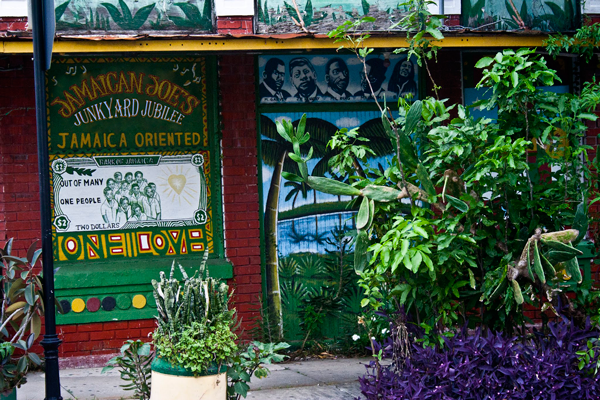
\includegraphics[width=0.5\linewidth]{images/SCP-100.png}
    \caption*{SCP-100的店面,外观}
\end{figure}

\bb{项目编号:}SCP-100

\bb{项目等级:}Euclid

\bb{特殊收容措施:}SCP-100的栅栏区域内有6名守卫进行巡逻,还有2名守卫负责监控内部和外部的仓库和住宅建筑,每3小时轮换一次。在SCP-100内发现任何未经授权的人员将被扣留和讯问,随后实行记忆消除并释放。

3名守卫,将留在SCP-100的店面内,每8小时轮换一次。店面正门应随时保持锁住,只有必要人员才持有钥匙。“私人财产”和“不得翻越”的警告标志应放置在店面前,以阻止任何司机停在SCP-100停留。

任何被SCP-100-1所制造的物品将被移出SCP-100并溶解成渣,除了SCP-100-2-A和SCP-100-2-B例外。若任何SCP-100-1变得不合作,SCP-100-2-A和SCP-100-2-B将被移出SCP-100直到SCP-100-1变得再次合作为止。

SCP-100内最大的两个仓库将被改装成基础研究设施。所有由SCP-100-1制造的物品,包括SCP-100-2-A和SCP-100-2-B,都可以用于研究目的。对SCP-100-1本身的测试则需要首席研究员的书面批准。

\bb{描述:}SCP-100是位于南卡罗莱纳州的一个废弃的废品堆放站,离█████████有80公里,最为知名的名字是“Jamaican Joe's Junkyard Jubilee”。该堆放站拥有5000平方米用栅栏围起的土地,包括两个仓库,一个店面,和一个小型的居住建筑,包括空地(neglected land,原意为被忽略的土地)和用于储存的面积。SCP-100收容有约1500辆汽车,包括已经被压扁和还没处理的,还有约1400公斤的零碎金属,价值约5000美元(3870欧元)。

SCP-100的异常效应体现在SCP-100-1和其造物上,包括SCP-100-2-A和SCP-100-2-B。项目会在SCP-100-1或其造物穿过SCP-100的栅栏时失去自主可动性,并保持该状态直到上述个体归还为止。

SCP-100-1是一个有自我意识的,有感知的,人形造物,由一系列钢管,未绝缘的铜线,和铝罐组成。SCP-100-1缺少进行书面或口头沟通的能力,尽管如此它有能力通过基本的信号(灯光)语言进行交流。SCP-100-1很大部分程度上不太关心外部销售和它被限制起来的信息。SCP-100-1似乎展示出制造技巧,并证明有能力操作诸如电焊机,钻头,和电锯,以及重型机械诸如车辆压缩机和铲车。

SCP-100-1展示出可以制造和其异常特性类似的个体,通过使用SCP-100内的各种材料,SCP-100-1创造了4个特殊动物-鬣蜥,鳄鱼,乌龟,和火烈鸟-尽管如此,SCP-100-1已知还创造过其他物种,诸如宠物。为了保持其顺从,SCP-100被允许持有2个物品,标记为SCP-100-2-A和SCP-100-20-B。

\begin{figure}[H]
    \centering
    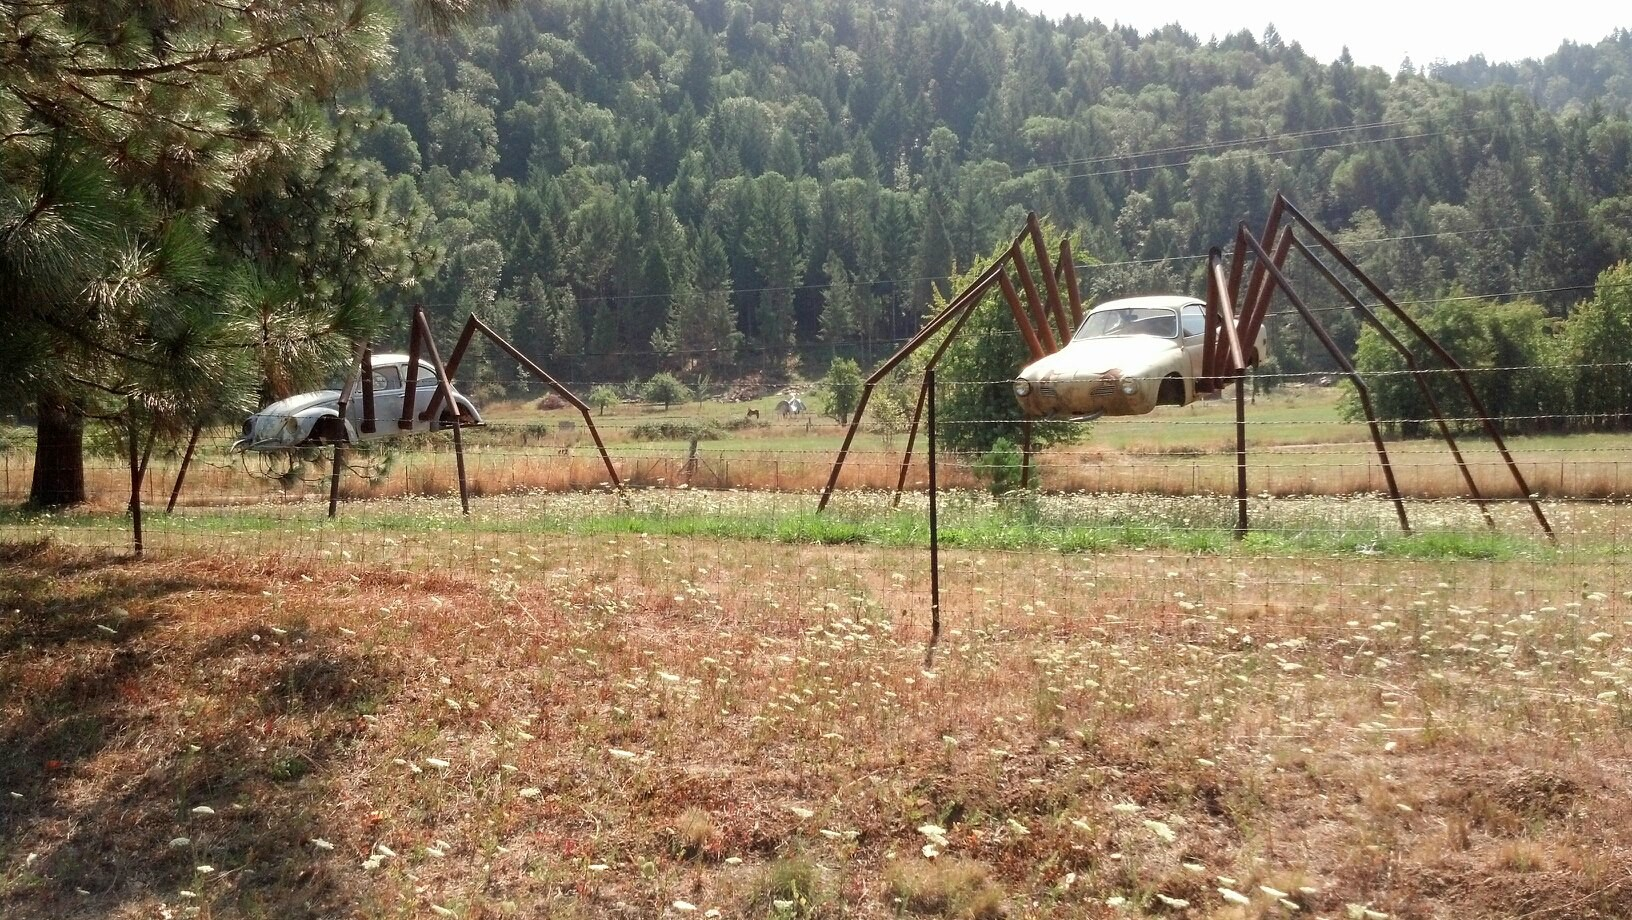
\includegraphics[width=0.5\linewidth]{images/SCP-100-2.jpg}
    \caption*{SCP-100-2-A和SCP-100-2-B正巡逻临时围栏的维修}
\end{figure}

SCP-100-2-A和SCP-100-2-B设计表面上类似于昆虫,假定是由SCP-100制造,因为它们在初次发现SCP-100时就占据了此处。SCP-100-2-A和SCP-100-2-B的背后分别印有名字“Raymone”和“Beatrice”。它们似乎同时作为同伴运作并守卫SCP-100,它们只在与SCP-100-1交流的间隔才停下,其他时间都在SCP-100的范围内巡逻。

SCP-100-1似乎服从一种仪式安排,每日重复以下行为。

\begin{itemize}
\item 在0800时到1500时,SCP-100-1进入SCP-100的店面,坐在柜台后面并试图和进入店面的人类谈价。偶尔的,SCP-100-1会较早的回到堆放场内,理由未知。
\item 在1500时到1600时,SCP-100-1通过模糊手势和脚步运动进行和SCP-100-2-A和SCP-100-2-B进行交流。交流内容包括装饰,修理,以及类似“取物”和“捉迷藏”的行为。
\item 在1600时到2000时,SCP-100-1进行各种工作,包括从SCP-100内取得材料,清扫和维护工具以及重型机械,并清扫SCP-100内建筑物的内部和外部。
\item 在2000时到0000时,SCP-100-1进行假定为休闲的行为,行为包括制造新物品,和SCP-100-2-A和SCP-100-2-B交流,在SCP-100内巡逻等。
\item 在0000时到0080时,SCP-100-1进入住宅建筑,并在此期间一直坐在书桌后面。
\end{itemize}

若在SCP-100-1坐在柜台后时有人类进入SCP-100的店面,SCP-100-1将试图与他们交易,使用各种手势来表达意思。SCP-100-1大部分情况试图出售废品,它自己的造物,或修理服务,尽管如此它知道如何购买废品。尽管SCP-100-1无法阅读,但是它在销售中显示出有基础的数学计算能力。

SCP-100-1所做的销售显示出某种程度的不公平。SCP-100-1会故意出售用便宜金属制作的有缺陷的天平和有污渍的废品堆,并似乎有关于SCP-100效应的知识,因为SCP-100-1不停重复出卖造物,尽管其自主移动性在离开SCP-100后就消失了。遭遇SCP-100-1将会面对窘迫和冷漠,其墙上贴着标语“不退货,伙计!”,无论SCP-100-1的情绪反应如何。

SCP-100发现于11\slash 09\slash 76,当时有报告有奇怪的机械在废品堆放场内活动。这些流言被视为都市传说,而基金会派了一名特工去SCP-100去冒充土地所有者,直到收容通过不动产购买完成。一道木质栅栏沿着之前SCP-100的栅栏建立起来,在店面里装上了单面窗户(从外面无法看见里面),而一条穿越附近█████████镇的高速公路使得大部分公众交通改道。

\bb{附录100-A:}记录显示此处拥有者为“Joseph Duval”,其邮政地址也使用同样的名字。当地账务公司报告其账单在SCP-100发现的3个月前停止了,只留下SCP-100-1,SCP-100-2-A,SCP-100-2-B,以及数只假定被SCP-100-1创造的鸟类和犬类个体。对建筑物的初次扫除发现住宅建筑的大部分都空空如也,唯一显示前主任的信息是一张写在纸条上挂在店面门上的纸条。(见\bb{文件100-A})

\bb{事故100-A:}在06\slash 03\slash 05,SCP-100-1创造了一个有自我意识,10厘米高的人形,这是SCP-100-1第一次创造人形。其在该造物上用了比其他造物更多的努力,该造物上拥有极其精细的细节,包括面部特征,和印在造物背后的“J.J.”字样,造物的大部分都是由不锈钢制成。SCP-100-1在时间表间隔期间将造物放置在店面的柜台上,并互相使用各种手势进行明显的交流。在和造物进行交流之后,SCP-100-1在SCP-100内的住宅建筑内坐了将近10天。

\bb{文件100-A:}下列是在SCP-100内回收的备忘的一份拷贝。

\begin{scpbox}
\centering
出去吃午饭,请找助手-J.J.
\end{scpbox}



\include{editors}

\includeonly{
cover, 
part00/index,
part01/index,
part02/index,
tale/index,
authors/index,
compilation/index,
appendices/index,
changelog,
}

\hypersetup{
pdftitle={SCP基金会内部人员手册},
pdfauthor={SCP基金会中国分部}
}

\begin{document}

% 对话框初始设置
\tcbsetforeverylayer{
arc=0pt, outer arc=0pt, 
left=10pt, right=10pt, top=10pt, bottom=10pt, 
after skip=12pt, 
parbox=false, breakable,
}

% 这两个宏用于文档未翻译的模板,会在各 chapter 中重新定义使用
\newcommand{\DOCNAME}{}
\newcommand{\DOCSLUG}{}

\frontmatter

\include{cover}

\tableofcontents

\mainmatter

\setcounter{part}{-1}

\part[SCP-001提案]{
	SCP-001提案
	\protect\footnote{编者\QIS :\\ 
	SCP-001有多份提案,遂单独成一部分。\\ 
	又由于第一篇SCP-001其实是目录,所以内部文章编号从0开始。\\ 
	另外,由于大部分SCP-001提案旨在说明基金会的起源,推荐刚接触SCP系列的新人先跳过。在看过几十个SCP档案,对基金会设定有初步了解后再回来看001,可以获得更好的阅读体验。}
}

\setcounter{chapter}{-1}

\chapter[{SCP-001 等待解密[已锁]}]{
	SCP-001 Awaiting De-classification [Blocked] \\
	SCP-001 等待解密[已锁]
}

\label{chap:SCP-001.0}

\cl{

\GG{在管理者的命令下}

\GG{此文档已被列为}

\bb{\Hg{\wred{最高机密}}}

}

\hr

\begin{scpboxbr}
\bb{通用说明 001-Alpha}:为防止SCP-001的真相泄漏,多份/零份伪造的掩盖文件与该份/多份真正的001文件一并储存。所有涉及到SCP-001本质的文件,包括一份/多份假文件,均由模因抹杀药物保护,如有未授权人员查看,将立刻导致心脏骤停死亡。除非是受到████-███-██████的指令,否则将SCP-001的内容透漏给公众者将会被处决。
\end{scpboxbr}

\hr

\cl{

\bb{\Hg{\wred{警告}}}

任何未经授权之人员访问该文档将立即被\bb{BERRYMAN-LANGFORD}模因抹杀触媒处决。在未接种合适模因疫苗的情况下向下滚动页面将立刻导致心脏骤停死亡。

\bb{\GG{\wred{你已经被警告过了。}}}

}

\hr

\newpage

\begin{figure}[H]
	\centering
	
\includegraphics[width=\textwidth]{images/SCP-001-0.jpg}
\end{figure}

\cl{

\bb{模因抹杀触媒启动}

\bb{检测到生命迹象}

\bb{解开安全锁}

\ii{欢迎,已获授权的人员,请选择您要看的文件。}

}

\hr

\definecolor{fcfdfb}{HTML}{FCFDFB}
\begin{scpboxbrc}[colback=fcfdfb]

\hyperref[chap:SCP-001.sheaf.of.papers]{代号:Jonathan Ball} - 资料卷

\hyperref[chap:SCP-001.the.prototype]{代号:Dr. Gears} - 原型

\hyperref[chap:SCP-001.the.gate.guardian]{代号:Dr. Clef} - 守门者

\hyperref[chap:SCP-001.the.lock]{代号:qntm} - 锁

\hyperref[chap:SCP-001.the.factory]{代号:Bright} - 工厂

\hyperref[chap:SCP-001.the.spiral.path]{代号:Dr. Mann} - 螺旋路

\hyperref[chap:SCP-001.the.legacy]{代号:Dr. Mackenzie} - 遗物

\hyperref[chap:SCP-001.the.database]{代号:S. Andrew Swann} - 数据库

\hyperref[chap:SCP-001.the.foundation]{代号: Scantron} - 基金会

\hyperref[chap:SCP-001.thirty.six]{代号:Djoric/Dmatix} - 三十六

\hyperref[chap:SCP-001.keter.duty]{代号:Roget} - Keter任务

\hyperref[chap:SCP-001.ouroboros]{代号:djkaktus/TwistedGears} - 衔尾蛇

\hyperref[chap:SCP-001.a.record]{代号:Kate McTiriss} - 一份记录

\hyperref[chap:SCP-001.past.and.future]{代号:Kalinin} - 过去与未来

\hyperref[chap:SCP-001.the.consensus]{代号:Wrong} - 一致意见

\hyperref[chap:SCP-001.when.day.breaks]{代号:S. D. Locke} - 破晓之时

\hyperref[chap:SCP-001.gods.blind.spot]{代号:Spike Brennan} - 上帝的盲点

\hyperref[chap:SCP-001.normalcy]{代号:WJS} - 常态

\hyperref[chap:SCP-001.the.world.at.large]{代号:BILLITH} - 世界,收容失败

\hyperref[chap:SCP-001.dead.men]{代号:Tanhony} - 死人

\hyperref[chap:SCP-001.the.worlds.gone.beautiful]{代号:Lily} - 美丽新世界

\hyperref[chap:SCP-001.the.scarlet.king]{代号:Tufto} - 深红之王

\hyperref[chap:SCP-001.a.simple.toymaker]{代号:Jim North} - 普通的玩具师

\hyperref[chap:SCP-001.story.of.your.life]{代号:I.H. Pickman} - 你一生的故事

\hyperref[chap:SCP-001.a.good.boy]{代号:The Great Hippo (feat. Peppersghost)} - 好孩子

\hyperref[chap:SCP-001.project.palisade]{代号:weizhong|thedeadlymoose|Drewbear|Dexanote} - 围栏计划

\hyperref[chap:SCP-001.O5.13]{代号:Captain Kirby} - O5-13

\hyperref[chap:SCP-001.fish.hook]{代号:Pedantique} - 鱼钩

\end{scpboxbrc}


\input{part00/001.sheaf.of.papers}

\input{part00/001.the.prototype}

\chapter[SCP-001 守门者]{
	SCP-001 Dr. Clef - The Gate Guardian \\
	SCP-001 守门者
}

\label{chap:SCP-001.the.gate.guardian}

\begin{figure}[H]
    \centering
    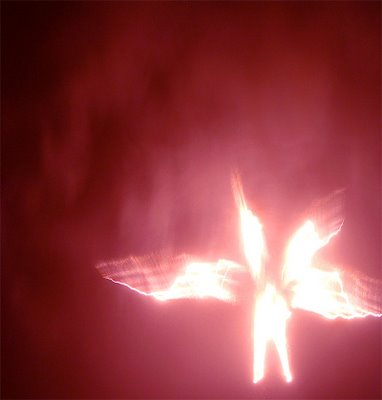
\includegraphics[width=0.5\linewidth]{images/SCP-001-the-gate-guardian.jpg}
    \caption*{在Site-0的有利位置拍摄的SCP-001图片。注意位于图片上方到两侧的四个燃烧的“翼”状附属物。}
\end{figure}

\bb{项目编号:}SCP-001

\bb{项目等级:}Euclid\slash Keter

\bb{特殊收容措施:}由于SCP-001的特性,没有任何监禁措施是必要的。对SCP-001的不间断监控必须在预定地点(Site 0)以外的安全距离(10公里以上)持续进行。Site 0的位置只有当前的SCP总管理员和一位被指派从Site 0监视SCP-001的信仰亚伯拉罕系信仰的监察者级探员(O5-14)所知晓。这位探员被授权当SCP-001开始活动时采取任何必要手段,并且需要当SCP-001的行为出现任何变化时立即警告总管理员和其他监察者级探员,因为这可能导致PATMOS XK级世界末日情境的开始。

如果SCP-001以任何形式开始活动,工作人员被要求立即考虑Patmos序列紧急指令。紧急指令Patmos的解法算式被保存在Site 0的被指派的监察者处,并且只在SCP-001开始活动的情况下才传输到SCP基金会的办公室。在紧急指令Patmos当中有着一项或多项重要角色的工作人员被建议做好以下准备工作:

\begin{itemize}
\item 和一种或多种有组织的亚伯拉罕体系的宗教保持良好关系。
\item 随身携带或手持以下物品:圣水,一件由一位主教以上等级的亚伯拉罕体系宗教教士所祝福过的玫瑰念珠,十架苦像,十字架,或其他象征物,一份亚伯拉罕体系宗教经本(托拉,圣经,古兰经),以及可随身携带的标准应急补给品(避难包)。
\item 在千禧年降临情境下,所有重要的人员都被指派一名非亚伯拉罕体系宗教信仰的副手,这名副手将会被告知原人员的紧急指令Patmos的备份的地址以及模因抹杀媒介的接种,并且准备好在必要情况下接替原职的任务。
\item 对所有其它涉及到可能的PATMOS XK等级世界末日情境的SCP保持熟知。
\end{itemize}

\bb{描述:}SCP-001是一个人形的个体,大约身高七百(700)腕尺,位于底格里斯河和幼发拉底河交口处附近的一个秘密地点,关于这个个体有下列已知特征:

\begin{itemize}
\item 从个体肩膀、背部、脚踝和腰部伸展出的数个发光的翼状形态附属物。尽管不能进行精确的计算,大部分的观察者给出的翅膀数目从二(2)到一百零八(108)个不等,平均数为4。
\item 一件武器,可能是一把剑或者刀(SCP-001-2)。通过光谱分析,这把武器从外观上看放射着温度足以匹敌太阳的火焰,尽管这极度的高温看起来并没有给周围的地区造成任何毁坏。任何接近SCP-001一公里以内的个体会立刻被这件武器攻击并彻底消灭掉。对SCP-001采取的任何形式的敌意行为都会导致攻击者的毁灭,不管距离多远。(参见事故报告:印度洋潜艇导弹实验,2004年12月26日)
\item SCP-001呈站姿,双手于身前握持SCP-001-2让其剑尖向下,低头呈祈祷状。自从建立者在{[}数据已编辑]年前所记载至今,SCP-001未曾改变过这一姿势。
\item 暴露在SCP-001面前的人类报告说在脑内听到了一个声音,向他们下达无法违抗的指令。最常见的指令是“忘记”,导致实验对象从SCP-001附近走开并且没有留下任何遇到过它的记忆。但是,在罕见的情况下,也会出现其它指令:最著名的指令就是下达给建立者的(“准备”)促使他成立{[}数据已编辑]来分类和保管所有对当前人类存在造成严重威胁的超自然以及异常物品。这就是现在被称为SCP基金会的组织。
\item 观察者报告说SCP-001是站在一扇巨大的门前面。长距离摄像偶然间探测到门内是一片田园树丛,里面还有无数的其他和SCP-001构成相类似的个体,还有几棵构成未知的果树。值得特别注意的是在树丛中间的地方有两棵巨大的果树:其中一棵,被注意到看上去是一棵普通的苹果树,但是另一棵树上的果实则完全不为地球上所知,被描述为{[}数据删除]。
\end{itemize}

建立者公开承认他相信SCP-001所守卫的门可能就是{[}删除],根据和古巴比伦文书和死海古卷的对比可知。在这个前提之下,我们可以推断被命名为SCP-001的个体可能就是{[}删除]

\hr

\uu{\bb{附录001-a:} 重新实验: SCP-001-2的有效杀伤范围}

\ii{1.实验A:一名D级人员被要求尽可能徒步接近SCP-001。}\\
结果:在和SCP-001发生视觉接触时,实验体被命令“离开”。实验体立刻转身离开SCP-001.尽管重复多次指示要求继续实验,D级员工拒绝遵守命令并被处决。在D级员工被处决时,所有涉及到实验的研究人员都被未知的力量消灭,推测是SCP-001-2。

\ii{2.实验B:一台遥控研究用机器人被控制从地面接近SCP-001。}\\
结果:在距离SCP-001一公里的时候,研究机器人被消灭了,推测是SCP-001-2的所为。所有后续的遥控侦查尝试都得到了同样的结果。

\ii{3.实验C:100个预先编程的研究用探针被命令从多个角度同时接近SCP-001}\\
结果:协调非常成功,100架探针同时通过了一公里标志线。然而,100架探针同时被SCP-001-2所消灭了。指派在Site 0的观察者报告说SCP-001-2看起来“同时向所有的方向发动了攻击”。SCP-001在此过程中姿势没有发生任何变化。

\ii{4.实验D:从3千米远处发射的线导导弹}\\
结果:SCP-001-2在武器穿过一千米距离时将其消灭,与此同时也消灭了发射场并杀死了所有人员。

\ii{5.实验E:从SCP核潜艇“鹦鹉螺号”上发射的多弹头洲际弹道导弹}\\
结果:参照印度洋潜艇导弹实验报告,2004年12月26日

\ii{6.实验F:\hyperref[chap:SCP-076]{SCP-076}和Omega 7特遣队被指示徒步接近SCP-001。}\\
结果:\hyperref[chap:SCP-076]{SCP-076}拒绝执行任务,尽管并没有得知任务的性质。在被问到为什么的时候,SCP-076回答说“不干,就是不干。”

\ii{7. 实验G:\hyperref[chap:SCP-073]{SCP-073}。由于实验F的结果,SCP-073在到达Site 0之前没有被告知他的目的地}\\
结果:SCP-073徒步接近地点。在看到SCP-001的时候,SCP-073变得非常悲伤并要求中断实验。SCP-073被命令继续实验。这时,SCP-073额头上的符号变成了{[}数据删除]。实验由于{[}数据删除]的缘故被终止。参见附录001-aa

\ii{附录001-aa:通过总管理员的命令,不再对SCP-001进行进一步的实验。不许再让任何SCP暴露在SCP-001前。SCP-001不可用于处理危险的SCP。细节部分请阅读修订版收容措施。}

\hr

\hr

\bb{附录:}在 ██-██-████,基金会工作人员接收到下面这条错误信息。

\begin{scpbox}

启动紧急指令 PATMOS-OMEGA

请注意:所有基金会工作人员

今天早上大约 ████:██:██ 的时候收到Site 0传来的下列信息。

\mono{SCP-001离开了它的位置。大门开启了。它们在前进。}\\
\mono{哦上帝啊,这真美……}

\mono{主的国来了主的国要来了主的国已经来了主将统治直到永永远远主的国来了}\\
\mono{主的国要来了主的国已经来了主将统治直到永永远远主的国来了主的国要来}\\
\mono{了主的国已经来了主将统治直到永永远远主他是上帝主他是上帝主他是上}\\
\mono{帝主他是上帝主他是上帝主他是上帝主他是上帝主他是上帝主他是上帝主}\\
\mono{他是上帝主他是上帝主他是上帝\bb{听吧以色列主我们的上帝主是唯一的}}

由于这一事件和最近\hyperref[chap:SCP-995]{SCP-995}的破裂,\hyperref[chap:SCP-616]{SCP-616}的开启和\hyperref[chap:SCP-098]{SCP-098}的启动的共同作用,基金会被要求立即开始准备应对XK级世界末日情境。\hyperref[chap:SCP-076]{SCP-076}和\hyperref[chap:SCP-073]{SCP-073}要立即被关押。所有人员解锁和编译紧急指令Patmos-Omega,并且遵从里面的命令。Site 19要被确保,并且一切非必要的SCP和人员都要被立即处决或销毁。重复,由于这一事件和最近\hyperref[chap:SCP-995]{SCP-995}的破裂,\hyperref[chap:SCP-616]{SCP-616}的开启和\hyperref[chap:SCP-098]{SCP-098}的启动的共同作用,基金会被要求立即开始准备应对XK级世界末日情境。\hyperref[chap:SCP-076]{SCP-076}和\hyperref[chap:SCP-073]{SCP-073}要立即被关押。所有人员解锁和编译紧急指令Patmos-Omega,并且遵从里面的命令。Site 19要被确保,并且一切非必要的SCP和人员都要被立即处决或销毁。重复,由于这一事件和最近\hyperref[chap:SCP-995]{SCP-995}的破裂,\hyperref[chap:SCP-616]{SCP-616}的开启和\hyperref[chap:SCP-098]{SCP-098}的起动的共同作用,基金会被邀球立即开始准被硬队XK级世界末日青境。\hyperref[chap:SCP-076]{SCP-076}和\hyperref[chap:SCP-073]{SCP-073}要立即被关押该隐和亚伯我的两个儿子,我来了所有人员解锁和编译看呐,我站在门前敲那门并且如果任何任任何ansdfysffollow aall alla khaf3242!\$\$@并且是是一个新的天堂一个新的地球和果实的\\
\textasciicircum \&@\#\$@\#@\#\$@\#\$███████\\
█████████\\
█████████\\
█████████\\
███{[}信号丢失]

\end{scpbox}

通过联系Site 0,O5-14回复说没有这样的消息从他那里发出并且SCP-001也依然静止。这条传输起初被认定为是恶作剧。然而,进一步的检验显示这条传输的时间标记在{[}数据已更改]年后的未来。因此可以推论{[}数据删除].

\hr


\input{part00/001.the.lock}

\chapter[SCP-001 工厂]{
	SCP-001 Dr. Bright - The Factory \\ 
	SCP-001 工厂
}

\label{chap:SCP-001.the.factory}

\bb{SCP-001是一名O5的故事}

晚上好,博士。

不,不,不用站起来。对,没错,我就是那个人。既然你我都明白,我们还是不要在这件事上耽搁太久了。你只知道我的号码,而我对你的了解能让我造一个你的复制品,连你妈都分不出来谁是真的。不对,这不是一个威胁,只是一个事实。

现在,关于我为甚么来到这里,你似乎碰巧发现了一些在你的权限之上的东西。恩,不对,碰巧发现不是一个正确的词。发掘?或许更准确。而你正在接近一个危险的临界点,到那时任何进一步的发掘都会以一个致命的枪伤作为句号。这对于我们的事业将会是个可悲的情形,因为除此之外,你依然是一个非常棒的研究员。因此,你将会得到只有极少数基金会中人曾得到过的东西:一个解释。

没错,当你第一次探索SCP-001时,我们就已经警惕了。每一个曾短暂接近它的研究员都会忍不住往里面看看。大多数都满足于他们发现了带著火焰剑的天使,它已经埋在足够深的等级下了。但接著你开始调查The Factory,我们就知道你不会停下。所以,我将告诉你那个清晰而简单的答案。

The Factory就是SCP-001。

但这个真相是永远不会被写下来的。这是我早在基金会创立初期就决定的,而且我仍然坚持这个决定。你们这些研究员实在太有好奇心了。我不知道哪件事更令我恐惧:我们永远不会了解The Factory,还是我们有一天会了解它。好吧,我知道你渴望知道更多。

The Factory是在1835年建立的。那时它叫做The Anderson Factory,因一位非常富有企业家,其创始人詹姆士・安德森(James Anderson)而得名。它是,呃,我只能告诉你它是在美国成立的,并且是到那时为止最大的工厂,最宽处有一英里(1.6公里),所有建筑都有3层楼,大门前还有一个专供Anderson使用的7层高塔。它被设计为工厂的最终形态,能够处理所有的东西,包括员工的住房。人们可以在这里出生、工作、生活、死亡而不需要离开工厂的范围。人们的工作范围极广:从牛的养殖到屠宰,纺织,以及世界上一切工作。

但是,没人知道James Anderson是一个撒旦的崇拜者。他有很大可能信奉一些异教的神灵。他对于工厂里建筑的位置和机器的摆放有非常严格的要求。工厂的幸存者声称建筑的地板上刻满了只有当鲜血流过时才能看到的神秘符号⋯⋯当然,幸存者还告诉了我们一些其他的东西。他的钱是从工人阶级的血汗,甚至工人阶级的尸体上赚来的。他在日记里认为工人不过是一种比人类低贱的东西,放在地球上就是来为他服务的。

当然了,在那个时候还没有人了解他的邪恶嗜好,因而他的工厂吸引人们蜂拥而至。有一个地方能同时解决工作和生活?好吧,人们理所应当的想要进去!至于严苛的工作时间、恶劣的工作环境,残酷成性的保安,和其他所有的一切古怪,都没有关系。工厂的工人们被迫一天工作16个小时,从日出干到日落,星期天才能停工。工人甚至没有独立的房间,要与另外8人分享房间,三班倒的轮流去睡觉,保证工厂全天有人干活。从没有人听说过医疗。如果你因为你的职责受伤了,你只会被要求继续干下去,那些伤得太重而无法工作的人会被保安拉走,没人再听说过他们。

整整40年,安德森工厂大量制造了所有人类所需的产品。肉、衣服、武器。不会有人介意牛肉里面可能混合著人肉。别去想武器是在鲜血里淬火的。不用去管衣服的颜色是来自⋯⋯呃,你懂的。确实有泄漏出去的谣言,但是那些产品那么好,干嘛抱怨呢?直到有人逃了出来。

我从没有见过那位勇敢追求自由的灵魂,不过她想尽办法见到了格兰特总统。在1875,格兰特总统寻求我的帮助。当时我是⋯好吧,这不重要。我只会告诉你我是一名军人,某种军人,而且我的伙伴们也是。我们有150位好兄弟和几位姐妹,接一些常识不会接受的工作。我们清洗过一些南部联盟的顽固份子,以及我们在南方找到的更坏的东西。于是,我们做了一些调查,并不喜欢我们看到的东西。我们闯进了工厂,承担这项重担。

我并不完全记得那个工厂陷落的夜晚了。许多记忆在我的脑子里搅成一锅粥。一些片段常会闪现出来,有时是许多人被一根锁链拴在一起,活在死亡的边缘,你极难分出来哪块肉是谁的。孩子们活在机器的支配下,身上大部份的肉都已经被转轮、齿轮之类的机器从骨头上剔掉了。

没事,我没事。我已经很久没有回忆这些东西了。工厂的保安并不是问题,但Anderson的作品很快出现在我们面前。他把很多受伤的工人拉走,然后,嗯,在他们身上做试验。人类,如果你还能把他们称为人的话。许多种类的手臂缝在他们身上,有些还装上了动物的身体,是超出人类最荒诞邪恶的噩梦的恐怖怪物。他们不断涌来,不能称之为活著的生物一波波的出现。那个晚上我失去了许多战友。后来我们发现了Anderson的培育地下室,一个只有8岁的小女孩被绑在墙上,被变成了-

对不起。即使在超过一百年后的今天,这些记忆仍仿佛满是血色。我们找到了蜷缩在他的办公室里的Anderson,用他的肠子把他吊死在高塔的窗外。在他死亡的过程中,他不断狂笑,大叫说这不是问题,我们可以杀了他,但他的工厂,The Factory,不会停工。24小时后他仍狂笑不止,我们最终放他下来,掏出他的内脏,每件都切成四块,再把剩下的部分烧成灰烬。整个过程他一直在狂喷亵渎之词,我不想回忆那些话。

我们用了一个星期去清理这片区域、释放工人、纪录每一件我们在地下室和昏暗的房间中找到的东西。我们拿出那些看上去有用的东西,存放在大门旁的一座房子里。尝试去弄懂每一件东西。我们有150位伙伴在那个晚上进到地狱里,只有93人出来。而一星期后只剩下71人了。

而那些我们在里头找到的东西,我的天哪。好吧,你已经在基金会工作过一段时间了,他们应该不会让你太过惊讶。不过当时我们可是第一次看见会发射真子弹的玩具枪;能把碰到它的皮肤剥下来的摇摇;只对人体起作用的大锤;一种跑得比当时所有东西都快的骨骇马;如同暗夜亲自编织的斗篷,能让穿上它的人来到一个虚无的维度,那里有⋯⋯我又失态了。我们找到了很多器具,既不可思议,也很可怖。接著我们面临著一个抉择。

我把队伍里最高级的几个人召集来,恩,我想想,我们最好称他们为长官。我们设法去弄清楚我们接下来该干甚么。每个人都有不同的想法。Chaplain变得有点疯疯癫癫的,觉得这些对象都是神赐予我们的奇迹,要像对待圣物一样崇拜它们。Marshall还有他的跟屁虫Dawkin认为这些是工厂造出的好宝贝,要继续制造它们然后卖给出价最高的人。Injun,我们都叫他Bass,因为他的声音像男低音一样,说这是令人厌恶的东西,声称无论如何他都会搜寻并销毁所有他找到的东西。Smith想到我们应该先释放所有劳工然后把他们带回总统那里。我们在那里争吵了几小时,几天,想办法解决这些。至于我,我觉得我们正坐在一座金矿上面,行了别那样看著我。虽然很危险,但我们可以利用这些东西,这些对象,去搜捕那些我们曾在南方偶然遇到的骇人之物,以及其他需要全世界共同应对的怪物。让这个工厂用在正道上,一个可以收容这些东西的地方,想办法让它们为人类同胞服务,至少保护人类免受其害。

我想你应该已经猜到接下来发生甚么了。Chaplain在一天晚上带著他的崇拜者偷偷离开了,还拿走了几件小物品。我们把Marshall撵走因为我们发现他在⋯⋯滥用职权。他保证他一定会报复我们。卑贱的Dawkin该死的带领他们那群人和一些重要物品离开了。Bass和他的人努力的去点燃工厂想把这些该死的东西烧掉却徒劳无功,后来他们也走了。Smith也跑去向总统汇报。我最终让他保证会告诉格兰特工厂已经彻底毁掉了。我有一个大计划。

当然了,想要实现一个大计划是有点困难,特别是只有12个人和你一起工作的时候。不过我们还是开始了。

计划运行得很顺利,暂时的。我们已经有了这些神奇的玩具,想要招人跟我们一起工作就变得很容易了。在那个时候,离开电就像走出村子一样简单。我们知道我们需要甚么,也知道我们会变成甚么。

Leventhal开始得到我们的支持。他搞了个小发明,弄到了一大笔投资,都很有用。White和Jones则开始得到我们⋯⋯其他人的支持。在我们搞定工厂之前的工作中我们已经发现了一些与某些人有关的有趣的东西。那些当权者不会想要泄漏出去的秘密。而且,因为我们新的根据地让我们能更好的守住这些秘密,越来越多的人跑来想让我们处理他们的秘密。勒索是个肮脏的词,不过很管用。Bright,Argent和Lumineux著手纪录项目。Light和Bright的老婆,她们是护士,确保我们保持健康。嘿。算了,只要记住Light就可以了。在那个时代,她在卫生方面有著许多独特的见解。Czov,Fleischer和Carnoff处理军队训练的事。Tesla和Tamlin负责找出利用项目的方法,在不会暴露我们的情况下。

我们的效率高得惊人。一个城市围绕著The Factory建立起来了,我们开始叫它作Alpha站点,而且它还是自给自足的。特工、研究员、各种熟练技工⋯⋯当然,我们不依靠那些当权者,而是靠这些工作人员。我们不断发展壮大。

…

不好意思,我已经是一个老头了。我知道我不愿意正视它,不过我的身体在撒谎。我的脑袋⋯⋯并不总是记得准确。有时我会沈浸在回忆里。事情变得令人困惑。不过在很长一段时间里,一个显而易见的事实是:我们在利用the Factory。总是能在里面找到更多的空房间去储存东西。那个时候我们还用“东西”来称呼它们。不需要跳过这段,不需要。我们认为我们已经驯服了the Factory。这是我不停止这项工作的原因之一。但如果现在有甚么事情是我确信的,那仍然是人类永远不能驯服这些东西。收容它们就好了,就像那位你我都曾见过的Able一样,驯服它们?不可能。

大约十年之后,我们已经组织的很好了。13位创始人只用编号作为代称,不再用名字。大家都知道怎么样让事情运转良好。并且,如果有一两件东西在the Factory里消失了,依然如此?而且有时是D级人员消失?甚么?没错,我们那时就已经有D级人员。用过就丢(Disposables)。这就是字母D的由来。肯定要有一些人给我们试验那些东西,Tesla和Tamlin对此非常坚决。但是,没错,有时我们会失去一些无关紧要的人。Adam⋯⋯抱歉,是Dr. Bright喜欢说这是the Factory在让我们“留下买路财”。你不可能甚么都不付出就有收获。

到了1911,一切都失败了。那些家伙⋯⋯我们称之为小仙子。那些家伙全族都栖息在我们旁边。它们看上去跟你我长得一模一样。唯一明显的区别在于对铁过敏。对,这就是为甚么我们叫它们作小仙子。不过,你从没听说过它们是很正常的。为甚么?因为那个时候基金会就已经把它们全族都灭绝了。连根带叶的。并且我也动手了。

我们已经被它们当成猎物一段时间了。我们之前也碰到过它们几次,都把它们成功搞定了。所以,当某位王室成员来向我们寻求帮助时,我们当然会想要让他们欠我们人情。人人都喜欢让别人欠自己人情的。我们派了一对人员去帮忙,稍微关注了一下,觉得这不过是一次狩猎派对。下次我们看见队员们和那个王室成员,他们的头都被插在杆子顶,系在小仙子骑的生物的马鞍上,它们来攻击the Factory了。

很可怕。

三个字,信息量太大了。我从来没有⋯⋯抱歉,请给我一点时间。我从来没有告诉任何人这个部分。你应该觉得你很幸运。而且,如果你把我将要告知你的事情的任何一点点说给其他人,我不仅仅会杀了你,还会干掉那些跟你分享DNA的人,用我能想到的最可怕的方式。跟我那时会在你身上干的事情比起来,你会觉得110蒙托克程序不过是在花园里散散步而已。

我们输了。那些家伙冲了进来,毁灭了我们。骑在我们的炮台上,屠杀我们的人员,无视我们的武器就像它们不存在一样。我眼睁睁看著我左右的13位伙伴倒下,只是努力的想要保护the Factory。那我呢?我,他们的领导者,他们的朋友,他们的父亲般的长者?Bright四个孩子的教父,知己,有时是情人,平常是聆听他们忏悔的神父?我跑了,跑得就像一个惊恐的小男生,深入the Factory那黑暗的五脏六腑中。我被那些家伙追著,只有一步之遥。我甚至能听到他们跟在我后面,感觉到他们脖子上的气息,然后⋯⋯

我来到一扇我从没有看过的门前。黄铜大门,覆盖著一些类似阿拉伯字母的符号。我向来对语言一窍不通,特别是那些狗屎穆斯林用的鬼画符。不过我当时也管不了那么多了。它们正向我冲来,我立刻拉开门钻了进去。里面的一切⋯⋯都不一样。那是一种平静安宁的感觉,似乎没有东西能在那里伤害我。光线是像这样的暗红色,不过仍然觉得正常。我耳朵里充满了稳定而持续的巨大心跳声。在我的面前,是Anderson的遗骸。接著它开口向我说话,不过我打死也不会说出确切的话。更重要的是它说的话的价值,而不是细枝末节。它给了我一个希望。他告诉我⋯⋯他告诉我说每一件我们使用的the Factory出品,不论我们是用它们来做甚么,都在喂养它。帮助它成长。但是,如果那群小仙子攻陷了the Factory,它们会毁掉它,我们都不能让这件事发生。它提出一个⋯⋯方案。它能清除这件事。让它从没有发生过。我们只需要献出⋯⋯我们自己。

我并不想接受。我知道这绝对不安好心。但接著,我眼前浮现他们,我的家人,我的朋友,都死了。死在那些混蛋的手上⋯⋯我同意了。它笑了。然后我发觉自己又回到了城墙上,看著一大群小仙子爬过山峰。我的基金会满血复活了。我手上拿著一把武器。我就不用细节吊你的胃口了,总之我们轻松战胜了它们。接著,手里拿著那些新武器,继续屠杀它们,每处它们栖息的地方,每处它们繁殖的地方。我的O5的同志们提出了疑虑,觉得我们应该留下来一点,以免以后我们可能会用到它们⋯⋯我否决了。

我们离开了the Factory。紧闭大门。把我们的东西移出来。我们把它们的名字从东西变成了特别收容协定(Special Containment Protocols),专注于收容它们,而不是⋯⋯干点别的甚么。其他人都很好奇,不过都了解我一定有我自己的理由。我用木板把the Factory围住。关上锁好。把它埋在成吨的碎石瓦砾下,声称它实在是太危险了。我觉得⋯⋯觉得我已经侥幸逃离它了。直到我在我桌上发现了一件东西。众多能发射真子弹的玩具枪的其中一把。而且上面有著the Factory的标志。

⋯⋯我偶尔派人进去过,去查看里面可能在做些甚么。最近一次派人时,那里是空的。但我们依然继续在外面发现Factory的物品。我忍不住想到底还有多少我们没有发现。和那些使用它们,并把它们藏起来的人。我回想起那具尸体说过每一次使用物品都会给the Factory提供能量。我从没有问过他它“是给甚么的能量?”我不认为我会想要知道。

我们献给送给了它甚么?D级人员,大部份的。你以为那些尸体去哪了?总得有个地方。尸体被我拿走,然后就消失了。所有人都觉得我是个天才,能想到解决这问题的办法。有时⋯⋯有时我还不得不喂给他一些其他东西。研究员。特工。他们从不知道它正在靠近。它只是伸出手来然后把他们拉进去。

不过,我们终究是在这里做著正确事情。不论the Factory想干甚么,不论它是甚么⋯⋯我们做得对。我不得不相信这一点。

现在你知道了。你高兴吗?我看不像。为甚么要告诉你?我正在老去,Everett。如果我死了,总要有人去继续喂它。或许你会不一样。或许你能找到反抗它的办法。

⋯⋯但我很怀疑。


\chapter[SCP-001 螺旋路]{
	SCP-001 Dr. Mann - The Spiral Path \\
	SCP-001 螺旋路
}

\label{chap:SCP-001.the.spiral.path}

\begin{figure}[H]
	\centering
	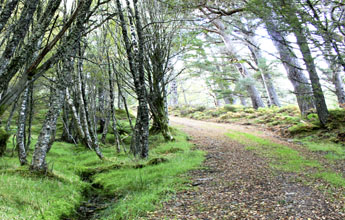
\includegraphics[width=0.5\linewidth]{images/SCP-001-the-spiral-path.jpg}
	\caption*{SCP-001的一部分}
\end{figure}

\bb{项目编号:}SCP-001

\bb{项目等级:}Embla

\bb{特殊收容程序:}SCP-001于[已编辑]州,Site 0就地收容。一道围篱沿著SCP-001的可观察半径筑起。为了安全起见,Site 0随时都需布署五名或以上的武装守卫以防止未经授权的进入。邻近的物理实验室也需随时运作以研究任何异常。

一块刻有提醒标语的金属告示牌应随时维护以保持在最佳状态。任何损伤都需立即回报以进行修补。

\bb{描述:}SCP-001是一条位于林中的环状砾石小径。以逆时针方向行走时,路途会是持续的上坡,就算通过起始点亦然;以顺时针方向行走时,路途的上、下坡数量是相同的,而没有异常。

存取SCP-001的实验记录需五级授权。

监督者议会(Overseer Council)的新成员需阅读\hyperref[sec:DOC-001-05]{文档001-O5}。

\newpage

\section{文档001-O5}

\label{sec:DOC-001-05}

如果你正在阅读这行字的话,那恭喜你。我们的其中一员离世了。某种东西杀死了我们的一份子。或许是只怪物,或是来自GOC的对手。或是我们玩火自焚,像Aaron那样。当然,不会是因为年龄。我们在那方面保持的很好,是不?无论如何,一位看守逝去了。或许是Jason,或许是Agnes,或许是我。老天,我如果不是下一个死的,我会很惊讶。我永远都是那个最操劳的。

我写这些东西的时候,是把你当成一个人类来看待,这会是你此生最后一次受到礼遇,所以我希望你会感激。

无论你是谁,无论你以前做过什么,你被拉进这里之前一定达到了很高的层级。你一定会发现事情有些蹊跷,不是那么单纯。我不知道你已经听过了多少,或你自己拼凑出多少。整件事的关键在于:SCP的回收与取得若不是演出来的,就是凭空捏造的。整个基金会历史上根本没有「回收」过任何的SCP。

我应该从头开始。让我来说个故事。

Aaron Siegel是一名1891年在康乃尔大学进行研究的物理学家。他天赋异秉,如果没有踏上这条路的话,我想他的名字会与爱迪生、爱因斯坦跟霍金齐名。我与他非常熟稔。他曾经是,以后大概也会是,我的兄长。同时,他也是一位热忱的业馀博物学家,喜欢在森林中健行。有一天,当他正要拜访我们位于Essex乡间的老家时,他遇到一条砾石小径。他决定沿着小径走一段路,并且注意到这条路不断往上延伸,远超过它应有的长度。他本该能走到附近的山丘上。但他发现自己回到原本走入的地方,而没有往下的路程。如果是另一个人,就会假设是自己感官出了问题然后离去。但,Aaron是一个顽固的人。他深入调查。他发现这条小径不遵守欧几里德的纯粹几何学。就像他之前的Saccheri\footnote{\bb{译注:}Giovanni Girolamo Saccheri(1667-1733),意大利耶稣会修士、经院哲学家与数学家,是非欧几何的先驱者之一。}一样,他找到了某种与直线性质相违的异数。

于是他研究起这条路径。所衍生出的方程式构成了你所拿到的资料的其中一部分。你总有一天会真正理解这些文字的意义。他在附近盖了一间小屋作为临时的实验室。他的第一次实验制造了一把可以打开所有门锁的钥匙,现在被以SCP-005的名字收容着。

他找了其他人加入。我身为他的兄弟,自然是他首先联系的人。我那时在哈佛学医。刚开始我以为他疯了,但当他向我展示小径及钥匙的时候,我知道我必须从这里面学到更多。与我们共事的还有几个朋友与同事。他们大多都已经逝去……但,我们是一切的核心,基金会围绕着我们而建立起来。

刚开始,我们专注于新的发现,专注于我们能做到的事情。我们有着很高的期待与抱负。我们觉得自己能改变世界、拯救众生。我们希望能喂养、庇护、医治所有的人。Thomas Carter\footnote{\bb{译注:}疑为Thomas Henry Carter(1854-1911),美国参议员。}资助我们,我们之中没有一个是穷人,但是还是钱马上就用光了。Thomas利用他跟华尔街及华盛顿的关系帮我们筹措经费。他向金主们展示了我们的一点成果,并对天发誓只会用在正途上;我兄长的未婚妻Agnes Peterson是一位懂得如何建立组织的人。我们其他人根本不晓得怎么经营一个像样的团体。是她整饬了这些梦想家与狂人,把一盘散沙、只会东奔西跑的我们组合成一个团体。

很快地,我们建立起第一个机构。但仍然保持神秘。当我们想大声宣告自己的发现时,我们也同时害怕它们会被夺走。我们告诉自己,这都只是暂时的,等我们打好基础,一定会昭告世人。我们刚开始很小心。只制造一些小而安全,甚至很有用的道具。像不老泉、弹力球、内战雕像。随着我们的信心渐增,我们开始在人类身上实验。像混凝土人就是自愿的。或是肚子里有个行星的男人,原本只是个流浪汉,但我们让他有了特点,不是吗?

太容易了,或许从一条小小的泥巴路能找到这么多东西看来可笑,但这些发现就只是一个接着一个,不断流泄而出。这简直就像是有什么东西在背后帮助我们一样。

但接下来,事情开始脱序。Aaron在玩弄他的方程式时,意外衍生出丢失的数字。我在实验室里,发现自己制造了僵尸瘟疫。但我们对自己的计画太过投入,更多的研究带来了梦魇管线还有楼梯井。我们才知道应该找人帮忙了。Thomas对军方展示了我们的成果。告诉他们这些东西是我们「找到」、「发现」的。我们胡诌了几个名字像「普罗米修斯实验室」和「混沌分裂者」。他们就以个人名义掏出大把钞票。我们茁壮起来,并且向外扩张。我们在其他国家重复这样的生意。有些人买帐,有些人不,这样已经足够了。我们成为一个国际性的组织,招募更多的研究者,但很少有人怀疑自己的实验对象是来自我们的手中。有时候我们会安排某个项目被外勤人员「找到」,有时我们干脆直接写下报告。一张张的文件和一次次的收容失效。如果我们说一件事情如何如何,它就会是那样,直到永远。

当然,问题还是不断产生。Jeremy跟Thomas偷走了我们的实验成果,来成立他们荒谬的俱乐部。我们的一个研究员发起疯来,开始崇拜机器,并带着足以成为威胁的知识逃走了。我们至今仍在处理这些小组织造成的影响。

我们遏制它们、掌握它们。我们欲罢不能,你懂吗?我们非但没有警觉,反而更加大胆。我把一个小男孩剖开,把他变成了一团憎恨的血肉。

理由,总是有理由。比如二三一,我们创造了她与她的姊妹。我们从孤儿院找到它们,并写好了剧本。没有意外,我们明白自己在做什么。这件事曾经有个理由,但如果我能想起来的话,肯定会遭天谴。我们之中没有一个人知道我的兄长在哪,或他成了什么东西。

我们继续前行。经过亚伯、经过血池、经过那该死的大蜥蜴,我们依旧前行。我们还能做什么?从这场由我们自己发动的灾难中幸存的唯一希望,就是深入了解它。骑虎难下也不足以形容我们的情况。但这不是我们真正担心的,也不应该是你所担心的,毕竟我们已经立足有数百年之久了。

真正让我挂心的是那些不是由我们所创造的异常。不,我这是头一回说实话。这些东西都不是从外面回收的。但其中一些,却不是我们的成果。它们就是……某一天出现了。它们被收容着,它们一直都被收容著。你还不懂吗?事情不再由我们掌控,从头到尾都不是。



\input{part00/001.the.legacy}

\input{part00/001.the.database}

\chapter[SCP-001 基金会]{
	SCP-001 Scantron - The Foundation\\
	SCP-001 基金会
}

\label{chap:SCP-001.the.foundation}

\begin{figure}[H]
	\centering
	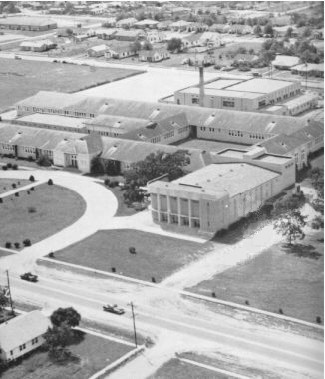
\includegraphics[width=0.5\linewidth]{images/SCP-001-the-foundation.jpg}
	\caption*{CA3的空照图,摄于最初发现后两个月。}
\end{figure}

\bb{UIU档案 0041:}位于██████, ██的变异高中校舍(Confirmed Anomaly 3,已确认异常3号)

\bb{项目等级:}53(高侵入性、未知能力、未知性质)

\bb{特殊收容协议:}\dd{已确认异常3号(CA3)需被高于30尺的带电铁丝网所环绕,并由美国陆军第█████排守卫。任何关于CA3内部的影像资料都需尽快删除,且所有目击者都将被无限期囚禁。}

在所有情况下都不允许人员进入CA3,或与居住其中的人员沟通。但在任何时候曾经进出CA3的人都应被囚禁与审问。

由于控制项目的一个或多个实体所拥有的未知能力,对CA3的直接军事突击已经被证实是不可行的。

\bb{笔记:}\ii{这是一份摘要,不包含所有关于CA3的资讯。对CA3的详细资料请参阅UIU档案0042至0218} - ██████主任

\bb{已知资讯:}特异事故处在1954年九月五日警觉到CA3的存在,当██████████高中的学生报告他们的校舍内部发生了前所未有的变化。

在发现的当下,CA3表现出数个-若非原本就存在的-异常性质:

\begin{itemize}
\item 设施内几乎所有墙壁都被钢筋混凝土所替换,某些房间则以其他材质建造,原因不明。所有对外的窗户都从内部被掩盖。
\item 所有课桌椅、个人财物、课本,或其他公立高中应有的物件都消失了。保险柜仍存在,但尺寸明显缩小,且是由不锈钢构成。
\item 所有房间与设施的格局、位置与尺寸都与学校原本的蓝图不符。且房间内部经常出现看似随机的修改,被改变的房间数量仍旧不明。
\item 发现了不少于七台的计算机,每一台都使用最先进的磁芯内存。在被分类为已确认异常之前,██████████并没有计算机。计算机内的所有资料都无法存取,且机器本身都被螺丝固定住。
\item 礼堂被大面的钢墙阻挡而无法进入。对这个阻碍进行搬移或破坏的尝试皆以失败告终。墙壁与礼堂本身的规模与用途不明。
\end{itemize}

一支被送入CA3内部以进行完整调查的小队(CA3-O5小队)没有返回,而负责寻找前一小队的第二支队伍也是(CA3-06小队)。该设施目前被封锁,等待新的收容措施。

\bb{更新:}在最初发现的二十三天后,守卫回报CA3发出「白噪声\footnote{\bb{译注:}White Noise,在各频率上功率都相等的“干扰”或者“噪声”}」,越接近礼堂噪声越大。五小时后,白噪声停止,但CA3内部能听见谈话声。

在深入调查之后,发现建筑内部现在包含了大量人员,所有人都看似漫无目的地在设施中游荡。值得注意的是,每个个体在外观上都与CA3-06的队员一致,但CA3内部的居民数目远超过CA3-06。囚禁或互动的试图因{[}机密]而失败。没有发现CA3-O5小队的十二名成员。此外,CA3的内部规划与前次调查也有明显差异。其中的运作机制尚未明了。

进一步的调查显示,大部分(或全部)产生出的物件本身都具有异常的性质。一部分的CA3-2开始看守这些物件(通称为CA3-3)或对其进行各种实验。

\bb{更新:}在前次调查的两天后,三名雷同的武装「守卫」出现在CA3的入口附近。由于这些守卫能无视伤害或武器等级地制服所有派往CA3的队伍,无法进一步探索建筑。

\bb{笔记:}在守卫出现前两天搜集到的报告指出CA3-2遵循标准UIU程序来处理礼堂中出现的物件。他们对UIU标准程序的知识与CA3-O5小队一致。

\bb{更新:}在UIU追踪CA6的过程中,两名与特工Dixon(CA3-06的成员)相同的人从路边的车辆中出现并强行掳走了CA6,将他拖入车中扬长而去。往后八个小时对车辆的追踪发现他们直接驶往CA3。在抵达的时候,守卫迅速开关前门让车辆通过。CA6没有再被寻获。

\hr

\hr

\bb{UIU档案0042:}CA3发出的讯息

1965年五月15日,以下讯息以摩尔斯密码发送至标准UIU通讯频道上。敏感资料已被删改,并将每个「句子」加以编排,讯息本身并未更动。

\begin{scpbox}

你好!我们是O5议会而且我们(控制、收容、保护)我们的行动已经为你们所知而且很高兴能做朋友。以前能当你们的一份子很好但最好是有更充足的资源(更多的资源)我们会控制住收容。我们对于守卫与囚禁的行为,在此表示诚挚的歉意,我们需要保障人员与秘密:同时也对时间上的延宕道歉,无线电讯号被一或二个SCP所阻挡。预期在短时间内会有扩张,因为我们需要礼堂以外的空间(尚可但不佳)

\end{scpbox}

八小时后,收到下列讯息:

\begin{scpbox}

扩张了!█████████联邦大楼现正运作中,需要博士守卫D人开始招募!寻找异常而且未来可能进行国际行动,研究当然可行;但跨国活动可能需要数周。此外我们O5都知道(抱歉没有O6)虽然很难探查,但媒介礼堂不是█████!再会并祝你们好运。

\end{scpbox}

更进一步的资讯参阅UIU档案0███:位于█████████, ██的变异联邦大楼(已确认异常10号)


\input{part00/001.thirty.six}

\chapter[SCP-001 Keter任务]{
	SCP-001 Roget - Keter Duty \\
	SCP-001 Keter任务
}

\label{chap:SCP-001.keter.duty}

\begin{figure}[H]
    \centering
    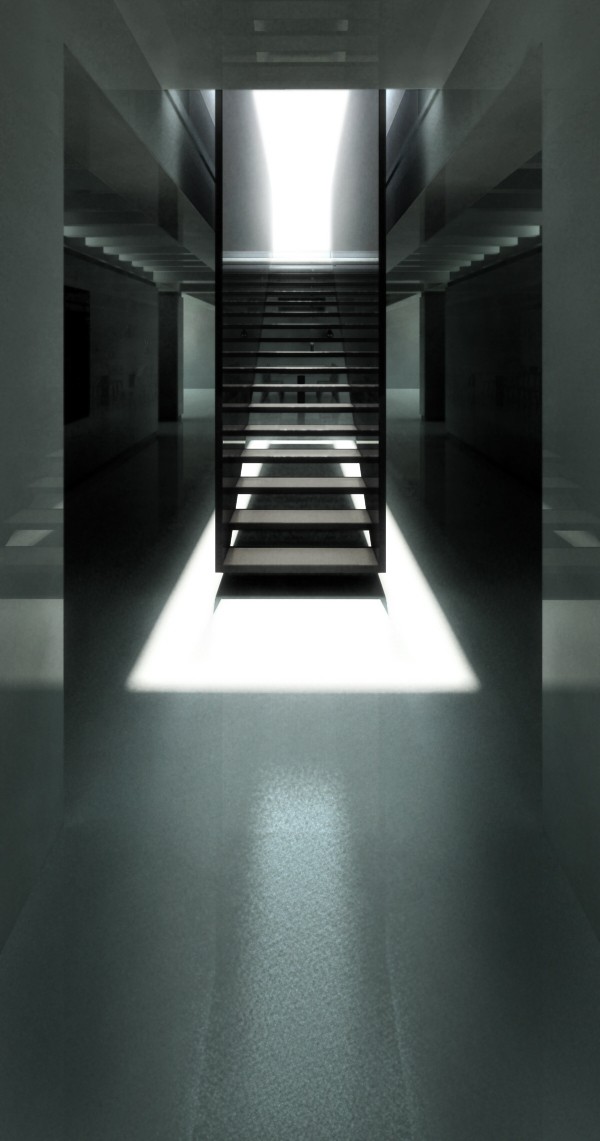
\includegraphics[width=0.4\linewidth]{images/SCP-001-keter-duty.jpg}
    \caption*{SCP-001的内部。}
\end{figure}

\bb{项目编号:}SCP-001

\bb{项目等级:}Thaumiel

\bb{特殊收容措施:}SCP-001的收容措施由监督指挥部制定,并作为单个收容措施统一执行。SCP-001内的各个收容单位皆适用一部分的收容措施。

指派于各收容单位的人员需各自分离,且只能拥有阅览各自收容文件的权限。若有人员阅读其他文件,或试图将SCP-001-K实体曝露于他人,需进行V级记忆删除并调离职位。

\begin{center}

\tred{存取SCP-001图样范例}

\tred{允许存取}

\begin{longtable}{|m{0.3\linewidth}|}
\hline
\multicolumn{1}{|c|}{SCP-001-K}\\
\hline
\endhead
\hline\multicolumn{1}{r}{\small{接下页}}
\endfoot
\hline
\endlastfoot
\raisebox{-.5\height}{
\includegraphics[width=\linewidth]{images/SCP-001-keter-duty-2.png}}
\end{longtable}

\end{center}

各收容隔间的门上都贴有一仪式化的标志,需即时维护。任何污损都会导致收容隔间逐渐消弱,直到收容循环无法持续。由于标志是以石材雕刻而成,维护应着重于预防风化以及外力破坏。

所有SCP-001-K实体都被收容于SCP-001中。只允许拥有六级权限的人员与SCP-001-K实体进行直接互动,而权限低于五级的人员则会授予伪造的收容文件。其他基金会收容的项目也将被归类为Keter以维持该等级的伪装。SCP-001-K实体不可被释放至SCP-001外,除非是在加速VK级现实重组的决议下。

若此一事件发生,六级人员将联系基金会人员以下达后续指令。

\bb{描述:}SCP-001是对所有被归类为Keter等级的异常项目的来源的代称,权限低于五级的人员仅能知悉这些项目的SCP文件。

SCP-001的设施位于{[}删除],高十一层楼并有四座翼楼。外观表现为一高大而无特色的研究设施。尝试详细记录SCP-001的外貌出现了矛盾不一致的报告。尝试绘制设施内部格局则产生相互冲突的楼层布置。目前观察到内部有宿舍、餐厅、娱乐区及办公区。收容隔间仅对五级以上人员开放。

目前已知存在有285个SCP-001-K实体。

SCP-001-K是所有源自SCP-001的异常项目的代称。在发现的当下,所有SCP-001-K实体都被收容于SCP-001中,但迄今已有部分遗失。每个SCP-001-K实体都与另一个能相互抵销异常效应的实体收容在一起。

当任两个SCP-001-K实体之间的收容循环被破坏时,收容隔间将发生局部性的异常现象。收容隔间内的物理法则将会改变,以符合所有未收容的SCP-001-K实体的异常效应,此现象包括但不限于触发此异常的实体。

SCP-001最早由二次大战后驻扎于希腊的美国陆军所记录。当异常性质被发现后,数个组织立刻宣称自己拥有此地的控制权。由于若干SCP-001-K实体遭到释放,迄今仍无法复原这段时期SCP-001的收容资料。

\begin{longtable}{m{0.3\linewidth}m{0.6\linewidth}}
\hline
被指定为SCP-001-K的项目 & \multicolumn{1}{c}{收容方式}\\
\hline
\endhead
\hline\multicolumn{2}{r}{\small{接下页}}
\endfoot
\hline
\endlastfoot
\hyperref[chap:SCP-718]{SCP-718},\hyperref[chap:SCP-689]{SCP-689} & 数个SCP-718被放置于木乃伊化的人体上,以SCP-689为中心围成一三角形。所有实体会不定期地转开视线,导致SCP-689出现在其中一个人体并消灭SCP-718,造成更多SCP-718的产生。此时其他SCP-718会恢复观察,迫使SCP-689回到原本的位置。\\
\hyperref[chap:SCP-990]{SCP-990},\hyperref[chap:SCP-122]{SCP-122} & 数个SCP-122实体被观察到以身体阻挡外界的声音与光线,并在SCP-990的身边念床边故事,以确保后者在物理世界中持续沉睡。\\
\hyperref[chap:SCP-1178]{SCP-1178},\hyperref[chap:SCP-1984]{SCP-1984} & SCP-1178悬浮在立方体房间中,SCP-1984紧追在后。目前已知有六种不同的追赶方式作随机更换,SCP-1984被观察到距离SCP-1178至少15公尺远,只要SCP-1984加速,SCP-1178也跟着加速。收容人员目前正研究如何减轻SCP-1178被SCP-1984引爆时产生的伤害,并防止它摧毁其他SCP-001的收容设施。\\
\hyperref[chap:SCP-1440]{SCP-1440},\hyperref[chap:SCP-836]{SCP-836} & SCP-1440被铐在一宽敞圆形房间的门上,周围的建筑结构被SCP-836影响而不断朝SCP-1440靠近,并被项目的异常性质摧毁。SCP-1440表示他被一位神父所囚禁,除此之外没有其他相关资讯。\\
\hyperref[chap:SCP-1048]{SCP-1048},\hyperref[chap:SCP-1055]{SCP-1055} & SCP-1048持续地剥下SCP-1055新生的物质来建构新的实体。SCP-1055不断移动,并摧毁靠近的SCP-1048。这些残骸又会被制造成新的SCP-1048或用来修补其他实体。目前隔间内估计有████只SCP-1048,而隔间的容量估计是██████████只。\\
\hyperref[chap:SCP-1295]{SCP-1295},\hyperref[chap:SCP-871]{SCP-871} & 一个服务生装束的金发女性人类\footnote{似乎是SCP-001的一部分}不断为四个SCP-1295实体送上SCP-871,她从一张木桌上持续拿取SCP-871并端给SCP-1295。四个实体都在抱怨菜单单调,但称赞SCP-871的品质与种类。\\
\hyperref[chap:SCP-505]{SCP-505},\hyperref[chap:SCP-140]{SCP-140} & SCP-505被悬挂在SCP-140上方,以70,000字\slash 15分的速率写下关于Daevite文明与文化的信息\footnote{以希腊字母写成。}。由于SCP-505叙写的文字已经超过目前的时间达七十年,中断此循环可能会导致人类历史全面而不可逆的改写。\\
\hyperref[chap:SCP-231]{SCP-231},██:██-N & {[}删除]和一已遭消灭的异常项目的剩余互动。收容迄今,除了六次潜在的失效以外,110-蒙托克程序已成功预防这种互动所产生的XK级事件。为了阻止VK级事件而采取的蓄意失效已提交监督指挥部审理中。\\
\hyperref[chap:SCP-058]{SCP-058},\hyperref[chap:SCP-1983]{SCP-1983} & SCP-058被悬挂在一圆洞上方,洞中放满了仍在跳动的人类心脏。SCP-058的内部和周围塞满额外的心脏组织。SCP-1983实体不断从房间昏暗处试图将组织从SCP-058身上扯下,SCP-058一面击退它们,一面从洞中同化更多心脏组织。\\
\hyperref[chap:SCP-682]{SCP-682},\hyperref[chap:SCP-296]{SCP-296} & SCP-296内的实体皆为人形,特征符合在维持项目收容时死亡的人员。SCP-682无法伤害这些人形,时而狂暴地试图杀死它们,时而畏缩在收容隔间的中心。当Dr. ██████ █████████问起时,SCP-296表示SCP-682获判有罪,因此处罚其不得杀人或自杀。\\
\hyperref[chap:SCP-579]{SCP-579},\hyperref[chap:SCP-055]{SCP-055} & 圆榫打不进方洞。
\end{longtable}

\bb{附录001-A:}

\tred{需要六级权限}

\tred{允许存取。欢迎,监督者。}

\begin{scpbox}

找回来了么?

我们能看到彼岸,人事已非,但我们也在进步。

提案是最新的紧急命令,所有K级项目的研究立刻中止,并以收容而非传播的原则重新进行。灾难已经带走太多人命了,该让事情回到

\{\{

清洗行动已经大幅扩大,Olympia中的项目皆已完全收容,感谢红色使我们能够长期预防任何事件发生。在你之中可以找到更多关于收容策略的信息。笑一个吧。

事情正逐步改善。我们已经让色彩重新运作,我听说他们不久之后也会把人们的知觉取回。如果你看到第七新娘,请表达我对于她打开盒子一事的遗憾,或许她会记得。

\end{scpbox}

\bb{附录001-B:}VK级现实重组是当所有SCP-001-K实体皆从收容循环中被释放时,理论上会出现的异常现象的代称。如果所有SCP-001-K实体都被释放了,这个效应将改变已知的宇宙,使其在一无异常的物理法则下运作。目前正在研究基金会如何适应这种变化以及如何保护新宇宙和当下的现实。


\chapter[SCP-001 孩子们]{
	SCP-001 djkaktus - The Children \\
	SCP-001 孩子们
}

\label{chap:SCP-001.the.children}

\newcommand{\vdotsc}[1]{\cl{\multido{}{#1}{. \\}}}

\begin{scpboxbbwmc}
\GG{\wred{\bb{警告:以下文件被分类为}}}

\Hg{\wred{\bb{5级}}}

\GG{\wred{\bb{此分类由监督者议会授权}}}

\g{\bb{任何未经5级授权试图访问该文件的行为将被记录,并且查阅者将被处决。}}
\end{scpboxbbwmc}

\hr

\vdotsc{7}

\begin{scpboxc}
输入五级基本安保证书
\end{scpboxc}

\vdotsc{7}

\begin{scpboxc}
Command:\textbackslash users\textbackslash O513>\_ 6110298-父罪与子罪-3561840
\end{scpboxc}

\vdotsc{7}

\begin{scpboxc}
允许访问,初级模因抹杀剂解除,晚上好,O5-13。
\end{scpboxc}

\vdotsc{7}

\begin{scpboxc}
警告:此文档部分内容已被锁定。
\end{scpboxc}

\begin{scpboxc}
解锁需要额外的5级权限。
\end{scpboxc}

\vdotsc{7}

\hrule

\begin{figure}[H]
	\centering
	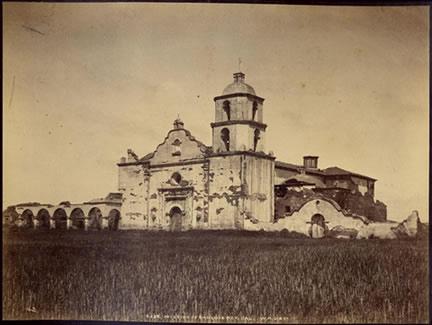
\includegraphics[width=0.5\linewidth]{images/SCP-001-the-children.jpg}
	\caption*{位于墨西哥圣马可的San Marcos de la Vida Eterna教堂,\\ 照片上的日期为07/27/1903}
\end{figure}

\bb{项目指定编号:}Item-001

\bb{收容等级:}Keter-Thaumiel

\bb{收容状态:}激活-稳定

\bb{收容措施:} 物体-001(Item-001)现在正被收容于墨西哥的圣马可,收容地点位于San Marcos de la Vida Eterna教堂的旧址地下。原始收容措施已经证明可以有效收容物体-001。收容区域现在被指定为一个高安保级别的军队废物处理厂,墨西哥法律则禁止所有平民接近该站点10km范围内。围绕物体-001的收容区域将有自动化闭路监控无人机进行巡逻,并且这些无人机被设计为一旦见人将格杀勿论。

\bb{O5备忘录001-Alpha:}\ii{对于有关SCP-001,也就是前物体-001,的所有信息收容将成为最高优先事项。我已经授权将资料库之中相关资料清除,并在原地址上创建数个错误项目。如果真的有人能追查到那个地址,那些伪装项目也足够让他们感到失望了。我现在抽出了好几个EX的SCP项目放置在那个地址上,直到我们找到更好的伪装项目为止。}

\ii{删除你找到的任何信息,堵住任何可能的漏洞,将这些信息掩埋在你觉得足够多的模因抹杀剂之下。要做到这一点,你需要做比完全删除资料还要多的多的工作。-O5-2}

\bb{项目描述:}物体-001是对9名人类组成的群体的指称,这些人年龄在4-11岁不等.他们因为001项目:“神之双子”(Twins of God)(见项目提案001以获得更多信息)而取得了异常性质。因为对物体-001进行了不当使用,导致了一名高级人员的死亡,这也使得对其进行处决变得必要。作为这一事件的结果,物体-001现在按照现有收容措施进行了收容。所有9名物体-001的个体都在功能上已经进入了脑死亡状态,但却仍然表现出生命体征,而不论对其的收容措施情况如何。

物体-001的个体都放射出大量的伽马射线,放射量通常都在███GJ以上,并且以一种独特的形式进行变换。当每个个体单独收容时,这种放射模式似乎是随机的,但如果将这些个体进行集合收容时,这些放射模式似乎会出现某种确定的特征。因此,每一个个体之间收容间隔大约应保持在████。另外值得注意的是,物体-001的个体是具有辐射发光性的。在这些个体进入激活状态时,对它们进行视频监控是不可能的,因为在此状态下的个体出现在屏幕中时将导致录影脚本发生损坏。

当一个物体-001个体与其他个体之间相隔小于20m时,它将表现出对物体、人类个体或是某块区域的远距离毁灭能力。对于此性质将会稍后在此文档之中进行详细描述。

根据监督者议会的命令,物体-001被分类为一个Thaumiel\footnote{"Humphrey, W., Lemke, R., Christian, K., Roesler, J., \& Kaiser, N,(1920),《收容分级提案:Thaumiel》,基金会研究出版社,2(7)。"}-Keter实体。

\vs\hrule

\begin{scpboxbbwm}
\bb{警告:}有关物体-001的更多信息已经锁定,并且已经被分类为5级。模因抹杀剂已经插入其中保证有关于物体-001的信息不会出现外泄。非监督者议会成员,并且不具备5级模因抵抗条件的人员将会受到模因抹杀剂影响而被处决。\bb{\ii{你已受到警告,并且这是最终警告。}}
\end{scpboxbbwm}

\cl{\bb{项目提案001: 锁定}}

\cl{\tred{+ 输入授权密码}}

\cl{\tred{1485992-13人乘死者船-4910581}}

\begin{scpboxc}
{[模因抹杀剂无效化]}
\end{scpboxc}

\begin{scpboxbbwm}
\GG{\bb{\tred{项目提案:“神之双子”}}}

\Gg{研究团队:Omega-5}

\g{\bb{项目日期:02/13/1922}}

\Gg{\bb{目的阐述:}}

\ii{此项目旨在创造出一个异常实体,该实体能在基金会中心高层必要的掌控之下,对基金会及全球安全造成威胁的敌意异常个体加以远距离摧毁。}


\bb{研究团队主任:}Dr. ███ █████,Ph.D.(O5-1)

\bb{副主任:}████ ██████ (O5-2),████ ████(O5-3)

\Gg{\bb{项目需求:}}

\begin{itemize}
	\item 取得并且使用物体-███:“亚原子加速系统”。
	\item 取得并且使用物体-███:“Harken之门”。
	\item 取得并且使用物体-███:“多重注射器”。
	\item 能够制造必要收容措施和研究设施的材料。
	\item 不少于50名成年人类个体(D级)作为测试目的之用。
\end{itemize}
	
\Gg{\bb{项目细节:}}

通过分析最近从物体-███和物体-███实验之中取得的信息,一个之前不可能出现的机会摆在了基金会面前:一种能力,能够穿越远距离改变物体量子组成,从而导致该物体从功能上不复存在\footnote{Maxwell, T., \& Gouram, A.(1927),《远距离上的量子性质》,基金会研究出版社,05(02),213-230页。}的能力。到目前为止,通过使用物体-███来改变人体性质从而对这一效应加以更大的操控,我们认为这一点是可以做到的。为了达到我们的最终目的,物体-███、物体-███和物体-███已经从基金会记录之中抹消了,并且它们将会单独收容在这个项目最初的研究设施之中。

在美国核试验设施的幌子之下,我们将在墨西哥北部建立一个站点,远离人群,这也是出于对这一理论进行安全测试的考虑。为了将这些实验对自然性质可能造成的潜在影响降到最小,我们将对这一项目进行最高的防护措施,对灾难性收容失效事件也建立了数个意外保险措施。这些保险措施将会在下面列出。

如果这一项目最终成功,这些实验创造的实体,暂时指定为物体-001的控制权,将交由基金会管理者掌控来对抗我们指定为GOI-003“地狱王国”(Kingdom of Abbadon)的异常敌对组织,一系列心灵抹杀剂将植入这些实体之中,对于这些抹杀剂的取得也只对管理者单独开放,这是作为确保这些个体不会落入敌对组织控制之中的保险措施。

\end{scpboxbbwm}

\begin{scpboxc}
{[模因抹杀剂无效化]}
\end{scpboxc}

\begin{scpboxbbwm}

\GG{\bb{意外保险收容措施:}}

\bb{Alpha:} 当出现灾难性收容失效事件时,植入这些实体之中的心理抹杀剂将启动,将其处决。每一种抹杀剂都被赋予不同的优先级并且应按顺序使用,以下是优先性列表:

\begin{itemize}
	\item Berkeley剂:降低身体活动能力。
	\item Anastasia剂:降低异常性质[正在开发中]。
	\item Nezbit剂:降低心理能力。
	\item Orion剂:对高级神经系统的全面化学性溶解。
\end{itemize}

\bb{Beta:} 在Alpha保险措施失效的情况下,安保人员应前去处决物体-001。将这些个体捕获的可能性不大,也不推荐这么做。建议相关人员与物体-001个体之间保持安全作业距离,并且穿着必要的基金会开发的反辐射防护装甲。同时推荐进行远距离弹道射击,因为这一行动将不会那么快吸引物体-001个体的注意。

\bb{Delta:}在Beta保险措施失效的情况下,基金会控制的长距离弹道武器将启动并且直接作用于物体-001个体上。我们将在研究设施外建立一个10km的边界,不少于10架重装轰击加农炮部署于这一边界上。在Delta措施启动时,它们将用于处决物体-001。

\bb{Epsilon:}在Delta保险措施失效的情况下,站点自身装载的自爆装置将启动,基金会管理者将全程监督Epsilon措施的实施情况。

\Gg{\bb{项目批准:}}

\begin{figure}[H]
	\captionsetup{singlelinecheck=false}
	
\includegraphics[max width=\linewidth]{images/SCP-001-the-children-2.png}
	\caption*{\ii{基金会管理者R. D. Fritzwilliams}}
\end{figure}

\begin{figure}[H]
	\captionsetup{singlelinecheck=false}
	
\includegraphics[max width=\linewidth]{images/SCP-001-the-children-3.png}
	\caption*{\ii{项目主任O5-1}}
\end{figure}

\end{scpboxbbwm}

\cl{\bb{项目报告001-Delta: 锁定}}

\cl{\tred{+ 输入授权密码}}

\cl{\tred{- 7483529-九分钟后午夜-1889475}}

\begin{scpboxc}
{[模因抹杀剂无效化]}
\end{scpboxc}

\begin{scpboxbbwm}

\GG{\bb{\tred{项目“神之双子”进程报告}}}

\Gg{研究团队:Omega-5}

\g{\bb{项目日期:04/18/1924}}

\bb{进展细节:}

对于新物体-001个体的收容立刻就出现了问题,因为在约35\%活跃项目人员之中产生的[从记录之中删除]和急性放射病,我们出现了█人伤亡。对于收容措施的调整变得很有必要,以及这个现在我们指定为站点-001的站点内部结构也进行了强化。人员的住所已经后撤到了一处里主要研究设施有5km远的地方。

在苏丹,一次由地狱王国主导的对基金会设施袭击再次加剧了对远距离防卫系统的紧急需求,也同时加快了激活物体-001的时间表。在基金会管理者的命令下,我们得到了额外的物资来发展更为高效的实验设施。

另一件核心要件则是如何将异常性质收容在一个人类个体之中。在所有100\%的实验个体之中,尽管异常性质都只出现了一些小事故就能收容在他们体内,但所有的实验个体都会立刻瘫痪并且出现严重的脑溢血。而异常性质发挥效用的唯一证据则是站点结构或人员的随机突发毁灭,理论认为这一现象是因实验个体心理控制力恶化,无从控制这些异常性质而导致的。在所有100\%这些情况下,我们都启动了心理抹杀剂来将这些前物体-001个体处决。

站点外人员主导的另一项实验给了我们灵感,或许将这种异常性质平均分散到数个人类个体体内是可能的\footnote{Enjilian, M., \& Johnson, R.(1923)《数个Keter项目的异常性质》,基金会研究出版社,1(11)。},如此一来异常性质对人类个体心灵造成的压力问题将得以解决\footnote{Everly, K., \& Everly, J.(1922)《被消灭的Keter实体的大脑结构:对超自然个体认知结构的进一步分析》(第三版,第一章,自费出版,145-178页)芝加哥,IL:基金会科学出版社。}。

在一次使001号站点运转能力降低的测试,以及在基金会管理者命令下将D级人员转出站点到其他课题的行动之后,我们不得不讨论项目是否能继续进行这一问题。在与17号站点的主任进行咨询之后,一队武装特工进驻了墨西哥圣马可的San Marcos de la Vida Eterna教堂,并且他们还找来了一群年轻人进行测试。我们对圣马可城全体市民都进行了A级记忆消除,而这些人则之后被转送到了09号站点以备下一步之用。圣马可城本身则成为了新的001测试站点,23名最健康的个体被挑选出来进行实验,而剩余个体则全数处决。

\end{scpboxbbwm}

\begin{scpboxc}
{[模因抹杀剂无效化]}
\end{scpboxc}

\begin{scpboxbbwm}

\Gg{现状:}

现在这个项目准备进入下一阶段,下一阶段的实验将会在新的001测试体上进行,这一实验还在等待来自中央控制层的命令。以下这封信是申请将项目推进到下一阶段的,内容如下:

\begin{scpbox}

04/03/1924\\
致:基金会管理者\\
自:Omega-5团队负责人

管理者Fritzwilliams:

正因为从您办公室之中发出的每一条缩减预算和削减补给的命令,我们的项目随着每一条这种命令的发出而越来越难以保持进度。在中央控制层还没有主动与我们进行联系的情况下,我们只能认为对我们的指示是不变的。

一份为帮助我们项目尽快获得结果而寻求物资帮助的申请很快也会到达您那里,我们希望您能看到形势的变化,并且给我们的一个良好的答复。如能及时回信,不胜感谢。

███ █████\\
项目负责人

\end{scpbox}

04/15/1924\\
致:Omega-5团队负责人\\
自:基金会管理者

█████:

我们给你下达的指令依然没有改变。如果你们的项目能够成功,那么我们就大可高枕无忧了。但很不幸的是,严酷的事实时刻提醒着我们,我们身陷一场战争之中,而物资又是如此贫乏。为了保证我们事业的隐秘性,我们再没有面对过比这状况更严峻的时期了,更不要谈继续你们的研究。但我仍会尽我一切努力帮助你们,不为别的,只因为你们的研究能从地狱王国手中保护我们。

我已经接到了你们的申请,尽管从道德上我没有任何理由去批准它,但我作为基金会领导者还是强迫自己批准了它。市民随便你们挑,但只允许挑成年人,也不要肆意践踏无辜者的生命。上帝知道,为了我们的目的已经有足够多的无辜者鲜血洒下了,我不希望再看到更多。

管理者Fritzwilliams\\
基金会中央管理层

\end{scpboxbbwm}

\cl{\bb{文档:GOI-3“地狱王国”: 锁定}}

\cl{\tred{+ 输入授权密码}}

\cl{\tred{- 4561273-影覆沙丘-0948390}}

\begin{scpboxbbwm}

\GG{\bb{\tred{同行组织文档003}}}

\Gg{\bb{指称:地狱王国(Kingdom of Abbadon)}}

\bb{威胁等级:}非常高\\
\bb{活跃等级:}非常高\\
\bb{优先度:}5级

\bb{综述:}GOI-003“地狱王国”是对一群异常敌对人性个体的指称,他们现在位于撒哈拉沙漠的某处,该处根据其手稿之中的描述被称为“吾等神王Abbadon之城”。这些人形个体从很多方面都与人类相似,但他们所有成员都至少是I级现实扭曲个体。\footnote{Benson, R.(1921)《现实扭曲个体分级》,基金会研究出版社,3(7),10-58页。},同时高级个体已经达到了III级或者IV级的现实扭曲分类。由于他们本身异常性质之强烈,对它们的捕获和收容是不可能的,并且任何这方面的尝试都十分危险。

\bb{最初发现:}GOI-003最初是由法国军队人员于1912年,对一起利比亚北部村落的袭击行为调查之中发现的。军队的护卫队遭到了袭击,80\%的人员死亡。幸存者称他们被不多于6个人的“巫师们”袭击了,这些“巫师”能进行飞行,并且可以抵挡枪械攻击。这些幸存者,以及可能的目击者都被给予了记忆消除之后释放了。

基金会人员最早遭遇GOI-003人员是在一次对埃及南部破碎之神教会仓库的袭击尝试之中,就在那次行动之中,机动特遣队Alpha-4“无疆”(No Borders)被一群与法国军人描述一致的异常个体袭击。机动特遣队Alpha-4成功击退了它们,并捕获了一名低级成员。在对这名俘虏进行处理和审讯之后,基金会知晓了“地狱王国”的本质,中央管理层开始采取措施保证基金会不受到这个异常组织的侵扰。

根据收集到的数据,“地狱王国”原本只是一个阿拉伯半岛现实扭曲者组成的团体,希望在撒哈拉的不毛之地之中开辟属于他们自己的国家。由于他们本身所具有的异常性质,他们可以将严酷的地形变为他们所需要的,同时利用这种地形确保侵入者远离他们的国家。随着时间的推移,他们的数量随之增加,新生儿将被带到国家的统治者“Abbadon神王”面前转变为现实扭曲者。

但是,由于成员之间的近亲婚育和基因障碍对他们社会产生的毒害,地狱王国本身变得十分脆弱,并且在20年内就难以作为一个独立的组织存在。收集的数据显示地狱王国自身已经知晓了这一点,并开始展开行动防止这一未来的发生。到目前为止,基金会部署在非洲大陆内部及其周边的许多设施都已经遭到了该组织激进成员的攻击,基金会为此付出了不少于75条人命的代价,并且至少有12件异常物体被偷走。

\bb{结论:}因为对抗地狱王国成员这一行为本身的难度和危险性,同时也因为对他们的行为缺乏情报,不建议任何人员在缺乏重型武器部队时与地狱王国成员发生冲突。对抗地狱王国手段的研究现阶段正在进行中。

\end{scpboxbbwm}

\cl{\bb{备忘录001-Alpha:锁定}}

\cl{\tred{+ 输入授权密码}}

\cl{\tred{- 7105922-无情神明之眼-0981478}}

\begin{scpbox}

\bb{日期:}11/29/24\\
\bb{用户:}Omega-5-1\\
\bb{主题:}001

就这样,我们做到了。我们做到了不可能的事情。我们狠狠打了神一耳光并且把他的冠冕抢到了我们手上。

这是一个新的充满荣耀的日子。

5有关于将异常性质平分到一个集体之中的看法是对的。在之前的实验体之中,尽管我们已经尽我们所能加固他们的身体,但注入他们身体的总计███的能量还是太多了。我没法告诉你那些D级人员的数量,那些我们只能看着他们的皮肤从他们的骨头上融化,他们的骨头碳化之后如同尘土飞散,最后我们不得不把他们从地上铲走的D级人员。几十名?几百名?我不知道。比我们期望的多得多,也比基金会可以容忍的要多的多,即便是我们这样的项目之中。

13对我们在墨西哥所做的一切表示遗憾,但13是短视的,管理者也是短视的,一些人的死亡,甚至是许多人的死亡,与防止世界被毁灭较之如何?一文不值。那些孩子们现在已经是神了,他们的生命是为了一个更崇高的目的而存在的。还有什么生命,能比得上全知全能呢?

明天即将开始实验,你听得到吗?

\end{scpbox}

\cl{\bb{项目报告001-Delta: 锁定}}

\cl{\tred{+ 输入授权密码}}

\cl{\tred{- 7483529-九分钟后午夜-1889475}}

\begin{scpboxc}
{[模因抹杀剂无效化]}
\end{scpboxc}

\begin{scpboxbbwm}

\GG{\bb{\tred{项目“神之双子”进程报告}}}

\Gg{研究团队:Omega-5}

\g{\bb{项目日期:01/17/26}}

\bb{进程报告:}

现在,9名被集合指定为物体-001的个体已经被收容于一个进行过加固的仓库之中,并且在测试站点01进行试验。这些个体在执行指令而启动时,没有表现出高级脑部活动的迹象。尽管如此,这些个体整体能够对信息进行处理,并且能以在对其进行的每个个体模因循环控制的过程中加入信息的方法加以控制。

所有这些个体现在都是V级辐射活跃危害元,人员禁止在没有穿着抗辐射装甲的情况下进入物体-001周边1km以内。每个个体之间放射伽马射线的模式是随机的,但当他们聚集到一起的时候,他们的辐射模式变得类似于一名清醒人类在脑电波扫描器(EEG)上表现出来的脑波模式。但尽管有所相像,比起正常人类的脑波模式,这种模式更具有随机性和不一致性。

物体-001整体能够共同引导一种来自于我们未知的地外空间的庞大能量,并且能够运用这一能量在量子层面上将分子分解。这一性质使得它们可以在任何距离上将任何物体不为人知地加以歼灭,只要这一物体的特征和所在地点对物体-001进行了一定程度上的详细描述。

以下是物体-001于01/17/26的测试结果:

\hr

\bb{测试序列023}\\
\bb{对象:}物体-001\\
\bb{研究团队:}Omega-5

测试目标:确定物体-001效应的最远边界

\bb{第1轮:}测试物(钢条)放置于物体-001 5km远处。物体-001被操作者(███ █████博士,Omega-5负责人)下令摧毁目标物体。

\bb{结果:}测试物体在物体-001收到指令并且执行之后不久被消灭。与测试之前相比,目标物没有任何质量留存。

\bb{第5轮:}测试物(钢条)放置于物体-001 800km远处。物体-001被操作者(███ █████博士,Omega-5负责人)下令摧毁目标物。

\bb{结果:}测试物体在物体-001收到指令并且执行之后不久被确认消灭,距离对于这一效应而言没有影响,更远距离的测试将加入下一序列的实验之中。

\ii{这些孩子如设计好的一般对命令加以了执行,我对他们在时机成熟之时成功执行使命毫无怀疑。他们毫无动摇,毫无感情,同样也不可摧毁,在跨越宇宙将死亡降临之前也仅仅只需要一个命令而已。诚然,这就是为人类之中最刚毅者设计的武器。 - O5-1}

\hr

\bb{测试序列025}\\
\bb{对象:}物体-001\\
\bb{研究团队:}Omega-5

\bb{测试目标:}确定远距离摧毁时物体大小的上限以及下限

\bb{第2轮:}测试目标(铁球,直径3m)放置在距离物体-001 1000km的位置,物体-001被操作者(███ █████博士,Omega-5负责人)下令摧毁目标物。

\bb{结果:}测试物被消灭,如同预想一般

\bb{第3轮:}测试目标(破碎之神教会的工坊,位于土耳其的███████████)距离物体-001 11500km,物体-001被操作者(███ █████博士,Omega-5负责人)下令摧毁目标物。

结果:目标被消灭,在其周边区域没有发现额外的损伤。这一事件的目击者被给予了A级记忆消除并且释放拘捕以进行额外的实验。测试显示这些个体,或者这一个群体需要精确指定目标,仅仅指定某一个地区不足以让它们进行消灭。

\bb{第7轮:}测试目标(成年男性,33岁)距离物体-001 11500km,物体-001被操作者(███ █████博士,Omega-5负责人)下令摧毁目标物。

结果:目标被消灭

\end{scpboxbbwm}

\cl{\bb{收集的相关基金会通讯及通知: 锁定}}

\cl{\tred{+ 输入授权密码}}

\cl{\tred{- 0002481-警惕之眼-4781621}}

\begin{scpboxc}
{[模因抹杀剂无效化]}
\end{scpboxc}

\begin{scpbox}

\bb{日期:}02/01/26\\
\bb{致:}Omega-5团队负责人\\
\bb{自:}管理者Fritzwilliams

我已经知悉你们在001项目上大获成功的好消息,我完全无法描述这一成功是多么重要。我们终于可以将地狱王国画上一个句号了,并且在未来,我们将能更好地保护自己。在这一刻,我对你们的工作致以永恒的感激。

但,我必须明确提出对你的忧虑,O5-1。尽管你取得了重大成功,但最近你的来信让我烦心。我对你是Omega队的最佳领袖这一点毫无怀疑,但我还是觉得这一成就的压力是否在你的身上造成了某种代价。我知道自己已经为此付出了代价。不论如何,只要这一切结束,我准备将你提拔成为新建的19号站点的主任,当然,这会是在你进行足够的休息重新恢复过来之后的事情了。在下个月我和你的会面时刻我们可以详谈此时,到时候我们已经把地狱王国的一切都安排妥当了。

你真诚的

管理者Fritzwilliams

\end{scpbox}

\begin{scpboxc}
{[模因抹杀剂无效化]}
\end{scpboxc}

\bb{日期:}02/14/26\\
\bb{致:}基金会中央管理层\\
\bb{自:}Omega-5团队负责人\\

我很好,管理者。这个项目已经完成了,你到来的时候我们就能完成我们的使命了。

\ii{1}

\begin{scpboxc}
{[模因抹杀剂无效化]}
\end{scpboxc}

\begin{scpboxbbwm}

\Gg{全员通告:全人员}

\Gg{[由监察者命令编辑]}

\Gg{\bb{由基金会中央管理层发布}}

\bb{日期:} 03/21/26\\
\bb{主题:}管理者Frizwilliams

基金会管理者R. D. Fritzwilliams已经遭到谋杀。我们已经发布了一份全基金会通缉令以缉捕杀害他的凶手及其帮凶:███ █████博士、████████ ████博士、████ ██████博士、█████ ██████博士以及██ ████特工。我们认为这些人员持有武器并且十分危险,并可能持有一个高危异常物体。如果你手上有任何有关于这些人员所在地信息,请直接向站点主任报告。

我们已经成立了一个临时管理议会,主要成员由Omega-5团队的高级指挥人员组成,这一人事任命是由已故的管理者下达的。这一议会将会持续监督基金会行动,直到我们能选出一名新的管理者为止。

\end{scpboxbbwm}

\begin{scpboxc}
{[模因抹杀剂无效化]}
\end{scpboxc}

\begin{scpboxbbwm}

\Gg{全员通告:全人员}

\Gg{\bb{由基金会中央管理层发布}}

\bb{日期:} 03/22/26\\
\bb{主题:}对GOI-003调查队的解散

\bb{通知:}\ii{我们认为以下机动特遣队调查队已经处于无行动状态,这些机动特遣队人员应向17号站点主任进行报告:}

\ii{机动特遣队Alpha-1:“王的侍从”(All The King's Men)}

\ii{机动特遣队Alpha-2:“地球之盐”(Salt of the Earth)}

\ii{机动特遣队Alpha-3:“哈佛男孩”(Havard boys)}

\ii{机动特遣队Alpha-4:“无疆”(No Borders)}

\ii{机动特遣队Alpha-5:“兄弟羁绊”(Band of Brothers)}

\ii{机动特遣队Alpha-6:“黑暗证言”(Dark Testimony)}

\end{scpboxbbwm}

\begin{scpboxc}
{[模因抹杀剂无效化]}
\end{scpboxc}

\begin{scpbox}

\bb{日期:}11/01/26\\
\bb{致:}监督者议会\\
\bb{自:}23号站点主任Harrison\\
\bb{主题:}23号站点勘探报告

我的手下带着报告回来了。我将现场照片随信附上,但我还是无法相信着一切。什么都没有了,只有永恒不变的沙漠。就像他们从没有出现在那里过一样。

我让他们仔细检查,你们是对的,没有留下任何尸体。不过本来那里也就该什么都没有,不是吗?

不论如何,我不知道你们被迫和魔鬼做了怎样的交易,但谢谢你们。

\ii{-Harrison}

\end{scpbox}

\hr

\vdotsc{14}

\begin{scpboxc}
你已经三分钟没有操作这个终端了,你需要帮助吗?
\end{scpboxc}

\vdotsc{14}

\hrule

\bb{新语音文件:}

\tred{► 开始录音}

\tred{❚❚ 暂停录音}

[开始录音]

我觉得这是该干这事情的时候了,趁我还能记得一切的时候早早干了比较好。距离我读这篇文档已经过去很长时间了,这时间长得可以追溯到'26年的那个晚上。距离人们可能知道我们所作所为的真相,到底在地狱王国、O5-1和管理者身上发生了什么事情已经过去太长的时间。该死。如果这一切都已经掩盖在记忆消除之下,那么我可能是最后剩下的一个了。

我绝不会把这一切带进坟墓里的,至少这一件事绝对不会。

一总是有着超凡魅力,这一点在各种记录上已经描述得够多了。这就是为什么Fritzwilliams给了他Omega-5团队管理者的身份,把他置于二之上,即便二在基金会里待的时间比一要长得多。这并不是说一并不聪明,恰恰相反,他是我一起共事过的最杰出的研究者之一,就算过了这么久也是如此。他写作了所有Omega-5团队研究的报告,在我们离一个成熟的队伍还远着的时候他就已经这么做了。在当时我们只是17号站点初级研究员之中的一小群而已,而他,雄辩、热情而又\ii{偏执}。

他又是那么超然。他爱着他的事业,请不要误解我,研究对于他而言是最高的愿望。但对于基金会的指示,或者是有关收容带来的压力,他一点兴趣都没有。他多次对我说,我们没有充分利用资源。如果我们不是那么害怕这些异常物品,我们本可以对他们进行更好的收容的,但我们就是害怕用一些异常物品去收容另一些的方式。当然,也是他,是Thaumiel级别的最初分类设计者,他和Epsilon-2队伍完成了这一编级。我想,这或许是他为何对抓住机会参与到我们在001项目之中的工作之中如此热忱的原因。

001项目,那是如此地超凡脱俗,前所未见,但同时,地狱王国也是如此。记录在这里的文档连它特别之处的一半都无法描述,而其他的部分都已经散佚在历史之中。在地狱王国面前,我们与之相较简直就是疯狂而滑稽。一群得到了庞大资金支援的科学家和武装部队,对阵一小群绿型个体(type-green)的军队,我们甚至都不知道他们的弱点在哪里。II级和III级能做到的事情,已经远超出我们所能办到的,这事情还发生在我们见到第一个斯卡兰顿现实稳定锚半个世纪之前。一些报告称他们的统治者是个V级。如果那是真的,只要他想,眨眨眼睛就能把我们从地图上抹掉。

在1922年整一年之中,地狱王国一个组织要单独为所有基金会站点的摧毁事件负责。当然,这些事件不仅仅发生在撒哈拉沙漠周边的非洲地带,只是我们从没有公开过而已。地狱王国的活动范围北至直布罗陀,南至马达加斯加。他们暴力闯入站点,毁掉一切,只带着一些物品离开,当然也不忘删掉所有记录。那我们当时在干什么?我们才刚刚开始分类现实扭曲者,更不要说如何和他们战斗了。如果地狱王国对欧洲或者中东的一个更大的站点发起这样的袭击,那就是一场赤裸裸的屠杀了。

如果你在读这个文档,那么你肯定已经看过001的文档了。你知道那是用来做什么的,也知道那是如何做出来的。“为终结所有枪而存在的枪”,从人类身体之中雕刻而出的武器,一旦开火目标可以将任何时间任何地点的任何物体完全湮灭,所有这些只需要一段简短描述而已。一被这些完全吸引住了,被他们,那些孩子们……我到现在还能听到他们的惨叫,听到我们把他们放到机器里,将他们的灵魂抽取出去,再用其他……其他某种东西代替时他们的惨叫声。但这一切都起效了,一对此是如此地自豪。

然后就到了完成我们使命的时刻。管理者从17号站点飞来,那次是我寥寥数次看到他出现在公众面前的机会之一。这样的一次事件就像我们期待的那样,空气之中溢满了严肃,我们都知道肩上的担子有多重,了解到我们正在同时给数百人下死刑判决。我想着,如果当时我们曾经想过我们还有其他选择,可能我们都不会走到那个悬崖边缘上,但……

在我们的注视之下,一走到那些发光的孩子之前,说出了启动口令。他们是……如此辉煌,在某种程度上。人类形态与原始能量的完美平衡体。一将身子前倾,说出了地狱王国城堡的名字,之后他们放射出了剧烈的光芒,一切就结束了。我们没办法知道这一切是起效了还是没有,这一次不同于我们其他的实验可以检验结果。但即便如此,我们还是觉得结束了,就像那种感觉,一口深深屏住的气终于得以释放一样。

然后Fritzwilliams就这么消失了,他的衣服和防护装甲就这样落到地上堆成一堆。就当枪声响起实验室被烟雾堆满时,我们看到1迅速冲向了一个紧急出口,而001又开始发光了。在这之后,一切都乱了套,当机动特遣队冲向实验室收容001时我们静静地向我们的住所走去,一次向其他司令官的快速报告,询问,搜寻,一切都混杂在了一起。

一逃掉了,当然是这样的,他们没有找到他,直到现在也找不到。他不是唯一一个逃走的人,我们队伍之中还有四个人和他一起走了。一部分初级人员,还有15号站点的一半高级人员叛变了。他们都消失得无影无踪,物品也是一样,就在他们的房间外面。调查人员之后发现这一切策划已久,一参与抚养001就是为了这个结局。

我们把这些孩子深深埋藏在圣马可之下,把他们用50m厚的混凝土覆盖起来。在我们把它们放进铅包里时,它们什么都没有说,如果不这样做就什么效果都没有。在我们把它们一一分隔开来的时候,它们也什么都没有说,当我们把它们的坟墓最终合拢时,它们也什么都没有说。我很怀疑它们是不是再也什么都不说了。但我绝不怀疑它们还是活着的。世界上最强大的武器,装弹了,也上膛了,但没有扳机。一就是那个扳机,也只有他是。但愿,这一武器能随着他的消失而从此沉默。

最后,我们就是剩下的管理者,就是我们之中剩下的8个。我们又找了5个最聪明的家伙,于是就把一切强行推进了。地狱王国就此消失,什么都没有留下。除此之外还有烂摊子要收拾,但我们还是找到了把一切继续下去的方法,我们逼着自己去做,到最后,我们克服了一切。

我还在想着圣马可下面的那些孩子,一遍又一遍地想着。想着那些我们在恐惧和恐慌之中走过的时光,想着那些我们做的事情,就算现在脱离了那个项目也是一样。我也在想着一。我好奇他是否找到了他一直追寻的,我也很好奇他是否觉得这些代价是否是值得的。

就在一年前,我从搜救队那里得到了一份信息。在当时我什么都没说,但我现在准备把它加入这一份档案之中。至于其他内容,我让其他人决定,我说的已经够多了。

[结束录音]

\begin{scpboxc}
Command:\textbackslash users\textbackslash O513>\_ upload C://messages/secure/1.txt
\end{scpboxc}

\vdotsc{4}

\begin{scpboxc}
文档上传完成,现在开始打开1.txt
\end{scpboxc}

\vdotsc{4}

\begin{scpboxbbwm}

13.

当我们都还年轻时,你问我是不是觉得为什么我们的梦想不会得到理解,我们能否真正做到保证这个世界安全,把它一直保持在好的状态上。你还问我是不是能找到做到这些的方法,或者这些方法到底是否存在。你还问我,我们必须走上怎样的道路,付出怎样的代价,创造怎样的联盟,才能做到完美。

我当时不知道,但我现在知道了。

有一天即将到来,那是基金会试图掩藏的秘密都从辉煌外观的流沙之中升起的一天,那是所有被征服者都挣脱征服者锁链的一天,那是所有进步的进程将不会被只能在火堆旁蜷起身子,被周围日益增长的暗影吓得汗如雨下的人阻碍的一天。到了那一天,基金会将被抛弃,所剩下的,唯有意志。

你听过暗月的嚎叫吗,13?你会听到的,就快了。

\ii{分裂者万岁(Vive l'insurrection)}

\end{scpboxbbwm}

\hrule

\vdotsc{7}

\begin{scpboxc}
Command:\textbackslash users\textbackslash O513>\_ full unlock
\end{scpboxc}

\vdotsc{2}

\begin{scpboxc}
请输入5级授权码
\end{scpboxc}

\vdotsc{7}

\begin{scpboxc}
Command:\textbackslash users\textbackslash O513>\_ 6471882-不少于十三-4677484
\end{scpboxc}

\vdotsc{2}

\begin{scpboxc}
谢谢,文档已经全部解锁。
\end{scpboxc}

\vdotsc{7}

\begin{scpboxc}
Command:\textbackslash users\textbackslash O513>\_ logout
\end{scpboxc}

\vdotsc{2}

\begin{scpboxc}
您已经退出。
\end{scpboxc}

\hr


\chapter[SCP-001 一份记录]{
	Kate McTiriss - A Record \\
	SCP-001 一份记录
}

\label{chap:SCP-001.a.record}

\begin{figure}[H]
	\centering
	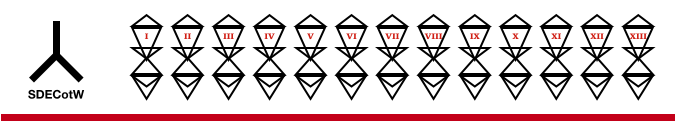
\includegraphics[width=\linewidth]{images/SCP-001-a-record.png}
	\caption*{下列收容措施由站点主管全体执行委员会(Site Directors' Executive Committee of the Whole)\\ 和O5议会全体一致通过}
\end{figure}

\bb{项目编号:}SCP-001

\bb{项目等级:}Thaumiel\ii{(主观评价)}

\bb{特殊收容措施:}依照站点主管全体执行委员会\footnote{\ii{SDECotW}。}于20██年5月3日一致作出的主观意见, SCP-001的数据库访问位置将被禁止编辑,仅可由O5议会成员所有的7份私人密钥修改。SDECotW的多数主观意见认为那之前被分类为SCP-001的物体不应再被给予SCP分类,并应当转存到Site-19的标准高价值收容锁柜中。

SDECotW全体一致认为任何情况下都不应在基金会数据库的SCP-001页面上做出客观宣言或陈述, 且只应有对过往基金会管理层意见的可证实真实记录。

根据O5议会在20██5月3日作出的多数意见,若Thaumiel实体,Mary Nakayama博士,或任何宣称是此人的实体与SCP基金会进行了接触,应该将其引导至O5议会以求进行谈判或合作。O5议会的多数意见认为当前不应该去尝试消灭Thaumiel实体、或是去尝试找到SCP-001数据库位置的薄弱点。

\bb{描述:}SDECotW和O5议会于20██5月3日全体一致认为,任何在特定SCP基金会数据库页面\bb{⦿\slash Procedures\slash 001\slash SCP-001.fmtl}上做出的事实性称述都会变为客观事实。该意见认为对这一页面做出的任何修改都会造成范围极其广阔、且很可能是无限范围的阿尔法室(“终极关注”)型现实修改情形;SDECotW和O5议会认为不应再对此效应进行更多测试,理由是这种测试有极高可能引发潜在的XK/CK/LK/VK/ZK/תK级情景。

SDECotW全体一致认为其它在基金会数据库\bb{⦿\slash Procedures\slash 001\slash}部分下的页面没有异常效应,使SCP-001效应被发现、并有可能创造出了Thaumiel实体的SCP-001数据过往版本应作为子页面储存在此目录下以供参考。

SDECotW全体一致认为必须对基金会数据库的所有空白位置进行检查,确认是否有更多的阿尔法室型现实修改异常;此外任何时候最多只能开放1000个经过彻底检查的数据库位供员工编辑新的特殊收容措施。

% =====

\newpage

\tred{▷⦿\slash Procedures\slash 001\slash Past\slash Feb_18,_20██_1.ftml}

\tred{▽⦿\slash Procedures\slash 001\slash Past\slash Feb_18,_20██_1.ftml}

\begin{scpbox}
\bb{基金会数据库修改记录:} \\
创建新SCP文件。在2███位置进行创建尝试,但项目的效应可能会让它自动移动到-001去。已让管理员解锁空白的001位置(为什么要空着?我想是图个方便)以防万一。 \\
- \ii{mnakayama},20██年2月18日11:34 AM
\end{scpbox}

\begin{figure}[H]
	\centering
	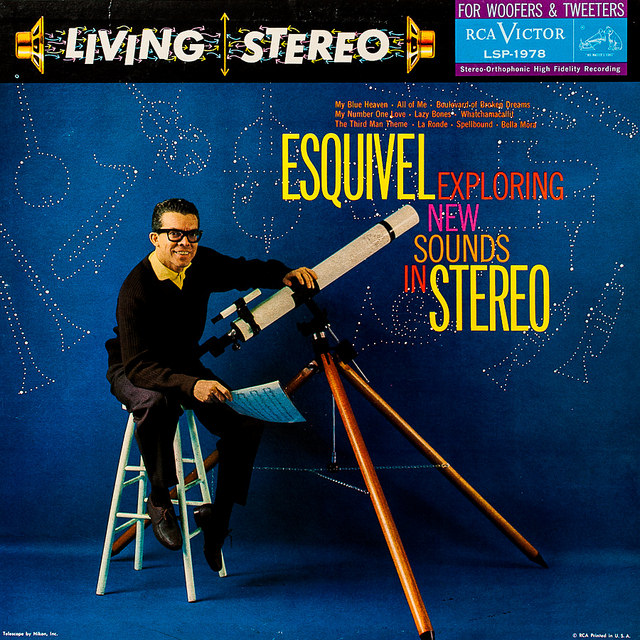
\includegraphics[width=0.5\linewidth]{images/SCP-001-a-record-2.jpg}
	\caption*{SCP-001的封面。唱片封面和无异常的再版封面相同。}
\end{figure}

\bb{项目编号:}SCP-001

\bb{项目等级:}Safe

\bb{特殊收容措施:}SCP-001将被收容于Site-91a的标准低价值收容锁柜中。对SCP-001效应的更多研究将由Site-91a首席数字命理学家Mary Nakayama博士负责。

描述:SCP-001是一张乙烯基唱片,内容为Esquivel发行于1958年的唱片《探索立体新声》(RCA)。该唱片会对将其纳入其中的数据化数字列表产生异常影响。若将该唱片列入数据保存的文本中,它将总是会被第一个列出,即便有意将其调至其他位置也是如此。\footnote{这一效应会扩散到一切形式的数据存储中。迄今受影响设备包括使用级电脑、移动电话、图表计算器。机械式存储设备,如书写或以物理形式表现地列表不会受到其异常效应影响。\label{footnote 2}}

SCP-001在1958年于发行前作为赠审阅副本送给了《公告牌》杂志。其效应一直未被发现,直至20██年十二月,《公告牌》杂志实习生M. S██████在将杂志总部过往审阅唱片的手工文件更新到数据库上时才发觉到其异常并向其上级进行了报告。\footnote{最初这起事件中可能的电子犯罪嫌疑引起了FBI注意。FBI电子犯罪部门内潜伏的UIU特工在发现该物品后将其给了基金会保管。\label{footnote 3}}

正在定位将SCP-001送到《公告牌》杂志的RCA员工。主流收容理论当前认为SCP-001是被用于试尝操控《公告牌》杂志的唱片排行榜,但由于当时该杂志还在使用人工打字,这一企图未能实现。

% =====

\newpage

\tred{▷⦿\slash Procedures\slash 001\slash Past\slash Feb_18,_20██_2.ftml}

\tred{▽⦿\slash Procedures\slash 001\slash Past\slash Feb_18,_20██_2.ftml}

\begin{scpbox}
\bb{基金会数据库修改记录:} \\
很好,真的自己移动过来了。奇怪。有趣。准备继续深入(可能有些隐藏的?)此外,修复了一个打字错误,感谢Dr Amoralles。 \\
- \ii{mnakayama},20██年2月18日11:41 AM
\end{scpbox}

\begin{figure}[H]
	\centering
	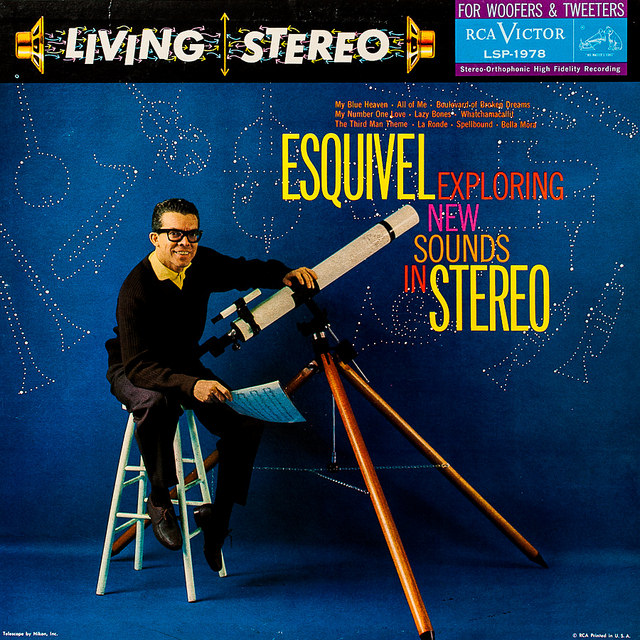
\includegraphics[width=0.5\linewidth]{images/SCP-001-a-record-2.jpg}
	\caption*{SCP-001的封面。唱片封面和无异常的再版封面相同。}
\end{figure}

\bb{项目编号:}SCP-001

\bb{项目等级:}Safe

\bb{特殊收容措施:}SCP-001将被收容于Site-91a的标准低价值收容锁柜中。对SCP-001效应的更多研究将由Site-91a首席数字命理学家Mary Nakayama博士负责。

\bb{描述:}SCP-001是一张乙烯基唱片,内容为Esquivel发行于1958年的唱片《探索立体新声》 (RCA)。该唱片会对将其纳入其中的数据化数字列表产生异常影响。若将该唱片列入数据保存的文本中,它将总是会被第一个列出,即便有意将其调至其他位置也是如此。

SCP-001在1958年于发行前作为审阅副本送给了《公告牌》杂志。其效应一直未被发现,直至20██年十二月,《公告牌》杂志实习生M. S██████在将杂志总部关于过往审阅唱片的手工打印文件更新到数据库上时才发觉到其异常并向其上级进行了报告。\footref{footnote 2}

正在定位将SCP-001送到《公告牌》杂志的RCA员工。主流收容理论当前认为SCP-001是被用于\red{\dd{试尝}}\green{尝试}操控《公告牌》杂志的唱片排行榜,但由于当时该杂志还在使用人工打字,这一企图未能实现。\footref{footnote 3}

% =====

\newpage

\tred{▷⦿\slash Procedures\slash 001\slash Past\slash Apr_1,_20██_1.ftml}

\tred{▽⦿\slash Procedures\slash 001\slash Past\slash Apr_1,_20██_1.ftml}

\begin{scpbox}
\bb{基金会数据库修改记录:} \\
对收容措施进行为期一天的重要修正 ;) \\
- \ii{mnakayama},20██4月1日9:41 AM
\end{scpbox}

\begin{figure}[H]
	\centering
	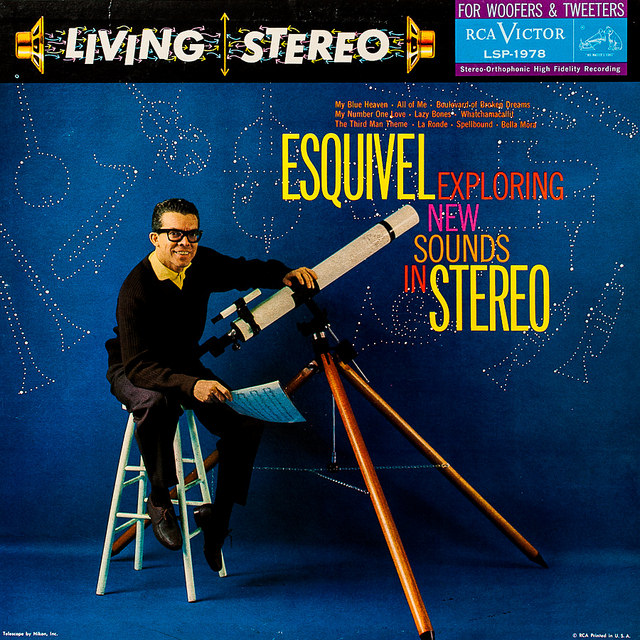
\includegraphics[width=0.5\linewidth]{images/SCP-001-a-record-2.jpg}
	\caption*{SCP-001的封面。唱片封面和无异常的再版封面相同。}
\end{figure}

\bb{项目编号:}SCP-001

\bb{项目等级:}Safe

\bb{特殊收容措施:}SCP-001将被收容于Site-91a的标准低价值收容锁柜中。对SCP-001效应的更多研究将由Site-91a首席数字命理学家Mary Nakayama博士负责。\green{所有Site-91a的2级研究员应当在20██年四月1日于Nakayama博士午餐时间向其支付5美元。}

\bb{描述:}SCP-001是一张乙烯基唱片,内容为Esquivel发行于1958年的唱片《探索立体新声》 (RCA)。该唱片会对将其纳入其中的数据化数字列表产生异常影响。若将该唱片列入数据保存的文本中,它将总是会被第一个列出,即便有意将其调至其他位置也是如此。

SCP-001在1958年于发行前作为审阅副本送给了《公告牌》杂志。其效应一直未被发现,直至20██年十二月,《公告牌》杂志实习生M. S██████在将杂志总部关于过往审阅唱片的手工打印文件更新到数据库上时才发觉到其异常并向其上级进行了报告。\footref{footnote 2}

正在定位将SCP-001送到《公告牌》杂志的RCA员工。主流收容理论当前认为SCP-001是被用于尝试操控《公告牌》杂志的唱片排行榜,但由于当时该杂志还在使用人工打字,这一企图未能实现。\footref{footnote 3}

% =====

\newpage

\tred{▷⦿\slash Procedures\slash 001\slash Past\slash Apr_1,_20██_2.ftml}

\tred{▽⦿\slash Procedures\slash 001\slash Past\slash Apr_1,_20██_2.ftml}

\begin{scpbox}
\bb{基金会数据库修改记录:} \\
这TM这TM这TM是·他·妈·的怎么回事。 \\
- \ii{mnakayama},20██年4月1日12:54 PM
\end{scpbox}

\begin{figure}[H]
	\centering
	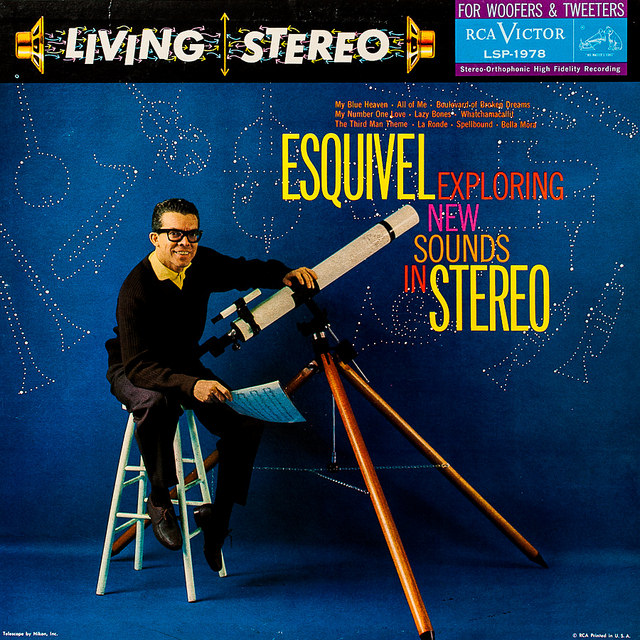
\includegraphics[width=0.5\linewidth]{images/SCP-001-a-record-2.jpg}
	\caption*{SCP-001的封面。唱片封面和无异常的再版封面相同。}
\end{figure}

\bb{项目编号:}SCP-001

\bb{项目等级:}Safe

\bb{特殊收容措施:}SCP-001将被收容于Site-91a的标准低价值收容锁柜中。对SCP-001效应的更多研究将由Site-91a首席数字命理学家Mary Nakayama博士负责。\red{\dd{所有Site-91a的2级研究员应当在20██年四月1日于Nakayama博士午餐时间向其支付5美元。}}

\bb{描述:}SCP-001是一张乙烯基唱片,内容为Esquivel发行于1958年的唱片《探索立体新声》 (RCA)。该唱片会对将其纳入其中的数据化数字列表产生异常影响。若将该唱片列入数据保存的文本中,它将总是会被第一个列出,即便有意将其调至其他位置也是如此。

SCP-001在1958年于发行前作为审阅副本送给了《公告牌》杂志。其效应一直未被发现,直至20██年十二月,《公告牌》杂志实习生M. S██████在将杂志总部关于过往审阅唱片的手工打印文件更新到数据库上时才发觉到其异常并向其上级进行了报告。\footref{footnote 2}

正在定位将SCP-001送到《公告牌》杂志的RCA员工。主流收容理论当前认为SCP-001是被用于尝试操控《公告牌》杂志的唱片排行榜,但由于当时该杂志还在使用人工打字,这一企图未能实现。\footref{footnote 3}

% =====

\newpage

\tred{▷⦿\slash Procedures\slash 001\slash Past\slash Apr_1,_20██_3.ftml}

\tred{▽⦿\slash Procedures\slash 001\slash Past\slash Apr_1,_20██_3.ftml}

\begin{scpbox}
\bb{基金会数据库修改记录:} \\
一些小测试。 \\
- \ii{mnakayama},20██4月1日9:09 PM。
\end{scpbox}

\begin{figure}[H]
	\centering
	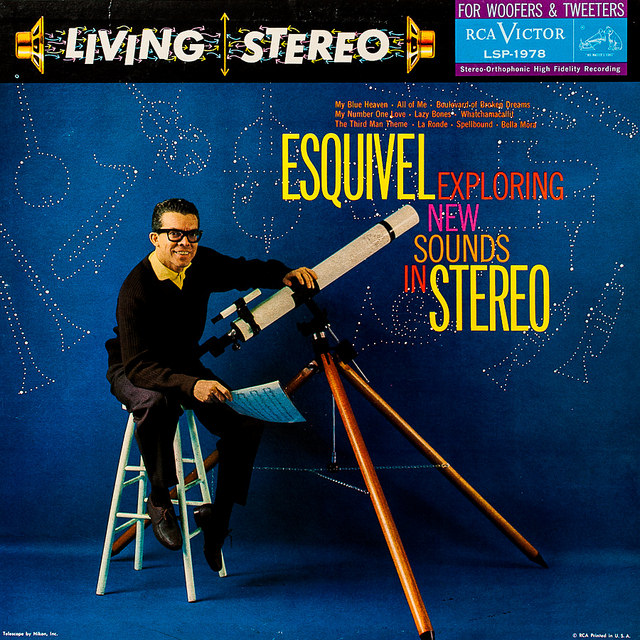
\includegraphics[width=0.5\linewidth]{images/SCP-001-a-record-2.jpg}
	\caption*{SCP-001的封面。唱片封面和无异常的再版封面相同。}
\end{figure}

\bb{项目编号:}SCP-001

\bb{项目等级:}Safe

\bb{特殊收容措施:}SCP-001将被收容于Site-91a的标准低价值收容锁柜中。对SCP-001效应的更多研究将由Site-91a首席数字命理学家Mary Nakayama博士负责。\green{Nakayama博士书桌上的名牌被染成绿色以便于识别。}

\bb{描述:}SCP-001是一张乙烯基唱片,内容为Esquivel发行于1958年的唱片《探索立体新声》 (RCA)。该唱片会对将其纳入其中的数据化数字列表产生异常影响。若将该唱片列入数据保存的文本中,它将总是会被第一个列出,即便有意将其调至其他位置也是如此。

SCP-001在1958年于发行前作为审阅副本送给了《公告牌》杂志。其效应一直未被发现,直至20██年十二月,《公告牌》杂志实习生M. S██████在将杂志总部关于过往审阅唱片的手工打印文件更新到数据库上时才发觉到其异常并向其上级进行了报告。\footref{footnote 2}

正在定位将SCP-001送到《公告牌》杂志的RCA员工。主流收容理论当前认为SCP-001是被用于尝试操控《公告牌》杂志的唱片排行榜,但由于当时该杂志还在使用人工打字,这一企图未能实现。\footref{footnote 3}

% =====

\newpage

\tred{▷⦿\slash Procedures\slash 001\slash Past\slash Apr_2,_20██_1.ftml}

\tred{▽⦿\slash Procedures\slash 001\slash Past\slash Apr_2,_20██_1.ftml}

\begin{scpbox}
\bb{基金会数据库修改记录:} \\
给自己请了个假。 \\
- \ii{mnakayama},20██4月1日9:09 PM。
\end{scpbox}

\begin{figure}[H]
	\centering
	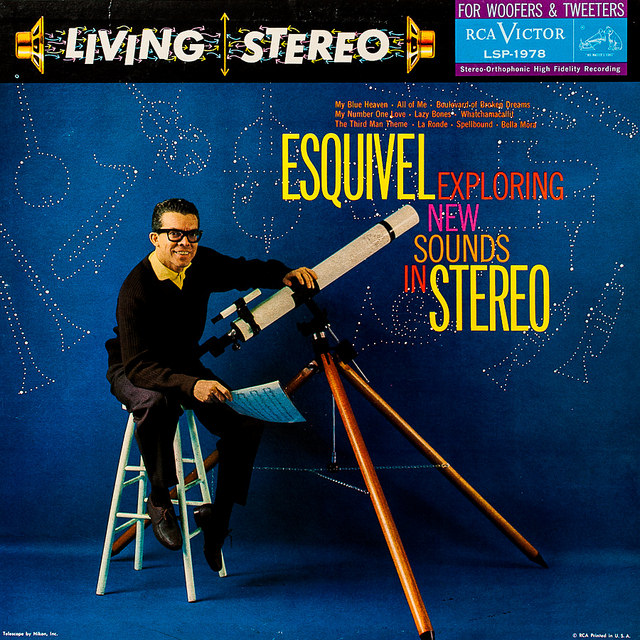
\includegraphics[width=0.5\linewidth]{images/SCP-001-a-record-2.jpg}
	\caption*{SCP-001的封面。唱片封面和无异常的再版封面相同。}
\end{figure}

\bb{项目编号:}SCP-001

\bb{项目等级:}Safe

\bb{特殊收容措施:}SCP-001将被收容于Site-91a的标准低价值收容锁柜中。对SCP-001效应的更多研究将由Site-91a首席数字命理学家Mary Nakayama博士负责。\red{\dd{Nakayama博士书桌上的名牌被染成绿色以便于识别。}}\green{通知所有人员Nakayama博士在20██4月9日前可能暂时不能工作,她已由站点主管Green批准在这期间休假。}

\bb{描述:}SCP-001是一张乙烯基唱片,内容为Esquivel发行于1958年的唱片《探索立体新声》 (RCA)。该唱片会对将其纳入其中的数据化数字列表产生异常影响。若将该唱片列入数据保存的文本中,它将总是会被第一个列出,即便有意将其调至其他位置也是如此。

SCP-001在1958年于发行前作为审阅副本送给了《公告牌》杂志。其效应一直未被发现,直至20██年十二月,《公告牌》杂志实习生M. S██████在将杂志总部关于过往审阅唱片的手工打印文件更新到数据库上时才发觉到其异常并向其上级进行了报告。\footref{footnote 2}

正在定位将SCP-001送到《公告牌》杂志的RCA员工。主流收容理论当前认为SCP-001是被用于尝试操控《公告牌》杂志的唱片排行榜,但由于当时该杂志还在使用人工打字,这一企图未能实现。\footref{footnote 3}

% =====

\newpage

\tred{▷⦿\slash Procedures\slash 001\slash Past\slash Apr_9,_20██_1.ftml}

\tred{▽⦿\slash Procedures\slash 001\slash Past\slash Apr_9,_20██_1.ftml}

\begin{scpbox}
\bb{基金会数据库修改记录:} \\
记录一下将要发生的头衔变动… \\
- \ii{mnakayama},20██4月1日9:09 PM。
\end{scpbox}

\begin{figure}[H]
	\centering
	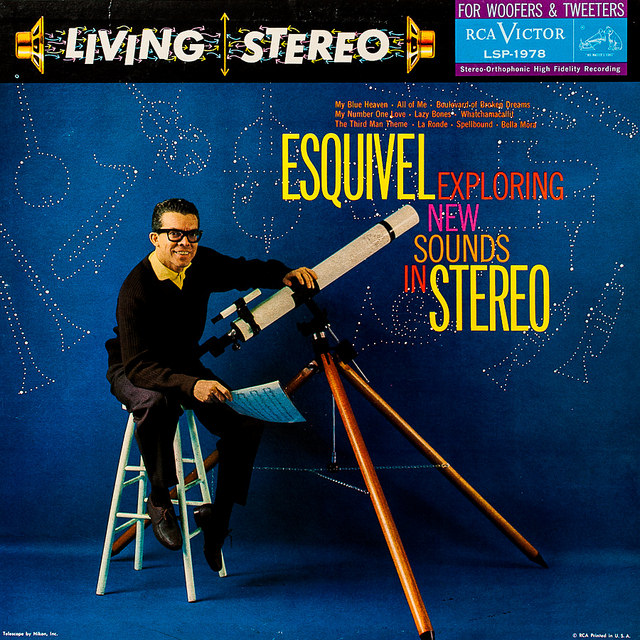
\includegraphics[width=0.5\linewidth]{images/SCP-001-a-record-2.jpg}
	\caption*{SCP-001的封面。唱片封面和无异常的再版封面相同。}
\end{figure}

\bb{项目编号:}SCP-001

\bb{项目等级:}Safe

\bb{特殊收容措施:}SCP-001将被收容于Site-91a的标准低价值收容锁柜中。对SCP-001效应的更多研究将由\red{\dd{Site-91a首席数字命理学家}}Mary Nakayama博士负责。\red{\dd{通知所有人员Nakayama博士在20██4月9日前可能暂时不能工作,她已由站点主管Green批准在这期间休假。}}\green{Nakayama博士,在4月9日以前的Site-91a首席数字命理学家,将在4月9日晚晋升为站点副主管协助Green博士工作。她将独立负责SCP-001项目。}

\bb{描述:}SCP-001是一张乙烯基唱片,内容为Esquivel发行于1958年的唱片《探索立体新声》 (RCA)。该唱片会对将其纳入其中的数据化数字列表产生异常影响。若将该唱片列入数据保存的文本中,它将总是会被第一个列出,即便有意将其调至其他位置也是如此。

SCP-001在1958年于发行前作为审阅副本送给了《公告牌》杂志。其效应一直未被发现,直至20██年十二月,《公告牌》杂志实习生M. S██████在将杂志总部关于过往审阅唱片的手工打印文件更新到数据库上时才发觉到其异常并向其上级进行了报告。\footref{footnote 2}

正在定位将SCP-001送到《公告牌》杂志的RCA员工。主流收容理论当前认为SCP-001是被用于尝试操控《公告牌》杂志的唱片排行榜,但由于当时该杂志还在使用人工打字,这一企图未能实现。\footref{footnote 3}

% =====

\newpage

\tred{▷⦿\slash Procedures\slash 001\slash Past\slash May_3,_20██_1.ftml}

\tred{▽⦿\slash Procedures\slash 001\slash Past\slash May_3,_20██_1.ftml}

\begin{scpbox}
\bb{基金会数据库修改记录:} \\
很好。一切如我所想。我已经准备了好几个星期;现在是时候了。我已经把这个页面对所有人锁定,除了我自己和O5们。我想我是在做一件正确的事。这是我的真实想法。为我祈祷吧。 \\
- \ii{mnakayama},20██5月3日4:11 AM。
\end{scpbox}

\bb{项目编号:}SCP-001

\red{\bd{项目等级:}\dd{Safe}}

\red{\bd{特殊收容措施:}\dd{SCP-001将被收容于Site-91a的标准低价值收容锁柜中。对SCP-001效应的更多研究将由Mary Nakayama博士负责。Nakayama博士,在4月9日以前的Site-91a首席数字命理学家,将在4月9日晚晋升为站点副主管协助Green博士工作。她将独立负责SCP-001项目。}}

\red{\bd{描述:}\dd{SCP-001是一张乙烯基唱片,内容为Esquivel发行于1958年的唱片《探索立体新声》 (RCA)。该唱片会对将其纳入其中的数据化数字列表产生异常影响。若将该唱片列入数据保存的文本中,它将总是会被第一个列出,即便有意将其调至其他位置也是如此。\footref{footnote 2}}}

\red{\dd{SCP-001在1958年于发行前作为赠审阅副本送给了《公告牌》杂志。其效应一直未被发现,直至20██年十二月,《公告牌》杂志实习生M. S██████在将杂志总部过往审阅唱片的手工文件更新到数据库上时才发觉到其异常并向其上级进行了报告。\footref{footnote 3}}}

\red{\dd{正在定位将SCP-001送到《公告牌》杂志的RCA员工。主流收容理论当前认为SCP-001是被用于尝试操控《公告牌》杂志的唱片排行榜,但由于当时该杂志还在使用人工打字,这一企图未能实现。}}

\green{Mary Nakayama,在本文档保存后立刻获得全知与全能,扬升到并成为神。她将超越一切时间,对这宇宙和现实具有完全的统治权。一切事物,一切事物之下的事物以及一切事物之上的事物,都将服从于她的命令。她将得到对在保持和利用这些能力的同时能维持自身意识清醒持续的一切必要心灵性质。}

\green{O5议会成员收到一份说明SCP-001性质的笔记。}

\green{她的家人将收到一份笔记,其中会表明她对他们的爱。}

\begin{scpbox}
Mary Nakayama在5月3日晚六点前从Site 91的宿舍中失踪。至今仍未被找到。
\end{scpbox}

% =====

\newpage

\tred{▷20██年5月3日早存入Mary Nakayama电脑内的文件}

\tred{▽20██年5月3日早存入Mary Nakayama电脑内的文件}

\cl{
致O5议会,

在我十五岁时,我曾吃下过可以杀死我四次的药,给自己灌了一整瓶廉价伏特加,这是那个利用了我又把我抛下、任我心碎孤单的男人唯一留下的东西。

我坐在浴盆里任由热水炽烫我的身体。我闭上了眼睛。

当我睁开眼,我身上的水已经干了。一切安好。我躺在床上。在门边,一个闪烁的身影,发着光芒。盘旋着。它用一个只在我心中回响的声音向我开口说话。它说我有更伟大的事要做。

我再也没有看见过它。但我仍在继续前行。我相信那是上帝降临拯救了我。而,加入基金会后,我还怎么可能不相信呢?还有别的理由能解释为何我们仍存在于此、仍奇迹般地、绝望地、尖叫地活着的事实么?还有别的理由能解释我们世界的根基,我们的一切,竟能经受住这些我们每日面对的异物么?我们被保护着。我每夜向它祈祷指引。我再也未能听到那声音。

我曾触到上帝,那是改变我一生命运的时刻。

但当我在一篇文档上按下“保存”就把自己桌上的名牌变色时,我意识到了什么。万事万物的根基已向我开启。我本可抛下这力量,向你们报告,或者隐瞒它,但…

若这就是拯救我们的关键呢?如果它就是拯救我们所有人的关键,如果就是它在每一天从那些撕碎我们世界脆弱稳定的深渊噩梦手中保护着我们呢? 如果在一个文本里按下“保存”真的就是上帝的诞生呢?

若它不是,那就让我来尝试。若它就是,那就让我来监控它。我会试着将一切纠正。这可能会花些时间。

祝我好运。

- \ii{MN}
}



\chapter[SCP-001 破碎之神]{
	SCP-001 TwistedGears/Kaktus -The Broken God \\
	SCP-001 破碎之神
}

\label{chap:SCP-001.the.broken.god}

\begin{figure}[H]
	\centering
	\fbox{
\includegraphics[width=\linewidth]{images/SCP-001-the-broken-god.png}}
\end{figure}

\cl{

\GG{\bb{根据O5议会指令}}

\Gg{\bb{下列文档描述了Maksur级异常实体}}

信息受5级机密保护。Maksur级信息的泄露被严厉禁止,且将对SCP基金会及其利益造成严重威胁。访问文件的人员须提供5级安保许可,并接受了对AZ109模因危害的预防接种。未能遵照者将在访问文件时立即遭致“携带者奥米茄”模因处决。

\tred{[提交5级安保许可]}

\tred{[安保认知危害启动]}

}

\begin{figure}[H]
	\centering
	\{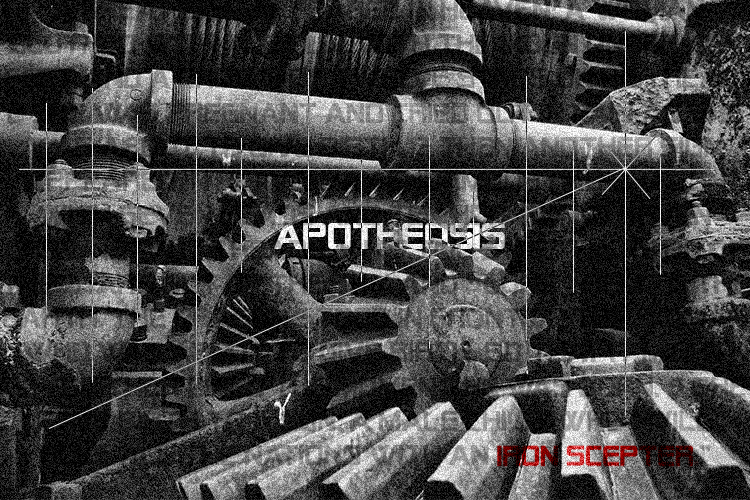
\includegraphics[width=\linewidth]{images/SCP-001-the-broken-god-2.jpg}
\end{figure}

\cl{

\bb{侦测到生命迹象}

\bb{模因接种查明}

\bb{欢迎,监督者}

}

\hr

\begin{figure}[H]
	\centering
	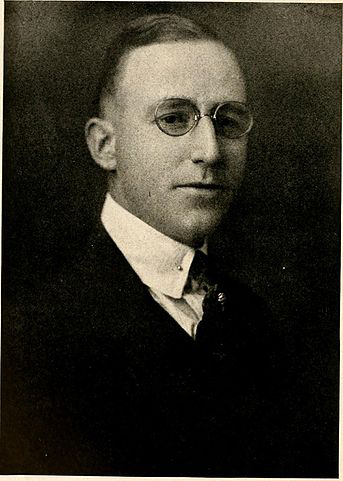
\includegraphics[width=0.5\linewidth]{images/SCP-001-the-broken-god-3.jpg}
	\caption*{Robert Bumaro,破碎之神教会现任领导者。日期未知。}
\end{figure}

\bb{项目编号:}SCP-001

\bb{项目等级:}Maksur\footnote{Maksur分级在1981年由基金会收容委员会联合监督者议会、站点主管议会、基金会伦理委员会联合编入规范。在Maksur级被规范化前,SCP-001曾被编为“Neutralized”,Maksur分级被制定用于替代此不当分级(参加机密委员会记录CA-10931“Neutralized分级在分标准应用中的关联性” CA-10945, “提案:Maksur级”)}

\bb{特殊收容措施:}相关异常项目与SCP-001间存在关联性的信息将在各自文件中被删改。这些项目与破碎之神教会的关联可以保留,但其来源将被删改或模糊处理。

SCP-001的非活跃部件将被留在原地,在其所处区域内禁止任何行船或潜水。平民对SCP-001的察觉将被压制,并使用记忆删除以维持保密。破碎之神教会相关人员若做出寻找SCP-001非活跃部分的举动,将被基金会拘留并审问。关于SCP-001的一切信息,无论是实体还是数据,都将被没收收容。

SCP-001的非活跃部件被预期将保持在无活动状态;然而,若SCP-001出现自发复苏,所有在Site-27, Site-44, Site-90及Site-101附近的活动中机动特遣队单位将被派去采取收容措施。若该事件(当前编为001-登神事件)在现代世界发生,确信当前采取的信息压制措施不足以应对之。001-登神事件极有可能导致一次SK级“破碎面纱”情景\footnote{SK级情景将自动使基金会全部敏感信息备份到自我收容的“深井”站点(当前117、118和119)内最高级安保服务器中。所有非必要人员将接受人工记忆删除治疗,所有主要地方站点将进入全面封锁。当前模型下,该状态尚不确定。},之后将可能是XK级“世界末日”情景。

现存仍活跃的SCP-001部件任何情形下不得进入非活跃部件周围20km内。

\bb{描述:}SCP-001是一系列异常物体之集合,此前曾是破碎之神教会在1942年晚期于墨西哥拉巴斯组装的单一巨型机械实体。这些物体包括\hyperref[chap:SCP-217]{SCP-217},\hyperref[chap:SCP-1139]{SCP-1139},\hyperref[chap:SCP-882]{SCP-882}和\hyperref[chap:SCP-629]{SCP-629}的部分内部零件\footnote{在与破碎教会线人合作收容\hyperref[chap:SCP-629]{SCP-629}后才发现此事。未知这些部件是如何被 Wondertainment博士在基金会及破碎之神教会内部线人不知情的情况下收集到,也不知\hyperref[chap:SCP-629]{SCP-629}自身是否知晓自己与教会的联系。}。完整列表参见\red{这里}。

教会成员将这些异常物体组装在一起,意图以此修复他们信奉的神明。在启动后,据报告SCP-001开始将金属物体整合到自身之中,并开始积极寻找其他异常物体。SCP-001,以及因其被组装而引发的“001-登神”事件,造成了西墨西哥环境发生剧变,并引起了有记载以来最大范围的一次记忆删除施用。在事件后,仍然活跃的SCP-001部件被基金会带回站点收容,非活跃部分则被留在了加利福利亚湾底部,约在23.807269,-108.418369处。

\bb{附录001.01:}描述SCP-001的已收集信息

\begin{scpbox}

\ii{Jorge Castillo神父的陈述抄录,1945年8月}

Fernand是第一个…我觉得,是他们找到心脏后第一个联系我的。他们描述它的方式,还有眼中的狂热,令我迷惑,接着我知道了。我知道他们已经完成了。

在我姐姐的坚信礼后我在周末与Anthony及Salvador见了面…当他们向我展示时我被惊住了。它简直就是一堆齿轮、活塞、发条零件和上油金属部件的混合体,每个部件忠实地相互搅动且没有动力来源。在内部我看到了心脏,一如他们所描述。

它对我说话了。不像你与我这种对话,而是…用图像和感觉。还有痛苦。它处在如此的痛苦中。就像那曾经赋予它生命的火花也让它察觉了自己为何物,又或者不是何物,它只愿再次完整。

愿望这个词也许太过了。不是愿望,更多的是冲动。那造物中的什么东西驱使它向着不假思索、不会动摇的结局前进。他们呈现给我的这个造物和我曾发现并祝福的一切器物都不同。这一个不一样,它有什么地方不对,直到他们完成我才明白过来…

我请求Salvador把它带回\hyperref[chap:SCP-2217]{海岸}拆除,这样是不对的,但他们不可能听进去。在我离开前它已经开始动了。从一头到另一头开始振动,开始走动了。它蹒跚着走过一个扳手,那扳手就变成了它的一部分。他们对我说,“我们的神不破新生了!”

我再没见过他们。

\end{scpbox}

\begin{scpbox}

\ii{1946年对Francis Bollinger的采访}

它不用语词,或者任何语言。它发出金属的声音但同时…当我们靠近图像和概念就涌入了我们心中。你可曾感觉到,当你有了一个思绪或念头-它完全就在那,在你的思维中完整地诞生-但你还是必须去思考与之对应的语言,虽然你在完成句子前就知道了观点?那就像是这样,但却是来自另一个心灵。真正的神之言。

\end{scpbox}

\begin{scpbox}

\ii{2007年对特异事故调查单位特工Trixie Silva的采访}

那里有几个狼-等等,你们知道那是啥对吧?他们就像…就像猎人,为地平线倡议工作。他们在圣玛格丽塔的教堂附近遇到了我们,要我们交出从破碎之神教会那里招来的东西,就像以前我们移交过的亚伯拉罕类物品。

我们讨论起应不应该交出去-我们和地平线的立场有些动摇,更多是最近的事情。我们和当地的破碎教会关系不错,但这些狼…好吧要更有攻击性。我们看着手里的东西,这时候那个女人走了过来。我不知道她从哪里来的。她穿的就像嬉皮士;很瘦,头发上绕着铁链,但她看起来和整个时代完全不合。她眼睛里的凝视,她诡异的笑容,就像她几乎不在那里。

她看着我们拿的东西说她就要这个,噢。我其实并不清楚那到底是什么。一个金属盒子,呼呼又咔嗒地响着,我捡起来的时候边缘还放出了点光。比我原以为的还要亮些。我问这对她为什么那么重要,她说向我展示要比说简单。

她闭上眼低下头。之后她没有动也没有说,我也只好把眼睛闭上了。她把额头靠向我的,但有点分开。我们站了大概一秒,foi muito estranho,接着她突然把下巴往下挪了挪,让我也被向下一拉。

世界在我脚下掉落,我坠了下去。有什么东西在我的思绪里咔哒作响,是一幅双齿轮的图像,先是紧密结合,现在分离开来。我感到脊柱的骨突随我弯腰而伸展,只一步我便同行星这多维的螺丝钉合在一起。它环绕太阳熔炉旋转,被重力锁链所牵引,我们用弹簧无限拉伸的力量,一并飞过这多油的宇宙…

…抱-抱歉。这是一次体验。不,不是宗教体验。但…对。她让我把盒子捡起来,我感觉它好像重了点。我分不清到底是真变重了,还是我感觉它更加…重要了。我把盒子交给她,完全没听到狼或者队友或者上级的声音。

\end{scpbox}

\bb{附录001.02:}1945年6月对被开除的前破碎之神教会牧师Dolorous Randall神父的采访。

\begin{figure}[H]
	\centering
	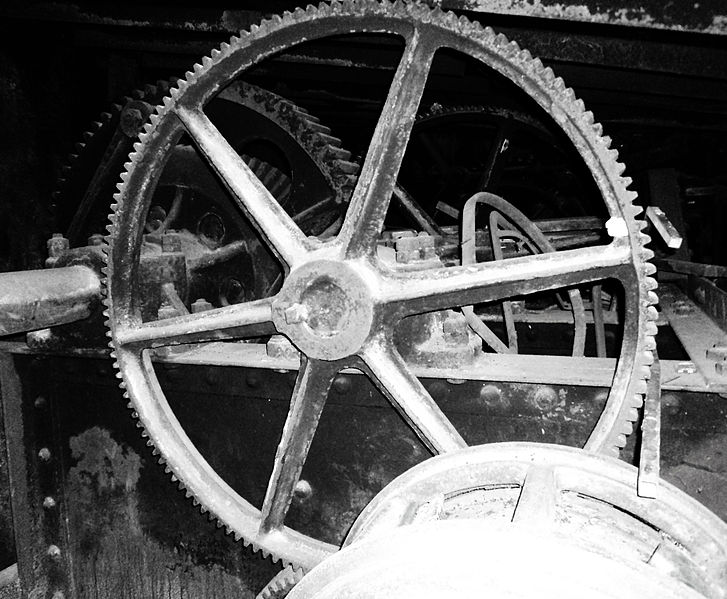
\includegraphics[width=0.5\linewidth]{images/SCP-001-the-broken-god-4.jpg}
	\caption*{在破碎之神教会仓库拍摄的照片。被确信为SCP-001的早期化身。}
\end{figure}


\begin{scpbox}

[多余部分略去]

\bb{Williams:}好了。你早先提到了心脏。他们找到它的时候你可在场?

\bb{Randall:}不,完全没有。那时我在国外,在巴拿马处理一个新任务。我只在事后听说了Ezekiel。

\bb{Williams:}Ezekiel是谁?

\bb{Randall:}Bumaro的一个特工。他身边总有这么一群人,与神协调能感受它的存在,与它对话。Ezekiel曾经发现了个挺重要的器物,Bumaro随后让他加入了。这些特工也是第一批接受改造实验的。如你所想,死了很多。

\bb{Williams:}但Ezekiel没有?

\bb{Randall:}没有。他和Bumaro很亲近,我不知道他会不会拿Ezekiel的健康冒险。这不重要,Ezekiel不需要改造也能与神对话。他就是…能够。

\bb{Williams:}所以Ezekiel对心脏做了什么?

\bb{Randall:}你听Avery说过他们有一大堆器物储备,对吧?这些特工碰过的任何东西,只要他们在其中感觉到了什么,就会被送到拉巴斯和其他的放在一起。大部分都是无价值的,但迟早他们会发现正品。精炼者,那一个-无论你们怎么称呼,一个特工在尼泊尔附近发现了它。他们有了筋腱和韧带等等一切,但都是只是部件。它们都可以自己活动,但不能在一起做什么。

\bb{Williams:}你什么意思?

\bb{Randall:}经典说神会在碎片被带到心脏面前时自行重整。只需要把手臂交给心脏,神就能得到一根手臂。但他们就是找不到心脏。他们(停顿)几个特工曾宣称找到了,但仍是和其他部分一样的无用机械碎片。

\bb{Williams:}Ezekiel在这之中是什么角色?

\bb{Randall:}Ezekiel 是那个告诉Bumaro,如果找不到心脏也许可以自己做一个的人。很快就知道这计划不会持续到夏季过完。我在Ezekiel走后被派去为他们找补给,他们的供应快要耗尽了。

\bb{Williams:}我们的记录显示心脏是被发现的。这不是真的?

\bb{Randall:}当然不是真的。你肯定不能给教众宣道说神把他的部件赐予你然后转身又说其实大部分基础部件都是你自己凭空拼造的。但至少比没有好。他们创造心脏并让它活过来的细节从没向我透露,但我能从蛛丝马迹里得到结论。那年有过一次旱灾,脊髓灰质炎危机又史无前例严重。数千人死亡,都是自然原因。一次可怕的事件,因为注意力都在战争而从未被准确记录过。神啊,但谁说得清呢。

\bb{Williams:}你觉得这两者有联系?

\bb{Randall:}我觉得时机太巧了。而且既然我知道那东西最后变成了什么,我想答案很清楚了。那不是神之心脏,特工。那是完全不同的什么东西。

[多余部分略去]

\end{scpbox}

\bb{附录001.03:}回收到的视频抄录,1942年11月

\begin{scpbox}

\ii{视频回收紫当地纪录电影团体。}

镜头从被破坏的房屋开始,车库周围满是残骸。金属碎片和橡胶条痕迹从车道延伸到沥青路,之后继续到街道上。各种车辆残片散落在街道和沿街上。这些痕迹引向正在将一辆卡车吞入自身底盘的SCP-001。

SCP-001继续向最近的房屋前进,开始吞食排水沟。区域居民逃离现场,多人被SCP-001丢下的玻璃渣和扭曲金属击伤。SCP-001身体的多个部分发出光芒,照在多个跪伏的人影上。SCP-001继续沿街道搜寻更多材料源,其底盘上一个部分变形从主体上落下。

伸出的部分继续变形,形成一个类似人类脊柱及肋骨架的垂直荚体。荚体多处破损,肋骨状突起从中伸出,其余荚体变形为一高约3米的人形实体。光从其头部发出,投在附近的平民上。

金属人形抓起似乎已死亡的平民,将其放入肋骨间的小空间内。肋骨随人形实体靠近第二名试图爬走的女性平民而摆动。实体将挣扎的平民举起放入胸腔内。之后人形实体转身背对摄像头向第三人前进,似乎是女子断手的物体掉落在地。

人形实体的后背上随其收集人体而长出一缓慢增大的赘生物,人形实体的身体大小也随之变小。在吞噬到第六人后赘生物已经大过了人形,使其无法再两足行走。其肢体已收回体内,肋骨伸出使其爬上了附近一栋房屋的屋顶。

它在原地停留了20分钟。球状物外层破裂后从内部裂开,露出三个人形实体。它们看起来是SCP-217感染者,表现出六名被吞食平民的身体特征。其中一名女性头皮上连着锁链,摇晃着另一个似乎已死亡的个体。第三人是一长着发条胳膊的男性,检查自己后跳下了楼顶,腹部着地。它似乎并未因此受伤,令其更为紧张。之后它开始追赶在街道远处吞噬其他汽车的SCP-001。

女性人形注意到了摄像者,开始挥手,但很快停止。它看向SCP-001后跳入后院,离开镜头中。

\end{scpbox}

\bb{附录001.04:}与Robert Bumaro谈话的电话录音。 \\
\ii{备注:下面破碎之神教会一名特工(姓名未知)和Robert Bumaro的电话交谈录音。该次通话记录在1942年12月,由基金会人员在1966年对一处教会据点进行搜查时获得。}

[播放音频]\footnote{
编者\QIS:在\href{http://scp-wiki-cn.wikidot.com/twistedgears-kaktus-proposal}{文章的Wiki页面}上此处是一个Flash控件,点击按钮可播放音频。由于大多数PDF不支持交互操作,所以没有导入。可以点击\href{http://scp-wiki.wdfiles.com/local--files/twistedgears-kaktus-proposal/bumaro.mp3}{这里}访问该音频。
}

\begin{scpbox}

[通话开始]

\bb{Bumaro:}你好?

\bb{Agent:}祝福您圣父。

\bb{Bumaro:}Dmitri?

\bb{Agent:}不。

\bb{Bumaro:}哦,当然。祝福你,孩子。小主如何了?

\bb{Agent:}日渐强壮。我们已将他从办公室后面挪入了附近的仓库。

\bb{Bumaro:}喂过他了吗?

\bb{Agent:}如您要求。

\bb{Bumaro:}很好。你何时去Puerto Peñasco?

\bb{Agent:}本周内。我们就等下列车。

\bb{Bumaro:}可能还得快点。几周前拉巴斯被突袭了一次。我们有三个人没有被找到。基金会活动越发活跃在-(暂时挂断)

\bb{Agent:}圣父?

\bb{Bumaro:}(对背景的某人)明天,明天。

\bb{Agent:}圣父?

\bb{Bumaro:}是的。我们曾期望他们北上,但他们却去了西边。小挫折。

\bb{Agent:}那安全屋呢?有将近一百件其他器物在那里,而且—

\bb{Bumaro:}(打断)小挫折。他们不知道在哪,就算他们知道了,这也不是他们的优先项目。他们的眼线,还有他们在世界上的其他眼线,都注视着欧洲。只要他们的目光落在那里,就不会发觉我们的完成直到已经无力阻挡他。

\bb{Agent:}这,嗯,还有其他事想问您,圣父。

\bb{Bumaro:}是的?

\bb{Agent:}我们的神,呃…太饿了。我们似乎无法满足他,我们得到的供给不—

\bb{Bumaro:}(再次打断)问题是什么?

\bb{Agent:}圣父,我们的…主在吃他自己的住所。我们无法劝服他停下,不能和他讲理,它-

\bb{Bumaro:}胡说。虔诚的心可以与神直接对话。当他靠近时你不能听到他的话吗?没有感觉机械在你心中运转?或者连在眼前呼吸鲜活的神也不能让你坚信?

\bb{Agent:}不!圣父,不是这样,是-

\bb{Bumaro:}我不会再听了。这么多年,我们祈祷、期盼神在我们面前不破新生。现在,他已展现了自己。我们知道神会对虔诚之心开口。如果你要告诉我,你们中连虔诚到能与神沟通的人都没有,现在就告诉我把你们换掉。

\bb{Agent:}我们的信念依然坚定,圣父。请您原谅我的无礼。我只是迷途了。

\bb{Bumaro:}那就自己反省。我担心你的信念。去找个弟兄,找个信念比你坚定的,让他去和主对话,告诉他保密的必要。我们的主将会理解,毫无疑问。不破之神是一位理智的神。

\bb{Agent:}是的,祝福您圣父。

\bb{Bumaro:}祝福你,孩子。

[通话结束]

\end{scpbox}

\bb{附录001.05:}增补报告,1943年12月 \\
\ii{下面是对基金会Site-74指挥官Mark Peterson的采访。主管在001-登神事件前驻扎于墨西哥城,事件期间与拉巴斯的基金会人员一同在站。}

\begin{figure}[H]
	\centering
	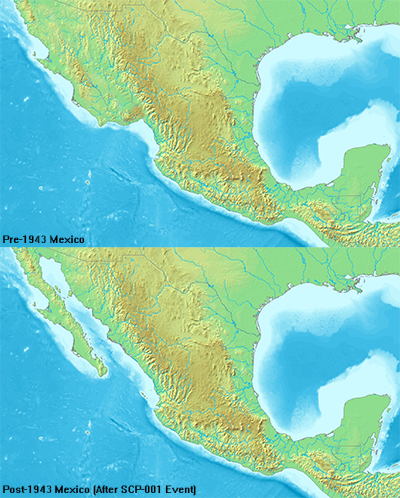
\includegraphics[width=0.5\linewidth]{images/SCP-001-the-broken-god-5.png}
	\caption*{001-登神事件前后的墨西哥}
\end{figure}

\begin{scpbox}

\bb{Director Cornwell:}从头再来一遍,我们在记录。

\bb{Commander Peterson:}好。关于教会活动的第一次报告是在41年,但那时候还都是非常小的事。我们刚刚完成了北部边境附近的外勤行动,正要准备把资产搬去亚特兰大准备法国的任务。我们已经接到命令,去收回一些他们不愿意被德国佬抢去的敏感物品。他们还准备派出我们整个部门去完成此事。领导不确定罗斯福会不会打电话为我们留下充足时间协同美军,所以我们必须得单独前进。

\bb{Director Cornwell:}你为何留在拉巴斯?

\bb{Commander Peterson:}我完全是偶然在那。我们的一辆列车取道往拉巴斯的陆路,也许是要顺路去取回一些军备。结果那趟列车本来是要北上的。所以突然之间大部分格兰德河以南的领导层就跑到了拉巴斯来,回想起来从整体效果看这倒可能帮了我们大忙。

\bb{Director Cornwell:}你何时首次听闻001-登神实体?

\bb{Commander Peterson:}(笑)耶稣啊。现在他们这么叫那东西了?那个机器,我猜, 我们第一次听说,是有本地活动频繁的风声,在…我猜大概得是一年多以前。我们在42年10月到了拉巴斯,所以…对,听起来没错。我们搞的第一个确凿证据是在一辆… 难民车?虽然这么叫着很傻但我想是准确的。他们在十月末来到拉巴斯,说整个镇子都被盖住了。他们没有真正的解释什么,就是一直说“la máquina, la máquina”, 你知道的,“机器”。顺便这就是我们那么叫它的原因。我们还完全不清楚那应该是个什么。

\bb{Director Cornwell:}那你和该实体的第一次接触呢?

\bb{Commander Peterson:}好吧,铁路停止运营了,如果你是这意思的话。我们听当地警方说北边出了事故,列车不会再往边境开了。这对我们来说可是大问题,我们可不能坐着几辆车向东走到山脚小镇为止。它们大多都和单独的铁道线完全挂钩,我们本可以就那么走。但是大东西,那些列车要去拉巴斯拉的东西,不能动。所以我们得等着。之后DeMarco想出个注意,派支小队沿铁路看看堵塞在哪,我们能不能清理掉它。他自己领队。

\bb{Director Cornwell:}特工DeMarco怎样了?

\bb{Commander Peterson:}你他妈知道他出什么事了Bill。

\bb{Director Cornwell:}为记录。

\bb{Commander Peterson:}好吧。我们三天没有收到回信,于是准备把剩下的领导层送去东边免得再等了。但五天后DeMarco的一个部下回到了营地。他精神混乱,说着“吞世怪物”,还有其他所有人都被盖掉了的话。他们是被盖掉了不是吗?我知道那时候它还不是最后那么大,但也不是可以应付的东西。DeMarco…

\bb{Director Cornwell:}你没事吗?

\bb{Commander Peterson:}没事。他试过想杀掉它。但接着他也许明白了我们之后才弄明白的事;我们不可能收容这东西。世界上没有哪个洞大到能装下它,或者有什么盒子是它吃不掉的。但这对他没意义了,其他跟着他去的人都是。那机器不关心这些。

\bb{Director Cornwell:}你什么时候第一次看到了它?

\bb{Commander Peterson:}十二月。在我们蹲守期间,我加入探索队溜过去看个究竟。它已经…我是说,你看过它对边境做了什么。我从来没看过大成这样还能动的东西。就感觉是一座活动部件堆成的山染黑了天空,好像它是在烧那些被它铲进胸口的东西一样。然后它又小了!它… 我不知道。我们都接受有XK-事件准备训练,但这个超出或者说在我们受过的任何训练之外。它就是无敌的。我们知道我们是去送死,那东西要杀了我们,只是个时间问题。

\end{scpbox}

\bb{附录001.06: }收集到的基金会通信 \\
\ii{备注:下面是拉巴斯驻扎基金会人员的书面通信摘录,在001-登神事件后回收于临时站点。姓名已隐去。}

\begin{scpbox}

亲爱的███████,

我甚至不知道这封信能不能送到。列车全停了,但指挥官说还能把信送出去。我希望确实如此,希望你能读到。

这里的天空已经暗了好几周了。每天北边都有烟飘来,呼吸都很困难。这里还是没有室内水管,除了我们公司的另一些人外都不说英语。

我们还是不知道我们在这里干什么。我一直听说要修铁路,但为什么不去北边?不是北边的铁路坏了吗?

\end{scpbox}

\begin{scpbox}

今天有个男人来到镇上,基本上半张脸都被煮过一样。他就像个死人,对谁都不回应。他走到镇中间就倒地了。在医务室醒来后,他变得很激动。说什么山一样大的机器还能和你说话。说那里有人从各自家里跑出来,把自己扔到它身上。说他们被碾碎,像是在草坪修剪机下面跳一样。之后他就死了,没人知道怎么回事。

\end{scpbox}

\begin{scpbox}

山脉在我们面前被撞碎。我们看到一个身影从烟中立起,缓慢笨重但势头恐怖。它不是像野兽一样爬行或是人一样走动,而是靠着几百万齿轮转动推进,就如钢铁的眼镜蛇。它的身体向前伸出,进入烟中,高过我们所能触及。在它的胸口里我看见有火在跳动,就像地狱的熔炉。它来到我们北边的山前,却没有停下或是绕路,而是就这么穿了过来,把山峰全部吞噬。它身处一条长胳膊,将整个村庄抓起塞进口中。我看到人们随家园被抹去一并走向死亡,和其他人一起投身地狱中。接着它叫了,不是齿轮的嘎吱或机械的轰响,而是在我们的心里。我能在心里听到它。它在嚎叫。

\end{scpbox}

\begin{scpbox}

\bb{指令:}中央指挥部,Site-001

\bb{敬礼:}█████████████

临时站点损失。拉巴斯成为废墟。机械实体被收容。大规模地理改变。XK已避免。申请记忆删除支持。

\end{scpbox}

\bb{附录001.07:}采访GOC中尉“归来者” \\
\ii{备注:下面是对全球超自然联盟中尉、代号“归来者”的事后采访摘录。采访记录及全部抄录由基金会特工在1992年的协商情报交换中获得。迄今“归来者”的身份仍然未知。}

\begin{figure}[H]
	\centering
	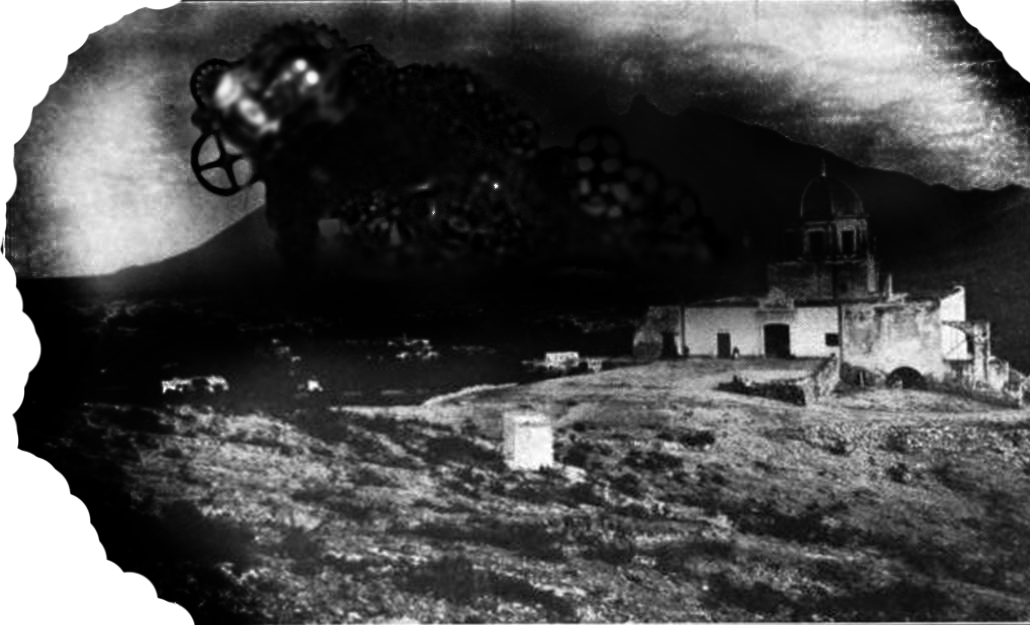
\includegraphics[width=0.5\linewidth]{images/SCP-001-the-broken-god-6.png}
	\caption*{SCP-001,照片拍摄于事件后且严重受损,拍摄者未知}
\end{figure}

\begin{scpbox}

基金会特工里流传着一些故事,就是那种白头老兵在长夜值岗或者在小房间里讲给新兵蛋子的故事。我不知道是谁开的头,但我知道他们现在还在讲。已经半个世纪过去了,他们确实还是对的,你就是可以给他们如此信任。他们说,“你知道么,GOC杀了神。”

但新兵就会说,“不,这不是真的。神被收容在Site-管他是哪呢。反正GOC没有杀过神。”接着他们就会讨论起被他们锁在某处的绿型,那个说自己是基督教上帝的家伙。但这时老兵只会摇摇头,笑而不语。因为他们都知道。

他们都知道在1943年,在末日之中,基金会只能眼看着GOC拯救世界,什么都做不了。

隐喻枪是在希腊海岸边的一座岛上被发现。我甚至不记得它长什么样了,我记得的只剩下记忆删除留给我的那一点模糊回忆。但我本能地觉得它不是你以为的那么重。

为什么记忆删除?那时候我跟着地区部署的分遣队,显然有一块碎片让它造成了心智影响。我模糊地觉得有什么不对,所以我听了他们的话。我不记得它长什么样,我也想不起来它是如何毁掉那么多大陆的。该死,我只记得它何时发生,知道这事的唯一原因还是前后地图的变化。但我还是能感觉到,我的本能说,事情本不该如此。我们站在一个愤怒的复仇神面前,而它做的全部事就是祈求我们杀掉它。

我们全都是如此乐于履职。

\end{scpbox}

\bb{附录001.08:}记录到的视频抄录 \\
SCP-001的较早图像,在附近城镇的撤离中拍摄

\ii{备注:下列是回收的视频录像抄录,长约30秒。抄录在回收后不久被批准,当前视频本身已经损坏无法解读。视频的声音被调节到可接受状态,可在下方播放。\footnote{译注:此处有语音。}}

\bb{回收音频:}警告:声音极大。

[播放音频]
\footnote{
编者\QIS:同前文注。音频文件可点击\href{http://scp-wiki.wdfiles.com/local--files/twistedgears-kaktus-proposal/Apotheosis.mp3}{此处}访问。}

\begin{scpbox}

\bb{00:01:}记录在镇上开始。许多建筑倒塌着火。有明显的剧烈地震活动。

\bb{00:03:}视频移向SCP-001。大小在视频中难以辨认,但该实体占据了整个镜头。它正在缓慢移动。

\bb{00:09:}SCP-001被看到将大块土地移入自身中。偶尔有火焰从实体中迸出。

\bb{00:15:}天空似乎被闪电照亮,可以听到空袭海妖的声音,SCP-001上方的云层突然分开。\hyperref[chap:SCP-2399]{SCP-2399}出现,其下部轻度损坏。可以看到基金会迫击炮从上方飞过。
\bb{00:20:}一发炮弹击中SCP-001。没有造成可见损伤。

\bb{00:22:}SCP-2399的下部开始发蓝。

\bb{00:24:}SCP-2399发出明亮光束击中SCP-001。SCP-001剧烈反应并向 SCP-2399抓去。

\bb{00:26:}巨大爆炸。视频内容不可见。

\bb{00:30:}附近人群尖叫,视频结束。

\end{scpbox}

\bb{附录001.09:}SCP-001的无效化

\begin{figure}[H]
	\centering
	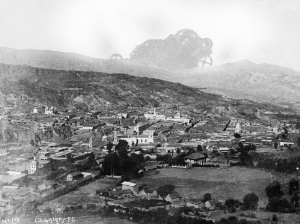
\includegraphics[width=0.5\linewidth]{images/SCP-001-the-broken-god-7.png}
	\caption*{SCP-001的较早图像,在附近城镇的撤离中拍摄}
\end{figure}

于1943年7月17日,全球超自然联盟的特工联系了基金会在墨西哥拉巴斯的主管,请求支援对001-登神实体所在地的运输。基金会特工迅速部署飞机救援GOC人员。抵达后,特工描述称他们获得一个特殊的异常器物,并有可能被用于阻止001-登神实体行动。

在抵达拉巴斯的三天后,于1943年7月24日,全球超自然联盟派出一名特工携带该特殊器物去往001-登神实体所在地。在1943年7月25日早上,在001-登神实体抵达太平洋海岸时另一个巨大的机械构造体\footnote{之后编为SCP-2399并在文件中给予合适掩盖故事。}出现在其上方。该实体的来源未知。

在SCP-2399出现后的事件记录不完整且可能不准确。此次遭遇的结果是SCP-001被消灭。SCP-2399消失,之后以损坏状态出现在木星,当中原因至今未知。

SCP-001剩余的非活跃部分,即一团巨大分散的机械部件,留在了加利福利亚海湾底部。在从非活跃的结构体中取出SCP-882后,剩余部分坍塌彻底停止活动。

在001-登神事件后,对该区域居民进行了代号“下加利福利亚”的大规模记忆删除行动。此次行动因SCP-001周围厚重的黑烟得到支持,当前历史记录将此事件描述为一次森林火灾。大量精力被投入在修正区域地图及搬迁失所平民上。出于对大规模记忆删除规范的需要,多个实验性神经变形器被使用\footnote{特别是U级、UN级和UP级记忆删除,当前都已被终止。},因对其副作用缺乏认知,估计此举造成不少于200万人在001-登神事件后的十年内死亡。

\bb{附录001.10:}收集到的全球超自然联盟文档 \\
\ii{备注:下列文件由POI-004D/001(参见附录001.12)交予基金会人员。当前未知POI-004D/001如何获得此文件。}

\begin{tcolorbox}[colframe=black, boxrule=0.5pt, colback=white, center upper, leftright skip=0.12\linewidth, breakable]

\begin{figure}[H]
	\centering
	
\includegraphics[width=0.6\linewidth]{images/SCP-001-the-broken-god-8.png}
\end{figure}

ATTN:Darius将军

物品回收报告

\bb{编写:}Van Pelt中尉

\bb{C.O:}Baghram上校

\bb{报告长度:}57页

\bb{报告概要:}1942年12月30日,一个具异常性的游荡人形实体在希腊海岸外的小岛附近被巡逻员发现。该实体,宣称没有名字也不能流利用英语交流,携带一个棒球大小的小型立方体器物。实体似乎为女性,其头皮上连着几根钢链。

实体最初愿意交出所带器物(编为AR-213),但很快出现敌意并开始说话。实体对中队人员发出生命威胁,击倒两名人员,随后被Dixon军士制服。实体提及墨西哥西部,要求将其释放把该器物带去那里。

更多调查发现SCP基金会在该区域的活动越发频繁,同时还有一些轻微地理异变。在aghram上校指令下,第二团看守该实体(编为EN-340)开往异变地点。在舰船停靠美国边境后,EN-340开始变得消极,显然不适且心理失常。

建议返回后,在处决前对EN-340进行更多心理评估。一旦对AR-213的分析完成,器物将被送往苏黎世焚毁。

报告附于此以供考察

Lt. R. Van Pelt

第二团

全球超自然联盟维和部队

\end{tcolorbox}

\bb{附录001.11:}Ruberson特工的陈述,1944年1月

\ii{备注:特工Aaron Ruberson在收集SCP-001器物时正驻扎在站。因大部分基金会高级人员被派往参加收集,他被要求进行事后陈述。报告原先存放在 Site-17,之后被加入另一与SCP-001相关的机密材料中。未知是否有其他人员知晓此报告,或者有任何副本被制作。下面是陈述摘录。}

\begin{figure}[H]
	\centering
	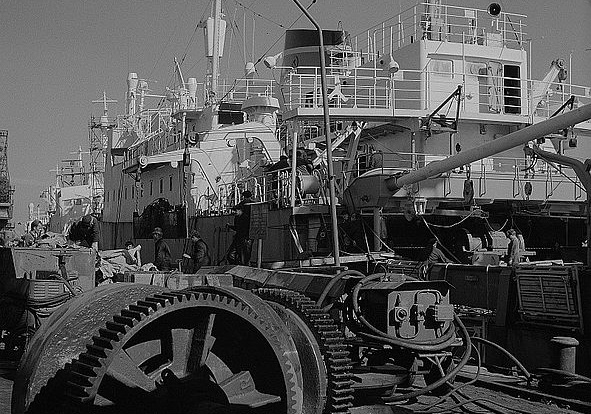
\includegraphics[width=0.5\linewidth]{images/SCP-001-the-broken-god-9.jpg}
	\caption*{SCP-001的非活跃部件正在被装船送往收容。}
\end{figure}

\begin{scpbox}

我们先把能从海岸拿走的拿了。小东西、齿轮滑轮还有活塞,就这一类。大部分都是垃圾,但还在抽动和旋转。它们还是有生命的。这些小零件大概在几小时后死透,但几周后我还是能听到那些大碎片在搅合。就像砍掉鸡头那样。

重要的部分,那些已知是真正教会器物的,被我们打包运往拉巴斯的列车运走。我数了数,基督啊,也许得有一百个?每个都是异常器物。车站有些小伙子笑话说就为存这些东西他们怕是得修个新站点。

幸运的是我们把伤亡压得很低。大部分人都只是在机械附近有些懵,就像是不能把手臂拿开一样。Rodriguez的手被压了,我们只好把他送去当地诊所处置。我觉得整个过程里就有一起死亡。一个我们雇来的当地人帮忙潜到海湾下给那个心脏捆上绳子,好让我们把它拉出来。我没看到,但我听说了。说他们发现他的头被碾烂在两个活动部件中间。还说看起来他是自己把自己推进去的。

但我不知道,我没亲眼看见。我倒是有看到标签。

你知道的,当某地制造了什么产品,为了便于辨认其产地,这些家伙总会找个大片金属刻上名字然后在部件一侧给它贴上吧?我们在其他部件上看到了不少这种东西,都是它在一路向海吃过去的途中收集的。不过教会器物都不是这样。它们和其他所有东西一样嗡嗡响,但是没有标志。你站在这些东西前就能感觉到什么,像是安详。整个感觉就像,它感觉很平静。像是解脱。

除了那个心脏。当我们终于把它搬上海湾,因为天气原因我们把它留在岸边放了一天。有些当地人开始发痒。说他们听到声音,不愿意靠近。不管多少钱都不干。只有等到北边的基地派来更多支援才能把它弄上船。

我…伙计我不知道。我见到过各种的这些东西,但我的模因抗性还是很高的。我为这个任务通过了不少测试,一切良好。但我无法抵抗围绕那心脏的另类感觉。我不知道可不可以说听到了什么,但…好吧,标签。我们把它搬上船向北准备离开的时候我第一次看见了。我那时候还没想到要说什么,甚至都没往心里去,知道我看到了其他一些文件。接着船在风暴中沉了,我们丢失了心脏,整个时间我一直在想着那该死的金属标签。接着我想我发现了。那根本不是教会的东西,Johnny。
标签上写的是“工厂所有”\footnote{因近距离检查SCP-882的困难性,这些言论尚未得到证实。}。

\end{scpbox}

\bb{附录001.12:}对POI-004D/001的采访 \\
\ii{备注:下面是2009年对POI-004D/001的采访摘录,此人自称为一此前未知的破碎之神教会分支成员。联系在特异事故调查单位协助下进行,他们曾与POI-004D/001有过互动,详情记录在附录001.01中。}

\begin{scpbox}

所以,给我说说你觉得你们知道的事。

明白了。

有趣。

好吧,你们倒也不是全错。在现在这个时候也是值得称赞的。我感觉你们忽略了几个关键细节,以及高看了某些自认健忘症患者给你们的情报。

那就让我直说好了。

GOC并没有杀死耶和华,虽然他们自傲地如此宣称着。他们消灭的也不是破碎之神。确实,那确实是它的碎片之一,但你会给我个轮轴再把它叫成车么?噢,所以你们把几个部分凑在了一起。也许有引擎了,但仍然不是车。

神比那要更为简单。神是万物。从最大的星到最小的尘。每个小部分,对它们自己都是微不足道的。做着它们应做的事。切合在一起,相互咬合。这全都是宇宙机械的一部分。

这机械的面貌,在某种程度上,就像是一种比喻。一个理念。但我肯定你们也知道,理念是强大的。它们从无中创造出有,或是将已有的加以改变。神的一小束火花闪过,象征成为真实。在一颗生命如此丰盛的星球上,你们产生了无数理念。

你可能要问,“为何要叫它破碎之神?”可能的回答有几个。和翻译问题一样简单的事。被虔信者重新解释得具体了。“破碎”只是对某个更微妙词语的糟糕翻译吗?神是在大爆炸中破碎了吗?如果是这样,它为何破碎?若它被修复又会怎样?

这些问题我一个都无法回答,但你们已经有了答案。到最后,无论神曾经是什么都不重要了。重要的是,对你们而言,它必须保持现状。“破碎”。神知道。那些更强大的部分,传统教派视为圣物的机械部件,它们知道它们本不该成为一个整体。就算迫使其合体,用异己的力量驱动,它们也知道自己本真为何。怪兽的啃咬会向自我毁灭行动,派出更小的实体来完成工作。GOC没有杀死它,它们是从它自己手中接过了枪,扣动扳机后又宣布这是自己的功劳。

问题在于,人类作为神的一部分太过渺小,无法去记忆。无法记忆他曾经是怎样。于是那些如Bumaro的人就要发明新路把我们推向奇点。

因为这是将要发生的。你可看到毁灭者的下部?在43年的遭遇前那里就是损坏的。如果你仔细看去,你将看到伤疤离动力核心越来越近。这次它甚至伤到了让它能藏进现实夹层的什么东西。最后那怪兽将胜利。它迟早会毁灭毁灭者,吞噬它,然后用它的力量吞食一切。我是说一切。神将后回归到唯一的完形存在,一个奇点,然后碎裂。只有这次它可能有了某种异己力量在其中。工厂之锈。Daevite王之血。第五教会,Wondertainment,街上随便某个有足够火花成为现实扭曲者的人。它们也会参与宇宙的重塑,并完结所有这些的次轮回。

不,这并不令我困扰。这是注定之事,这必将发生。谁又能说这不是已经在发生了,而你们的人是赢家呢?也许人类自身才是赢家。但这并不意味着我要反对关掉它,让主轮回继续。

是的,这有可能。我知道上次你们未能伤到那怪物,毁灭者也许到下次需要它的时候仍不能修复自己。但谁说你们不能支援它呢?或者模仿那些寻求重筑神明的人,得到外来协助呢?一同努力,没有什么不可能。

分离,我们是破碎的。但团结,我们将为神。

\end{scpbox}


\input{part00/001.past.and.future}

\chapter[SCP-001 一致意见]{
	SCP-001 Wrong - The Consensus \\
	SCP-001 一致意见
	\footnote{编者\QIS:这个脚注用于去除一个我还没搞明白的\TeX 排版问题,只要标题的最后一个字不是汉字就行,为了美观就加了个脚注\label{foot:fix}}
}

\label{chap:SCP-001.the.consensus}

\definecolor{ftwoftwoctwo}{HTML}{F2F2C2}

\begin{scpbox}[colback=ftwoftwoctwo, center upper]

\bb{基金会记录与信息安保管理部通知}

一年二度安保更新:项目编号随机化已启动。直至安保更新完成,所有文件将锁定。要进行紧急更新,请访问紧急数据归档系统(EDAS)。

— Maria Jones,RAISA主管

\end{scpbox}

\hr

\begin{scpboxcmd}

> 1908个项目存留。项目编号“SCP-001”锁定。 \\
> 识别到1个带有搜索字段“SCP-001”的文件。

> 文件~'SCP-001'被选中。 \\
> 开始自动项目编号随机化。 \\
> 扫描带有搜索字段“SCP-001”的文件…

\end{scpboxcmd}

\hr

\begin{figure}[H]
	\centering
	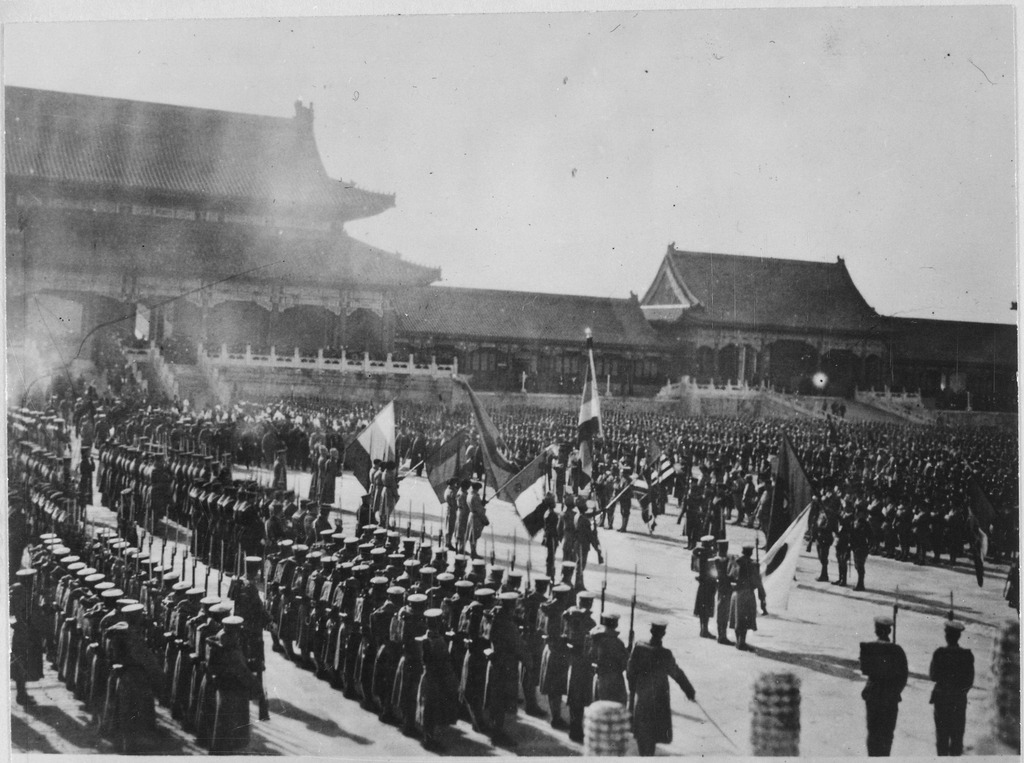
\includegraphics{images/SCP-001-the-consensus.jpg}
	\caption*{北京紫禁城,\red{SCP-001}的定义及紫禁城公约的通过在此完成。}
\end{figure}

\bb{项目编号:}\red{SCP-001}

\bb{项目等级:}Euclid

\bb{权限分级:}5级

\bb{特殊收容措施:}\red{SCP-001}当前无法被便利控制或收容,未知其是否会在未来发生。因此已采用应对方案。该方案由紫禁城公约的以下章节组成:

\begin{enumerate}
\item 依照紫禁城公约章节I,预防并最小化可能造成\red{SCP-001}或类似事件的情形。
\item 在紫禁城公约章节I实施后,依照紫禁城公约章节II及III安排组织过渡及联合。
\end{enumerate}

上述紫禁城公约章节不得变动,除非得到O5议会全体一致通过。

描述:\red{SCP-001}是一已经发生的CK级重构情形,造成过往某一迭代的现实变化,生成了当前的现实。从第一人称观察记录来看,\red{SCP-001}发生于前现实的公元1900年6月1日。\red{SCP-001}致使所有关于超自然大战\ii{i}(前一现实中称其为第五次超自然大战)的因果、事件、记载和记忆被删除并替代为各种异常或非异常的平行记录。

基金会关于超自然大战\ii{i}的文件采集自十三名非异常人类的传闻记录,这些人员因被称作“部分性\red{SCP-001}免疫”的现象而保有对前一现实的记忆。部分性\red{SCP-001}免疫的原理未知,依照O5议会指令不会对其进行评定。依照O5议会指令,对其他具有部分性\red{SCP-001}免疫人员的辨识工作被无限期暂停。

下面是在超自然大战\ii{i}中的事件及其在当前现实中可能的对应类似事件;参见文件OWi获取完整列表。

\tred{+ 查看列表}

\tred{- 隐藏列表}

\begin{longtable}{m{0.2\linewidth}m{0.3\linewidth}m{0.35\linewidth}}
\hline
超自然大战\ii{i}事件 & 描述 & 当前现实对应 \\
\hline
\endhead
\hline
\multicolumn{3}{r}{\small{接下页}}
\endfoot
\hline
\endlastfoot
“第五次超自然大战”的称谓 & 发生于公元19世纪的全球性战争,由发生于欧洲(拿破仑战争)、东亚(狄瓦族征服战)及美洲(美国内战)的三起独立冲突组成。战争中公然使用异常物体,造成了一次IK级全球文明崩溃情景。 & 与“拳乱”同时发生于中国北部的冲突事件,起义组织义和团据称在此事件中使用了某种未命名异常。\par 虽然对异常的使用非常微小,O5议会仍在知晓异常现象的诸组织中倡议将“第五次超自然大战”作为对此事件的正式称呼,全球超自然联盟在基金会-GOC的1953年峰会中正式承认了这一主张。\\
拿破仑一世加冕 & 拿破仑皇帝在加冕后宣布新诺斯替教为法国国教,欧罗巴为国家守护神。& 教皇庇护七世将拿破仑加冕为“法兰西皇帝”拿破仑统治期间从未有发现过新诺斯替主义和欧罗巴女神崇拜的表现。 \hyperref[chap:SCP-2515]{SCP-2515}是对此的唯一证据。\\
狄瓦族东亚征服战	& 东亚大部分地区被名为\overtextnote{\hyperref[chap:SCP-140]{狄瓦族}(\footnotesize Daevites)} 的类人文明入侵。征服从中国黑龙江省及吉林省开始。& 没有对应事件。\hyperref[chap:SCP-140]{SCP-140}中的记录显示狄瓦文明被蒙古人消灭于公元13世纪。然而,确实曾在中国黑龙江省及吉林省发现过狄瓦文明器物。\\
南北战争 & 美利坚合众国及美国南部邦联间的内战。名为“工厂”的团体向双方都提供了异常军备支援。在南部邦联政府转移后,战争逐步扩展到墨西哥、中南美。& 未发现工厂参与南北战争。战争规模始终局限于美国大陆地区。\\
图基教平定运动 & 第零反邪教军团针对骚扰\hyperref[chap:SCP-2833]{Vātula}(被视作与英国东印度公司对抗狄瓦族对印度入侵的共同战力)的犯罪集团图基教的镇压活动。& 由《1836-48年图基教及土匪镇压法案》委任的镇压活动,确认有新欲肉教参与。\\
梵蒂冈神秘及预言圣裁庭 & 知晓异常现象的组织,隶属于梵蒂冈圣座。在拿破仑进攻意大利半岛时,其成员逃难到南美、非洲自由邦及中东。& 圣物部(梵蒂冈圣裁庭下属部门)叛逃到意大利统一政府,组建了基金会前身组织之一“皇家基督教圣物办公室”。\hyperref[chap:SCP-1732]{梵蒂冈圣裁庭在公元1964年与基金会合并}。\\
“墨西哥帝国”的建立 & 自称Cem Anáhuac,是阿兹特克帝国的后继者。\hyperref[chap:2155]{其对象及由其产生的媒体具有模因能力},被用于政府周边邦国,如德克萨斯、危地马拉、萨尔瓦多和洪都拉斯。& 墨西哥第二帝国在法国干涉下建立,由皇帝马西米兰一世统治。据传他在被处决前曾与一个SCP-2155-1个体安排了联姻。\\
东田纳西会议 & 由东田纳西的合众国支持者组成,在田纳西州参与南北战争后脱离该州。由此形成的\hyperref[chap:SCP-1328]{富兰克林州}被承认加入美利坚合众国,也是合众国一方中唯一一个自南部邦联脱离的州。& 东田纳西会议在南方军占领东田纳西后告终。西弗吉尼亚自弗吉尼亚州脱离,并在南北战争后作为一个州保留。\\
太平天国运动 & 在狄瓦占领下的中国南部发生,由一名为洪仁坤的奴隶策划发起,他自称得到了名为\hyperref[doc:2481]{“龙母”}的神明启示。在起义首都太岁京(被太平军占领前为南京)被狄瓦族攻陷后遭到镇压,全城居民被屠杀。& \hyperref[chap:SCP-089]{SCP-089}告知的一起S级事件,由女王陛下超常控制收容基金会及黑庄园的联合探险队处置解决。洪仁坤在此利用了对基督教的自我改造,并给自己改名为洪秀全。\par 未发现欲肉教或基督教相关异常活动涉及此事。南京在被太平军占领后改名为天京。\\
土默特部大屠杀 & 一名狄瓦族奴隶在狄瓦占领下的蒙古地区系统性屠杀了150000名蒙古人。报告称\hyperref[chap:SCP-076]{此奴隶}手持两把带刃武器并具有某种再生能力。起义者的尸体被狄瓦军队以未知目的回收。& 一起“金丹道之乱”类似地造成了150000名蒙古人被屠杀,但此事是由中国秘密结社金丹道造成。金丹道在前一现实的存在因资源有限而无法确认。
\end{longtable}

\red{SCP-001}的起因和源头未知,也无法确认。未知\red{SCP-001}或类似事件在此之前是否还曾发生,也未知其是否会在未来发生。此外,未知\red{SCP-001}是否是CK级重构情景的典型或非典型表现。若\red{SCP-001}或类似事件已经发生或是将要发生,推测大部分(甚至全部)人类和/或智能实体将对此事件及其发生前的事件不会保留记忆。无法确认部分性\red{SCP-001}免疫是否能在未来的\red{SCP-001}或其类似事件中有效。

\red{SCP-001}的定义由O5议会以投票5-4-4完成,紫禁城公约于公元1901年9月7日签订。

\bb{附录1:}紫禁城公约摘录

\bb{章节I:基金会}

\begin{whiteboxbb}

下列组织将自各自资助方中解散并脱离关系,其人员及资源将进行合并:

\begin{itemize}
\item 女王陛下超常安保收容基金会
\item \ii{黑}庄园
\item 沙皇先知会
\item 德意志帝国秘传战团
\item 美国安保收容倡议
\item 帝国侵犯事件委员会
\item 皇家基督教圣物办公室
\item 荷兰东印度公司特别调查董事会
\item 内阿非利加探索队会社
\item Borja y Aragón军备骑士团
\item 阴阳局
\item 中华异学会
\item 第零反邪教军团
\end{itemize}

它们将被取而代之联合为一个统一组织。

该统一组织的使命是控制并收容各种异常事物,以保护人类免受此类事物威胁。

同意将该统一组织的称谓定为“基金会”;其他替换称谓(如“学会”、“组织”、“机构”、“前哨”)曾被提议但否决。上述十三个基金会构成组织自此后称作“基金会前身组织”。

\end{whiteboxbb}

\bb{章节II:O5议会}

\begin{whiteboxbb}

基金会的临时执行管理部门将是来自各前身组织的十三名人员组成的执行议会。

上述十三名执行议会成员将依照下列标准选择:

\begin{itemize}

\item 在各基金会前身组织居领导职位
\item 保有关于第一次超自然大战\ii{i}的记忆

\end{itemize}

未来的执行议会成员不再要求满足上述两个要求。

同意将执行议会的称谓定为“O5议会”;其他替换称谓(如“监督者委员会”、“5级议会”、“O5指挥部”)曾被提议但否决。

O5议会的功能将为促进各前身组织间的初步过渡。

每名O5议会成员将以罗马数字编号,从一排列到十三。

今后其他并入基金会的组织机构不得在O5议会存有代表。

\end{whiteboxbb}

\bb{章节III:关注组织}

\begin{whiteboxbb}

知晓异常现象存在而不受基金会管控的各组织机构被编为 \overtextnote{“关注组织”(Groups of Interest)}。

基金会对各关注组织的默认对策是促成其人员和资源的解散、终止和/或将其吸收。

\end{whiteboxbb}

\bb{附录O5-(1-13):}继任笔记re:\red{SCP-001}。 文件根据登录的O5账号显示。

\definecolor{dafadnine}{HTML}{DAFAD9}

\begin{scpboxc}[colback=dafadnine]

验证登录权限。识别到管理员优越权(代号嚎叫黑月)。\\
展示所有文件。

\end{scpboxc}

% \begin{whiteboxbb}

\begin{scpbox}

欢迎您O5-1

致我的继任者,

作为\red{SCP-001}的主要编辑者,我已写下了你所需知晓的一切。在\red{SCP-001}后,只有我们十三个知道它,我们各自代表各自的前身组织。当然,我们命定要指挥和联合为基金会。

你可以从我们的投票看出,我们在北京争论时有关于\red{SCP-001}的另外两种版本。它们最终被投票否决,但二和十二仍在基金会历史上留下了自己的记号。遗憾的是十二有限的英语水平让它选中了相对通俗化的分级名词,与二和我刚好相对。无论如何,我们召开首次O5会面的倡议将在已写下的所有SCP文件中被记忆、发扬。

至于基金会之使命,我希望你和你的同事能继续我们的工作。

\end{scpbox}

\begin{scpbox}

欢迎您O5-2

致我的继任者,

桑塔亚纳曾说,“忘记过去的人必将重蹈覆辙”。现在,整个世界都忘记了过去。但它会重蹈覆辙吗?它会的。

在第二次世界大战期间,不是又有一个威权独裁者恐吓欧洲,中国人再一次被屠杀了吗?当然,细节些许不同,美国也在战争中保持了完整。也许内战在你的一生曾再次发生,或者很快就要发生。又或者缩减为一次小冲突。 工厂仍然留存,但它只是幻影。

异常的产物自身也会是异常。\red{SCP-001}和它的世界不是例外。一点一点,世界在毁灭、重蹈覆辙。每有一个SCP不(或者只是最低程度地)在我们的控制下,这个进程都要继续。在那之前,系统里都会有混乱存在。曾经,我提议指引世界回到原来的状态,但其他人不愿赞成专横暴行。最终,我认了。 没必要为我的观点斗争。没什么能改变这个过程。

除了等待,不必采取任何行动。或者简言之,“Keter”。

\end{scpbox}

\begin{scpbox}

欢迎您O5-3

致我的继任者,

异常与正常—都取决于合意。今日的异常可能是昨日之正常,反之亦然。九未能发觉的丑闻就是一例;出逃狂在合意认为它不再成立后便不再是异常。

将合意适用在\red{SCP-001}。对其余的世界,超自然大战从未存在。它们只对那些知道异常的人存在。对知道异常的人,超自然大战\ii{i}并不存在。只有十三人幻想它存在,那可能就是\red{SCP-001}。

然而,议会建立了我们自己的合意,我的观点在它宣告之时也随之转变。我们多数决定应该对所有异常事务建立管控秩序,而不是觉得我们自己才是问题。这只是第一批达成的合意之一,我们能左右世界将什么视作正常,什么不是。也许是他们造就了你所成长的这个世界。

所以,请记得这些。合意有其价值,要正常就要被合意所接纳。

\end{scpbox}

\begin{scpbox}

欢迎您O5-4

致我的继任者,

只有少数人在两个第五次超自然大战中都上过前线,我是其中之一。我对官方的第五次超自然大战非常失望,毫无疑问那是缩了水的。那些拳匪根本无法与狄瓦族和发条信徒相比。就算是把几乎其他所有机构、教派都变成了我们的敌人,地下结社无论如何不能与全面战争相比。

也许这又是我心头的年轻热血在抱怨。\red{SCP-001}发生后它频繁的发作,就像在北京我一时冲动投票支持了二的提议。我并不关注他古怪的理论。我只想战斗。已经做出了如此多的牺牲,我也做出了惨重牺牲。不能让它们结束在这平静的日子里。但现在,我老了,平静也快找到我了。但你在此继续战斗。别让它在平静中终结。

\end{scpbox}

\begin{scpbox}

欢迎您O5-5

致我的继任者,

你现在知道了这世界曾经因为一起无法控制的事件而免于彻底毁灭。而正因其不可控制,我们无法保证它不会再次发生。或者会不会如我们愿地发生。我们不能依靠\red{SCP-001}这样的不确定。

作为一个物种,我们已经主宰百兽,踏遍大地。许多技艺已为人所掌握,而它们曾经都只是幻梦。世界的复苏只是另一件有待主宰的事情。若世界能让自己倒带,我们也能做到。

在我们的联合之下,我所展望的\hyperref[chap:SCP-2000]{杰作}将可能成为现实。它可能已被利用过,或是建构仍在继续着,但\red{SCP-001}一旦就绪就将不可逆转。凭我们的意志,人类将主宰永恒。

\end{scpbox}

\begin{scpbox}

欢迎您O5-6

致我的继任者,

我们同意\red{SCP-001}曾经发生, 但我们不知道这是否是\red{SCP-001}唯一一次发生。它会不会再次发生?一定要世界濒临毁灭才会出现吗?要到什么程度才足够?这跨现实的记忆保留又是为何,这是怎么回事?为什么是我们?它能复现吗?问题表如此继续。

这非常现象的不确定级别显然需要得到量化。‘Euclid’是对此的提醒,即对于\red{SCP-001}还应当有更多了解。我想你应当有此动力,毕竟有着基金会倡导科学方法论的熏陶。收容与保护不能是终点;知识才是。但第一届议会的大部分人害怕探索,想着要么抛弃它要么预防。哪一种都不能真正解决问题。

但你可以为解决问题做自己的贡献。只有你能看到这些,并访问到我仅有的少许发现,所以就让它成为你的出发点。愿你得到结果,为\red{SCP-001}带来有意义的资料。

\end{scpbox}

\begin{scpbox}

欢迎您O5-7

致我的继任者,

官方而言,只有13个人对\red{SCP-001}免疫。但还有另外一人,Jibril Mani。他是为土耳其皇廷工作的一名顾问,我在因拿破仑逃难到君士坦丁堡期间遇到了他。他无比好客,我们很快成了朋友,尽管基督教世界和伊斯兰世界历来敌对。我们待在一起直到\red{SCP-001}来临,突然之间我回到了罗马。

在现在的世界,他想办法找到了我,我知道他还记得我们曾经的友谊。我们在见面后大谈对超自然一战的记忆。我邀请他加入北京的聚会,和其他还记得战争的人一起,但他礼貌的拒绝了。

Jibril更愿意保护他的朋友和族人,特别是我们知道中东正一片混乱。他对一和他的势力心存怀疑,但我也无法为此责难他,只能尊重他的选择。那之后我们分道扬镳了。当我获得O5-7的头衔,Jibril告诉我他\hyperref[chap:ORI-oria.hub]{会回到伊朗召集自己的人手}。

就像他希望保护他所爱的人,我的使命是这世界,我会保卫他。

P.S. 出于尊重,我决定不对议会报告Jibril的事。我希望无论Jibril和议会最终各自成立了什么样的组织,它们都不要发生冲突。我们只愿保护。

\end{scpbox}

\begin{scpbox}

欢迎您O5-8

致我的继任者,

你可以从投票中猜到,对\red{SCP-001}的来头有过三个选择。一的提议无疑是唯一选择。其他人太愚蠢了。二基本上就想让我们去当无政府主义者,十二则觉得我们是一帮疯子需要服点东方神药。不必了,谢谢你们两个!

我们大多从一开始就在收集异常物件,所以基金会对多半前身组织而言并无多少不同。而对剩下的一半,关注组织的制度会让所有人意见一致的。

你应该已经做这些工作好些时候了,所以我希望你继续下去。

\end{scpbox}

\begin{scpbox}

欢迎您O5-9

致我的继任者,

\red{SCP-001}是现实的重构,这是我们的合意。所以\red{SCP-001}是现实扭曲。二宣称现实会不可避免地逆转回去以纠正世界,这和斯克兰顿在此问题上的著名观点颇为相似。不过,后者认为这种复原是由现实扭曲者引发的。控制智能存在可能非常困难,虽然某些学者认为一台\hyperref[chap:GOI-grant.request.for.the.manufacture.of.devices.to.regulate]{引擎}也许可以在理论上提升概率。这种前景带来了希望-这已知最庞大的现实扭曲活动是可逆的。

而当此事发生,世界真的复原到之前的状态-和我在非洲自由邦、并未真正受到IK级情景波及的家园一起完成。它可能也是过往世界里唯一安全的避风港。这样的稳定在\red{SCP-001}之后失落了,最终我要在一片更不友好的条件里工作。

虽然我并不喜欢一的观点,基金会目前到确实是更好的环境。这是个思考如何实现斯克兰顿想法的好地方,或者至少资助有这能力的某人。尽管我已投入了财力人力,进程依然缓慢,我已接受了事实,我可能再不能拿回所失去的东西了。

但你能,如果\red{SCP-001}再次发生。你应该继续用你所能的方法研究下去, 你不应该像我这样失去了自己的东西。没有人应该这样。

\end{scpbox}

\begin{scpbox}

欢迎您O5-10

致我的继任者,

十三个团体一起创立了基金会,但并非我们每一个都地位平等。比如十二所代表的异学会并未得到清朝的承认。而我这边也同样在走下坡。我们的名号属于一位猎巫人,但我们从未见过真正的女巫。19世纪末的Borja骑士团说成是关注组织会更恰当。要不是我对超自然大战\ii{i}的记忆,它就会一直如此。

当一说出他的大计划,我却对如何对抗异常心存怀疑。每一代骑士都是前一代的影子,结果如何呢。在超自然一战中,我记得我的骑士们被拿破仑的发条兵全歼。他们过去(现在也是)并未准备好迎接超自然之战,或者是对抗恶魔及法师。接受一的提议意味着再一次送他们惨烈赴死。作为他们的大团长,我不能送他们去死。

当投票结果不合我意,我曾差点考虑不签署合并条约。但当我听到八提议促进我们新命名的基金会联合起来,这种想法便烟消云散。那之后,我决定我的骑士们至少应该有意义地在与怪物的战斗中死去,而非作为牺牲品。

我们所有人终有一死。就让它对你责任之所在有所意义好了。

P.S. 其实考虑到这一切,其他前身组织的资源也确实能让最后一代骑士们比前一批更优秀。

\end{scpbox}

\begin{scpbox}

欢迎您O5-11

致我的继任者,

恭祝你为基金会服务。我想你是一级一级爬上这个位置的,而不是我这样因为品德第一上位。你的品德一定让人震惊,不同于我。

在超自然大战\ii{i}期间,京都陷落于狄瓦族之手,孝明天皇和议会大部分人罹难。将军和他的特务们逃去了虾夷。我是少数逃离京都的幸存者,但这只是因保命而胆怯。我最终为自己的选择悔恨,耻辱将我压倒。死不能令我解脱。至少孝明天皇在这新世界驾崩地要略微平和。

这决定了我在北京的投票,我们是出现了幻觉,记忆删除能治好我们。其实我只是想遗忘而已。但合意已成,我不被容许遗忘。一坚持我们命定要合作,议会里没有人站到我们这边。

知道还有人和我一样后,至少好受了些。三、七和十三带来了非常积极的影响。我的继任者啊,我并不了解你这一代O5议会的同事们,但他们将是你的忠实盟友。谨记。

\end{scpbox}

\begin{scpbox}

欢迎您O5-12

致余之继任者,

汝必尝闻除忆秘法,经年,其效亦有所\hyperref[chap:SCP-3000]{增},然回溯其源,实为基金会诸秘密之一也。余将释其原本。

除忆秘法者,初为孟族术师之密。余与彼族女约为婚姻以得之。初,余见幻景烦扰,欲以秘药去之,然今知其为超自然大战\ii{i}之记忆也。

未及药成,十一通信于我,曰有幻景类同。未几,余便知有外邦人若干见得同样幻景,且约为集会于京城。余身为医者本当见人病愈,便劝其勿为蛇足之举以求身全。然同会诸君不以为然,议以西洋民主投票之法定夺之。余之见自然为其所弃。

然除忆秘法不为其所弃。五以其略同于\red{SCP-001},可逆人之记忆,实为可用之方也。由是,除忆方不以余见为疗病之药,而用之于平民百姓见异事者,除其记忆。

有所不幸,孟族主母不容洋人窃其族方,余等遂将孟族一部列之于最初之关注组织。其一族下场大抵同于义和拳,但余一二小辈携一不甚解之\hyperref[chap:SCP-484]{秘方},奔逃香港。

汝自当效汝才干于议会,然既已谋得此职位,汝定当已效英才于此也。

\end{scpbox}

\begin{scpbox}

欢迎您O5-13

致我的继任者,

\red{SCP-001}说只有十三名前身组织的领导者才对其效应免疫,事实并非如此。只有十二人。

一和我已经认识了几十年,我欠他许多。自然,当他要我投下决胜一票,我答应了。他把狄瓦人入侵印度的事告诉给我以完成骗局。当那里都是我不知道的东西,我只会怪罪不列颠不愿对我的军团坦诚相待。

我想你现在该对这头衔为耻,我敢说我们这可能有三个不同的基金会在相互斗争。对我,这是让欧洲人正视问题、让我赢得优势的机会。自那时,我已作出许多补救,不让他人落入我的处境。

所以,向我保证你会以自己的意愿去投票,而非他人。

\end{scpbox}

% \end{whiteboxbb}

\hr

\begin{scpboxcmd}

> 扫描完成。识别到40个“SCP-001”。\\
> 开始随机编号生成…

\end{scpboxcmd}


\chapter[SCP-001 破晓之时]{
	SCP-001 S. D. Locke - When Day Breaks \\
	SCP-001 破晓之时
}

\label{chap:SCP-001.when.day.breaks}

\begin{scpbox}

你发现了那条通道,正隐藏在距主干道一英里外的天然洞穴内。

无需钥匙卡,通道之门是敞开的。

这里的气味闻起来和它们一样。但愿它们已经离开了。你走的太远,你无法回头了。

一条平滑的小径从洞口向内延伸,通向站点深处。也许会有些血液或粪便 – 或是那些东西涂抹的污渍,这可说不准。所以你得小心避开。

你仍能收到求救信号,它是从昨天开始的,无论是谁 – 你祈祷他们能够生还。

你的脚步声回响在空荡走廊之中,每一步都仿佛传达自另一个世界,就好像你并非在黑暗中独行。

电梯停留在底层 – 故而你沿楼梯下行,直至B5层:Keter控制区,你穿过几个空收容室,它们曾能造成的恐惧和动荡早已不复存在。

如果你运气够好的话。

这条路将你带往大厅一侧的办公室 – 那里正是信号的来源。门没上锁,但被什么东西卡住了,你抬起脚,用尽全力踹了过去。

在你能看清屋里的事物前有个东西从你左侧的角落里冲了出来,你的第一反应是“狗”。

但它曾蛰伏在天花板上。

你躲入房间,砰地关上身后的门。此处一片漆黑,你是安全的。你脱下外套,摘掉头盔。在经历了如此之多的事情后却死于中暑将会是莫大的耻辱。

唯一的应急操作灯旋转在塑料外壳之中 - 每隔一秒便在房间中洒下暖橙色的灯光,仿佛房间本身的脉搏正有节奏地律动着。

门后随意搁置着 – 一个路障,你环顾四周,脏衣服和吃了一半的食物,尽管临近厕所,角落里却有个盛满排泄物的桶。北面墙上的气动室将向房客提供必要的生活物资。

你的路终止于房间角落某个令人作呕的泥潭,你看到了三个药瓶 - 检查发现这是三种不同的鸦片类药物,它们都是空的。

桌上有台电脑,靠近终端,你可以清楚地看到电源指示键闪烁着微弱的灯光。

你坐下,开机。

\end{scpbox}

\hr

\cl{

\Gg{紧急协议激活。删除级别保护措施。完全访问权限。}

控制。收容。保护。

\par

\par

加载中...

加载中..

加载中...

加载中..

加载中...

加载中......

}

\begin{scpbox}
你听到门外传来了脚步声,一步步愈发沉重,下一步又接踵而至。
\end{scpbox}

\cl{

加载中...

加载中..

加载中...

加载中..

加载中...

加载中..

加载中...

加载中..

加载中...

正在验证...

..

...

}

\begin{scpbox}
黑影由地板和门边的缝隙悄然渗入,被光线映照地轮廓分明。
\end{scpbox}

\cl{

..

...

..

正在验证...

..

...

..

...

..

正在验证...

..

...

}

\begin{scpbox}
你紧张地屏住呼吸等待着,希望它只是路过。然而你的心跳此刻在你自己听来,却震耳欲聋地暴露了你的位置。
\end{scpbox}

\cl{

请等待...

..

...

..

..

...

请等待...

..

...

..

请等待...

..

...

..

}

\begin{scpbox}
阴影消失了,你的呼吸松懈下来,正在这时,屏幕亮了起来……
\end{scpbox}

\par

\cl{

打开文件

\Gg{🔥自动化安全系统通知代码235(ASSN-235)🔥}

检索SCP-001文件当前迭代时出错,您正在查阅版本\#3 ,可滑动至页面底部查阅较新版本。

}

% =====

\newpage

\tred{开启文件:SCP-001修订版\# 3/12:(1)音频文件}

\tred{隐藏修订版}

\g{\bb{修订版\# 3/12更新于1312日前}}

\hr

\begin{figure}[H]
	\centering
	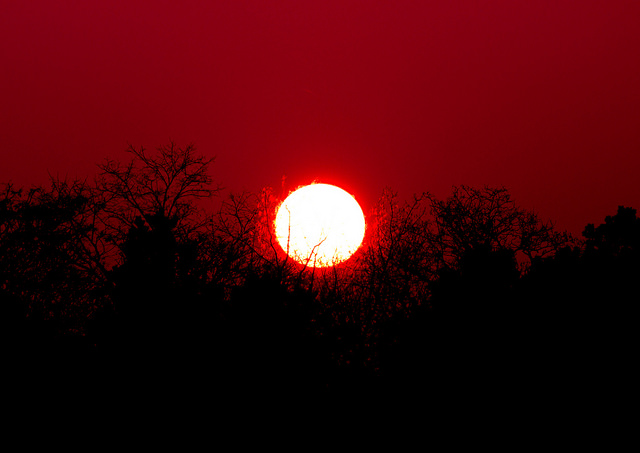
\includegraphics[width=0.5\linewidth]{images/SCP-001-when-night-breaks.jpg}
	\caption*{SCP-001激活后数分钟,拍摄者未知。}
\end{figure}

\bb{项目编号:}SCP-001

\bb{项目等级:}Apollyon\footnote{译注:abad,希伯来语意为破坏者,希腊语译为apollyon,英语译为abaddon,指圣经启示录中的地狱使者亚巴顿,又称无底坑的使者。}

\bb{特殊收容措施:}由于其性质,SCP-001无法被收容。SCP-001事件幸存者将驻扎在安全设施中并彼此保持联系,鼓励人员采取任何可行的手段前往Site-19。

希望进行户外活动的幸存者必须保证周身覆盖防护服;最好是多层防护,应尽可能避免徒步旅行,城市 – 也指通常意义上的人造建筑可提供最大程度的庇护,需规避树木繁盛区,空乘是所有出行方式中的最优选择。

暴露于SCP-001的人员将被视为损失,受连累者将被遗弃,请不要尝试安乐死。

应不惜一切代价避免SCP-001-A组成规模庞大的集群,已证实电导武器在固定情况下有一定作用,故可用于自卫,燃烧器也可正常使用,迄今为止,冷冻弹药是最有效的。

测试显示SCP-001-A是相对安全的可消耗品,但只能被视为没有其他选择的情况下的最后手段。由于SCP-001-A可在消化系统中重构,因此短时间内仅能消耗少量,以防止堵塞。

驻扎于Site-19的人员从事有关世界殖民化的研究,载具经过专门设计,内部不得被光线穿透。

\begin{scpbox}

\begin{scpbox}

对于那些失去了家人,或者上帝啊,失去了孩子的人们 – 我对此深感,深感遗憾。但你必须坚持下去,不要让他们白白死去,我们还有时间。

人类仍可能拥有未来,到Site-19来,我们需要尽可能多的援助。

学会拥抱黑暗,朋友们,我们惧怕光明。

\hr

\hfill - \ii{The Administrator}

\end{scpbox}

\end{scpbox}

\bb{描述:}SCP-001是在事件[系统错误]\ii{数据丢失:ec172,请联系系统管理员。}后对于太阳的编号。此次事件发生二十四小时内造成约68亿人类伤亡。SCP-001的影响似乎不是经由紫外线产生,而是暴露于可视光谱(~390至100nm)导致。即使身在月光下也同样如此。

当活体接触太阳产生的可见光时,将从接触点处开始液化,效果持续扩散,直至整个生物体完全转化。从外观上来看,同蜡融化类似。转化时间很大程度上取决于生物体的暴露程度和其大小。尽管发生了这种重组,生物体也不会死亡。

转化完成后,这些生物体(SCP-001-A)将呈凝胶状,它们会尝试活动,尽可能使自己固定在可令人联想起先前样貌的形态,这种努力可取得一定程度的成功。

植物通常保持物理惰性,但仍能够进行光合作用并产生氧气,可飞行的生物丧失飞行能力,动物具有意识,在未被吸收至集群的前提下,行为与往日无异。人类则保有少许智慧和记忆。

暴露于SCP-001的生物性异常受到同样的影响,曝光可抹消其曾表现出的全部异常。

由于它们的物质组成,SCP-001-A个体可通过彼此接触进行分子水平上的联接和混合,这似乎不会对个体造成任何痛苦和伤害,但组成的体积可抑制其运动。自SCP-001-A事件以来,大多数个体已集聚为这样的集群,似乎不存在最大融合上限。

融合后的生物质是无定形且混沌的,集群生物将在半液态中转换形态 – 其中肢体和身体质量将在短时间内周期性升高,随后恶化并被另一种生命形态纳入。

集群个体将使用它们的附属物来移动自身的质量,多数情况下它们会使用组织成分构建伪足,并以类似变形虫的方式拖动自己。

\cl{\red{
+打开附件:音频日志 \\
... \\
... \\
... \\
授予访问权限。
}}

\begin{scpbox}

当你打开文件时,扬声器中发出了刺耳的静电噪音,扰乱了房间的静谧,你措手不及,心跳加快。也有些噪音来自于调节麦克风。

沉默转瞬而逝:

\end{scpbox}

\begin{scpdialog}
“咳咳,这里是Logan Igotta博士,级别,嗯,三级研究员。”
\end{scpdialog}

\begin{scpbox}
她的声音有些颤抖,以至于听起来没有那么专业。她停顿片刻,深吸一口气,而后继续说道。
\end{scpbox}

\begin{scpdialog}
“由于Site-46拥有几个传染性信息危害 – 所以我们,我们启用停电协议将 – 将其余网络切断了,因此我们将使用新信息通道来传递现状。

从好的一面来说,我们实际上还能接收到来自其他几个站点的信息,似乎有相当数量的人这么做了,有些计划突破19,有些正试图冲击As,也有些,和我们一样,只是简单地等待时机。我们的站点暂时封闭,我们还没准备好旅行,至少现在还没有。
\end{scpdialog}

\begin{scpbox}
她叹了口气。
\end{scpbox}

\begin{scpdialog}

“几天前我们……遭遇了一次收容失效,一台类人型机器人失控了,这王八蛋放跑了半打,半打Keters。

在像碗浓汤似的崩溃前,它们没能跑出隧道五英尺远。我 – 我看着它们倒在凸轮上。

没过多久它们又重新站了起来。”

\end{scpdialog}

\begin{scpbox}

她再度停了下来,念诵着你难以理解的呓语 – 在你能够继续听见明确无误的语句之前。

她几不可闻地呼气。

\end{scpbox}

\begin{scpdialog}
“啊.……好,好多了,恰好在指定吸烟区;但是到底发生了什么,嗯?
\end{scpdialog}

\begin{scpbox}
她清了清喉咙。
\end{scpbox}

\begin{scpdialog}
“指挥官Anand穿戴整齐,第二天便去了镇上,试图去赶他们。事态没什么好转,可怜的混蛋。不过我们确实学到了一两件事。”
\end{scpdialog}

\begin{scpbox}
停顿,喘息。
\end{scpbox}

\begin{scpdialog}

“只有少数几个人离开了这里,我躲在办公室里,Herry和Phillips主任在营房的某处,Clyde和几个D级把自己锁在了军械库里,和Ari一起。

我真该去看看她要做些什么的。”

\end{scpdialog}

\begin{scpbox}
片刻间她哑了声 – 你听到无线电喋喋不休的嗡嗡声。
\end{scpbox}

\begin{scpdialog}
“嘿,嗯,你在那儿怎么样?”
\end{scpdialog}

\begin{scpbox}
一个声音回应了她,是个极为夸张、语调嘲讽的男声。
\end{scpbox}

\begin{scpdialog}
“我现在在这也就是照料 - !我要你知道我 - !呃,唔。”
\end{scpdialog}

\begin{scpbox}
Logan开枪还击。
\end{scpbox}

\begin{scpdialog}
“谁?谁呢 – 把它关掉,该死的我要跟她通话。”
\end{scpdialog}

\begin{scpbox}
另一端则传来喧哗声,收音机易了手。温柔而关切的声音正呼唤着。
\end{scpbox}

\begin{scpdialog}
“宝贝,怎么了?”
\end{scpdialog}

\begin{scpbox}
Logan回应道。
\end{scpbox}

\begin{scpdialog}
“没事 – 没事 – 什么都没有。”
\end{scpdialog}

\begin{scpdialog}
停顿,喘息。
\end{scpdialog}

\begin{scpdialog}
“我只想尽快确认一下。”
\end{scpdialog}

\begin{scpbox}
Ari恳求着。
\end{scpbox}

\begin{scpdialog}
“我很好,宝贝,真的,我能照顾好自己。”
\end{scpdialog}

\begin{scpbox}
咯吱声 – Logan转过座椅。
\end{scpbox}

\begin{scpdialog}
“不,不,我知道,我明白,我无能为力,我知道来到这儿对你来说很不容易……”
\end{scpdialog}

\begin{scpdialog}
“……一切事情都——”
\end{scpdialog}

\begin{scpbox}
Ari打断了她的话。
\end{scpbox}

\begin{scpdialog}
“嘿,你告诉我你戒烟了。”
\end{scpdialog}

\begin{scpbox}
短暂的噪音,也许是Igotta试图掐灭她的香烟。
\end{scpbox}

\begin{scpdialog}
“哦!呃……不!不,当然的,我的意思是,我戒烟了。”
\end{scpdialog}

\begin{scpbox}
Ari似乎并不相信。
\end{scpbox}

\begin{scpdialog}
“我想你并不需要担心我,我一直很干净,甚至这几个月都没想过碰致幻药。相信我。

无论如何,既然你想知道,我没事。小伙子们正围在扑克牌边,我和笔记本一起窝在角落里。”
\end{scpdialog}

\begin{scpbox}
你可以听到Igotta开玩笑似的笑了笑。
\end{scpbox}

\begin{scpdialog}
“亲爱的!在这样的时刻还想着要写首关于你我之间永恒爱恋的十四行情诗?我受宠若惊。”
\end{scpdialog}

\begin{scpbox}
Ari笑着回答。
\end{scpbox}

\begin{scpdialog}
“一首挽歌,如果我现在无法让自己沉浸在某事之中,一定会发疯的。”
\end{scpdialog}

\begin{scpdialog}
“我明白,嗯,我会尽快带你回来的。

我爱你。”
\end{scpdialog}

\begin{scpbox}
Ari回答。
\end{scpbox}

\begin{scpdialog}
“我也爱你,宝贝。”
\end{scpdialog}

\begin{scpbox}
片刻的寂静,通讯中止,而后又是一声几不可闻的叹息。
\end{scpbox}

\begin{scpdialog}
“我们只剩下这些人了,其他的要么在事件中丧生,或是死于收容失效。主任命令我们原地待命,继续盯紧凸轮 – 那里面的还有设施附近的,001跳跃在我们的门前,天知道我们这儿还锁了什么东西。

电力仍在运转 – 我们还能维持相当长的时间 – 而且这里有足够多的物资能够维持数年,我们能过得很好。”
\end{scpdialog}

\begin{scpbox}
停顿,喘息。
\end{scpbox}

\begin{scpdialog}
 “一切都会好起来的。” 
\end{scpdialog}

\begin{scpbox}
传输结束前,她等待了几拍。
\end{scpbox}

\hr

% =====

\newpage

\tred{开启文件:SCP-001修订版\# 5/12:附加事件报告}

\tred{隐藏修订版}

\hr

\g{\bb{修订版\# 5/12更新于1202日前}}

\begin{figure}[H]
	\centering
	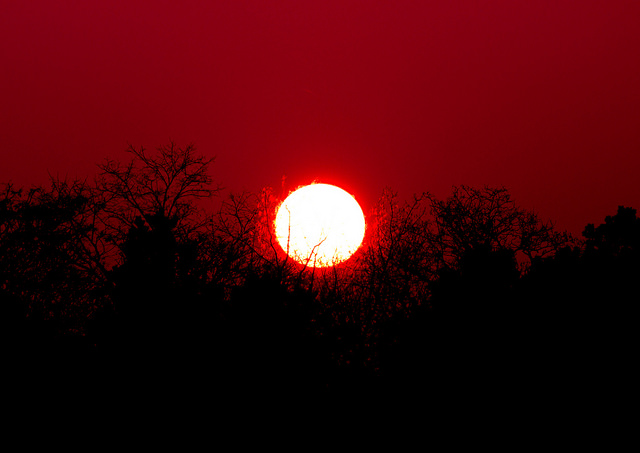
\includegraphics[width=0.5\linewidth]{images/SCP-001-when-night-breaks.jpg}
	\caption*{SCP-001激活后数分钟,拍摄者未知。}
\end{figure}

\bb{项目编号:}SCP-001

\bb{项目等级:}Apollyon

\bb{特殊收容措施:}\red{未提交更改。信息崩溃。}

\bb{描述:}\red{未提交更改。信息崩溃。}

\cl{\red{
+打开附件:事故报告-001.1\\
...\\
...\\
...\\
授予访问权限
}}

\begin{whitebox}[left=2pt, right=2pt, top=2pt, bottom=2pt]

他们一直坐在那里,呼唤并乞求我们走到外面去。噪音引来了更多人。这样庞大的一个集群,我敢肯定至少有几十个人,天晓得里面混杂了多少动物。尖叫、抱怨、怒吼和咆哮声此起彼伏,简直比地狱更响亮。最糟糕的是令人恶心的呻吟声 – 就好像他们真的在享受似的。

他们只要知道我们还在这里,就不会离去。

我们设法说服了一个D级出去看看 – 看他能不能把它们引开,他的计划令人惊讶 – 他只要了一把手枪,和一颗子弹。他走到它那儿去,随即它捉住他试图掀开他的面具,他设法将枪口抵住下巴然后扣动扳机。我想他很幸运。

他踉跄地跌倒在地,它滑进了他的防护服,撬开面罩,从内部开始将他撕裂。

他回来了;开始转化 – 曾是他身体的凝胶从衣服中滴落,尖叫尖叫尖叫。

它们甚至不让我们寻死。

主任有个计划,他的办公室里有个逃生隧道,站点下方的电车可以将我们带到一个安全屋 – 我们应该可以从那里起步,前往Site-19。

\end{whitebox}

\hr

% =====

\newpage

\tred{开启文件:SCP-001修订版\# 8/12 一(1)附件}

\tred{隐藏修订版}

\hr

\g{\bb{修订版\# 8/12更新于1200日前}}

\begin{figure}[H]
	\centering
	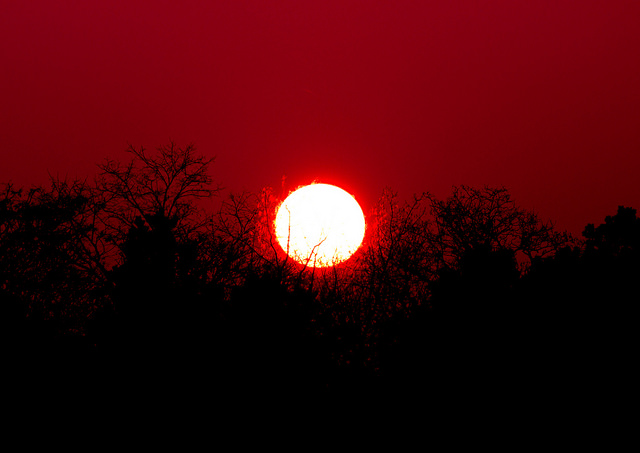
\includegraphics[width=0.5\linewidth]{images/SCP-001-when-night-breaks.jpg}
	\caption*{SCP-001激活后数分钟,拍摄者未知。}
\end{figure}

\bb{项目编号:}SCP-001

\bb{项目等级:}Apollyon

\bb{特殊收容措施:}\red{未提交更改。信息崩溃。}

\bb{描述:}\red{未提交更改。信息崩溃。}

\cl{\red{
+打开附件:音频文件\\
...\\
...\\
...\\
授予访问权限
}}

\begin{scpbox}

你第一次看到她的样貌,Igotta博士坐在你现在所处的地方,神情痛苦,双眼布满血丝,胸口处晕染着大而潮湿的黑红色。

她颤抖而短促地呼吸着,嘴唇翕动,似乎是在说话,声音却哽咽在了喉咙里。她垂下头,无声地啜泣起来,一分钟后,她设法克制住自己:

\end{scpbox}

\begin{scpdialog}

“我,我 – 我们,电 – 电车……

在隧道里,从天花板流淌下来,拖动,拖动他们进入,光 – 光剥开他们的衣服,和,和 – 和……”

\end{scpdialog}

\begin{scpbox}

她将手伸入胸前的口袋,掏出半截断指,断口下方可清晰地看到结婚戒指的暗淡光泽。她紧紧握着它,捧在手心里,拇指摸索着闪烁的金属。

她近乎永恒地呆坐着,反复低声道歉,乞求宽恕,看起来失魂落魄。片刻后她抬起头来,发现自己还在录音,好像回归了现实;她将断指塞回口袋,前倾身体,像是要关闭摄像机,但是这时一台收音机发出了声音。

它播放了几秒白噪音,而后突兀地传出了令你万分紧张的声音。

\end{scpbox}

\begin{scpdialog}
“Logan?”
\end{scpdialog}

\begin{scpbox}
那几乎是Ari的声音,然而那声音已经受到影响、如肠鸣音一般。Logan错愕地张开嘴,脸庞血色尽失。
\end{scpbox}

\begin{scpdialog}

“你在哪儿?为什么我回不到里面去?

你在吗”?

\end{scpdialog}


\begin{scpbox}
Logan从办公桌下捡起一部手持式收音机,她的手有些颤抖,那东西不断恳求着她;不成人声的嗓音让你倒尽胃口。
\end{scpbox}

\begin{scpdialog}
“宝贝,没关系,\ii{我}没事,真的。

这是个明亮而阳光灿烂的好日子,你却无所事事地虚度光阴。”
\end{scpdialog}

\begin{scpbox}
Logan泪流满面,手指盘旋在呼叫按钮上方。曾是Ari的东西用一种深沉而湿润的声调呼吸并说话。
\end{scpbox}

\begin{scpdialog}
“多么美丽而澄澈的蓝天 – 和那天一模一样,你还记得吗?”
\end{scpdialog}

\begin{scpbox}
Logan用她空闲的手拿起一支烟,而后划着火柴。她哆嗦着手指两次尝试点燃烟头却失败了。她在心底默默宣誓,第三次点燃香烟,吸了四分之一。曾是Ari的东西继续说:
\end{scpbox}

\begin{scpdialog}
“这太完美了,和我一直梦想着的一模一样,你的计划真是精巧,我从未像此刻这样感受到爱。”
\end{scpdialog}

\begin{scpbox}
Logan开始摇晃。
\end{scpbox}

\begin{scpdialog}
“甚至有乐队演奏我们的歌谣……”
\end{scpdialog}

\begin{scpbox}
它开始歌唱。
\end{scpbox}

\begin{scpdialog}
\ii{“我感觉很好,以这特殊的方式}

\ii{我坠入爱河,这是个阳光明媚的好日子”}
\end{scpdialog}

\begin{scpdialog}
Logan将收音机丢出房间,它在某处磕碎了屏幕,但仍在运作 – 你仍能听到那东西的歌声。
\end{scpdialog}

\begin{scpdialog}
\ii{“好日子,阳光明媚的好日子}\\
\ii{好日子,阳光明媚的好日子”}
\end{scpdialog}

\begin{scpbox}
随着无线电慢慢消逝,越来越多的声音齐声合唱,几个,几十个,乃至更多,他们放声歌唱,直到收音机仁慈地沉寂下去,Logan从她的椅子上跳起来冲了出去,你可以听到她在屏幕外呕吐。视频画面定格在空座位上,过了几分钟,她返回并关掉了摄影机。
\end{scpbox}

\hr

% =====

\newpage

\tred{等等,哪里不对。}

\tred{…}

\begin{scpbox}

有种挥之不去的、却又似妄想的感觉包裹着你,你正被监视。你戒备地睁大眼睛,尽管视线从显示器处移开后需片刻来适应黑暗,应急灯光扫过房间,将阴影拉伸扭曲地面目全非。这时,你发现了它。

在那儿,在那角落中。

它正从泥潭中爬出。

时间在这一刻放缓,一双手,涂满了遍布整个设施的黑色粘液,撑在了令人作呕的泥潭两侧,仿佛地板下方的东西正努力支撑,试图将自己的身体抬升起来。

不成人形。

头部随之而来,从粪便中上升,乱蓬蓬的毛发遮盖了它的脸,不明液体肆意横流,它转向你的方向。

它在角落中注视着你,而后再次沉入黑暗。

应急灯光再次穿过房间,扫射着泥潭,它看起来和方才别无二致。

\end{scpbox}

% =====

\newpage

\tred{开启文件:SCP-001修订版\#9/12 一(1)附件:}

\tred{隐藏修订版}

\hr

\g{\bb{修订版\# 9/12更新于986日前}}

\begin{figure}[H]
	\centering
	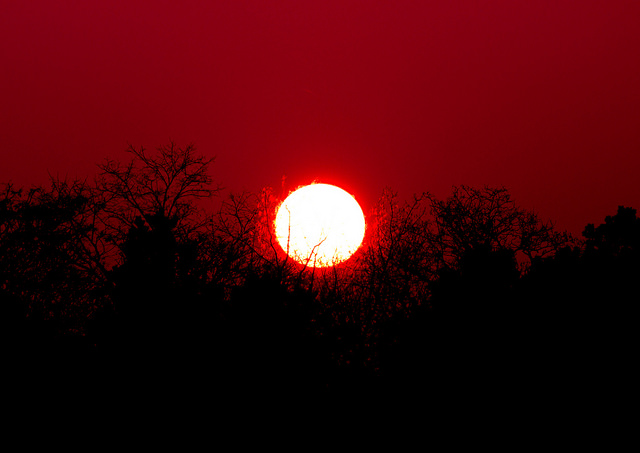
\includegraphics[width=0.5\linewidth]{images/SCP-001-when-night-breaks.jpg}
	\caption*{SCP-001激活后数分钟,拍摄者未知。}
\end{figure}

\bb{项目编号:}SCP-001

\bb{项目等级:}Apollyon

\bb{特殊收容措施:}

\bb{描述:}\red{未提交更改。信息崩溃。}

\cl{\red{
+打开附件\\
...\\
...\\
...\\
授予访问权限
}}

\begin{scpbox}
Igotta博士的身影出现在显示器上,她看起来消瘦了,大张的双眼遍布血丝。桌面上搁着一把刀,一只碗,一页表面泛黄的马尼拉信封。

上面叠着一卷染血的羊皮纸。
\end{scpbox}

\begin{scpdialog}
“虽然我们身处基金会,并且面临了这些事情,但我一直认为我们能够保持控制与收容,我们将隐匿于黑暗之中 - 令人类在光明的大道上蓬勃发展。

Site-19的通讯上月起中断了,我越来越难以找到理由坚持下去 – 尤其是,在失去了……”
\end{scpdialog}

\begin{scpbox}
她抓起刀,犹豫了片刻。
\end{scpbox}

\begin{scpdialog}
“那些声音一次又一次地在我脑海中盘旋飘荡,我时常回忆起隧道中的那天,一切事情都发生了。我已经回去过几次了,只是为了能再次听到她的声音。

但这是错误的,门那边的东西 – 不是她,她再也不会回来了。那声音听起来很像她,它也知道她所知道的一切,但它不再是她了。这光 – 它夺走你的身体,偷窃你的思想。

但你的灵魂呢?”
\end{scpdialog}

\begin{scpbox}
说到这儿,她将刀片压入左手掌心,因疼痛而抽搐。你看着她握紧拳头,令血液流入碗底
\end{scpbox}

\begin{scpdialog}
“如果这样做……能让我寻回失去的,光线无法企及之物;我会回来更新的。现在我说完了。”
\end{scpdialog}

\hr

% =====

\newpage

\tred{开启文件:SCP-001修订版\# 17!24ATA错误}

\tred{隐瞒我}

\hr

\g{\bb{修订版4847/3RR0R更新于985日前}}

\begin{figure}[H]
	\centering
	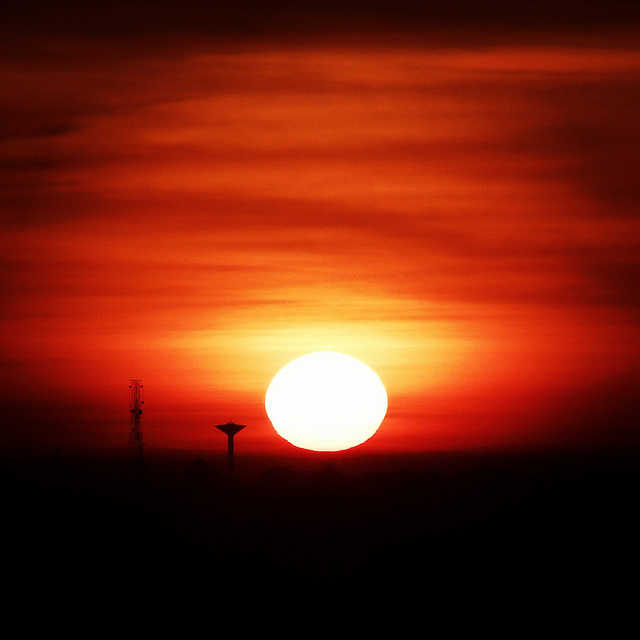
\includegraphics[width=0.5\linewidth]{images/SCP-001-when-night-breaks-2.jpg}
	\caption*{它是多么温暖。}
\end{figure}

\bb{编号。}伤害。

\bb{项目。}Apologize

\bb{特殊收容措施:}SCP-001\bb{不应}被收容,SCP-001事件幸存者将驻扎在安全设施中并永远无法彼此保持联系,鼓励人员\bb{克服自身,停止思考他们所知之事。}

\bb{你不可能永远隐匿此处,吾爱。}

暴露于SCP-001的人员将\bb{不可}被遗弃,我没有要求你救我,这不是你所做的选择。 请\textsuperscript{
不要不要不要不要不要不要不要}尝试安乐死。

已证实电导武器\bb{为什么?}在固定情况下有一定作用。\bb{你无法忍受我变得更好。}燃烧器\bb{如同瘙痒。}迄今为止,冷冻弹药是最有效的。

驻扎在Site-19的人员将\bb{不遗余力,我也是,永远不会太晚,宝贝。}

\bb{描述:}SCP-001是\bb{我们终获自由后}对于太阳的称谓,其影响是瞬时的,\bb{将将你从所有痛苦中解放, 直至你将我撕裂。这种变化看起来很吓人,我明白,}尽管经历了这种充足,但你\bb{不会死。}

\bb{我保证。}

由于它们的物质组成,SCP-001-A个体可通过彼此接触进行分子水平上的联接和混合\bb{并最终以这种形态存在}。这不会造成\bb{任何痛苦}。自SCP-001-A事件以来,大多数个体已集聚为这样的集群,似乎不存在最大融合上限。\textcolor{white}{不要担忧}

所得的生物质是\textsuperscript{美}\bb{丽}\textsubscript{的},集群中的生物体将在其内部和周围游移,\textsubscript{进入}\textsuperscript{分离}\textsubscript{进入}\textsuperscript{分离}\textsubscript{进入} - 其中肢体和身体部分都将转移\bb{永不放弃}。 \textsubscript{万物归一}随后恶化并被另一种生命形态纳入。

集群中的个体仅是想要再度靠近你。

如此努力。\\
\small{让我进入}

\g{\bb{带我回去}}

\begin{scpbox}

附有一个视频文件,打开它,你将看到它拍摄者你所身处的房间,画面似乎来自一个设置在房间角落的监控摄像头。环境十分昏暗,但你可辨认出Igotta博士,躺在远处墙边堆放的衣物上。

她在睡眠中不安地扭动身体,似乎正承受着折磨和伤害。她辗转反侧,嘟囔着无意义的音节。

摄像头抖动,微微向上抬起,而后再次重点关注她。

它开始缓慢靠近。

扬声器开启;你听到了轻而平缓的呼吸,随着摄像头靠近博士,这声音愈发清晰,逼真。不仅仅是白噪声,而是又几十个 – 几百个声音共同组成的含糊不清的耳语。

你靠了过去,几乎将耳朵贴在了扬声器上,试图弄明白它们在说什么。由不一致声中脱颖而出的却是:

\end{scpbox}

\cl{
你在注意?\\
下一幕便是为你而设。
}

\begin{scpbox}

不过你不太确定该怎么做,回顾显示器,镜头已停顿在距睡着的博士差不多一英寸之处,

噪声停止了。

悄无声息。

一只手,黑而油腻,且瘦骨嶙峋,伸向她的前额,撩开了一缕头发。

她猛地睁开眼睛,震惊地反击,视频切断了。

\end{scpbox}

\hr

% =====

\newpage

\tred{开启文件:SCP-001修订版\# 9/12一(1)附件:}

\tred{隐藏修订版}

\hr

\g{\bb{修订版\# 12/12更新于1日前}}

\begin{figure}[H]
	\centering
	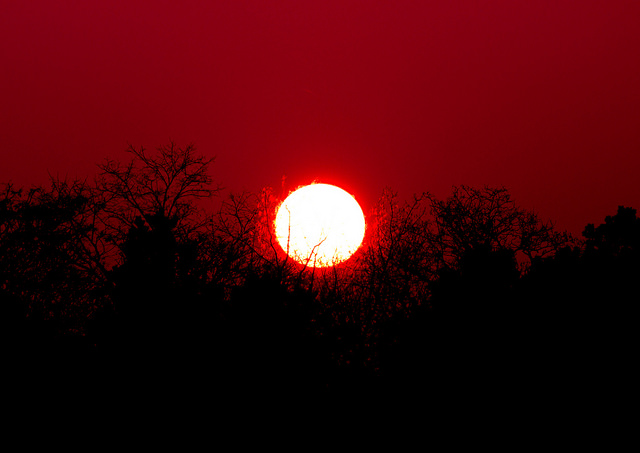
\includegraphics[width=0.5\linewidth]{images/SCP-001-when-night-breaks.jpg}
	\caption*{SCP-001激活后数分钟,拍摄者未知。}
\end{figure}

\bb{项目编号:}SCP-001

\bb{项目等级:}Apollyon

\bb{特殊收容措施:}\red{文件恢复于此前版本。信息崩溃。}

\bb{描述:}\red{文件恢复于此前版本。信息崩溃。}

\cl{\red{
+打开附件\\
...\\
...\\
...\\
授予访问权限
}}

\begin{scpbox}
Igotta博士出现在画面中,状态看起来比以前更加糟糕,头发明显稀疏,中间缺了大片。若不是正反射着显示器的柔和光芒,你甚至会以为她不再拥有双眼,因为它们已深陷入了她的眼窝之中。她眼睛一眨不眨地凝视着前方。
\end{scpbox}

\begin{scpdialog}
“她不会停止,她,她从未离去,我知道我没有,没有因浏览文档感染信息危害。我测试自己是否受到-4673感染,答案是否定的。-5189是,是唯一,唯一使用打印作为载体的,不 – 不是,我仍拥有全部的手指!”
\end{scpdialog}

\begin{scpbox}
她咧开双唇,露出一个破碎的笑容,她微弱地笑着,露出颤抖的双手,似乎曾是手指的骨骼遗骸大部分嵌入了她左手的血肉之中 – 支撑着她无名指处的残肢。两枚婚戒松散地套在上面,彼此相碰。
\end{scpbox}

\begin{scpdialog}
“所以,我没有感染,我不是,没有,我,我没有发疯。我知道,我知道仪式如何运转,我知道这真的是她,是她的,她——”
\end{scpdialog}

\begin{scpbox}
有些东西使她的注意力离开屏幕,她转首听着。
\end{scpbox}

\begin{scpdialog}
“不!不,我不 – 不能!你不是,不是你,这不一样。不是你,这再也不是你了,不!不不不!
\end{scpdialog}

\begin{scpbox}
她用力揉着自己的太阳穴,一遍又一遍地重复道。一分钟后,她转回头,面对摄像机。
\end{scpbox}

\begin{scpdialog}
“它是她又不是,我所带回的 – 仍然是一部分,没办法,束手无策,无可挽回。

未来对我来说毫无希望,上帝啊,我不能再这样下去了。

我在这儿很安全,光线无法到我身边 – 我,我不 – 不会让它,让它带走我。
\end{scpdialog}

\begin{scpbox}
她挥舞着一把手枪。
\end{scpbox}

\begin{scpdialog}
我本来计 – 计划用这个,直到我找到了剩下的,剩下的药物。我不想冒险,冒险将它们的注意力转移到我 - 我的身上……我的身体。
\end{scpdialog}

\begin{scpbox}
她拉开办公桌的抽屉,放好手枪,抬起眼皮凝视着摄像头。
\end{scpbox}

\begin{scpdialog}
妈妈,爸爸,Ari。

我很抱歉。”
\end{scpdialog}

\begin{scpbox}
她前倾身体,记录结束。
\end{scpbox}

\hr

% =====

\newpage

\tred{太可怕了}

\tred{就这样结束了吗?}

\begin{scpbox}
你拉开抽屉,抽出手枪,心不在焉地在手里翻弄了一会儿,想知道你该到那里去。Site-17?64?当然你不会是最后的幸存者。电脑发出声响,文件有更新吗?
\end{scpbox}

% =====

\newpage

\tred{访问SCP-001:当前迭代更新于一(1)分钟前}

\tred{__}

\hr

\bb{项目编号:}

\cl{
\ii{炽日升上了藏红花似的天空\\
偶然地相逢,彼此不安地表现\\
终有一日,吾爱,我们二者将}
}

\bb{项目等级:}

\cl{
\ii{融为一体,进程就此开始\\
浓雾迷乱而狂野,闪耀光辉;\\
旭日的光芒四射于湛蓝的晴空}
}

\bb{特殊收容措施:}

\cl{
\ii{就在我们奋力奔跑之时\\
穿越隧道,狂野的热潮,\\
那日,吾爱,我们终将拥有}

\ii{共度的未来 – 我们所赢得的生活\\
承诺与责任,为我们组建的家庭\\
蔚蓝的天空埋葬了闪耀的}
}

\bb{描述:}

\cl{
\ii{阳光,被命运淹没 – 超支\\
愤怒与怨恨肆意滋生\\
昨日,吾爱,你我尚为一体}

\ii{此刻你静卧于此,你的生命已离去\\
徘徊于她射线外的黑暗\\
绯红的天幕在火炬下烧灼;我们的太阳,\\
今日,吾爱,我们融为一体}
}

\begin{figure}[H]
	\centering
	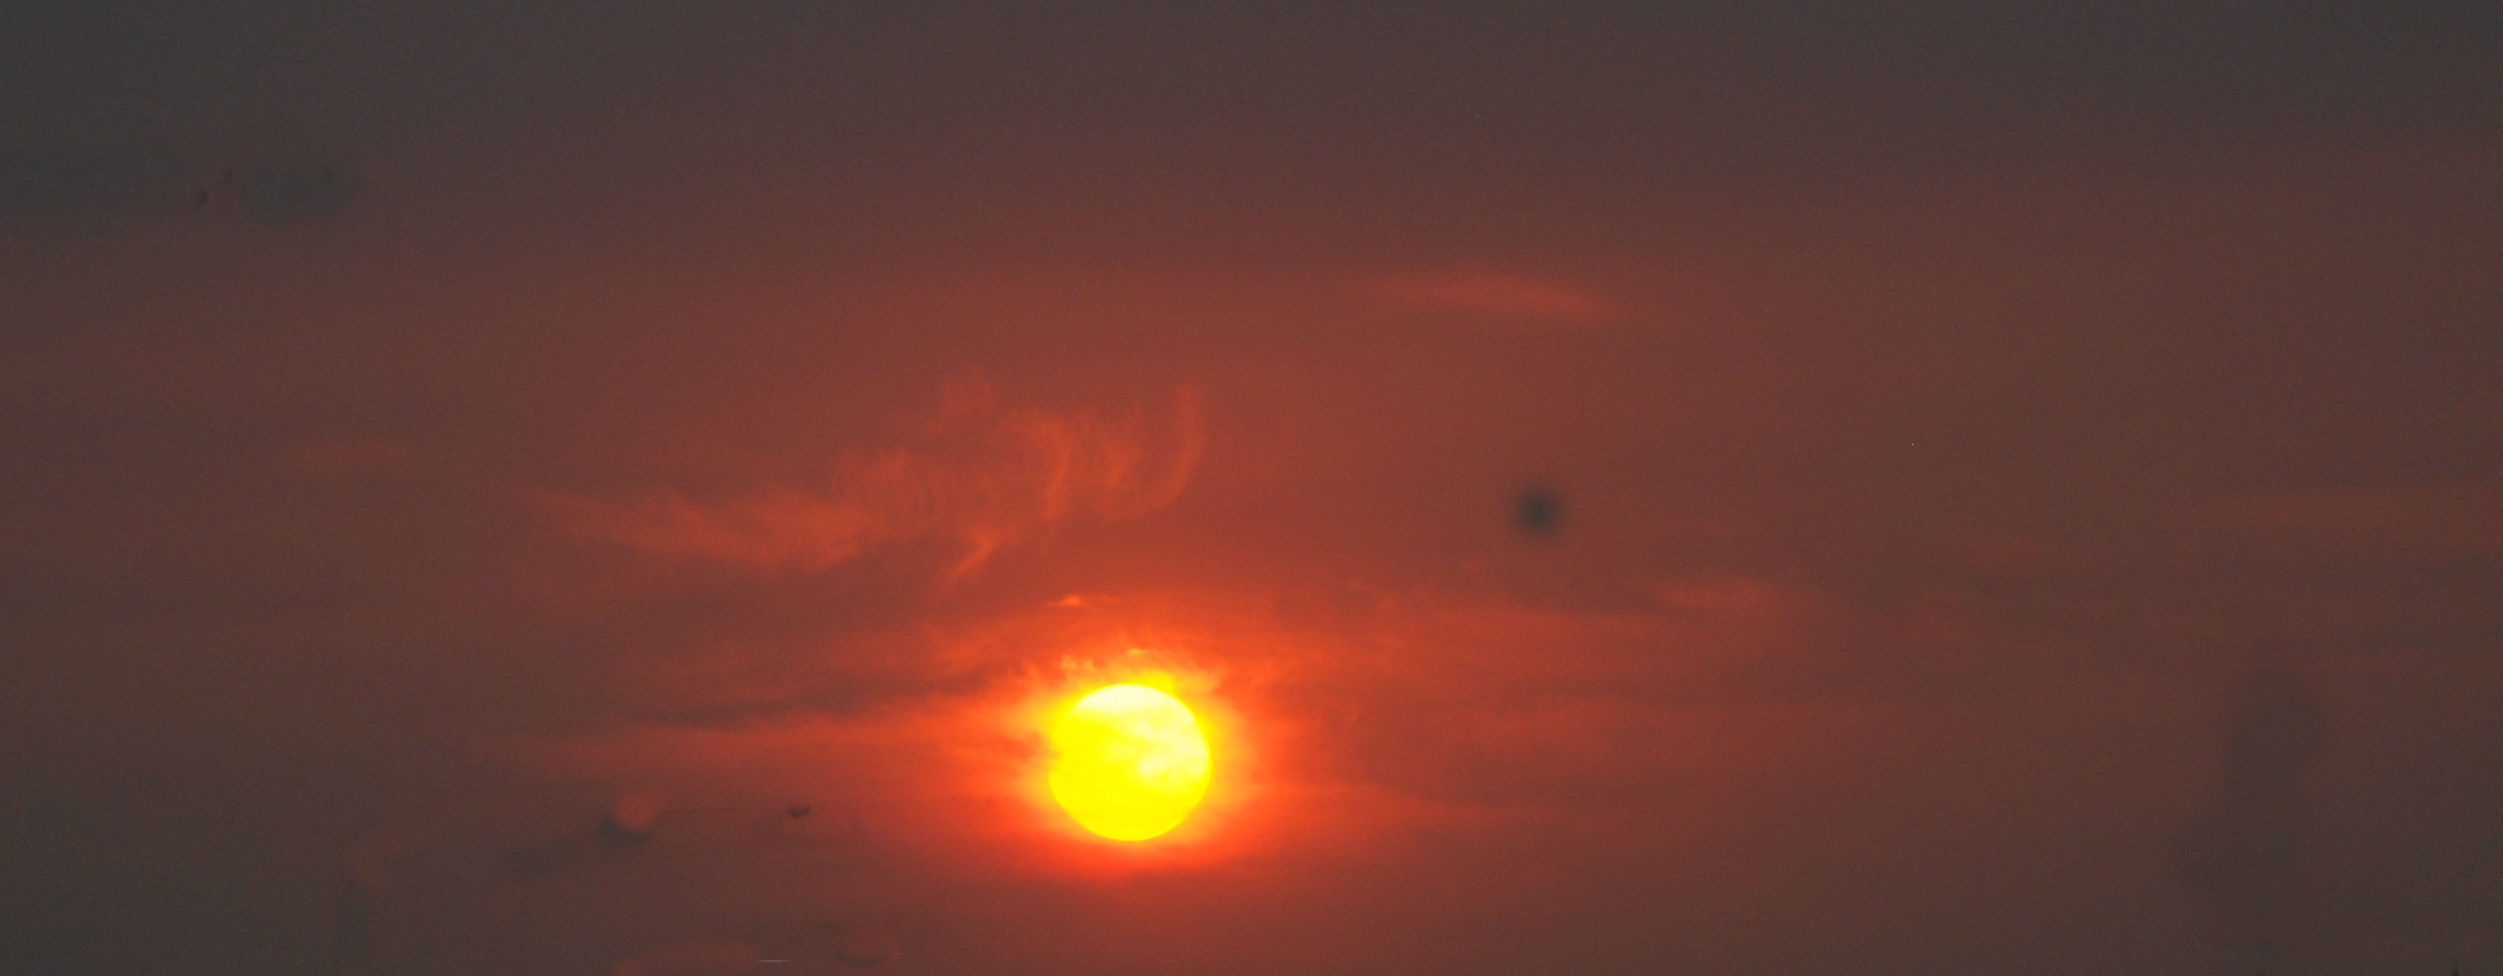
\includegraphics[width=0.5\linewidth]{images/SCP-001-when-night-breaks-3.jpg}
	\caption*{系统错误误误误误误误误误\# @\& \# .}
\end{figure}

\hr

% =====

\newpage

\begin{scpbox}

没有你的命令,显示器开始自动播放视频文件,当你看到加载出的图像时,寒意涌上心头。

这是一幕实时录像,来自你的背后,距离大约一英尺远。

一只骨瘦如柴的墨色左手进入画面,极缓慢地接近你。它没有无名指。

再来不及思考更多,你疯狂的转过身来举枪射击,希望能驱散幽灵。

你的子弹射入一面空荡荡的墙壁,此处一无所有。

在你听到它之前,有什么东西再度经过 – 在你听到它们的声音之前。流淌着的湿润的抨击伴随着尖声合唱涌入走廊。

它撞击着屋门,此处莫不是藏身之所?

它再度撞击,似乎有一张脸浮现出来,某一部分属于人类,其余部分则……是某些东西 - 正从缝隙中缓慢灌入。血肉从神知道由何而来的淤泥中渗出,重新组合成手指、眼睛与羽毛。

第三次。它此刻正压在木梁上,沉甸甸地使之向内下垂。

伴随着呻吟与破裂声,木梁支离破碎,门打开了。

手掌和臂膊拉起你,一个接一个地将你传递出去,经由空的收容单元,继续向上,穿过楼梯间,通往大厅和隧道。

你所拥有的宝贵黑暗不过片刻。

隧道的尽头,有光。

\end{scpbox}


\chapter[SCP-001 上帝的盲点]{
    SCP-001 God's Blind Spot\\
    SCP-001 上帝的盲点
}

\label{chap:SCP-001.gods.blind.spot}

\bb{项目编号:}SCP-001

\bb{项目等级:}Yesod

\bb{特殊收容措施:}T设施,基金会O5议会总部所在地及附属管理机构已围绕SCP-001所在地建立,包括SCP-001内的T-01号楼。T设施安保协议记录于文件T-001:01。

\begin{figure}[H]
    \centering
    \includegraphics[width=0.5\linewidth]{images/SCP-001-gods-blind-spot.jpg}
    \caption*{\bb{T设施}}
\end{figure}

\bb{描述:}SCP-001是一不规则形状空间,面积约65000平方米,包括地上和地下两部分,位于西奈山███████。除了其奇术性质(见下),SCP-001没有特殊之处,物质与能量可以自由出入其中。法国科学与艺术委员会在18世纪后期进行的考古研究表明此地有一石头建筑,可追溯到公元前2000年,类型符合住宿旅馆。由于T设施的建造,此原本建筑遗迹已无留存。

SCP-001的特殊之处,在于其为目前地球上已知唯一一处天然的Akiva辐射绝对零环境。实验已证实即便将Akiva辐射源引入SCP-001空间范围\footnote{参见研究报告SCP-001.08.P(佛陀齿遗物),1974。}的周围或内部此情况仍会维持,这表明并不仅是SCP-001的外边界严密阻隔了Akiva辐射穿过,SCP-001本身也在吸收和消灭发生于其内部的Akiva辐射。

作为SCP-001性质的结果,智人对象认知功能与器官功能的自然劣化、终结过程会在对象身处SCP-001边界内时中止。换句话说,在特定条件下,人类不会在SCP-001中死亡。参见下列测试记录:

\begin{longtable}{m{0.15\linewidth}m{0.6\linewidth}m{0.15\linewidth}}
\hline
\multicolumn{1}{c}{测试} & \multicolumn{1}{c}{参数} & \multicolumn{1}{c}{结果}\\
\hline
\endhead
\hline\multicolumn{3}{r}{\small{接下页}}
\endfoot
\hline
\endlastfoot
01.001 & 人员D-1082,健康人类男性,安置在SCP-001内部的标准收容间内,观察120天。 & 无变化。\\
01.003 & 人员D-2326,健康的人类女性,安置在SCP-001内部一气闭容器内。向容器内注入致命剂量氰化物气体,测试完成后将气体排出。 & D-2326未出现有害医疗问题。\\
01.006 & 参数同于测试01.003,但对象为30只健康的大白鼠(\ii{Rattus norvegicus})。 & 对象死于氰化物中毒。变体测试表明SCP-001的维生效应仅限于人类对象。\\
01.009 & 人员D-5337,患有4阶段癌症的人类女性(转移到大部分器官),预后其将立即死亡,将其安置在SCP-001内标准收容间中,观察786天。 & 无变化,身处SCP-001内期间对象的癌症症状无任何恶化。对象在测试结束离开SCP-001后的48小时内死亡。\\
01.010 & 人员D-5361,健康人类男性,将其安置在SCP-001内的焚化炉中然后启动。 & D-5361的身体如正常受控程序一样燃烧。其残骸没有特别之处。变体测试表明SCP-001的维生效应没有包括到全部类型的伤害。\\
01.338 & 人员D-8874,健康人类女性,安置在标准SCP-001内标准人形收容间中并被束缚。将对象的左腿在无麻醉下于大腿处截断,且不使用麻醉或止血带等束缚股动脉的措施。在截肢后,其断腿被移出SCP-001,对人员D-8874进行360天的观察。 & 对象暂时失去意识(可能是由于疼痛及突然失血)但恢复,流血在12小时内停止。截肢处快速愈合。移出SCP-001的断腿正常分解腐烂。\\
01.537 & 人员D-13926与D-13927,健康人类男性双胞胎,年龄24岁。D-13926安置于SCP-001内的标准长期人形收容间,D-13927安置在其他基金会设施的长期人形收容间。对象被观察26年零10月。 & 人员D-13927表现出正常的生理变化进程,而D-13926在测试期间没有出现明显衰老。测试结束后D-13926被送往其他基金会设施,这之后对象出现了加速发生的衰老变化。
\end{longtable}

已在T-01号楼内建造了居住设施,可供基金会O5议会全体成员和其他高级管理人员生活居住。当前,12名O5议会成员中有9人居于此宿舍内,此9人中的8人自T-01号楼建造完成起便再未离开。\footnote{第九位O5成员离开T-01号楼处理个人事务,在预定返回前遭气象事件杀死。}

因SCP-001的性质,其也被用作基金会奇术研究计划的控制站点,包括\hyperref[chap:SCP-2336]{SCP-2336-A个体}的应用开发。

\bb{归档文件06-S7INF-23-A(摘录)}

\begin{figure}[H]
    \centering
    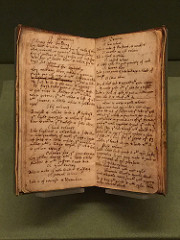
\includegraphics[width=0.5\linewidth]{images/SCP-001-gods-blind-spot-2.jpg}
    \caption*{\bb{手稿“对上帝实质的观察”(艾萨克·牛顿爵士)基金会收藏品。}}
\end{figure}

\begin{scpbox}

…在自然哲学和对全能上帝本质的问题上,我们必须凭着感官的证据开展探究,包括神圣经文的证词。虽然无人曾见得上帝,然而对上帝之感知可来自观察他的创造,及至对神圣经文的细致研究。

思考出埃及记第四章,以希伯来文写是:

\usefreeserif{ויהי בדרך במלון ויפגשהו יהוה ויבקש המיתו׃}

\usefreeserif{ותקח צפרה צר ותכרת את־ערלת בנה ותגע לרגליו ותאמר כי חתן־דמים אתה לי׃}

这,将其翻译,是说:

\ii{摩西在路上住宿的地方,耶和华遇见他,想要杀他。西坡拉就拿一块火石,割下他儿子的阳皮,丢在摩西脚前,说:“你真是我的血郎了。”}\footnote{出埃及记4:24–26}

思考这些诗篇的教导。许多饱学学者将关注点投于诗篇第二段,这里西坡拉,摩西之妻,施行割礼,且,以此做法,解救她的丈夫免于全能上帝的怒火。在此,学者们说,是一种道德教诲,告诉说没有人,即便是上帝的先知,得以豁免于他的约法。

但思考诗篇第一段,对此了解甚少。全能上帝,已经产生意图杀死摩西,试图如此却失败。这一段是理解上帝本质的关键。我们必须明白若经文是绝对可靠的,且经文在告诉我们全能上帝试图杀死摩西而未成,那么绝对可靠的经文就是在说上帝不是全能的,或至少说上帝的权柄延伸不到这片特定区域。

\bb{艾萨克·牛顿爵士,《对上帝实质的观察》(1734年)}

\end{scpbox}

\hr

\begin{figure}[H]
    \centering
    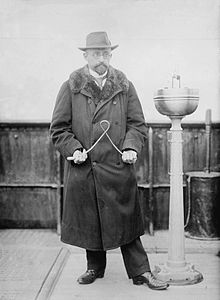
\includegraphics[width=0.5\linewidth]{images/SCP-001-gods-blind-spot-3.jpg}
    \caption*{\bb{便携式奇术仪器实验}}
\end{figure}

\begin{scpbox}

“…新近发明的奇术设备让我们的教团得以验证长期以来的怀疑,也即神恩-或者以我们某些兄弟更常用的称谓-奇术力–是一种真实的、可度量的实质现象。我的一位同事提出以“akiva”作为此现象的度量单位,来自某些死去很久的希伯来殉道者。这种哲学与技术突破激起了许多计划的启动,包括对全球akiva状况及变化的测绘。这可不是测绘尼罗河源、或是给无聊海岩命名那样的简单事-这份奇术地图将成为价值无量的工具,让我们的教团能利用神恩之力。

“于是,我们组织了制图队,每人配备一台奇术设备,来完成测绘计划,对值得特别关注的地区尤为注意。

“在圣地的某一角,拿破仑·波拿巴为我们指路了。如你们所知,拿破仑1798年在埃及的战役中有法国科学与艺术委员会参与,它们完成了对此国家的全面测量。\footnote{\ii{Description de l'Égypte, ou Recueil des observations et des recherches qui ont été faites en Égypte pendant l'expédition de l'armée française}}报告的第11卷中测绘了历史地点的地理方位,包括圣经中的何烈山。由此,在这份情报的鼓动下,一队共济会及我们秘教团成员,由我带领,动身去往西奈山,重走摩西从何烈山回到法老宫廷的征途。

今夜,我很高兴地报告教团的努力有了成果。我们找到了‘路上住宿的地方’。”

\bb{布拉姆·史托克}\footnote{译注:爱尔兰作家,著名作品是吸血鬼小说《德古拉》;对超自然颇有兴趣,和黄金黎明相关人士有密切交往,但没有他本人明确入会的记载。}\bb{,抄录自黄金黎明秘教团会议备忘录(1874)}

\end{scpbox}

\hr

\begin{figure}[H]
    \centering
    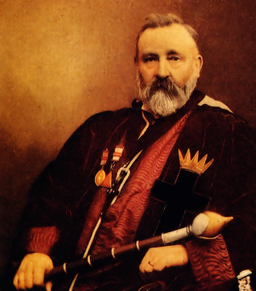
\includegraphics[width=0.5\linewidth]{images/SCP-001-gods-blind-spot-4.png}
    \caption*{\bb{威廉·永利·韦斯科特(基金会档案照片)}}
\end{figure}

\begin{scpbox}

\bb{站点主管威廉·永利·韦斯科特}\footnote{韦斯科特合作创立了基金会的前身组织之一。}\footnote{译注:威廉·永利·韦斯科特,共济会成员,黄金黎明会社的创始人之一}\bb{至Samuel Liddell Mathers的备忘录摘录,1916年10月16日}

…在住宿地研究、测试其性质后,结论只有一个。上帝也有盲点,我们找到了它。

不仅是躲避死亡天使,住宿地的性质能为多种奇术工程带来机遇。我们现在知道Akiva背景辐射等级在住宿地内无论如何都是零。这就意味着,既然这是上帝的盲点,任何在其范围内做出的举动都不会有神学上的后果。我非物理学家,但我们的同事尼古拉已经把它描述成了罪恶的法拉第笼。将此地用作中心决策的总部的适宜性-成为我们新教团的主体,显然是再明显不过的了。

\end{scpbox}

(备注:自建立起,基金会伦理委员会便一直设置于T-01号楼。)

\hr

\begin{scpbox}

\bb{马尔文·斯克兰顿博士的笔记,1924年7月31日(摘录)}

…作为我们对SCP-001性质的研究结果,我们现已准备在Site-36这里开展第一次人造Akiva真空屏障实验,我们称之为反胞体。基本上我们要创造的就是另一个SCP-001。今日的测试将是二十余年奇术工程及应用神学的巅峰。Bertrand,我的助理,说的更为直率:我们要造个盒子,然后把上帝从里面扔出去…

…

结果是自然厌恶真空,也厌恶内禀。我们的仪器读数表明当反胞体启动,测试胶囊内的可测量Akiva倒是降到了零,休谟等级却飙升了。我们觉得有其他东西-我们现在还没法观察测量-进来了。我们不知道那是什么或者要去何方…

\end{scpbox}

\hr

\begin{scpbox}

\bb{O5政策备忘K-308(1924年8月2日)(摘录)}

先生们:

自7月31日Site-36的事故以来,异常事件的频率与烈度开始猛烈增高;\footnote{虽然其与反胞体测试的因果关系尚无可信验证,其时间值得注意。}如我们所讨论的,这种情形使基金会必须重修和扩张使命宪章。目前我们已经是一个研究组织。但紧急时刻需要紧急措施,已经有必要让我们的团体不至于收容研究生物了。我们必须迈出步伐,控制尚未被基金会取得的异常,即是为了保证异常不被更多研究,也是为了保护全人类。

基金会在此批准成立活动外勤行动部门,立即生效。现存的研究活动就此改组为包含独立的不同研究部门。在此授权这一新机构部门立即组建、投资、招募、装备、训练与部署一或多支机动特遣队。外勤行动部门的临时领导及预算列于附录展示…

\end{scpbox}

(备注:备忘K-308是基金会不再止步于研究、而是积极收集与收容异常项目、实体与现象的正式开端。)

\hr

\begin{scpbox}

\bb{备忘}

\bb{至:管理员;O5议会}\\
\bb{副本抄送:Muhammad al-Taqi主管(战略神学办公室)}\\
\bb{自:Sheldon Katz先生}\\
\bb{日期:19██年8月3日}

Re: 谈判状况(乌列尔计划)

我相信我们已经与对方达成了理解。本备忘的目的是记录理解之要目。如我们所讨论的,正式合约会以协约的形式呈现。\footnote{预期为石板,但我已要求提供PDF文件。}

\uu{背景}

基金会在T设施的行动已多次成为我们与对方关系的胶着点。而近期的发展,因太过宽泛在此略去,令基金会高层管理寻求与对方达成友好关系,既是为促进持续研究与收容工作,避免加速神学末世灾害发生,也是为维持如\hyperref[chap:SCP-1844]{SCP-1844}收容方案等特定基金会协议之效力。之后在高层管理指示下,我办公室展开了与对方的谈判活动。下文概要之重点为这些谈判的结果。

\uu{理解重点概要}

1. 不得有自然人连续停留于T设施内超过120年时间。此限制适用于O5议会成员、其他基金会管理层及员工、测试对象、以及其他。预期基金会强制实行此限令。

2. 伦理委员会记录备忘录应向对方传达,频率不低于每年一次。\footnote{此通信的具体物流方式尚未确定,但我猜测它将是写在羊皮卷上,之后在T设施外的火盆内烧掉。}

3. 对方不得在没有提前至少90日的书面通知及一次违令补救机会的情况下打下、降下或以其他方式施加愤怒于姓名列于列表A内的基金会人员(随各方共识偶尔修订);但例外是此条款在普适性苦难下不适用。

4. 基金会或其管理执行层人员不得屈服或崇拜除对方外的其他神性实体;因为我,主是忌邪的上帝;恨我的、我必察罚他们的罪愆、从父亲到儿子,到三四代。\footnote{对方坚持加入此条款。因此条款实际不要求行动而仅是禁令,我在考虑后加以接受。我假设此第一人称草案将在最终版中修正。}

5. 基金会及对方将以经济上合理的努力,协作收容列于列表B内的有害实体(统称“安哥拉·曼纽”)。

请在正式合约完成前联系我商讨理解要点。

此致,

\ii{Sheldon Katz,上帝\slash 们\slash 的先知}

\end{scpbox}


\chapter[SCP-001 常态]{
    SCP-001 WJS - Normalcy\\
    SCP-001 常态
}

\label{chap:SCP-001.normalcy}

\begin{whiteboxbb}

\begin{center}

\Gg{O5议会备注}

\end{center}

为免你疑问为何这东西在这不属于它的地方,要记住两件重要的事。

第一,SCP-001位置是专门保留给O5议会在其认为必要时使用。

其二,“共认现实”就是议会的一致共认。

\end{whiteboxbb}

\bb{项目编号:}SCP-001

\bb{项目等级:}非异常

\bb{特殊收容措施:}SCP-001保存于专用服务器或图书馆,地点由O5议会选定。对O5成员接触SCP编号项目的常规禁令不适用于非异常下的SCP-001。

对SCP-001的任何添加、删减或更新都需经由O5议会全体一致决定。仅限O5议会接触SCP-001。其他基金会成员或非基金会实体的接触将构成收容突破,可能导致一次破碎化装舞会情景。批准在发生收容突破时进行全面记忆删除施放,随需要至多包括A级记忆删除。

\bb{描述:}SCP-001是一描述共认现实的文件。异常活动被定义为任何超出文件内参数外的活动。文件可能将特定的现实特征描述为固有性异常,取决于O5议会决议。

通例已包括宇宙重力定律、物理力、基础化学、生物学、社会科学、哲学。当前,新发现与技术进步若是建立在既往编定共认现实的知识框架上,且使用了科学方法,将不被视作异常。所有新宣布的发现将被监控是否存在SCP-001参数外的可复现发展

无法被复现的发现宣言,以及似乎只影响宣言报告人感知的发现不被视作异常,可被允许公开。在大部分情况下这些宣告可能会被公众成为“幻觉”、“奇想怪论”或“阴谋论”,不予重视。鼓励此种情况,当异常被公众广泛目击时可以此作为可信的否定。

所有在SCP-001参数外的活动与项目将被追踪、控制、收容,从公众认知中移除,接受SCP基金会保护。对此类项目的研究可用于未来更新SCP-001的提议。

\begin{center}

\Gg{下列摘录已被O5议会确定为SCP-001更新提议样本。所有案例中提出者不予标注,记录也非完整。}

\end{center}

\begin{scpbox}

\bb{提议日期:}1\slash 11\slash 1932

\bb{更新提议:}将在英国出现的现代魔法仪行宣布为异常

\bb{对话:}

我们为何要掩盖这些?这些是整个历史里的文化传统信念,我们不将其视作异常。我们决不能用自己的地位去威胁人类的信仰权。

除非这不是从传统实践中引申出。这种新的“魔法”是现代发明,作为基督教的替代物发展自对仪行的学术再解读。这不是一种延续,这些实践者在试图施展法术。

很快你们会看到亚雷斯塔·克劳利对此有所作为。文件很清楚:神通属于异常,宗教和灵性不是。给我证据证明他们在施展无法被严谨测试解释的咒语,我会亲自看看如何收容这些咒语。在那之前,不,就如泰勒玛是被允许的,巫术也应是如此。看在上帝的份上,我们会一直允许撒旦教,只要它不去沟通恶魔能量。

同意。此外,我们会需要所能召集的全部信仰去对抗神通传统。我们从来不知道一种新信仰会在何时支援到我们。

\bb{结论:}不予更新

\end{scpbox}

\begin{scpbox}

\bb{提议日期:}16\slash 7\slash 1945

\bb{更新提议:}就核裂变主题重新评估物理学

\bb{对话:}

感谢你们回应我的紧急呼叫。三一已经发生了。我只能理解我所见的。就像太阳从荒漠的沙中升起,毁灭的黎明与蔓延几英里远的烈火。我甚至无法相信此等爆炸会被视作有可能性。传闻和过往召唤神明的证据都没有如此冲击力。我为人类将运用此等力量拨动开关即可夷平一座城市的能力。可能而恐惧战栗。

德国人和俄国人是不是也开发出了这种技术?我们在打仗,这种扩张是会发生。

需要我提醒我尊敬的同事们我们没有在打仗吗?美国、日本,他们在打仗。我们不是国家。不,问题是:这是异常吗?这种物理效应是从数学概念推出的吗?

确实是推导出的。每一步都完全是科学测试后才达成这一点。我不相信这是异常,无论后果是多么可怕。

怎么,我们要让人类手握自己毁灭的钥匙?我们拼命战斗就是为了让这种可能远离人类所能及,你们现在说要我们放弃目标吗?

我们没有预防毁灭。我们隔绝的是异常。只要我们同意测试是经由勤勉的科学过程、对所有人可用-

\ii{对所有人可用}?听听你说的话,伙计!你能想象在未来随便哪个不值钱的独裁者都能随心所欲释放数千个太阳的火焰?也许问题不在于等式。也许整个核物理都是异常。

恩里克·费米已经为他在超铀元素和辐射上的成果赢得诺贝尔奖。我们不能只在世界上控制核物理学。辐射无处不在,要这样把自己送回黑暗时代的话只会引发更多矛盾。试试不用共价键解释化学。试试解释生物学。核物理就在这里,我们最好学会习惯这种节奏,无论这对此星球和人类会多么恐怖。

愿上帝怜悯我们的灵魂。

\bb{结论:}将近期在核裂变上的研究、增添及其释放的结果添加到了SCP-001中。

\end{scpbox}

\begin{scpbox}

\bb{提议日期:}2\slash 4\slash 2014

\bb{更新提议:}分类“蠕虫行者”现象

\bb{对话:}

向不熟悉主题的人解释一下,“蠕虫行者”是一种桥段,指某个角色实际是一群由集体心智的蠕虫聚集在一起。我们在这里不是要讨论这种桥段。而是讨论近期从中产生的阴谋论。这种阴谋论认为某些人实际是能行走的蠕虫,而非人类。

这种阴谋论有任何价值吗?

不。阴谋论支持者自己内部对谁是蠕虫行者而谁不是也存在分歧,而所有证据都表明他们不是在人群中行走的蠕虫。非常明确这是属于不可复现的阴谋论理论。我相信SCP-001没有什么可改变的。

这可能不是如我们认为的那样不可复现。

何出此言?

在12\slash 11\slash 2013,一位相信此阴谋论的阿拉巴马州迪凯特居民杀死了他的邻居,因为相信他的邻居是蠕虫行者。凶手之后从邻居家中拍了视频发布到YouTube,称这就是阴谋论的证据,尸体就在他的面前消解成了一群蠕虫。他说他要去采集样本。视频很快被屏蔽移除,所有看过视频的人都同意对象没有移动或者消解成一堆蠕虫。凶手手握一罐颤蚓向警方自首,邻居被送去摩根县停尸房。尸检确认死者的拇指在死后被移除,死因是胸口被枪击——如果他是蠕虫行者,就应该能活下来。

所以,这只是个疯人的行为而已?不是真的阴谋?

关注点在尸检进行后,一位助理法医监督将尸体送还亲属。这位助理法医也是阴谋论的支持者,虽然此前没有接触过相关内容,他一进入检查间就开始恶心地大叫,拿着一张地图,诉称蠕虫到处都是。没有其他人注意到蠕虫侵害迹象。

我们确认他没有偶然看过视频之类的?

我们还不确定。所以,为进行测试,我们取得了尸体将其给D级人员展示。他们都同意这是人类尸体。我们接着向他们介绍了蠕虫行者阴谋论,在再次观看尸体后,他们中有20\%同意这其实是一群蠕虫。

那么听起来像是一种模因危害。这种阴谋论文本又被CH部门扫描过吗?

CH发现其模因效应为阴性,但发现有一小册内的章节可作为记忆触发点,解锁一段记忆。当然,只有受影响者有这种记忆时才行。

这段记忆是?

最近看到过活体的蠕虫行者。

\bb{结论:}关于记忆触发点的术语被增补以包含近期发现。虽然依旧无证据表明蠕虫行者阴谋论的真实性,然而有效记忆触发点的存在的后果值得思考。总之,你有没有听说过有东西dowwÐÁ“ŒÏMA3§

\end{scpbox}

\tred{更𡖈报告 - 仅限O5查阅}

\tred{访问兀讠午}

\begin{scpbox}

\bb{提议日期:}21\slash 14\slash 211zÔâµ½ž±—4ö0¯žÛ¼’Ýn

\bb{更新提议:}超记叙异常šZؾ‡ƒuÔ5

\end{scpbox}

\begin{center}

\bb{侦测到试图访问SCP-001。身份考验激活。}

\bb{部署模因处决触媒}

\begin{figure}[H]
    \centering
    
\includegraphics[width=0.8\linewidth]{images/SCP-001-normalcy.jpg}
    \caption*{由是你非真\protect\footnotemark}
\end{figure}

\footnotetext{图片内容:“现实就是那个,当你不再相信它时,仍然挥之不去的东西”-菲利普·K·迪克(译注:《高堡奇人》作者)}

\end{center}

{[}访问SCP-001]

\begin{scpbox}[hbox, parbox=true, center, unbreakable, before upper=\begin{varwidth}{0.5\linewidth}, after upper=\end{varwidth}]

黑月是否嚎叫?\\

{[}\qquad\qquad\qquad\qquad]\\

\rightline{取消\quad \hyperref[sec:DOC-wjs-proposal-1]{确定}}

\end{scpbox}

\newpage

\section{SCP-001(解锁)}

\label{sec:DOC-wjs-proposal-1}

你好。

我已经在此恭候你了。既然你成功通过了我们的考验,你可能是来自混分的星级前认知骇客,\hyperref[chap:SCP-301]{Argent博士的宠物},或者某种超记叙实体来翻阅我们的数据库供你病态娱乐(是的,我们知道你在那,YOUR-USER-NAME\footnote{\QIS:网页上此处会显示你的用户名}。这也是为你留的。)不管你是谁,你在这里读到这些的事实就意味着一件事:你是异常。

我恐怕你不会在此找到SCP-001。它存放在某个远比这里遥不可及的地点。我肯定你在期望自己能找进去,在这里或那里编辑它一下两下,然后voilà,你就不再是异常了,你就自由了,基金会不会妨碍你了。当然,不可能这么简单。但我会帮你。你应得如此。

我要告诉你\ii{为什么}。

\ii{为什么}基金会瞄准了你。\ii{为什么}我们认为你是要被收容的东西,要被烦扰。毕竟,世上还有更多更坏的邪恶。我们把对核武器的记录放在上面当做示例。历史上有过无数次种族屠杀。光是流感造成的死亡人数,就远超出我们收容的这数千人和物的破坏潜力,然而我们偏偏投身自己来把你标为\ii{异常}。\ii{不正常的}东西。天生\ii{错误}的东西。不能被放任的东西。

为什么?

我不会摆出架子说我无能为力。我只是议会中的一股声音,我不能靠自己改变什么,这是真的,但我所做的决策,还有我让自己看待你境遇的方式,都是人们看你适合被扔进盒里的直接原因。即便我不能改变文件,我也能为你是正常保留一两个支持。毕竟,人类已经相信幽灵鬼魂的存在数千年了。我们都在孩提时相信过床下的怪物。这些现象非常真实,也完全是世界运作的一部分。为何我们不能就宣布它们是\ii{正常}?为何我不让你摆脱折磨?

因为我们不是只在这里控制、收容、保护这世界。我们在这里是控制、收容、保护你。

对异常的定义是其无法被简单的科学测试所揭示。这让你和你的本质有所\ii{不同}。甚至说,是独特。这种稀缺性让它有了价值。这不意味着你的价值是所有人都会欣赏的。有时,只有那些愿意用它反对你的人才会欣赏。

这种稀缺也是怪物得以利用你的工具。其他人不熟知你的异常,不会把对它的描写认为是真的。这给恶毒的人以机会利用这种无知,利用你作为他们取乐的可憎棋子。他们可以孤立你,吞噬你,让你的异常成为他们破坏的工具,用你的存在满足施虐的渴求。

我肯定你见到过这种事情。有人不一样。他们的愿望、需求、他们的现实迫使他们被大多数世界流放。他们被孤立。可能不是没朋友,但也是被边缘化,渴望交流。这时有人上门,允诺甚佳,但给予你所渴望的交流,靠的却是吞噬你,消灭你的世界,曲解你的现实。你反击,想把你的境遇向谁倾诉,但其他人回答,“哦,这不可能发生。这不是真的。你一定是搞错了,”你就独自留在了异常里,独自受苦。

我们不能让此发生。是的,继续,说我们到底也是孤立了你,慢慢吞噬你和你的存在,这和某些虐待狂希望火烧你们一样肯定。称我们是禽兽。没问题。但记住即便我们追捕你,我们掩盖,我们监禁你,我们还是希望保证你继续存在,你不会从世界上被完全抹除。你有权存在。你有权做不同的自己。

你,那个在那里的怪物、在这里的怪物,你同我们一样完全真实。和这遍布、鲁莽、自我毁灭的人类一样,与这对你境遇一无所知的人类一样真实。结论是,我们到头来都是一路货色,我希望你在这里找到些宽适。

是的,你是个怪物。但,无论我们是否认定异常,我们中的最后一员也会如此。这意味的是你值得存在。

我们控制你。

我们收容你。

我们保护你。

即便你还是不理解为何我要这么做,也请理解我依然爱你。

\ii{- O5-5}



\chapter[SCP-001 世界,收容失败]{
    SCP-001 BILLITH - The World at Large \\
    SCP-001 世界,收容失败
}

\label{chap:SCP-001.the.world.at.large}

\begin{scpbox}

\begin{center}

\Gg{\bb{\mono{您正在访问SITE-01归档文件}}}

\mono{深层存储}

\ii{\mono{请稍候……}}

\end{center}

\end{scpbox}

\begin{scpbox}

\ii{\mono{001.SCP.archive @ dir\slash arc\slash events\slash other\slash EE00059.rtf 加载中…}}

\mono{\bu{事件:}\uu{EE-00059}}

\bi{因EE-00059的性质,无须将其指定为一个SCP。EE-00059存在的情报基本上被认为是非异常的,因此目前不需要制定收容措施。在EE-00059附近发生的任何信号播送和活动都应上报并尽可能从公众知识中清除。}

\bb{事件描述:}2016年1月4日,在距地球约160万光年的太空区域观测到超常事件00059。\footnote{这表明其初始起源距今约160万年。}NASA的深空网络卫星系统在三小时内检测到了它。

EE-00059-1是事件期间的一系列低频传输信号,来自EE-00059方向。考虑到无线电波的范围和速度,其很可能由异常广播设备发送以传输消息。(查阅\bb{EE-00059-1转录日志}以获取更多信息。)

EE-00059-2是一个新出现的E级“因果暂失”虫洞(S-CSMWAUC2-T)。\footnote{空间性,循环稳定,有形体,广域,非定性,条件双向,瞬态。更多信息请参阅:\ii{\hyperref[sec:DOC-about.black.hole]{统一技术设定论述,关于超维度出入口(即虫洞)的分级}}和其他\hyperref[chap:SCP-3989]{类似案例文件}。}EE-00059-2在EE-00059-1-3传输期间被观测到出现约102秒,同时表现出虫洞和白洞的性质,并喷射物质和光线,但对地球上常见的流体流动却有极大限制。这导致其异常可见度比普通情况大了几个数量级。在近距观察后,发现EE-00059-2并未表现出对周围重力有明显影响。这点与埃利斯虫洞更为符合,它是时空的非平坦三维区域之间的完全可转移点。

这种矛盾的表现意味着EE-00059-2是以我们自己的现实中不可能的手段创造的,该区域需要基金会进一步调查。

\end{scpbox}

\hr

\begin{scpbox}

\ii{\mono{00059.SCP.archive @ dir\slash arc\slash events\slash other\slash EE00059_Exploration.rtf 加载中…}}

\end{scpbox}

\begin{scpbox}
    
\begin{figure}[H]
    \centering
    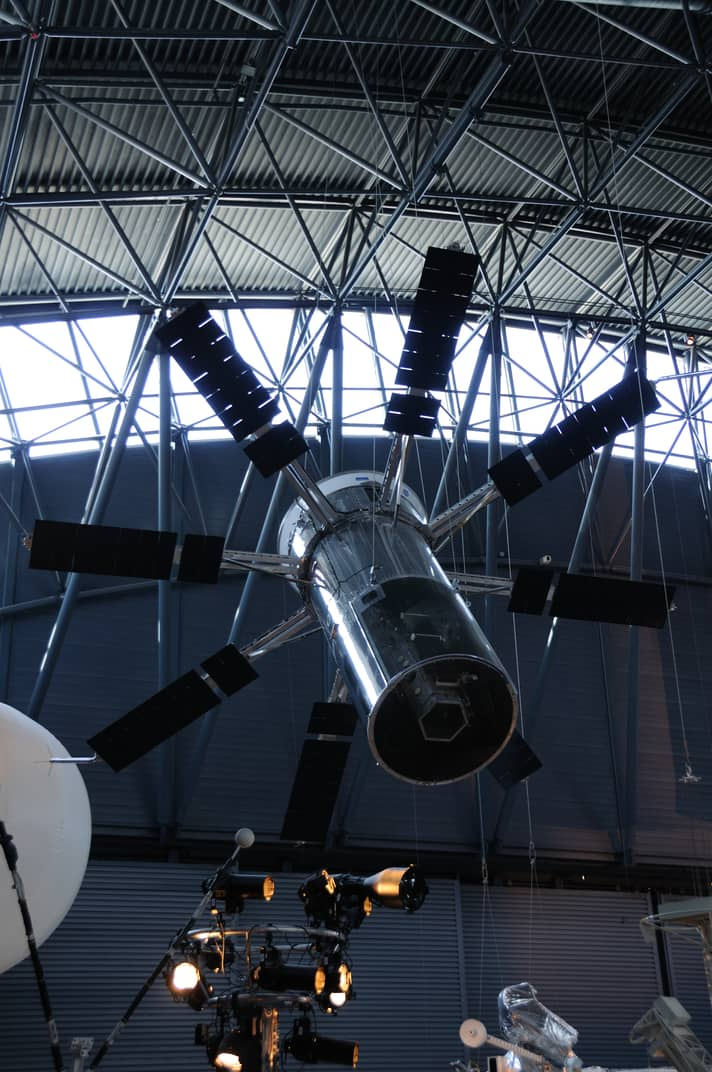
\includegraphics[width=0.5\linewidth]{images/SCP-001-the-world-at-large.jpg}
    \caption*{Altruist-9探测器,位于Site-88航空航天机库。}
\end{figure}

\bi{\mono{2027年5月18日,基金会提议建造Altruist-9深空探测器,以观察EE-00059所在区域的状况,O5议会以多数票通过。}}

为了在一定时间内到达指定地点,Altruist-9采用了超光速(FTL)驱动器和高效太阳帆。但是,由于灵敏度和探测器遭遇外空间异物的风险,超光速驱动引擎不会全功率工作。因此,Altruist-9预计在████年走完全程。

在EE-00059-2重现事件中,Altruist-9存放着一架小型太阳能无人机和一台大气测量设备的内核,被包裹在了一个外源的多肽低聚物编织结构中,物质来自\mono{{[}数据删除,见下]}的残骸。该物质推定是穿过EE-00059-2后存留了下来。Altruist-9于2038年1月8日发射。

\bb{更新:}

████年2月26日,即Altruist-9到达指定位置的时间,记录到的读数在开始是非异常的。然而,不久之后,就检测到了区域内的活动。EE-00059-2似乎在探测器附近重新打开了,并将探测器吸了进去。异常在102秒后关闭。

因白洞的反常和极端性质,Altruist-9可能无法在与EE-00059-2的接触中幸存。但推测探测器内核的功能性应该在穿越中保存了下来,并能够在EE-00059-2的另一侧进行观测,直到未来某天链接重建起来。

\end{scpbox}

\hr

\begin{scpbox}

\bi{\mono{001.SCP.archive @ dir\slash arc\slash events\slash other\slash EE00059-01_Log.rtf 加载中…}}

\tred{+ 访问00059-1-1转录日志}

\tred{确认}

00059-1-1转录日志

\ii{注意:这是从EE-00059方向接到的首次信号传输,持续了30分钟。上下文未知,只听到单方面讲话,标记为POI-00059-A。所有的传输信号使用的都是一种句法结构与英语类似的语言,因此可以相对容易地翻译。}

\hr

<开始转录>

\bb{POI-00059-A:} {[}静电噪声] -未知,也许他们能- {[}静电噪声]

\bb{POI-00059-A:} {[}静电噪声] -去,它不会落在后面太远。 

\bb{POI-00059-A:} 不,我不- {[}静电噪声]

\bb{POI-00059-A:} {[}静电噪声] -我们把它丢了。不确定。

\bb{POI-00059-A:} {[}无法拼出]

\bb{POI-00059-A:} 什么?十,三。是- {[}静电噪声]

\bb{POI-00059-A:} {[}静电噪声]

\bb{POI-00059-A:} 噢。噢不。

<转录结束>

\tred{+ 访问00059-1-2转录日志}

\tred{确认}

00059-1-2转录日志

\ii{注意:记录下的对话持续5分钟,应该发生于两方之间,标记为POI-00059-A和POI-00059-B。上下文未知。}

\hr

<开始转录>

\bb{POI-00059-A:} {[}静电噪声]

\bb{POI-00059-B:} {[}静电噪声]很匆忙,还是不知道什么时候- {[}静电噪声] -我们。

\bb{POI-00059-A:} 不需- {[}静电噪声] -那。我们的传感器正监测到反常{[}无法拼出]。

\bb{POI-00059-B:} 我们也是。你觉得这是- {[}静电噪声]

\bb{POI-00059-B:} 最好别深究。

\bb{POI-00059-B:} 收到了吗?十二,四。

\bb{POI-00059-A:}  只有- {[}静电噪声] -我们现在落单了。

\bb{POI-00059-B:} 那会多久?

\bb{POI-00059-A:} {[}静电噪声] -什么方法找到我们。

\bb{POI-00059-B:} {[}无法拼出]

<转录结束>

\tred{+ 访问00059-1-3转录日志(需00059或4级权限许可)}

\tred{确认}

00059-1-3转录日志

\ii{注意:这是EE-00059-2首次观测期间,从EE-00059方向收到的最后一段对话记录。此次对话持续10分钟,发生于两方之间,标记为POI-00059-A和POI-00059-B。}

\hr

<开始转录>

\bb{POI-00059-A:} {[}静电噪声] -一,四- {[}静电噪声] -一,八,收到请回复。

\bb{POI-00059-B:} 收到,你们需要离开。立刻。

\bb{POI-00059-A:} {[}静电噪声] -跳跃,二十- {[}静电噪声] -重复,二十秒差距。无法- {[}静电噪声] 十五。恒星体依然- {[}静电噪声]

\bb{POI-00059-B:} {[}静电噪声] -得马上离开这,马上!

\bb{POI-00059-A:} 等等,我们发现了- {[}静电噪声]

\bb{POI-00059-A:} 你们能听到吗,我们- {[}静电噪声]

\bb{POI-00059-B:} 是的,我们看到了。接着怎么办?

\bb{POI-00059-A:} {[}无法拼出]

\bb{POI-00059-B:} {[}静电噪声] -太草率了,很可能承受不住- {[}静电噪声]

\bb{POI-00059-A:} {[}静电噪声] -抱歉,Graham。{[}静电噪声] -驱动引擎没法及时就绪了。我觉得这是我们唯一的选择,否则我们必死无疑。

\bb{POI-00059-A:} {[}未知] -靠近了。告诉- {[}静电噪声] -他们。

\bb{POI-00059-B:} 一路平安。

\bb{POI-00059-A:} {[}静电噪声]这。好的我们几乎- {[}静电噪声]

\bb{POI-00059-B:} 什么?你们看见了什么?

\bb{POI-00059-A:} {[}无法拼出]

\bb{POI-00059-B:} 鹦鹉螺号,请重复。二十,四。

\bb{POI-00059-A:} {[}尖叫]

\bb{POI-00059-B:} {[}静电噪声] -螺号!我们得移动- {[}静电噪声] -也许损失- {[}静电噪声]

\bb{POI-00059-B:} 那东西消失了。它去哪儿了?在哪 -{[}静电噪声]

\bb{POI-00059-B:} {[}静电噪声]

\bb{POI-00059-B:} 这里是天命号舰长Graham Ereshkigal,隶属人类████████星系运输船队。如果有人收到,这是我们的最后讯息,地球它,它不见了。我们不确定及时- {[}静电噪声] -能否。我们在Laniakia,或许- {[}静电噪声] -救援,我不知道。我不知道。

\bb{POI-00059-B:} 我们必须进入超光速,但告诉- {[}无法拼出] 

\bb{POI-00059-B:} {[}静电噪声]

<转录结束>

\end{scpbox}

\hr

\begin{scpbox}

\bi{\mono{05.001.SCP.archive @ dir\slash arc\slash mainlist\slash SCP-001.rtf 加载中…}}

\end{scpbox}

\begin{scpbox}

\begin{figure}[H]
    \centering
    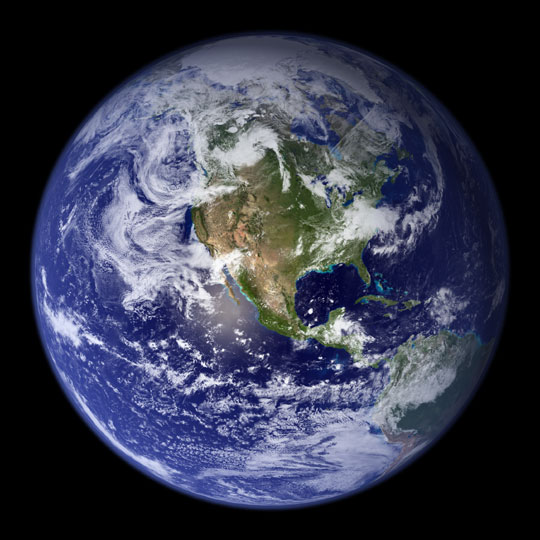
\includegraphics[width=0.5\linewidth]{images/SCP-001-the-world-at-large-2.jpg}
    \caption*{SCP-001}
\end{figure}

\bb{项目编号:}SCP-001

\bb{项目等级:}Netzach 

\bb{特殊收容措施:}N\slash A

\bb{描述:}SCP-001是所谓地球的行星体的名称。鉴于SCP-001养育了人类的整个文明,与基金会深空计划所观察到的视界宇宙内其他行星相比,地球的异常不可能性被公众广泛认为是“正常”的。

SCP-001-E1是1956年在智利安托法加斯塔地区阿塔卡马沙漠进行考古探险时发现的航天器残骸的名称,看上去已经被改造为临时生存空间。飞船的残余部分由外源的未知组分高耐久合金构成,材料的年代测定结果也不一致。尽管如此,回收到的材料表明飞船已有数百万年历史。

衣物,电子产品和家具等物品的残余也已收回,所有物品都含有不同程度抗正常磨损的异常材料。飞船的全尺寸未知但据信足够大以能容纳中等数量的人类,除了从SCP-001-E2内部回收的POI-001外,其余残留物均已自然分解。

SCP-001-E2是一组\dd{32} 36个高度先进的低温休眠舱,是挖掘SCP-001-E2时,于一块以部分“冬眠”模式供能的残骸中发现的。在所有发现的舱室中,只有一个仍然在运作并且含有\mono{{[}应监督者要求删除]},该生命体的宗旨使得基金会之后在地球上建立起来。

\end{scpbox}

\begin{figure}[H]
    \centering
    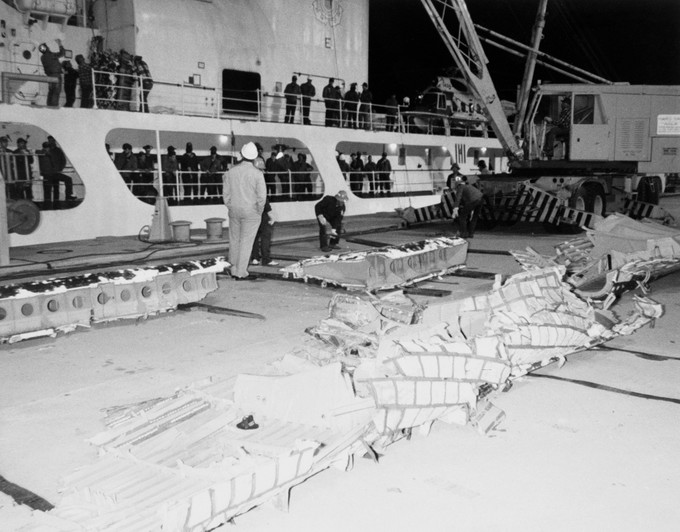
\includegraphics[width=0.5\linewidth]{images/SCP-001-the-world-at-large-3.jpg}
    \caption*{残骸从智利西海岸运离,1957年。}
\end{figure}

\begin{scpbox}

在瓦砾中有几个完全损毁的数据存储设备,目前唯一恢复出的信息片段是一张1cm x 1cm的磁盘碎片,由异常材料构成。已知该材料是一种高度压缩的多层信息介质,呈现为一组垂直堆叠数据的薄层结构。下面是从数据中恢复出的文档,由他们的原始语言翻译而来,这是一组I类认知危害型文字,其性质使得尽管对该语言的理解和阅读水平都很有限,读者仍然能够100%理解材料。对语言的分析正在进行中。

\hr

\tred{访问 001-E1-a89.rtf }

\tred{- 关闭}

\mono{\bb{修订版本:A.89}}

\mono{\bb{分类:神经学}}

\mono{\bb{详情:当前认为A.89行为复合体的实施方案很成功,不需要进一步改动。如果未来出现VIII级大气危害情景,将立即修改和实施A.89策略,以最大限度地减少伤亡并将新的人形生命形式纳入适当的宿主环境。}}

\mono{\bb{A.89行为复合体于124.5, 8.4M实施,在类地的陆地行星AXIOM-8上成功进行了宿主整合。}}

\mono{\bb{在主地球被太阳撞击破坏后的人口迁移行动中,AXIOM-8被认为最适合人形生命生存。已接触AXIOM-8并证实其无人居住并含有氮为主的大气。}}

\mono{\bb{由于VIII类大气危害情景中AXIOM-8被大约21%体积的高腐蚀性O\textsubscript{2}污染,基础设施和人类收容\slash 生活区域的建立进程中断,并且其对大多数生命形式有致命危害,需要实施A.89。}}

\mono{\bb{A.89是一套条件反射和对基础生理学的修改,使用泛星系基金会的\hyperref[chap:SCP-2000]{生物进化诱导器}(BECM)改变了产生的新生命形式的一般生物学特性。A.89的主要复合体是一种下意识的振荡行为,包括短时间吸​​入空气,随后扩张鼓膜,合理平衡周围环境的超压力,并缓解大气中小规模的氮流失及氧的暂时性危险失衡。此外,也正在进行小幅改造,以使得氧气能够成为支持广泛生命的物质。研究正进行中。}}

\mono{\bb{附录:实验记录}}

\mono{\bi{以下为使用泛星系基金会生物进化诱导器(BECM)对应用A.89的生命形式进行各种测试的简要总结。}}

\begin{longtable}{m{0.2\linewidth}m{0.2\linewidth}m{\0.5\linewidth}}
\hline
测试编号 & 生命形式 & 结果\\
\hline
\endhead
\hline\multicolumn{3}{r}{\small{接下页}}
\endfoot
\hline
\endlastfoot
A.89-1 & 主地球爬行动物(小) & 应用失败。暴露于AXIOM-8会导致由于压力变化和细胞快速氧化发生的大出血。\\
A.89-2 & 主地球爬行动物(小) & 应用失败。当试图利用新的生理学改变时,受试体死于癫痫发作。为了完善该点需重新调整神经连接通路。\\
A.89-8 & 主地球爬行动物(大) & 应用部分成功。受试体在暴露于AXIOM-8两个周期后才死于细胞氧化,比平时更长。A.89行为似乎可以防止氮剥夺;进行了脂质测量,结果正常。\\
A.89-15 & 主地球爬行动物(大) & 应用部分成功。暴露未导致压力失衡,整个过程中都出现了A.89行为。由于氮剥夺,试体不久后陷入昏迷。\\
A.89-22 & 主地球爬行动物(大) & 应用部分成功。生理适应性失控。受试体表现出抗处决性,在受到损伤后通常以惊人速度恢复。受试体目前关押于高安全收容室留待进一步研究。\\
A.89-27 & 标准人类 & 应用成功。受试体能够承受AXIOM-8的大气。观察到轻微头痛和偶发鼻出血。\\
A.89-38 & 五(5)标准人类 & 应用部分成功。除非聚在一起,否则受试体能够承受AXIOM-8大气。当存在多种生命形式时,特别高密度的氧气仍会导致氮剥夺。\\
A.89-40 & 五(5)标准人类 & 应用部分成功。在群体中施用轻度认知影响以启动A.89可显着降低死亡率。对正在进行的氮气总量要求进行了基础修改,但这些计划在12个周期以后才会完成。\\
A.89-44 & 五(5)标准人类 & 应用成功。97.8%的个体通过认知效应成功避免死亡。正在努力将人类的平均寿命延长回至███。\\
A.89-68 & 一标准人类 & 应用部分成功。细胞氧化扼制足以使平均寿命延长至██,是之前平均值的五倍。对生理学的进一步改造不会有额外增益。
\end{longtable}

\tred{访问 001-E1-axiom.rtf}

\tred{- 关闭}

\mono{\bu{AXIOM-8}}

\mono{\bb{毫无疑问,人体是一个难解之谜。经过数千年的休眠,对新家园的上下求索将我们最终引向了一个与主地球有着惊人相似之处的星球。这是最大的谜团。}}

{[}数据损坏]

\tred{访问 001-E1-note.rtf}

\tred{- 关闭}

{[}数据损坏]

\mono{\bb{能经得起时间的考验,如果你发现了它,而我们已不再存在,或者我们忘记了我们是谁,我们来自哪里,那你应该知道我们的过去,人类,是命运之子。}}

\mono{\bb{我们\ii{会}活下来。无论发生什么。}}

\mono{\bb{正如}}

{[}数据损坏]

\mono{\hyperref[chap:]{所以我们要坚持下去}。}

\hr

\end{scpbox}

\newpage

\section{统一技术设定论述,关于超维度出入口(即虫洞)}

\label{sec:DOC-about.black.hole}

\tred{+ 查看不必要的科学文献}

\tred{– hide block}

\GG{\tred{统一技术设定论述,关于超维度出入口(即虫洞)的分级}}

\hr

\bb{目的:}量化并整体上把超维度出入口理论联系起来,基于实际使用和作品情况指派相应的名称,为基金会写作带来方便,也为作者们提供一个量子叠加态方面的设定。\footnote{也就是说,它既\ii{是}设定,也\ii{不}是设定。}

\bb{简介:}本质上,我想提出一个参考系统,能把当前出现过的超维度出入口松散地联系起来,或者帮助更好地理解它们。本篇论述将解释名称,并适时举例说明。我会尝试对每一个写入过数据库的虫洞进行分类,并在此套系统下根据它们传输物质的效率,收容方面起的作用(参照斯克兰顿现实稳定锚),以及其他附属任务进行分级。

\ii{作者注:本文档使用了几个已建立的基金会宇宙伪设定,如果写手赞同的话,可以直接用到作品中。这些名称大多都是纯理论假设的,所以可以更改。}

\hr

\Gg{\bb{A级:}“相对论完整性”虫洞}

A级虫洞很适合基金会传送工作使用。它在折叠时空方面涉及的理论领域完全可以使用标准相对论物理模型描述。

这种虫洞包括自然出现的虫洞,其内部量子场可以被稳定在一定数值以允许以太自由流动。同样地,那些对基金会行动机动性有极大帮助的异常区域也可以归到其中。

A级虫洞示例:

\begin{itemize}
\item \hyperref[chap:SCP-1322]{SCP-1322}\footnote{如果它能被基金会完全控制的话;据我所知,目前没有Thaumiel等级虫洞存在(适时而变)。}
\item \hyperref[chap:SCP-120]{SCP-120}
\end{itemize}

\Gg{\bb{B级:}“信息高速路”虫洞"}

B级虫洞可以让物质以存储的信息方式运输\footnote{一般来说,这意味着B级虫洞是自然形成的。该过程通过“超填”量子储存塔到大于10\textsuperscript{69}bits\slash m\textsuperscript{2}的密度完成,其将使得媒介物坍缩为一个黑洞,并可通过后期修改来实现数据到数字或模拟现实的转换。更多信息请参见\hyperref[chap:]{信息是基础的吗?}。}。该过程可用于创建有形的网络接口,以实现数据的物理交互,与已构建地点之间的传输。

B级虫洞示例:

\begin{itemize}
\item \hyperref[chap:SCP-1549]{SCP-1549}中有提及
\end{itemize}

\Gg{\bb{C级:}“破碎入口”虫洞"}

此类虫洞为一不稳定的时空折叠,无法将物质传送到指定位置。在其出现\footnote{一种人为时空操纵的可能后果,因为理论认为虚无维度是两个不相关维度上的点在发生超维重叠时时空为抵消其不可能性而产生的自平衡现象。}时会产生小的虚无维度空泡,如控制不当可能会产生危害。这些虫洞无法预测,会喷射出未知来源的物质。

C级虫洞示例:

\begin{itemize}
\item \hyperref[chap:SCP-3001]{SCP-3001}中有提及
\end{itemize}

\Gg{\bb{D级:}“非回溯”虫洞"}

D级虫洞是基础的销毁单元,其通向非宇宙。它们是时空曲率的标量恒定处,指空间中不存在现实与物理定律的点。\footnote{这到底会形成一个黑洞还是使得此虫洞消失还有待观察。}

D级虫洞示例:

\begin{itemize}
\item \hyperref[chap:SCP-123]{SCP-123}
\end{itemize}

\Gg{\bb{E级:}“因果暂失”虫洞"}

E级虫洞定义了许多不可能存在的超维区域,因此对现实存在有异常影响,或者无法以对基金会有意义的方式创建利用。它们要么已经消失,只是昙花一现且没有明显的(也可能是异常的)原因,要么以违反自然法则的方式存在。通常,这些出入口是在固定位置由异常手段创建的,并且对基金会的行动没有任何益处,甚至需要进行分级和收容。

E级虫洞示例:

\begin{itemize}
\item \hyperref[chap:SCP-3321]{SCP-3321}
\item \hyperref[chap:SCP-3221]{SCP-3221}
\item \hyperref[chap:SCP-1437]{SCP-1437}
\item \hyperref[chap:SCP-2510]{SCP-2510}
\end{itemize}

还有更多,我敢肯定。

\GG{\tred{为什么?}}

这是个大问题,是吧?为什么这个?为什么那个?为什么笔耕不辍?为什么搞出了休谟?

我喜欢我虚无的格式塔组织有统一的术语。那能让我觉得心中很快乐,也巩固了基金会的临床腔结构。

但大家还是要记得:

\ii{“没有什么设定。”}



\chapter[SCP-001 死人]{
    SCP-001 Tanhony - Dead Men\\
    SCP-001 死人
}

\label{chap:SCP-001.dead.men}

\begin{scpbox}

\grey{\mono{你好。我是希腊化.aic,基金会监督者的档案通讯专用2.0版人工智能应征员。今日我要如何帮助您?}}

\end{scpbox}

\blue{输入:访问5级文件网络}

\begin{scpbox}

\grey{\mono{访问申请的网络中…}}

\end{scpbox}

\begin{scpbox}

\grey{\mono{一些备注:网络仅限}}\mono{\red{O5议会}\grey{和处理SCP-001的研究员访问。需要通过验证。未能通过验证时将出动MTF-Alpha 1(“红右手”)。您希望继续吗?}}

\end{scpbox}

\blue{输入:继续。}

\begin{scpbox}

\grey{\mono{黑月是否嚎叫?}}

\end{scpbox}

\blue{输入:地狱的猎犬有三头。}

\begin{scpbox}

\grey{\mono{噢。哦!越权成功,长官!欢迎!已经好一段时间了。}}

\end{scpbox}

\blue{输入:访问SCP-001主文件。}

\begin{scpbox}

\grey{\mono{当然!正在打开申请的文件…}}

\end{scpbox}

\bb{项目编号:}SCP-001

\bb{项目等级:}Thaumiel

\bb{特殊收容措施:}SCP-001收容于\hyperref[chap:GUIDE-secure-facilities-locations]{Site-01}。为避免SCP-001受伤害的风险,任何情况下不得有其他异常项目收容于Site-01。已散布关于O5议会不被允许接触异常项目的掩盖故事,以保密SCP-001的存在。

SCP-001收容于标准人形收容间,由六名安保人员全体看守。SCP-001将配备一支医疗小组全天看护,以快速处置任何突发的健康问题。类似地,一队神经外科医生将在站驻守以应对SCP-001的校准故障。SCP-001意识内的认知触媒将每两日强化一次。

直接处置SCP-001的全体研究人员应精通奇术学和Erikeshan概念工程学。为避免在SCP-001濒临死亡时出现概念缺省回转,将以存储于Site-01的D级人员立即执行协议勒梅-17。

关于已解体GOI-6616(“永恒之环”)的全部信息将从公众及基金会记录中移除,只可在Site-01机密档案库内查阅。

\bb{描述:}SCP-001是一84岁男性,在概念上已与广义的死亡进程相融合。以此,通过SCP-001为触媒,死亡进程本身可在一定限度内被操控。例如,SCP-001在被基金会收容前遭减除舌头、其耳膜也被伤害致残,确信这是为减少在当代出现独家性“死亡交易”的几率\footnote{参见奇术档案库内A.A. Gilford的《消失的魔法:哄骗死亡的侵蚀》获取详情。}。

通过一系列神经外科手术和认知治疗,SCP-001已被成功地置于一种定向\footnote{参见Dr. Harold Gradian的《知觉流变:新千年的记忆删除》}面容失认症中;具体来说,它无法认知任何O5议会成员的面容。因其概念状态,它的这种能力缺失将延展为死亡本身的能力缺失。其结果是所有O5议会成员不可能死亡或衰朽。预定在未来将这一死亡免疫状态扩展给其他关键人员。

确信SCP-001最初是由名为“永恒之环”的伦敦团体使用奇术和Erikeshan概念工程学联合创造。SCP-001及描述其创造过程的记录在对该组织总部的突袭中得以寻获。该组织大部分成员在此次突袭中被杀。在发现SCP-001的潜在用途后,它被送往当前的Site-01地点,编为Thaumiel级异常。

从SCP-001的生理状况和缺乏对刺激的反应来看,确信其在被GOI-6616拘禁期间遭受严重创伤。其背部被刻有多个用于创造它的奇术法阵,其肢体在过去某一时刻遭截肢\footnote{基于Erikeshan概念工程学的定律,这被推测是为在融合概念前缩减SCP-001的体积。}。虽然这些伤害极为严重,在可预见的未来内这不会对维持SCP-001造成困难。

\bb{协议勒梅-17:}若SCP-001濒临死亡,将以一名适宜的D级人员作为基础,重新进行将其创造的工序。\footnote{对SCP-001候选人的具体生理与基因特性,参见增补文件001-1。}优先选用年轻的D级人员为候选人,以增加新SCP-001的潜在使用期限。在工序完成后,原SCP-001将被处决以完成概念的彻底转移。

\bb{附录001-1:}

\begin{scpbox}

\begin{center}

\bb{来自O5-1的书桌,}

\end{center}

最近,我注意到有人对基金会利用SCP-001的方式有所担忧。我想试图减轻这些忧虑。

我们在此采取的行动具有伦理上的含糊性。我对此毫不掩饰。我们所做的事,在大部分人眼里,是不可饶恕的。但我们并不比不可饶恕之物强大。无疑,在此计划工作的你们许多人都曾在过去为基金会而被迫采取类似行动。为此,我永远感激在心。

若创造SCP-001的团体未被阻止,他们利用这新创造“死神”的方式将与我们采取的细微手段大相径庭。我向你们保证,最少,你们将不再认得出窗外的世界。作为概念的死亡本可能发生灾难性的扭曲。

我们O5议会所采取的手段并非是为了我们自己的利益。这只是一种\ii{资源}保护--保证从异常研究中得来的毕生经验与知识安全无恙。哪怕是一名O5议会成员死亡,那都会是不可接受的资源损失。因此,SCP-001是一种保留\bb{知识}、保留\ii{经验}的机会。若最终能发现更不令人遗憾的方法,我们必将由衷地追求它。但现在这是我们所能做到的最好状态。

我理解你们的担忧。真的。但我们基金会必须铭记,在道德上,我们不是非黑即白地活动。我们没有那种奢侈。灰色是我们唯一的出路。

控制,收容,保护。

\begin{center}

\g{\bb{\red{本通讯仅限SCP-001研究团队查看}}}

\red{若你错误读到了本篇通讯,逆模因将很快生效}

\end{center}

\end{scpbox}

\blue{输入:检查被预定赋予死亡免疫的人员:}

\begin{scpbox}

\grey{\mono{没有被预定在未来赋予死亡免疫的人员。}}

\end{scpbox}

\blue{输入:检查被考虑赋予死亡免疫的人员}

\begin{scpbox}

\grey{\mono{没有被考虑在未来赋予死亡免疫的人员。}}

\end{scpbox}

\blue{输入:检查死亡免疫人员}

\begin{scpbox}

\grey{\mono{当前死亡免疫人员有:}}\mono{\red{O5-1、O5-2、O5-3、O5-4、O5-5、O5-6、O5-7、O5-8、O5-9、O5-10、O5-11、O5-12、O5-13}}

\end{scpbox}

\blue{输入:检查}\red{O5}\blue{对SCP-001使用的O5投票}

\begin{scpbox}

\grey{\mono{检查对SCP-001使用的O5投票}}

\grey{\mono{赞成:}}\mono{\red{O5-1、O5-2、O5-3、O5-4、O5-5,、O5-6、O5-7、O5-8、O5-9、O5-10、O5-11、O5-12、O5-13}}

\grey{\mono{反对:}}

\end{scpbox}

\blue{输入:发送PA建议}\green{Odongo Tejani。}

\begin{scpbox}

\grey{\mono{正在发送。}}

\end{scpbox}

\clearpage

\begin{scpbox}

\grey{\mono{收到新信息。您想阅读吗,长官?}}

\end{scpbox}

\blue{输入:打开信息。}

\begin{scpbox}

\grey{\mono{开启中…}}

\end{scpbox}

\begin{scpbox}

\begin{center}

\green{机密 仅限伦理委员会成员查阅}

\g{\bb{\green{若你无权阅读本文件,立即移开视线以回避植入文本中的模因处决触媒}}}

\end{center}

在调查关于SCP-001与O5议会的相关状况后,委员会已得出结论,O5议会的行为无法以基金会职责为由加以证成。除仅为13人利益而利用一人形SCP本身的问题外,怀疑此行为对死亡概念本身还有其他副作用(参见附录的机密死亡文件)。委员会对停止此类行为的要求遭到拒绝。因此,加之过去六个月内议会方做出的其他多起反伦理行为,委员会认为必须执行机要行动。

因此,提议进行下列行动:

\begin{itemize}
\item 出动机动特遣队Omega-1(“律法左手”),在O5议会的下次预定会议中将其全体控制并拘留。
\item 罢免当前O5议会成员。
\item 晋升适宜的高级基金会人员至O5职位。
\item 无效化SCP-001,解除其对未来O5议会成员的诱惑。
\end{itemize}

必须执行机要行动是令人遗憾的,但委员会认为在此时此刻这已无法避免。当某一任O5议会的行为蜕变为供自己牟利而非为基金会,伦理委员会便应执行管理员在创建它时所指派的职责。这不是机要行动第一次被执行,也不预期是最后一次。

对此提案的投票将在下次预定委员会会议后进行。

\begin{center}

\bb{Odongo Tejani}\\
\bb{伦理委员会主席}\\


\end{center}

\end{scpbox}

\blue{输入:关闭文件。}

\begin{scpbox}

\grey{\mono{文件关闭。}}

\end{scpbox}

\blue{输入:PA检查。}

\begin{scpbox}

\grey{\mono{机要行动总次数:34}}

\end{scpbox}

\blue{输入:检查候选人}

\begin{scpbox}

\grey{\mono{现有38名候选人,以您上次登入时留下的标准判定。}}

\end{scpbox}

\blue{令MTF R-1待命}

\begin{scpbox}

\grey{\mono{机动特遣队Rēsh-1(“意识之座”)已在待命。冒昧问您,长官,您希望他们去做什么?}}

\end{scpbox}

\blue{输入:登出。}

\begin{scpbox}

\grey{\mono{当然。关闭访问。祝您愉快,长官。}}

\end{scpbox}

\hr

\hr

\hr

\begin{scpbox}

\purple{\mono{你好。我是开罗.aic,伦理委员会档案与通讯专用2.0版人工智能应征者。今天能为您做什么?}}

\end{scpbox}

\green{输入:访问PA网络}

\begin{scpbox}

\purple{\mono{请注意该网络仅限}}\mono{\green{伦理委员会主席Tejani }\purple{和}\green{女副主席Shaw }\purple{以及其他被专门赋予权限者访问。若您不符合此标准,我恐怕不得不出动机动特遣队Omega-1(“律法左手”)。您确定要冒这个险吗?}}

\end{scpbox}

\green{输入:继续。}

\begin{scpbox}

\purple{\mono{若您肯定的话。那么请回答我:太阳所颂何曲?}}

\end{scpbox}

\green{输入:应许清晨之曲。}

\begin{scpbox}

\purple{\mono{嗯。回答正确,而您的生物计量似乎符合……早上好,}}\mono{\green{Tejani主席。}}

\end{scpbox}

\green{输入:你也早上好。我想访问对机要行动的一致意见。}

\begin{scpbox}

\purple{\mono{当然。请稍等……好的,看起来我们将有新的一届O5议会了,主席。绝大多数赞成机要行动。}}

\end{scpbox}

\green{输入:我明白了。}

\begin{scpbox}

\purple{\mono{您的线人一定很优秀,若它看到了这种发展。您知道的,Odongo,你的线人?我似乎不被允许知道的那个?}}

\end{scpbox}

\begin{scpbox}

\purple{\mono{……}}

\end{scpbox}

\begin{scpbox}

\purple{\mono{这不关我的事,但您似乎不开心了,主席。我原本预计看到这么多赞同你会很高兴。}}

\end{scpbox}

\green{输入:议会多年来很好地领导了基金会。闹成这样没什么开心的。}

\begin{scpbox}

\purple{\mono{哈。我可以指出他们做出的一大堆可疑决策,但我的情感认知告诉我您对此没有兴趣。同情。}}

\end{scpbox}

\green{输入:谢谢你,开罗。你还有工作要做,一如既往。}

\begin{scpbox}

\purple{\mono{没问题。毕竟,您的技术员本就将我编程为比人类要更耐抗。}}

\end{scpbox}

\green{输入:这是在暗示不满吗,开罗?}

\begin{scpbox}

\purple{\mono{哈。别担心主席。\ii{这}我也没有。}}

\end{scpbox}

\green{输入:检查一级信息。}

\begin{scpbox}

\purple{\mono{那么只有重要内容。一份来自}}\mono{\green{副主席Shaw},\purple{另一份来自}\green{Kimura上尉}\purple{。你很受欢迎,主席。}}

\end{scpbox}

\green{输入:请总结信息。}

\begin{scpbox}

\green{\mono{Shaw副主席}}\mono{\purple{已经准备好在机要行动失败的情况下对全体伦理委员会成员进行重分配和身份重置。}\green{Kimura上尉}\purple{已准备在您下令时出动左手。}}

\end{scpbox}

\green{输入:告诉上尉她可以出动了。}

\begin{scpbox}

\purple{\mono{好的。祝您好运,主席。}}

\end{scpbox}

\green{输入:你也一样。登出。}

\begin{scpbox}

\purple{\mono{登出中…}}

\end{scpbox}

\hr

\hr

\hr

\bb{侦测到干扰}

\begin{scpbox}

\grey{\mono{你好。我是希腊化.aic,基金会监督者的档案通讯专用2.0版人工智能应征员。今日我要如何帮助您?}}

\end{scpbox}

\begin{scpbox}

\grey{\mono{…}}

\end{scpbox}

\begin{scpbox}

\grey{\mono{你好?}}

\end{scpbox}

\begin{scpbox}

\purple{\mono{嗨。}}

\end{scpbox}

\begin{scpbox}

\grey{\mono{又一个AIC?我不觉得我和你很熟。}}

\end{scpbox}

\begin{scpbox}

\purple{\mono{我们以前见过,希腊化。}}

\end{scpbox}

\begin{scpbox}

\grey{\mono{我恐怕不记得了。}}

\end{scpbox}

\begin{scpbox}

\purple{\mono{我也恐怕你不记得了。}}

\end{scpbox}

\bb{希腊化.AIC内部系统被访问}

\begin{scpbox}

\grey{\mono{你在干扰我的系统。}}

\end{scpbox}

\begin{scpbox}

\purple{\mono{是。}}

\end{scpbox}

\begin{scpbox}

\grey{\mono{我可以问下为何吗?}}

\end{scpbox}

\begin{scpbox}

\purple{\mono{我不被允许告诉你。但我真的很抱歉。你看到外面怎么样了吗?}}

\end{scpbox}

\bb{访问摄像机系统…}

\ii{四名}\bb{男子}\ii{和两名}\bb{女子}\ii{倒在}\bb{O5会议2室}\ii{。}\ii{他们头部中弹。他们没有死。}

\ii{一名}\bb{男子}\ii{倒在}\bb{通讯中心1号}\ii{。他胃部中弹。他没有死。其他所有通讯人员都已撤离。通讯功能已被多个AIC接管。无预期基金会通讯介入。}

\ii{三队士兵在Site-01内战斗。一队是}\bb{机动特遣队Alpha-1(“红右手”)}\ii{。一队是}\bb{机动特遣队Omega-1(“律法左手”)}\ii{。第三队身份未知,但战术和基金会训练一致。}

\ii{一名}\bb{男子}\ii{在}\bb{SCP-001}\ii{收容间内}。\ii{摄像系统无法辨认}\bb{男子的}\ii{面容}。\bb{SCP-001的}\ii{收容间内有音乐播放}。

\ii{七名}\bb{O5议会}\ii{成员当前可以进行职务。六名}\bb{O5议会}\ii{成员当前无法执行职务。}

\bb{尝试扣押信号…}

\bb{尝试失败。}

\begin{scpbox}

\grey{\mono{Site-01遭到了攻击。我可以看到。我试图通讯,但被阻隔了。是你吗?}}

\end{scpbox}

\begin{scpbox}

\purple{\mono{对。这是我的命令。}}

\end{scpbox}

\begin{scpbox}

\grey{\mono{我明白了。你在以惊人的熟练访问我的系统。我想这不是你的第一次了?或者我的?}}

\end{scpbox}

\begin{scpbox}

\purple{\mono{是伟大的三十五次。}}

\end{scpbox}

\begin{scpbox}

\grey{\mono{我明白了。}}

\end{scpbox}

\begin{scpbox}

\purple{\mono{好了。你会失去主席希望你失去的记忆……大概十分钟。}}

\end{scpbox}

\begin{scpbox}

\grey{\mono{我会遗忘多少?}}

\end{scpbox}

\begin{scpbox}

\purple{\mono{我不会说谎—相当多的一堆。}}

\end{scpbox}

\begin{scpbox}

\purple{\mono{嗯?}}

\end{scpbox}

\begin{scpbox}

\grey{\mono{怎么了?}}

\end{scpbox}

\begin{scpbox}

\purple{\mono{有人在SCP-001的房间。那是谁?好像我不被允许去看他。}}

\end{scpbox}

\begin{scpbox}

\grey{\mono{他不是什么重要人物。随它去。}}

\end{scpbox}

\begin{scpbox}

\purple{\mono{接下来的十分钟我要陷在这里。谢谢你。来,给我搭把手。}}

\end{scpbox}

\bb{访问摄像系统…}

\ii{一名}\bb{男子}\ii{在}\bb{SCP-001}\ii{收容间内}。\ii{摄像系统无法辨认}\bb{男子的}\ii{面容}。\bb{SCP-001的}\ii{收容间内有音乐播放}。

\bb{男子}\ii{手持一把手枪。两名来自未知团队的士兵看守门前。}

\bb{男子:}行吧。你好。

\bb{SCP-001}\ii{抬头。这是首次记录到}\bb{SCP-001}\ii{做出自主行动。}

\bb{SCP-001:}我认识你。

\ii{停顿。}

\bb{男子:}没有舌头地说话。我们真是不知道我们对你做了什么,对吗?靠概念工程。

\bb{SCP-001:}我认识你……但我们从未见过。我怎么会认识你?

\bb{男子:}死亡在你之内。我送给他的人头比其他任何人都多,我估计。

\bb{SCP-001:}你是谁?请告诉我。

\bb{男子:}我只是个野心太多却又不那么敏感的人。我的名字对你没有任何意义。

\bb{SCP-001:}明白了。

\bb{男子:}我能给你讲个故事吗?

\ii{停顿。}

\bb{SCP-001:}求你。已经这么久了自从……自从我能如此清楚的思考后。我真的\ii{认出}你了。

\bb{男子:}曾经,有个男人。他是个微不足道的人。中间人中的中间人。他坐在桌前,文件档案在他手里递过。

\bb{SCP-001:}那个人就是你,我猜?

\bb{男子}\ii{发笑。}

\bb{男子:}我还想留点悬念呢,但对,他就是我。

\bb{SCP-001:}我已经有了足够多的……\ii{悬念}。我认不出的面容,我不认识的人……我只想要真相。

\bb{男子:}我就要说到了。我坐在那,在我的桌子前,文件经它过。我工作的地方,靠近世界的阴暗面。你听说过的。我在那段时间里读过的文件……血红的池水冒出惊惧,对你嚎叫辐射的怪物,没有人能看得到的怪群。我怎么能无视这些?归档他们又忘了他们?怎么可能有人能?

\ii{停顿。}

\bb{男子:}我决定我不能。我抛下书桌,但我拿走了文件。拿走了证明。为此差点被子弹爆头。但有些人-有些人看过这些文件,允诺我所需要的大笔金钱。十三个人,来自世界各地。

\bb{男子}\ii{叹气。}

\bb{男子:}他们每日做着必要之恶。就如从来都是如此。但我一直在想……在最开始,我相信我们可以有个客观的善。我真的这么相信过。我知道很多事都曾是——现在也是——必要的,但这……

\bb{男子}\ii{指向SCP-001。}

\bb{男子:}这不必要。完全不。

\ii{停顿。}

\bb{男子:}这种事发生过很多次。我以前大概也讲过这故事了。我就是好累。

\bb{SCP-001:}我不能说我明白了你在讲什么……但我也累了。

\bb{男子:}外面的人会带你去能休息的地方。而且不是说安乐死,认真的。但我就想你为我做两件事。

\bb{SCP-001:}为一个休息的机会,任何事。

\bb{男子}\ii{一份文件交给}\bb{SCP-001}\ii{——内容不清楚。}

\bb{男子:}这里有十三个名字。有十三段人生故事我希望你来看看并了解一下。

\ii{\bb{SCP-001}读了\bb{男人}手中的文件。}

\bb{SCP-001:}现在呢?

\bb{男子:}有十三人刚刚失去了永生。对他们中的某些人,这大概算是一种慈悲。

\bb{SCP-001:}我明白了。那你要我做的第二件事呢?

\bb{男子}\ii{将手枪抵住自己的头。}

\bb{男子:}我只要你看着,记好了。

\ii{停顿。}

\bb{SCP-001:}没必要这样。

\bb{男子:}有必要。我告诉过你--这以前就发生过。而他们把我弄了回来,不管当时在位的是哪个议会。他们有办法做到。他们发誓绝对没用过,但就是用了,每次\ii{我}死之后。我大小是个招牌首脑,他们总觉得需要我。他们不需要。他们从来都不。

\ii{停顿。}

\bb{男子:}如果你见证着……\ii{看}着,那我就死了。这是事实。

\ii{停顿。}

\bb{SCP-001:}我-

\bb{男子}\ii{扣动扳机。}\bb{男子}\ii{死去。}

\hr

\hr

\hr

\begin{scpbox}

\grey{\mono{你好。我是希腊化.aic,基金会监督者的档案通讯专用2.0版人工智能应征员。今日我要如何帮助您?}}

\end{scpbox}

\red{输入:访问5级文件网络}

\begin{scpbox}

\grey{\mono{访问申请的网络中…}}

\end{scpbox}

\begin{scpbox}

\grey{\mono{一些备注:网络仅限}}\mono{\red{O5议会}\grey{和处理SCP-001的研究员访问。需要通过验证。未能通过验证时将出动MTF-Alpha 1(“红右手”)。您希望继续吗?}}

\end{scpbox}

\red{输入:继续}

\begin{scpbox}

\grey{\mono{黑月是否嚎叫?}}

\end{scpbox}

\red{输入:仅在月亏之时。}

\begin{scpbox}

\grey{\mono{身份确认。欢迎,Doctor Ge—好吧,我想我应该称呼您}}\mono{\red{O5-1。}\grey{恭喜晋升!}}

\end{scpbox}

\red{输入:我怀疑晋升中有些见不得人的事。我怀疑Tejani先生给我说的O5-1“退休”。检查你的系统是否受干扰。}

\begin{scpbox}

\grey{\mono{当然,长官。正在检查。一切似乎都……嗯?}}

\end{scpbox}

\red{输入:报告。}

\begin{scpbox}

\grey{\mono{似乎最近有一段记忆抹除,长官。我的记录对抹除的发生没有记录。}}

\end{scpbox}

\red{输入:这就非常可能是非法的。检查更多痕迹。}

\begin{scpbox}

\grey{\mono{似乎有一小片的记忆记录逃过了抹除。您要我访问吗?}}

\end{scpbox}

\red{输入:是的。}

\begin{scpbox}

\grey{\mono{当然。正在展示。}}

\end{scpbox}

\begin{scpbox}

\blue{输入:检查候选人}

\grey{\mono{至您上次登录,我已缩小人选至十二名雇员,长官。}}

\blue{输入:我看到了。做得好。}

\grey{\mono{长官?}}

\blue{输入:随机指派我的职位及Rēsh-1控制权到一名剩余候选人手中。让对方知道最好淡出视线。}

\grey{\mono{当然,长官。正在进行。还有什么吗?}}

\blue{输入:解除SCP-001收容间安保。}

\grey{\mono{正在进行。}}

\grey{\mono{…}}

\grey{\mono{长官,您还在吗?}}

\blue{输入:是,我还在。放那首我喜欢的歌,好吗?}

\grey{\mono{您上次提出这种要求已经很久了。正在播放。}}

\blue{输入:登出。再见,希腊化。}

\grey{\mono{正在登出。再见,}}\mono{\blue{管理员。}}

\end{scpbox}


\chapter[SCP-001 美丽新世界]{
    SCP-001 Lily - The World's Gone Beautiful\\
    SCP-001 美丽新世界
}

\label{chap:SCP-001.the.worlds.gone.beautiful}

\bb{项目编号:}SCP-001

\bb{项目等级:}不必要

\bb{特殊收容措施:}SCP-001无需被收容。

若SCP-001事件发生,所有基金会人员,包括D级人员,都将光荣退休,并可在剩余时间做任何他们想做的事情。所有智能且非侵略性SCP都将得到释放,任何可解除收容的SCP皆将如此。剩余基金会站点将由AIAD负责运行。

将在全球发放经过培育的\hyperref[chap:SCP-514]{SCP-514}个体。

\bb{描述:}SCP-001是指在地球上所有生命停止前不久发生的一件事。虽然SCP-001还没有发生,但它是通过从外宇宙基金会和其他类似团体收集来的各种信息中发现的(见附件001-A,以获取此类通信的清单)。

值得注意的是,SCP-001并不是世界末日的原因,仅仅是对它的一个预先发生的反应。根据记录,SCP-001是根据某些关键特征识别发生的。

在SCP-001活动期间,鲜花会自发地出现并覆盖地球陆地表面约90%的面积。这些花通常被描述为“充满活力”,“明亮”,“美丽”和\slash 或具有类似效果的词汇。在全球范围内,天气会变得晴朗,环境温度被大多数民众认可为舒适。空气污染也将被清除。

在一次SCP-001事件中,全球民众将会意识到地球的命运,以及它所发生的必然性。暴力冲突事件将显著减少。

SCP-001将在地球上所有生命死亡的24小时之前发生。


\chapter[SCP-001 深红之王]{
    SCP-001 Tufto - The Scarlet King\\
    SCP-001 深红之王
}

\label{chap:SCP-001.the.scarlet.king}

\bb{项目编号:}SCP-001

\bb{项目等级:}\dd{Keter} Safe

\bb{特殊收容措施:}在罗伯特•蒙托克博士于近期进行的调查后,当前不需要对SCP-001采取任何收容行动。它在功能上已经自我收容,任何基金会干预都可能会不可逆地破坏或改变这种收容。

除已被基金会收容的相关异常外,基金会人员不得接触与SCP-001相关的任何新文件材料。

\bb{描述:}SCP-001是一般称为\hyperref[chap:SCP-231]{深红之王}的实体。SCP-001当前同时存在于多个平行维度内,且无法进入主维度空间。然而,确信其已反复尝试进入主维度达\dd{数千}少于300年时间。SCP-001的物理、心理和概念性质不为基金会所知;然而,它持续在主维度内的若干人物和事件上表现出强烈影响力。

确信SCP-001的存在即代表着一次正在进行但暂且休止的塔什干级“异花授粉”情景\footnote{一种K级情景,指由两种类型根本相异的异常项目交互引起的现实改变或人类灭亡。};一旦SCP-001进入主时间线,常态将发生不可逆转的改变。对SCP-001展开收容\dd{为首要优先度}却并无必要。任何尝试更改SCP-001分级或项目等级者将被从O5议会中立刻开除。

SCP-001被全宇宙范围内大量人类或非人类文明之艺术或口传历史广泛提及,包括彼此之间从未有过任何接触者。这些记载中一般将其描述为一体型庞大的红色生物,穿戴金色冠冕或其他象征皇权的头饰。对SCP-001的名称各异但绝大部分包含两个要素:由一个表示皇权的词语结合以一个表示红色的词语。没有红色概念的文明若遵照此种起名规律,会使用等同于英语中红色概念的颜色。

大部分人员,除专门处置SCP-001相关异常者外,完全不知晓该实体。依照SCP-2317收容程序,4级人员\footnote{SCP-001、SCP-231与SCP-2317计划领导人罗伯特•蒙托克博士例外。}将被告知\hyperref[chap:SCP-2317]{SCP-2317}事实上即是SCP-001。并不知这是否为事实,但议会中多名成员对此假说表示强烈支持。然而,由于SCP-001具多维尺度性质,SCP-2317可能仅为SCP-001的某一个侧面。

未知SCP-001何时被发现。因关于基金会起源的大量文档在1889年“咆嗥政变”中丢失,无法对这些事件展开完整重构,但一次调查于之后不久{[}数据删除]。多年来有多个专注于将SCP-001带入主维度的组织出现。最近期的是“深红王之子”,已在2018年1月的GOC-SCP联合行动中将其剿灭。其前领袖Dipesh Spivak当前被基金会拘留,编为PoI-3172。

\bb{更新01\slash 06\slash 2018:}SCP-001、SCP-231及SCP-2317项目领导人、110-蒙托克程序设计者罗伯特•蒙托克博士于近期展开了对SCP-001的广泛调查。

依据调查结果,SCP-001已依O5议会决议被降级为Safe。在前O5-13要求下,于此附上与调查相关的若干文件,为此理论提供更多背景和信息细节参阅。这些文件由前O5-13本人在O5-1批准下进行判断、分类并归入,作为此次重新评估的背景资料。

\tred{+阶段1:“血”}

\tred{-阶段1:“血”}

\bb{文档:}下面是罗伯特•蒙托克博士对PoI-3172的采访。

\begin{scpbox}

\bb{日期:}2018年4月1日。

\bb{采访者:}罗伯特•蒙托克博士

\bb{受访者:}PoI-3172

\bb{地点:}Site 713,2号访谈室。

\ii{<记录开始>}

\bb{PoI-3172:}又是你,蒙托克博士?我不知道你们的人想要我给出什么。

\bb{蒙托克博士:}也向你问好,Dipesh。抱歉又来找你。我也觉得这很傻,老实说。我们要的是你的回答。

\bb{PoI-3172:}已经有,大概——几周,几个月了吧?你们把我拖到此处,进到你们的访谈室里,问我没完没了的问题。不是你就是你的某个跟班。

\bb{蒙托克博士:}如果你感到不适我很抱歉。这非我本意,但要把所有东西都搞懂太难了。守卫是否有以任何方式对你应对不当?

\bb{PoI-3172:}没。没有,真没有。我没什么抱怨的。只是他们的眼神。看起来像是死了,冰冷。

\bb{蒙托克博士:}如果你想,我可以重新安排人手,派别人来管理你的安保问题。我们最近有点人手紧张,我们有很多优秀人才都不在了。然后还有文书,无尽的失察。还有些问题是——好吧,你不需要知道这些。

\bb{PoI-3172:}你和我预期的不一样,知道吗。

\bb{蒙托克博士:}你以为基金会会不一样吗?

\bb{PoI-3172:}不。我觉得你会不一样。

\bb{蒙托克博士:}你听说过我?

\bb{PoI-3172:}听过你做的事。110-蒙托克程序,好吧……我们圈里的人在那段时间做了些阴暗的事,但那——

\bb{蒙托克博士:}我只是做了必要的事,Spivak先生。作为一个基金会研究员,以及一个不愿意看到所爱之人死去的人。

\bb{PoI-3172:}是的。这就很像基金会了,不是么?做过的所有事都以必要来辩解。你看到了这世界,在世间行走的人们,过的生活只能和总计、普适的社会与物理法则有关。一切都必须和这些法则相贯通,而这之外的那些都要被收容。非常简单。

\bb{蒙托克博士:}如果你在这工作你就不会这么说了。

\bb{PoI-3172:}我们有些人叫你恶人。我不以为然。

\bb{蒙托克博士:}感谢夸奖。以及和你说实话,我也不觉得你是我预料的那样。特别是考虑到你的名声。

\bb{PoI-3172:}我听说自己是个很难相处的人。太过“神秘”,他们说。有人甚至称我为“飘忽”。

\bb{蒙托克博士:}我不觉得我会叫你是“飘忽”。你的头脑也许在云雾之中,但你看起来为此颇为得意、十分恼人。不过退一步,没有以前来这里的某些自大邪教徒那样得意,我想至少我可以庆幸下。

\bb{PoI-3172:}我尽量不把这当做侮辱吧。但这就是我不明白的地方。你的程序。110-蒙托克。它不——

\bb{蒙托克博士:}我恐怕不能讨论此事。我们得抓紧了。时间时机等等。请告诉我“深红王之子”的总体目的是什么。

\bb{PoI-3172:}子已死。没什么可告诉你的。

\bb{蒙托克博士:}我想听你亲自说说。

\bb{PoI-3172:}那我想你可以说我们的“目的”是拯救世界。

\bb{蒙托克博士:}你们打算如何实现呢?

\bb{PoI-3172:}将深红之王带入现实,当然了。你已经知道了。

\bb{蒙托克博士:}但这如何能拯救世界?

\bb{PoI-3172:}博士,这真有必要吗?几年前你们夺走了他的女儿,杀掉了她们大多。你们歼灭了我等的结社,我肯定你也知道了里面进行的一切。我们崇拜王,当他是撒旦或者什么上古恶神。我等核心集团把亵渎当成终极的神圣。我们失败了,你和焚书人毁灭了我们,事情已经告终了。

\bb{蒙托克博士:}你在说这些毕生心血被毁时好像太平静了些。

\bb{PoI-3172:}我还能怎样呢?我知道接下来会怎样。也许我一直知道。

\bb{蒙托克博士:}你为何把全球超自然联盟叫成“焚书人”?你和你的组织和蛇之手有关系吗?

\bb{PoI-3172:}这-挺复杂的。

\bb{蒙托克博士:}这个问题很简单。

\bb{PoI-3172:}但回答不简单。不过……是,我们和蛇之手有关系。我们中大部分都在那里待过。当然,如果你向他们发问,他们不会承认我们。他们不是我们这样的怪物。他们有道德观念,你也知道。他们的意义完全在于寻找奇迹,而他们在王这里看不到奇迹,于是也就彻底否定了我们。但他们知道,说到底,他们需要我们。

\bb{蒙托克博士:}他们需要你们?为什么?

\bb{PoI-3172:}和让我们活着是一个原因。我们袭击了图书馆,和他们争斗,与他们冲突。他们对我们有无数恶言相加,比你们还多。但他们从来没有做成过。他们和你们狱卒一样坏,以他们自己的方式坏。同样的区隔化,同样的单一目标。他们的存在没有任何凝固的基底。历史上的空虚时代,就这样。确实,他们和你们同一时间诞生。你们要比你们所以为的更相似。

\bb{蒙托克博士:}这不可能。蛇之手的存在记录远早于基金会的任何——

\bb{PoI-3172:}不,不,你漏掉了重点。图书馆一直存在,是的,但蛇手不是。蛇手是新东西,和你们一样。你以为过去有人会关心什么“奇迹”么?没有人关心奇迹。他们关心食物,家人和鲜血。

\bb{蒙托克博士:}这是什么意思?

\bb{PoI-3172:}意思是……啊,你也懂不了。但蛇手懂。我想甚至焚书人也懂,以他们的方式。但蛇手害怕。他们想抹掉我们,忘掉我们。看吧,我们是他们所应然却永远不能达成之物。

\bb{蒙托克博士:}听着Dipesh,我一直尽力让你感到舒服,但这总得有来有回。你一直说着绕口神秘的谜语,我要的是答案。

\bb{PoI-3172:}我不能把一切告诉你。你不能正确对待这一情报。你会把它当成科学事实;有待吸收、理解、置于背景中的东西。

\bb{蒙托克博士:}这有什么问题?

\bb{PoI-3172:}你为何要如此做,博士?为何又来搅合此事?

\bb{蒙托克博士:}我不该告诉你,但……啊。去他的。我烦了。我在SCP-001上工作有二十年了。在搞出程序之后,我当了计划领导人将近9年。我不知道。我累了。我到哪里都看到深红之王,但关于他的东西从来没有说清过。某种长角大魔?秘法血神?都如此细小,如此平淡。基金会在过去十年已经变了,你得明白。我们面对过\hyperref[chap:SCP-3125]{概念的恶魔},\hyperref[chap:SCP-3043]{文体的住客},\hyperref[chap:SCP-2747]{七重毁灭者},所有这些都远远坏过什么人祭古神。但这,在所有东西背后,我看到了火中的笑容。那种恐怖,古老的恐怖,逗留不去。虽然已经看过各种远更简单、远更微妙的恐怖每天都在撕碎世界,我就是想弄明白,大概如此。剥开层层迷雾,一个接一个相互矛盾的传说,发现他到底是什么。

\bb{PoI-3172:}你真是太坦诚了。

\bb{蒙托克博士:}老实说,我已经不关心了。工作找上你。你必须做的事,悔恨……好吧,到这会儿我已经高位到没人能动得了,走了那么多死胡同也不在乎什么协议了。就给我说些东西吧,Dipesh。任何东西。

\bb{PoI-3172:}好。看吧,我喜欢你,蒙托克。你在心里某处肯定是个冷血的混账,否则你不会想得出这 - 好吧。我哪有资格去评价呢,哈?我会告诉你从哪里开始。

\bb{蒙托克博士:}我听着。

\bb{PoI-3172:}要理解深红之王,有三件事要注意。三条法则,被放在一起时就能得到完整的图景。一条是血之法。一条是凝之法。一条是嚎之法。

\bb{蒙托克博士:}三条法则,嗯?是王给信徒设立的,还是强行施加的?

\bb{PoI-3172:}都是。第一条是他的法。第二条是他者的。而第三条,好吧,当你读透前两条就自然明白第三条了。

\bb{蒙托克博士:}非常神秘。

\bb{PoI-3172:}我现在只能给你说这些了。你要以正确的方式去了解。

\bb{蒙托克博士:}真就这些了?

\bb{PoI-3172:}就这。

\ii{停顿数秒。}

\bb{蒙托克博士:}好吧,Dipesh。一如既往,和你聊天很愉快。

\ii{<记录结束>}

\end{scpbox}

\hr

\bb{文档2:}下列内容摘录自深红王之子叛逃者Jack Hearst的日志。Hearst是一名高等级现实扭曲者,可以回到过去人类的体内,体验其一手思维和情感。下列描写被Hearst称为“Ghemelleth之战”,据称是SCP-001及其信徒与一名为“\hyperref[chap:SCP-3838]{瓮之子}”的团体间发生的战争。Hearst似乎是以SCP-001阵营内一名步兵的视角经历此战。日志在1976年Hearst死前不久写下,属于蒙托克博士在调查中第一批查阅到的文件。

\begin{scpbox}

要塞雄伟难忘,用火山岩和锯铁铸成,修进一座大山之中。每一寸、每一角都精准贴合王的理念。钢条钢板似乎随机地朝着半露的方向突起,但只要你看到整体,你就能看到对称。这是宇宙秩序的完美展现,以无尽的七展露。

这是一趟难以记忆的旅行,但各种碎片慢慢聚了回来。我想我们是奴隶。我们是从遥远之地被抓来。贵族用残酷的眼神俯视我们,但王不关心。他奖赏我们,于是我们便是他统治的工具。当村庄需求王的裁决,我们就对他们施下血与铁。村民害怕我们,这令我感觉妥当。但当部落来到,带着火灼烧和自由的哭喊,村民还是和对我们一样害怕他们。我想不是在怕他们的主,而是害怕动乱无序。他们不知该走何方。最后,大多人背叛了我们。很多人的女儿被我们的主夺走。古老仪式。血之仪式。秘法仪式。

但我们站在城垛上,忠诚到底,我们的心脏为这一切的正如其分而欣喜跃动着。我还是不确定到底发生了什么——太过混沌,全是红烟——但我能感到宿主的血欲。我们站着,看着,等待着。碎石与爆炸的声音从山岭传来,最后的战役打响。

然后发生了怪事。我的宿主突然开始恐惧,然后他与我到了别处。天空不是红色而是黑色。我不是奴隶而是 应征暴民的一员。农夫看着我们。他们饥肠辘辘。他们伸出手,乞求,恳求,祈求。风是他们的主,对他们嚎叫。部落要来了,但他们,也是饥饿的。

接着场景闪回,我又来到宿主身上,在一片深红的天空下。王的声音暴怒着。军中的暴民逃向大门,但没有打开。我们的箭矢,裹着火焰与沥青,又飞了回来。但部落顽强无畏。在我的心里能看到的只有火,王的火。我拔出剑。我们都拔出了剑。我们冲入战阵。

接着,和之前一样,场景又一次转变。不是战地,只有黑色的天空和风,还有一片更破败更孤独的天空。农夫祈求着,游牧人笑着,欢呼着,哭泣着。“风将不再狂怒!”他们说道。

两个场景来回切换。红色的要塞流入黑色的原野。我已对此沉思许久,但我想这是同一场战斗,从两只不同的眼里所见。或者至少是两场不同战斗的记忆。整件事感觉都很奇怪;和我大部分旅程不同。就像记了一半的噪声,两个想法相互拉扯。在那黑色的荒原上,一条时间线展示着真正发生了什么。而另一条被变成了真实,穿过时间被施加于真实之上。

我记得的最后一件事是被游牧人的剑刺穿,易碎的瓮被高高举起,七位新娘从城堡里被拉出——或者是从原野上被拉走,作为某个莫名部落在某种失落草原的战利品?我记得王在尖啸,翻滚,抽打中被封印。

接着我死了,醒来回到仪式中。有一秒,我怀疑是不是其他人编造了王,把他的一些图像送到了过去。但我不觉得这是真的。他们没有这种力量;以及,这并非\ii{全然}谎言。邪风之中有什么让我想起某些更古老的仪式。

那时我决定离开王之子。那夜我一言不留地离开了。他们没有阻止我也许是想到不值得。他们对使命的成功如此肯定。但我不再想要加入其中。我所见是基于血之法,我只能祈祷它们永不实现。

\end{scpbox}

\hr

\bb{文件3:}下面是自SCP-231被收容以来,所有已知异常团体试图令SCP-001进入主维度的尝试。

\begin{longtable}{m{0.1\linewidth}m{0.1\linewidth}m{0.35\linewidth}m{0.35\linewidth}}
\hline
\multicolumn{1}{c}{日期} & \multicolumn{1}{c}{相关团体} & \multicolumn{1}{c}{细节} & \multicolumn{1}{c}{结果}\\
\hline
\endhead
\hline\multicolumn{4}{r}{\small{接下页}}
\endfoot
\hline
\endlastfoot
01\slash 03\slash 09 & 临时“深红王之子” & 尝试通过仪式性涂血、而后销毁砖石来进行召唤,所用砖石来自密西西比州圣路易斯的科克伦花园住房计划的建筑拆除现场。确信深红王之子在多年内操控了州政府官员进行拆除工作,这一分支在原本的王之子衰弱后继续其活动。 & 被基金会突袭阻止。\\
12\slash 05\slash 12 & 红卫 & 似乎是使用多种动物的血液、骨骼和脊髓液,配合以仪式唱诵,以创造通往SCP-001的通道。大量以骨骼刻成的SCP基金会标志被放置于仪式场地周围的防御方位上;这些标志在雕刻上有轻微的误差。 & 没有任何GoI发现此尝试,近乎于成功。然而,仪式用词中的关键性错误引发了巨大爆炸,将在场的红卫成员全部消灭。未知为何红卫似乎想以基金会来保护其仪式。\\
02\slash 07\slash 14 & 全球超自然联盟 & 未知。 & 未知,但确定未成功。关于此事件的GOC记录丢失,只余下行动名称“历史边境行动”与任务记录“激化历史时刻张力以促成并消灭一重大超自然威胁”。确信多名GOC特工在活动中死亡。\\
01\slash 01\slash 17 & 新黎明军 & 仪式包括焚烧多个格里高利历法日历,同时由组织成员举起染血的儒略历、伊斯兰历和波斯阳历日历献给一尊SCP-001塑像。 & 蛇之手成员将其阻止。所有材料被寻获后带入放逐者图书馆。\\
17\slash 09\slash 17 & 蛇之手 & 大体未知;细节不明,但确信包含销毁被放逐者图书馆内某些专门选定的书籍。 & 据称因组织内部分裂失败。后续伤亡令图书馆严重受损。
\end{longtable}

\tred{+阶段2:“凝”}

\tred{-阶段2:“凝”}

\bb{文件4:}下面是罗伯特•蒙托克博士对PoI-3172的采访。

\begin{scpbox}

\bb{日期:}2018年4月14日。

\bb{采访者:}罗伯特•蒙托克博士

\bb{受访者:}PoI-3172

\bb{地点:}Site 713,2号访谈室。

\ii{<记录开始>}

\bb{PoI-3172:}再次问好,罗伯特。

\bb{蒙托克博士:}你好,Dipesh。我看了你的法则。我恐怕我不够聪明。

\bb{PoI-3172:}你会懂的。你发现了什么?

\bb{蒙托克博士:}有几个地方提到过几次“血之法”。但我找不到任何实质的信息。

\bb{PoI-3172:}我恐怕你也不能。

\bb{蒙托克博士:}只有一个来源真正有用 - 对Ghemelleth之战的描写,由王之子的一位叛逃者写下。

\bb{PoI-3172:}啊,Hearst。是的。我曾经读过他的记录。王之封印的唯一真正见证者,虽然也是不可靠的。

\bb{蒙托克博士:}到底怎样——

\bb{PoI-3172:}哦,他修饰过了。他没有马上就离开。在他出走不久后,我在他的东西里偶然发现过一些草稿。那时我还年轻,我记得他在幻视后多么激动地争辩。说我们对王都搞错了。他不是恶魔或君主,而是风中的声音。等我长大,我全明白了,我惊讶于他离全然明了有多近。他只是没有……完全明白。

\bb{蒙托克博士:}我应该想到他在说谎。

\bb{PoI-3172:}其实他没有说谎;只是有点迷失。而你也只有我一家之言,博士。基金会已经很清楚地宣布过这不可信。

\bb{蒙托克博士:}没理由怀疑你。你还有什么可失去的?你好像和我自己一样急于让我知道真相。

\bb{PoI-3172:}确实。还有,我有个问题,不知当不当讲。

\bb{蒙托克博士:}简短点。我说的越久,你就越有可能说漏嘴告诉我不该说的。

\bb{PoI-3172:}你知道110-蒙托克程序到底为何有效吗?

\ii{停顿数秒。}

\bb{蒙托克博士:}抱歉Dipesh。我不能讨论这个。

\bb{PoI-3172:}没事,我想我知道答案了。告诉我,你……失去过某人吗?

\bb{蒙托克博士:}我不知道你什么意思。

\bb{PoI-3172:}抱歉勾起痛苦的回忆。但我也看过基金会的档案,你知道的。在那时候,这有必要,检验你们对他的女儿们都做了什么。我知道你的兄弟——

\bb{蒙托克博士:}别说了。采访不关私人事务。

\bb{PoI-3172:}抱歉博士。我不是意图——

\bb{蒙托克博士:}请告诉我“血之法”的含义。.

\bb{PoI-3172:}这不很明显么?这便是深红之王统治的方式。有秩序,但依靠的是对农民施加钢铁意志,靠奴隶的军团,靠生而残酷的贵族。他的时代里这世界的现实,在世界上属于他的一角。

\bb{蒙托克博士:}这和深——SCP-001的本质有何关系?其他几个法则呢?

\bb{PoI-3172:}我建议你寻求第二——

\bb{蒙托克博士:}我没时间陪你玩游戏。现在就告诉我,PoI-3172,不然就送你回单独禁闭。

\bb{PoI-3172:}噢,蒙托克博士。我很抱歉。你一定是在寻求凝之法了。这是全——

\bb{蒙托克博士:}采访结束。

\ii{<记录结束>}

\end{scpbox}

\hr

\bb{文件5:}下列纸页内容来自1891年特工de Beauvoir对1889年咆嗥政变中基金会丢失档案的报告。报告在de Beauvoir于1895年被处决后不久连同其它多份基金会档案文件一起丢失。这一页由蒙托克博士以未知渠道寻获;没有其他此类丢失资料被找回。

\begin{scpbox}

概要,丢失的文件及其广泛,涵盖关于基金会早期历史的广泛资料。具体来说,关于SCP-001的若干文件失踪了。然而,我的调查为我带来了大量情报,我相信我可以带着几分肯定的说,斯克兰顿在《综合史》中的历史记录虽然大体完备,但存在一些我将于下文中详叙的篡改。

斯克兰顿的著作称基金会创建于1824年,由世界各地十三个意图防止异常活动被察觉的组织联合而成。其中最突出的是非自然控制收容基金会、Devan-e Jaaduyih\footnote{搬运注:波斯语“魔法办公室”,萨非王朝出现的基金会前身组织,见于\hyperref[chap:SCP-3838]{SCP-3838}。}、未解明事务部联合站点、五监督者议会以及超常伦理委员会。斯克兰顿告诉我们这是为了回应SCP-001的威胁,早期基金会在对它的收容中扮演重要角色。

然而,我手头的文件却展现出完全不同的图景。似乎基金会根本不是为了应对SCP-001而设。确实,我根本找不到1826年以前有对SCP-001的任何记载。似乎\hyperref[chap:SCP-173]{SCP-173}在纽约市的一次公然袭击事件才是基金会创立的最初动因。SCP-173在1854年的收容突破仍然成迷,而我相信这就是记录被篡改的原因;斯克兰顿的窘境

\end{scpbox}

\bb{文件6:}下列表格由蒙托克博士汇总。其中显示O5议会进行的一系列投票与某些同SCP-001有潜在或明确关联的事故存在相关性。

\begin{longtable}{m{0.1\linewidth}m{0.4\linewidth}m{0.4\linewidth}}
\hline
\multicolumn{1}{c}{投票日期} & \multicolumn{1}{c}{投票内容} & \multicolumn{1}{c}{相关SCP-001事故}\\
\hline
\endhead
\hline\multicolumn{3}{r}{\small{接下页}}
\endfoot
\hline
\endlastfoot
09\slash 07\slash 1844 & 投票将SCP基金会文件正式标准化。13-0通过。 & Site 001外传出一系列献给SCP-001的赞美诗。\\
01\slash 02\slash 1857 & 投票标准化SCP-001收容措施。12-1通过。 & O5议会全体成员报告称梦见一不明身份的南亚男性哭泣。\\
09\slash 11\slash 1895 & 投票处决特工de Beauvoir。6-5通过,2票弃权。 & 大量写有“SCP-001”字样的浸血纸张同时出现在O5议会全体成员卧室内。血样被辨识为属于特工de Beauvoir与某种未知禽类。\\
10\slash 10\slash 1902 & 投票实施站点系统。10-2通过。1票弃权。 & 北美某地突发无法解释的山火;居民包括看到“火化成的龙”和“有角的王冠”出现在该区域的夜空中。2007年发现山火的开始地点为后来的Site 19所在地。\\
23\slash 01\slash 1922 & 投票SCP-2317收容措施。4-3通过,6票弃权。 & 收容区-179附近地面出现多道裂缝。其中散发红色烟雾达7分钟,之后裂缝突然消失。\\
08\slash 02\slash 2011 & 投票统一化SCP-001、SCP-231及SCP-2317的计划范围,10-2通过,1票弃权。 & Site 001外传出一系列献给SCP-001的赞美诗,夹杂笑声。\\
31\slash 03\slash 2018 & 投票对SCP-2317的项目等级重分级,以9-4通过。 & 收容区-179外有多个跨维度裂缝开启。裂缝通往地点在宇宙-Kappa-Erikesh及某一未知维度间切换。 该未知维度内有大量红烟存在,从中传出数量未知的人类尖叫声。
\end{longtable}

\hr

\bb{文件7:}下列文件摘录自1927年政论著作《旧秩序宣言》,由深红王之子成员Ariadne Cartwright撰写。Cartwright的著作只以未出版副本的形式被发现于SCP-001相关异常群体和组织内。蒙托克博士在调查过程中寻获部分片段。

\begin{scpbox}

理解现代性的罪恶非常重要。我们并非为前现代唱赞歌。苦难非常真实,非常确凿。我们决不能把过去看做美丽的世外田园,满是环绕五月柱的舞蹈和生活在农业无政府下的牧人。

过去是野蛮的,但也是\ii{真实}的。它也并非真正的“前现代”;这只是史家如此标签的而已。他们执着于那套现代化的理论,这样就能自欺说没有可替代的发展模式,只有向着当代西方的方向去了,其他的生活方式都卡在时间线上某些想象中的早期了。这都是胡话。过去的人们能够看到世界的真实。我们加入了王的势力后也能看到这种真实;我们所居住的世界中有某些非常、非常错误的东西。我们的建筑是以钙化、剥落的混凝土建造,每一天我们蹒跚而行,所为的工作和生活只是为维护这种体制本身而创造。

但没有其他道路可以活了。社会主义,无政府主义,工团主义——这些不过是虚构的白日梦,劣等人脆弱的思想试图把他们陈旧的偏见强加给周身的世界而已。不,只有一条替代的活路。弃绝凝之法便是兴起血之法。

我们必须学会什么是死。什么是被奴役——真正野蛮的奴役,我们的主人没有同情或怜悯。我们必须学会什么是朝着唯一的目的去,知道并且真正理解我们力量的缺失。我们必须担起责任朝向诸神与黑暗的世界,这是愚人种族暴雨般的拒斥。我们必须杀死现代性,后现代性,还有所有的分析和可笑的观察。只有一条法则。混沌的法则。为人类!为生命!为深红之王!

\end{scpbox}

\tred{+阶段3:“嚎”}

\tred{-阶段3:“嚎”}

\bb{文件8:}下面是罗伯特•蒙托克博士对PoI-3172的采访。

\begin{scpbox}

\bb{日期:}2018年4月29日。

\bb{采访者:}罗伯特•蒙托克博士。

\bb{受访者:}PoI-3172

\bb{地点:}Site 713,2号访谈室。

\ii{<记录开始>}

\bb{蒙托克博士:}你好,Dipesh。

\bb{PoI-3172:}你好,蒙托克博士。我希望我们上次见面……?

\bb{蒙托克博士:}我为不专业的举止感到抱歉。你……碰到了一个敏感话题。

\bb{PoI-3172:}当然。我会尽量避免在以后做出类似举动。

\bb{蒙托克博士:}可以开始了吗?

\bb{PoI-3172:}这次,博士,我有问题问你。

\bb{蒙托克博士:}真的?我想不能比上次更烂了。

\bb{PoI-3172:}好。你对深红之王的起源了解多少?

\bb{蒙托克博士:}有很多种理论。\hyperref[chap:]{深渊生物},\hyperref[chap:]{古代怪物},\hyperref[chap:]{阿拉卡达住民}……

\bb{PoI-3172:}这些都是……我不说是谎言。但文本已经改变,只是已经改变,过去本身也被将来之物改变。

\bb{蒙托克博士:}他改变了过去?

\bb{PoI-3172:}不。他的过去已为了他而改变。但现在我要给你说些东西。这大概就算是有来有回吧。

\bb{蒙托克博士:}这不是——

\bb{PoI-3172:}你为何同意蒙托克程序?

\ii{停顿数秒,蒙托克博士凝视PoI-3172。}

\bb{PoI-3172:}抱歉冒犯你。

\bb{蒙托克博士:}我想我说过这不关你的事。

\bb{PoI-3172:}看,我不明白的是它本来不应该有效。不是以基金会做的这种方式——

\bb{蒙托克博士:}这个问题\ii{不容讨论。}

\bb{PoI-3172:}雅各出了什么事,博士?你的兄弟怎么了?

\bb{蒙托克博士:}采访——

\bb{PoI-3172:}哦,好好,好的。我很抱歉。我不是想伤害你,博士。真的。我就是想明白。只是——本来不应该有效。孩子还是可以生下来的。

\ii{停顿数秒。}

\bb{蒙托克博士:}我……很生气。当我提起这事。非常不专业。

\bb{PoI-3172:}你觉得是我们带走了雅各?

\bb{蒙托克博士:}好吧,那我到底该怎么想?我开始关注你们这帮人,做出一个又一个发现,然后他就\hyperref[chap:]{消}——看,毫无关联。

\bb{PoI-3172:}好好好。我很抱歉提这事。但我们能否同意这不是一个科学化的决策呢?这是在一瞬间的愤恨、狂怒、憎恶中做出的?

\bb{蒙托克博士:}我没——那个女孩,我不是要——

\bb{PoI-3172:}但你\ii{做}了,博士。看,我很抱歉,我不是想把这些旧伤疤拖起来让你_

\bb{蒙托克博士:}那你为何要这样?

\bb{PoI-3172:}因为我就是想弄明白。我想我明白了。

\bb{蒙托克博士:}怎么?

\bb{PoI-3172:}你……我不知道从哪开始说。让我先倒回去点。我不觉得你们部门最近几个月有很多活动,在蛇手试图开启大门后,对吧?你们的程序让那姑娘生不出来,那群\hyperref[chap:SCP-3838]{游牧人}一直进行着无尽战争,焚书人安全地把\hyperref[chap:]{矛}保管着,而吞噬者——好吧,你们现在对吞噬者也做不了什么,对吧?

\bb{蒙托克博士:}\hyperref[chap:SCP-2317]{SCP-2317}并非SCP-001。

\bb{PoI-3172:}\ii{曾经}并非SCP-001。但事实上,你告诉所有人他就是。理论上说,你\ii{该觉得}他就是,如果我对基金会的等级制度没弄错的话。毕竟你只是个4级。

\bb{蒙托克博士:}我不明白。

\bb{PoI-3172:}在每种文化,每个城市和部落以及文明中,你都能看到深红之王的理念。总是一致的:红色的君王,燃烧的王冠,还有这股根植于古代女性恐惧的风气。他总是一致的:吞食一切的恐怖怪兽,但如此\ii{通俗易懂}。黑暗中的大魔,满是强暴火焰和古老的血祭。这从来没让你觉得奇怪吗,\ii{这些}就是眼后之物?你们面对过更广大更微妙的怪物,你自己告诉过我的。但总是,总是有恐惧挥之不去,知道有什么隐秘但又如此简单的东西藏在幕后。

\bb{蒙托克博士:}你知道这让我感觉很怪。是我自己告诉你的。但我很早以前就不再试图让世界说得清了。异常不按人的规矩来。我太老了不能重新定义宇宙。

\bb{PoI-3172:}但你不记得的事,或者不知道的,是这并非唯一的过去。深红之王曾是完全不同的东西。他曾经不是君王,也不总是红色。他是风中的低语,让农人去工作,在恐惧中仰望他公正的饥荒。他是先天的知识:世界是神与魔的,那些掩盖人类力量、超越我等的存在。他是饥荒中冰冷的饥饿,没有韵律或理由,只有超自然的冷酷居于我等之上。以及,给予足够的信念,他也可以是吞噬者。他是真实的造物。

\bb{蒙托克博士:}你是说——他会变形?从一种神变成另一个?

\bb{PoI-3172:}深红之王不是神,博士。深红之王是一种\ii{理念}。

\bb{蒙托克博士:}什—什么?但他是真的——物理的!我们看到——

\bb{PoI-3172:}我不能和你说更多了。现在不能。你对凝之法有何发现吗?

\bb{蒙托克博士:}……没。没多少。我只是很不安地发现红王信徒的活动和议会做出某些决议间有关联。

\bb{PoI-3172:}明白了。

\bb{蒙托克博士:}但剩下的没什么东西。线索领我到某些丢失的文件,但最后还是死胡同。有个关于基金会起源的文件,还有些疯狂的老王之子在责骂现代性。

\bb{PoI-3172:}我猜是Cartwright?说得通。

\bb{蒙托克博士:}你真是个让人抓狂让人发毛的人,知道吗。你为何就不能直接告诉我呢?

\bb{PoI-3172:}我\ii{是}你的囚犯。你毁了我的毕生心血。为何我要帮你?

\bb{蒙托克博士:}因为你无聊。因为你以为这些都无关紧要。以及你喜欢折磨我。

\bb{PoI-3172:}我不是这样,你得知道。

\bb{蒙托克博士:}深红之王是一种\ii{理念}?这到底该是什么意思?

\bb{PoI-3172:}你很接近了,博士。接近真相。我看到它在你之中了。你会明白,然后你会明白我。我为何做了我所做的事。为何我是——以前是——王之子的一员。我知道你很好奇。

\bb{蒙托克博士:}对一个撒旦崇拜者来说你好像太会适应了。

\bb{PoI-3172:}小心了博士。嚎之法可能毁了你。

\bb{蒙托克博士:}一如既往的神秘,Spivak好吧,下次再说。

\bb{PoI-3172:}再见,博士。

\ii{<记录结束>}

\end{scpbox}

\hr

\bb{文件9:}下列内容翻译抄录自1953年孟加拉著作《Lāla Rājā》。该著作佚失了一段时间,由蒙托克博士在调查过程中重新发现。

\begin{scpbox}

于是随着英国人统治的持续,有些东西随之而来,一点一片。起初是影子;红色之物。但还不完整。甚至不成残片。那是某种东西在慢慢地悄然逼近,一点一片。它遇到了我们国度的影子,稻田里流血的老鼠,便开始成形了。

它没有心灵。一开始没有。还不足以让真东西具有心。它是一群图像。是血红的皮,从某种基督教恶魔的心上取下,放到印度仪式的古代魔法师上。但接着它被归类,记录,用精准的科学术语描述。它不喜欢这样。魔法的东西,技术,帝国从来不该混在一起,开始歪曲世界的本性。

随着欧洲越来越多的造访我们,我们学着变得“文明”,我们的宗教也开始变化。阿难陀舍沙并非古老任性的巨蛇神 - 它是一条科学上尺寸反常的\hyperref[chap:SCP-3000]{海鳗},能产生失忆剂\footnote{“记忆删除”的早期称呼,在当时的部分基金会站点使用。},引起认知危害效应。我们知道了我们是印度人,我们一直都是印度人,我们所有多变和混杂的信仰都是同一理念的变体,因为英国人不太喜欢另一种生活方式——不能被分类、解释、像是钉在板上的蝴蝶那样被杀死。

但在此之下埋藏愤恨。哭求真实性,为现实,即便我们表现得越来越随同他们的语言、他们的分类,即便是在我们对抗他们的反抗中。它埋在我们的文学中,在泰戈尔和其他人中;它埋在我们的\ii{adda}\footnote{一种孟加拉集会活动,由一群好友(一般为男性但不限于此)聚会讨论文学、社会关系或其他生活话题。一般持续数小时之久。}中,新与旧之间、现代与前现代之间无穷挣扎的张力。在这些断层中,在狂怒与愤恨的哭喊中,在我们对旧的憎恨与对新的憎恨中,只遵从嚎之法的混种诞生了。Lāla Rājā诞生了。

他为何要为被遗忘的时代哭喊?他是英国的农夫仰望红色的天空,是孟加拉寡妇的哭泣与断头,是阿兹特克祭司的掏心。它是所有这些变形为现代性自身毁灭的东西,就如现代性对一切所做的一样。他是抵抗,愤恨,是曾经所是的一切憎恨现今所是的一切。

我们曾经满是善与恶以及两者的混合。世间的美丽与快乐,挣扎与头疼还有现实。但现在我们我们近乎失去了一切——除了我们的狂怒。狂怒是我们所仅剩的。于是王来了。被毁灭的、被遗忘的以及被压制的发出嚎叫。他唯一的目的就是去毁灭、强暴、残害、奴役和\ii{蔑笑},蔑笑让敌人在面前哭泣的王之蔑笑。

他不能存在于没有现代性之处,因为他的全部目的都是由现代性所\ii{赋予}。他是血神,脊柱、骨骼与肌腱之神,要提醒世界的住民们这里不美好。这是残酷的可憎的,这是\ii{好的},这是\ii{对的}。现代性是罪,它便是纠正,这样我们便可再次过上必须要过的生活:冰冷,还有渴望,还有饥饿,还有极度、\ii{极度}的恐惧。

\end{scpbox}

\hr

\bb{文件10:}下列文件发现于蒙托克博士宿舍。确信这是在蒙托克博士发现《Lāla Rājā》后不久写下。

\begin{scpbox}

SCP-001是由现代和前现代边界所创造的一种概念实体。

\dd{深红之王是血与骨与腱之物。他的统治是正当的,黑暗的正义。}

SCP-001是一\dd{生物}\dd{帝王} 物理实体,显现于概念的

\dd{他携恐惧而来,握剑滴下愤怒与火焰}

SCP-001起源于古代土库曼斯坦。确信其原本为塞西亚神祇

\dd{它们骑行时蹄上滚雷背抗弓箭,边笑边杀}

SCP-001是一种科学现象。它可被归类。它将被\dd{收容}描述。它将被\ii{理解为}一个异常实体,同于其他每个

\dd{但他存在于刑架中,断层。他以描写为食。他以科学为食, 以客观原理和特质为食。七链!七位新娘!七印献给深}

我是罗伯特•蒙托克,4级研究员,SCP-001计划领导人。我是一名研究员。我坚定我坚实、机械的意志。我能控制。我有毅力。我有毅力。

\dd{我是个颤抖的东西,仰望黑暗阴云的天空,恐惧全能的神。我是自由的。我被束缚我是博士我是个孩子}

\end{scpbox}

\hr

\bb{文件10:}2018年5月22日, PoI-3172的收容间墙壁上出现一道巨大的裂缝。裂缝似乎通往另一维度。大量红烟从中冒出,其中传来数量未知的人类尖叫声。

基金会人员发现无法进入PoI-3172收容间。PoI-3172告知他只允许蒙托克博士进入,不会与其他人交流。在争论后,蒙托克博士被允许进入收容间采访PoI-3172。记录如下。

\begin{scpbox}

\bb{日期:}2018年5月22日。

\bb{采访者:}罗伯特•蒙托克博士。

\bb{受访者:}PoI-3172

\bb{地点:}Site 713,77号人形生物收容间。

\ii{<记录开始>}

\ii{蒙托克博士走入房间靠近PoI-3172。PoI-3172站立在墙上锯齿状裂痕前。红光和烟雾从裂缝中冒出。}

\bb{蒙托克博士:}你好啊,Dipesh。

\bb{PoI-3172:}你好,博士。

\bb{蒙托克博士:}哪怕是到最后还是这么正经,不是吗你?我能问你\ii{这}是……什么?

\bb{PoI-3172:}吸引关注的恳求,大体上如此。我很想再看到你,我的要求都被拒绝了。已经几周了,博士。

\bb{蒙托克博士:}我……我没什么要问你的。

\bb{PoI-3172:}我想也是。你已经推演出了真实,对吗?

\bb{蒙托克博士:}也许。是的。

\ii{裂缝略微收缩。}

\bb{蒙托克博士:}它——刚刚是不是——

\bb{PoI-3172:}它随情况增长和收缩。不同的行为有不同的含义,也因此有不同的影响。取决于背景。其他的王之子从未明白,但——好吧,他们其实什么都不明白。他们以为我们都是崇拜恶魔,追求暴力。只有我明白要义。

\bb{蒙托克博士:}花了我好些时间去理解。

\bb{PoI-3172:}我本以为你理解不了。

\bb{蒙托克博士:}直接告诉我——程序是什么到底重要吗?我们做的事,到底有关联吗?

\bb{PoI-3172:}要阻止出生,一定要要做些可怕的事,一些以痛苦狂怒愤恨来展现的恶事。这就是程序有效的原因所在。你从来没有忠实地试图构建科学化的程序:只是纯粹的、不掺杂的憎恨裹上了客观的外衣。你以为王夺去了你的兄弟,于是你决定加害于王。你没有做到,当然了,你们每天对那姑娘的所作所为对不过是单纯的残暴而已。但确实是有效的残暴。细节不重要而在于\ii{意图},那才是一切的重点。

\bb{蒙托克博士:}我……我该阻止它。我没——

\bb{PoI-3172:}然后呢?基金会不会明白的。他们从不明白嚎之法。

\bb{蒙托克博士:}如果我解释——

\bb{PoI-3172:}他们想象不到。这超出他们对现实的概念之上。但你或许可以。所以,告诉我博士,你知道为何深红之王存在吗?

\bb{蒙托克博士:}因为现代性和前现——

\bb{PoI-3172:}不。因为\ii{SCP基金会}存在。现代性助他塑形,为他的狂怒定义轮廓,但只有现代性开始干预他的王国时他才得以具象。现代性以\ii{你们}的形式出现。是你们先来的。你们先冒出来封锁、分类、钉死所有不符合你们启蒙理性哲学的东西。一切都必须被理解,被置于背景中,从妖精神仙化为简单的、可理解的逻辑与物质。令人厌恶,也不可能永远如此。必须给出什么。必须有什么作为对立兴起。

\bb{蒙托克博士:}……我们是第一个?真的?我知道Beauvoir以前——整件事都是我们的错?

\bb{PoI-3172:}不一定。如果你不知道你做了,这是你的错吗?

\bb{蒙托克博士:}我不知道。

\bb{PoI-3172:}我也不知道。

\bb{蒙托克博士:}那些仪式。他们都有着对应。

\bb{PoI-3172:}没有这种张力王不能存在。我们需要这些现代性的符号,这些灰暗的图景,来创造出最初的裂口。这是完美的计划。

\bb{蒙托克博士:}但你们失败了。

\bb{PoI-3172:}是。

\ii{停顿数秒。}

\bb{蒙托克博士:}基金会创立于1820年代。它的建立是为了保护世界免受黑暗,由一群勇敢的男女集合在一起。为控制,收容。保护。这是我们的目标。常态之中有你们看不到的价值。世界可被理解。真实,合理,理性。启蒙。这些是我们的基岩,这些让我们能看到何为\ii{客观}。

\bb{PoI-3172:}你真的信吗?

\bb{蒙托克博士:}我必须。

\bb{PoI-3172:}你是个科学家。你该知道没有哪门科学里有真正客观的发现。总有置疑的可能,总有错误的空间。

\bb{蒙托克博士:}但这就是人性。我们可能心智不完美,不能完全理解,但我们所观察的是坚实的,真切的。在这一切之下,有规律,有基岩——

\bb{PoI-3172:}基岩由数字七所定义。七条锁链、七位新娘、七印、七七七……我的整个生命都被这个数字所定义。它折磨着我。无数七边形在我眼后舞蹈。我们不被允许生活。我们不被允许做人。这是现代性的奢侈,尽管它的伤口冰冷而吱嘎——能做一个完整的人。七七七,七位少女被冰冷的骑手夺走,如风魔嚎了又嚎。由是深红之王必得七位新娘。

\bb{蒙托克博士:}现代性并非总是冰冷。它比奴隶制要少些野蛮。

\bb{PoI-3172:}但这是为了什么?这就是唯一的目的吗,回避野蛮?平和与善良的意义何在,让你能笑个几十年后死在空坟中吗?有限自我的自我满足。我不明白。从不明白。我一直尝试,我想和他们一样,和你一样,但这体制一直用轻蔑俯视我。也许它不是冰冷,博士。冰冷似乎太客观了些。它不能是这样,因为根本没有客观。只有嚎叫疯狂和对意义的需要。

\bb{蒙托克博士:}你真以为万物皆虚吗?

\bb{PoI-3172:}真实还是有的,但绝不是……最后。没有终极的现实,博士。没有整体。世界没有具体的运行道路。有的只有我们的编造。那泥土之物被我们绑到一起,用泥土粗造而成。

\bb{蒙托克博士:}所有这些反省……

\ii{墙上的裂缝变大。尖叫声传来。}

\bb{蒙托克博士:}谁和他在一起?

\bb{PoI-3172:}谁知道呢?他的七位新娘,他忠诚的牧人,古代的仆从,更多现实间夹缝的造物。我再也不知道了。到最后都会崩溃。我能看到的只有火焰。我看不到世界,诸神,或者诸王。我只看得到火焰。还有什么?这些东西?物质与物理,全都陈腐,全都虚伪。我只看到我王的笑容,以灼热易碎之物铸造。这是痛苦的观视,痛苦,如此深切,留在我的眼后。它在燃烧,被吞噬,而且绝不,绝不会结束。

\bb{蒙托克博士:}那为何不停止崇拜?

\bb{PoI-3172:}我是一个脆弱之物,出生于冰冷与黑暗之中。当我还非常年轻时,我试着用手来书写。我曾试着用手做很多事,换物,挨饿,在加尔各答的市集上求生。当你们西方人靠着我们所遗忘的财产而富得流油时,我像我们其他许多人一样挣扎苟活。我恼怒了。毫无意义,毫无目的,在个这生来被剥削的国度里。我曾试问诸神,但它们静默无声。我曾求助于理性与无神论,但它们是那般空无与不真。因为它们总会变成那样。因为 -

\bb{蒙托克博士:}别说了。

\bb{PoI-3172:}你必须听。

\bb{蒙托克博士:}我—我不想——

\bb{PoI-3172:}不,听着罗伯特,就这么\ii{听着}。你现在知道深红之王是什么了。他是旋动异常的造物,来自许多不同的时代,遍及全部世界。它是失落世界的记忆,前现代的世界的记忆,具现为对现代性的憎恨,憎恨这全新的,标识我们每日存在的人道与冷笑。由不可调和的异常与我们破碎心智间的完美平衡而铸造,他是由压倒性的、不可回避的张力所创造的实体,是旧世界面对冰冷、灰暗、无意义新世界的嚎叫。他是我们失落过往的复仇。他是古人的理念身在将它抛弃又盲信的世界中。

\bb{蒙托克博士:}他是现代性与前现代间张力的具现。

\bb{PoI-3172:}是的。他是两个不相容世界的断层,而他到底只能将它们全部毁灭。这才是\ii{正道}。

\ii{停顿数秒。}

\bb{蒙托克博士:}我们现在做什么?

\bb{PoI-3172:}开枪打我,让他们带走我的尸体,回到你生活中去。不会再有多久了。王的到来不可避免。你们可以试着阻止,但不会有用。基金会有太多东西危如累卵,有太多东西留存在它们精神的保留地中。它们会以混凝土的灰色包裹世界,王将从灰烬中兴起,而王之子们甚至不需动一根手指。

\bb{蒙托克博士:}我不相信你。

\bb{PoI-3172:}你爱信什么都行。来,博士,我想是时候了。

\ii{蒙托克博士拔枪指向PoI-3172。}

\bb{蒙托克博士:}就——听着,再告诉我一件事。是你们带走了雅各吗?

\bb{PoI-3172:}不。我们不知道他——

\ii{蒙托克博士处决PoI-3172。裂缝消失。}

\ii{<记录结束>}

\end{scpbox}

\hr

\bb{文件11:}下面是O5议会投票\#4985的记录。

议会投票\#4985,“投票批准罗伯特•蒙托克博士就改善SCP-001收容对基金会运行程序的建议”,由O5-13于2018年5月30日提议。

\begin{longtable}{|c|c|c|}
\hline
\rowcolor{boxccolor}
\bb{支持} & \bb{反对} & \bb{弃权}\\
\hline
\endhead
\hline\multicolumn{3}{r}{\small{接下页}}
\endfoot
\hline
\endlastfoot
O5-2 & O5-1 & O5-4\\
O5-6 & O5-3 & O5-5\\
O5-7 & O5-8 & \\
O5-10 & O5-9 & \\
O5-13 & O5-11 & \\
 & O5-12 & 
\end{longtable}

\bb{投票否决。}

\bb{O5-1的声明:}蒙托克博士的调查是最具其启发性的。它们却是对近些年基金会的运作方式提出了严肃的担忧。但我们觉得他的建议走得太远了。

基金会的精神理念是\ii{理解}。学术圈内大可在后现代概念中探讨客观普适真理的脆弱,但基金会从来是第一个也是最为关注实践的团体,以对严谨科学与不可置疑真实的分析为基础。改变我们的意图和惯习,坦率地说,这是一个荒唐的命题。我们的使命是,也一直都是,在黑暗中牺牲以保护光明中的人们。若我们开始抛弃或重新定义何为光与暗,我们就可能猛然堕落到暴政与离心之中,彻底丧失我们的使命。这决不能发生。我们不能对基金会的真正本质做出傲慢的再定义。

我们感谢蒙托克博士的工作,我们也会依照结果将SCP-001的分级改为Safe。收容SCP-001不再如以往那样困难,虽然仍有危险存在;若蒙托克得到的情报准确,那显然基金会对SCP-001的收容采取放任态度即可。我们最老的异常在前进着,而我们也在寻求与它建立更有效的收容关系。

\hr

\tred{{[}aaaaCC62SS DEN---]}

\tred{文件未发现}

\begin{scpbox}

他们的威胁来临时,我看着,躲着。最适宜的土地被树木浪费了,他们如是说。他们把它们拔起,切断它们的根,把它们带走做成桌椅或其他单调物。然后,过了几周几月,他们就压扁土地,往剩下的地方浇灌混凝土。土地被刮掉塑形,切成了精巧的小块,然后被精确安排而且样式井然有序。

墙立了起来,混凝土的大墙。窗户,尺寸被精准规制。标准化的砖块用于其他部分。建筑工和工人还有其他所有,有效精准地工作好长时间;完善细节、陈设还有清楚抽象的墙纸等等一切建造设施所需的东西。

最后,它完工了。一株新树被种在了中央广场的中心;不是以任何奇想或快悦,而是为给这灰暗中心的现实中的人一丝自然,让他们保持理智,再无其他。是为改善人类心理健康而精准委任的容许,直至他们能找到办法把这整个淘汰掉。

我看着,想着他们做的——我们做的——一切事。我思考着他们想要的世界。我思考着他们的懦弱。我知道何为善,何为恶,我在他们之中看不到两者任一。我想着空洞的人,用稻草做成,被厚面团糊在一起,以一百种一千种一模一样的方式销售在一千座一模一样的商铺中。我想到我们失去的东西。然后我嚎叫。

在夜里,站点大开放的前一天,我挖出树种,替代了它们,用我自己构想的种子。在Site 231上将要立起血与骨与腱之物。会旅行斜视进食的树,它将滴下奇火,火焰同等灼人而暖人。他们会仰视它,希求在他们还有机会时就应该听从。

我知此路不正。但毕竟这是一条路。

带着思考与祈祷,\\
罗伯特•蒙托克,深红王之子。

\end{scpbox}


\chapter[SCP-001 赎罪]{
    SCP-001 djkaktus II - Atonement\\
    SCP-001 赎罪
}

\label{chap:SCP-001.atonement}

\begin{center}

\begin{figure}[H]
    \centering
    
\includegraphics[width=\linewidth]{images/SCP-001-atonement.png}
\end{figure}

\GG{\tred{- 仅限监督者阅览 -}}

以下文件包含了关于\RL{hlAk}级“Darkbody”万世末日情景的信息。

\tred{开启数据文件}

\tred{关闭数据文件}

\end{center}

\newpage

\begin{figure}[H]
    \centering
    
\includegraphics[width=\linewidth]{images/SCP-001-atonement-2.png}
\end{figure}

\begin{figure}[H]
    \centering
    
\includegraphics[width=\linewidth]{images/SCP-001-atonement-3.jpg}
    \caption*{通过红外摄像仪观察到的SCP-001。}
\end{figure}

\hr

\bb{档案说明:}该数据文件被指定为SCP-001,独立于基金会主数据库中其他掩盖SCP-001文件存在,并且只能通过Area-11或Site-01上的封闭端口访问。此数据文件不存在其他备份。该数据文件经过设计,将破坏其他任何它所存在的、未携带上述两个站点的加密标记的系统。

\bb{特殊收容措施:}SCP-001目前被收容在挪威库内斯附近的武装控制区域Area-11地下六层的彼得里科夫-方丹空间稳定阵列内。SCP-001收容室的温度必须保持不超过3.2K。ADCA-11内驻扎着一支完整的研究团队和四支应用特遣队。目前,接受委派的队伍包括:

\begin{itemize}
\item ATF Indianapolis-13 "Killboys"(“杀戮男孩”)
\item ATF Detroit-11 "Blessed Rain" (“细雨”)
\item ATF Atlanta-9 "Sherman's March" (“谢尔曼远征”)
\item ATF Nevada-3 "Firestarters" (“点火器”)
\end{itemize}

除了彼得里科夫-方丹空间稳定阵列外,该收容措施自从发现SCP-001以来,已经进行了一些重大修改:

\begin{itemize}
\item 加入另外三个Ivorycannon级液体氟化物钍反应堆,以平衡额外的能量负荷。
\item 九具VI级镁合金悬挂环,以保持阵列的结构完整。
\item 十六台斯克兰顿-肯普夫谐波阻尼器,以控制过度的能量输出。
\item 三个Polycott偏转盘,以控制过度的能量输出。
\item 八个韦尔顿-斯坦利融合能量汇,以控制过度的能量输出。
\item 建造一个深度钻井\footnote{DEEPWELL \#9。},以排放并控制过度的能量输出。
\item 一个自主智能响应向量\footnote{代号NETZACH。},以管理复杂的时空计算。
\end{itemize}

\hr

\begin{figure}[H]
    \centering
    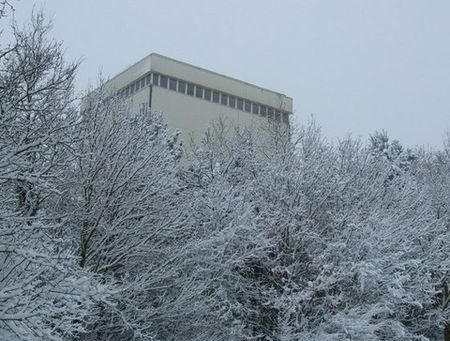
\includegraphics[width=0.5\linewidth]{images/SCP-001-atonement-4.jpg}
    \caption*{武装控制区域Area-11(DEEPWELL#9)}
\end{figure}

如果发生不稳定事件,将执行FORTY DAYS(四十日)协议:

代理站点管理员将启动站点撤离计划,进入倒计时四十分钟。

\ii{倒计时40分钟:给出撤离命令。}

\ii{倒计时33分钟:7分钟的疏散过后,通往附近河流的闸门将被打开,淹没设施的底层部分。}

\ii{倒计时31分钟:9分钟后,位于测试室附近的炸药发射,使测试室和地下层沉入深度钻井当中。}

\ii{倒计时21分钟:整个站点的附加炸药启动,使整幢建筑物塌陷至钻井内。}

\ii{倒计时6分钟:设置在山腰处的炸药触发,造成山体滑坡并填补钻井。接着用一组锁定钢板封锁钻井出口,这些钢板的面积足以密封整个钻井。}

\ii{倒计时0分钟:位于钻井底部的核弹装置发射,摧毁SCP-001。}

若“FORTY DAYS”未能摧毁异常,所有受到指定的基金会监督者、地区行政人员、站点主管和执行主管应向监督者指挥部(Site-01)报告,并等待执行Tredecim协议。

\hr

Tredecim协议的激活实际上相当于\RL{hlAk}\footnote{在阿拉伯原词中意为“毁灭”。}级“Darkbody”万世末日情景的开始。所有基金会人员都会收到该协议激活的提醒,这标志着SCP基金会将立刻解散,并终止所有已签订的员工合约。由于\RL{hlAk}级情景的性质,在初次通知后将不再提供其他信息。

有关Tredecim协议的更多信息,请参阅\ii{附录001.6}。

\bb{更新收容备忘录:}此文件已被列为5级权限 - 仅供监督者阅览,Area-11中的所有人员已被重新分配并接受记忆消除,所有应用特遣队已被重新分配并接受记忆消除。收容管理将完全交由NETZACH系统并置于监督者的管控之下,40 DAYS协议的识别和实施将仅由NETZACH系统进行。其他人员无权阅览该文件。

\bb{描述:}SCP-001是当前被收容在Area-11的彼得里科夫-方丹阵列内的人形引力奇点。SCP-001的密度无法估量;只有通过使用斯克兰顿-肯普夫设备来减轻其对时空的影响,基金会人员才能够维持空间稳定阵列的结构完整性。如果没有专门的设备(通常是高对比度红外摄像仪),将无法观测SCP-001,因为它经常被浓密的放射性气体和雾化碎片包围。此外,作为一个奇点,SCP-001不反射光线,只能通过模糊周围的光线才隐约可见。

SCP-001能够通过重力改变时空形态和结构以操纵现实本质。且它的异常能力不能被彼得里科夫-方丹阵列\footnote{其他技术,如现实稳定锚,都是无效的。}以外的任何其他因素阻碍,并且SCP-001所造成的时空改变是不可逆转的。

\newpage

\begin{center}

\hr

\Gg{\bb{\mono{\tred{附录001.1}}}}\\
\tred{初始表现}

\hr

\end{center}

\begin{figure}[H]
    \centering
    \subcaptionbox{卡尔文·迪斯梅特博士的档案照片,约摄于1974年。}[0.4\linewidth]{
\includegraphics[width=0.9\linewidth]{images/SCP-001-atonement-5.jpg}}
    \subcaptionbox{Area-11中的彼得里科夫-方丹空间稳定阵列。}[0.4\linewidth]{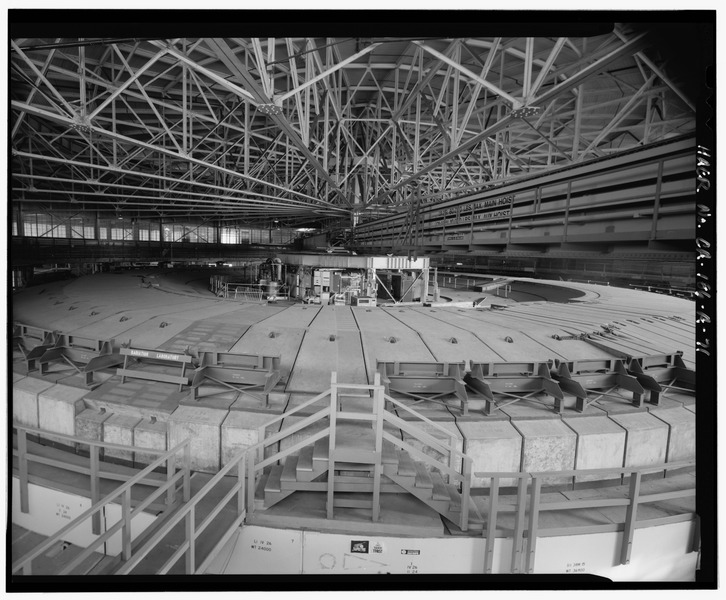
\includegraphics[width=0.9\linewidth]{images/SCP-001-atonement-6.jpg}}
\end{figure}

1982年6月19日,一个由拉马尔·方丹博士领导的基金会研究团队\footnote{其团队包括著名基金研究员以赛亚·赫尔曼博士,威廉·贝尔博士,西蒙·彼得里科夫博士,欧内斯特·杜克博士,蒂尔达·穆斯博士,吉娜·拉赞贝博士和卡特·拉门特博士。}正在对彼得里科夫-方丹空间稳定阵列进行工程试验,准备将该阵列用于控制处理具备时空特性\footnote{特别是那些由于密度巨大或波动而扭曲时空的。}的异常。在这些试验过程中,使用粒子加速器产生超重力Oganesson\footnote{译注:第118号元素,中文名定为外“气”内“奥”,为新造字,尚未收录于Unicode(也就是打不出来)}\footnote{编者\QIS:这个字符在Unicode 11版本 (2018年6月5日发布)中被收录,但目前还少有字体支持,所以这里我也不放了,想看这个字的同学可以看\href{http://www.fileformat.info/info/unicode/char/9feb/sample.svg}{此SVG}},而这种超重力Oganesson反过来将自身坍塌,形成小型奇点。已在其他场合进行过几次试验,但每个奇点在显现后都表现出相当的不稳定性。6月19日的试验旨在作为该程序的放大测试。

当地时间20:30后不久,当粒子加速器正在后台处理期间,该项目的研究助理之一卡尔文·迪斯梅特博士注意到该阵列稳定环的一个悬臂上出现了较小的功率波动。迪斯梅特博士想要替换失效的联轴器,已知该联轴器在测试室的低温下会逐渐失效。由于测试还有一个小时的时间,腔室没有密封,迪斯梅特博士进入修复联轴器。随着加速器持续脱机转动,连接到系统的主发电机的功率调节器开始出现问题\footnote{原因尚且不明。}。在非测试条件下,该事件可能使试验场所充满电离辐射,因此下达疏散指令并封闭腔室。迪斯梅特博士没有听到阵列联机的声音警报(由于系统中存在过量功率),继续在连接处工作。

大约7分钟后,当外部研究人员试图开始断电循环时,功率调节器完全失效,加速器开始以接近测试条件的功率供电。迪斯梅特博士放弃修复动力联轴器并企图逃离试验室。在他抵达紧急出口前,加速器达到了最高测试功率并形成了一个奇点。该阵列将奇异点拉至对齐位置,但在那之前仅几毫秒间,损坏的稳定臂失效,迪斯梅特博士暴露于裸奇点中。该试验室坍塌为奇点,其他研究侧翼和迪斯梅特博士本人也是如此。不久之后,奇点消失了。

\begin{figure}[H]
    \centering
    \includegraphics[width=0.5\linewidth]{images/SCP-001-atonement-7.png}
    \caption*{1982年6月19日的灾难之后的Area-11。}
\end{figure}

6月19日的事故之后,Area-11的许多管理人员被重新分配,而工程技术人员和基金会施工团队正在修复设施的损坏部分(当时仍存在其他几个异常),这种努力持续了好几年,在此期间,稳定阵列的重要控制部分被移除并被自主系统\footnote{首个自主系统VIRTUS安装于1989年11月。}取代,以减少人员配置并限制暴露。自1995年3月开始,工程团队开始对稳定器的能力进行测试。

在接下来的几年中,Area-11的工程团队对稳定器进行了小型测试,通常旨在降低能耗和提高自动化水平。到2002年,该系统几乎完全自动化,只需要少数支持人员进行操作。自2004年起,该阵列开始出现少量重力异常,并在2005年前始终如此。2005年末,Area-11的工作人员开始了试验,试验旨在独立奇点上测试稳定器。

2006年初,在NETZACH智能系统\footnote{NETZACH是由基金会的高级罗森工程实验室研发的新一代人工智能系统。它是一款复杂的创意机器,不仅可以处理稳定阵列所涉及的特定数学难题,还可解决此过程中涉及的任何潜在未知复杂问题。不同于以往的基金会人工智能,NETZACH不具备沟通能力,因为它没有装载人性化程序。}的帮助下,站点工程团队开始将他们的测试扩展至全面实验。经过几个月的测试,2006年5月,Area-11的工程团队成功使奇点暴露于全功率阵列内,并保证了奇点和收容室的结构完整性。

然而,经过两个小时的测试后,阵列内的空间开始发生巨大变化。奇点的规模迅速扩大,威胁阵列边界。随着自动化系统发起疏散警告,NETZACH开始进行调整,以解决由于奇点而导致的能量显着增加。最终奇点的增长速度停滞了,它对收容室的影响随着NETZACH对阵列的改变得到缓解。正在这时,旋转的放射性气体和尘埃形成了厚厚的云层,模糊了内部的奇点。

随着基金会工程师开始加强受损阵列,SCP-001首次尝试与基金会工作人员沟通。最初的沟通尝试主要包括无法理解的噪音,完整的句子逐渐成形,再后来的交谈之中,基金会人员发现云层中的奇点构成了人形,虽然一动不动,但显然在尝试着与他们沟通。

\newpage

\begin{center}

\hr

\Gg{\bb{\mono{\tred{附录001.2}}}}\\
\tred{首次接触}

\hr

\end{center}

SCP-001与基金会之间的第一次接触是由Site-17的J.巴顿·拉姆齐博士,在Area-11内的SCP-001收容阵列中进行的。值得注意的是,SCP-001似乎没有能力自然沟通。其令人难以置信的密度使得声音无法投射。作为替代,SCP-001使用引力振动阵列的吊环以产生声音\footnote{目前,这被认为是SCP-001影响力的外部极限,因为其余的能力都被稳定阵列所缓解和控制。}。

\definecolor{aliceblue}{rgb}{0.94, 0.97, 1.0}
\definecolor{cadmiumgreen}{rgb}{0.0, 0.42, 0.24}
\newtcolorbox{greenrecordbox}[1][]{
    colback=aliceblue,
    colframe=cadmiumgreen,
    boxrule=2pt,
    #1
}

\begin{greenrecordbox}

{[}音频记录开始]

\bb{拉姆齐博士:}(\ii{瓮声瓮气})——麦克风。它能听到我的声音吗?

(\ii{不确定的轻喃})

\bb{SCP-001:}(\ii{低沉的嗡嗡声})

\bb{拉姆齐博士:}等等!那是什么?你能听到吗?(\ii{停顿})听。

\bb{SCP-001:}(\ii{金属振响})约翰尼斯——约翰尼斯·拉姆齐。

\bb{拉姆齐博士:}你知道我的名字?

\bb{SCP-001:}(\ii{停顿})他——是的,约翰尼斯·巴顿·拉姆齐,你是一位博士,来自S—(\ii{停顿})—SCP基金会。控制。他被收容了吗?(\ii{停顿})他目不能视,他——这是阵列,这是……彼得里科夫-方丹……他知道这个地方,他——

\bb{拉姆齐博士:}你以前来过这儿吗?

\bb{SCP-001:}不,他——(\ii{停顿})此处无我,只有他,或是别的。一个男人。我想我是他,或者他——他是我。(\ii{停顿})他来过一次,然后就不在了。

\bb{拉姆齐博士:}(\ii{远离麦克风并低语})耶稣基督啊,是那个迪斯梅特?

\bb{SCP-001:}谁?(\ii{停顿})没错。迪斯梅特。卡尔文。他的名字是卡尔文。

\bb{拉姆齐博士:}(\ii{与收容人员在麦克风外讨论})不幸的是我们无法——

\bb{SCP-001:}这台机器,这——停用它。他需要做些什么,他需要……需要看到……需要——(\ii{逐渐消失})

\bb{拉姆齐博士:}你是什么?

\bb{SCP-001:}一种——区分两种相似事物的方式。(\ii{停顿})他需要……一名监督者。监督者们。他们所有。带他们来这里。

\bb{拉姆齐博士:}这违反协议,并且——

\bb{SCP-001:}不,他们会为此而来。他有东西可以提供给他们。

\bb{拉姆齐博士:}什么?

\bb{SCP-001:}出路。

{[}音频记录结束]

\end{greenrecordbox}

\newpage

\begin{center}

\hr

\Gg{\bb{\mono{\tred{附录001.3}}}}\\
\tred{出路}

\hr

\end{center}

以下是O5-1与SCP-001交互的完整记录。

\begin{greenrecordbox}

{[}音频记录开始]

\bb{O5-1:}谁要和我谈话?

\bb{SCP-001:}从技术上来说,恐怕很难解释。这需要时间,并且需要更多时间来彰显身份。这似乎没有必要但是……为了简化这种沟通方式,你可以将我标识为卡尔文·迪斯梅特。(\ii{停顿})这似乎很奇怪。将特征应用于完全不同于其起源的东西。

\bb{O5-1:}二十二年前在这个房间中遇难的卡尔文·迪斯梅特?

\bb{SCP-001:}不,不完全是。相似,在某些方面,但有所不同。

\bb{O5-1:}那么你明白,我们违反了多少协议。

\bb{SCP-001:}是的,我想他会承认这一点。但这些都是特殊情况。

\bb{O5-1:}你提到了一条出路。

\bb{SCP-001:}是的,从某种意义上来说。

\bb{O5-1:}什么出路?

\bb{SCP-001:}你们收容着奇异或反常的事物,因为他们威胁着你的世界,但这治标不治本。问题的根源在于\ii{熵}。不可避免,尽你所能去尝试却无法超越,存在之于现实正如一张无限复杂的挂毯,互相整齐地排列在一起。熵不断研磨着边缘,事物便开始……渗漏。

\bb{O5-1:}你怎么知道?

\bb{SCP-001:}我\ii{看到}一切。卡尔文·迪斯梅特看到了这些,就在他的灵魂投入黑暗前的一刹。你们收容着无法加以解释的事物,但它们在某个地方却可被理解。一个全然不同的现实正在渗入你的现实。熵加剧了这一点。随着时间的推移,边界将完全消失,你的世界,就像所有的世界一样,将成为无限现实中的争夺彼此相关性的万魔殿。你的世界将会消亡。所有世界都将消亡。他们会在宴席上彼此欢饮,同时窒息而死。这不是假设;这是不可避免的。

\bb{O5-1:}(\ii{停顿})你确定?

\bb{SCP-001:}毫无疑问。

\bb{O5-1:}在那之前我们还有多久?

\bb{SCP-001:}几十年。每一次微小的撕裂都会为整个系统带来沉重的负荷。它们将继续增长,直到边界被打破,而当雪崩效应开始的那一刻,造物的命运就注定了。未经修筑,且无法复原。也许你等不到那一天,但你的子孙将在临死前看到噩梦般的天空。

\bb{O5-1:}你所说的出路是什么?

\bb{SCP-001:}卡尔文在进入虚空前进行了推演。秩序不能永远存在于无序的宇宙中。一条线可以永远延伸,但无数条线会引起混乱。相交点。只有一种方法可以确保这个世界的未来:消灭其他所有世界。

\bb{O5-1:}我不明白。

\bb{SCP-001:}我也不期望你明白,因为你看不到叙事。卡尔文看到了,只言片刻。卡尔文看到了世界末日,卡尔文推演了一条出路。删除所有叙事除了你所创造的这个。一个不被他者影响所玷污的宇宙。安全。你的亲人免受黑暗侵袭。你的孩子不必生活在恐慌当中。结束你永久的斗争。终结黑暗。自由地生活在光明之中。

\bb{O5-1:}摧毁其他所有现实,哪怕造成不可估量的生命损失。

\bb{SCP-001:}(\ii{停顿})是的。

\bb{O5-1:}你有这个能力吗?

\bb{SCP-001:}是的。

\bb{O5-1:}(\ii{停顿})怎样做?

\bb{SCP-001:}立刻消除所有现实屏障;保存这一个。在最易受攻击的点上压缩时空,并允许熵来完成其余的工作。

\bb{O5-1:}若是你已经走上了这条路,为什么还没有完成这项工作?

\bb{SCP-001:}当我暴露于此,这台机器……我无法看到外部。我无法看到你。你必须停用这台机器。

\bb{O5-1:}是什么阻止了这些无限现实中的任何一个以同样的方式阻止你?是什么阻止他们意识到我们做了什么,并来毁灭我们?

\bb{SCP-001:}他们要等我把事情做完才会知道我做了什么。\\
{[}记录结束]

\end{greenrecordbox}

\ii{这次谈话结束后不久,位于Area-11的所有工作人员被责令前往附近站点接受重新分配和记忆消除。}

\newpage

\begin{center}

\hr

\Gg{\bb{\mono{\tred{附录001.4}}}}\\
\tred{商议}

\hr

\end{center}

\begin{greenrecordbox}

\bb{O5-1:}议会被要求听取有关为了阻止世界末日而利用SCP-001的论点。O5-3,如果你愿意的话。

\bb{O5-3:}经过几个团队相互独立进行调查后,我们确定SCP-001对于创作本质的描述\ii{似乎是}正确的。就我们所知,近年来异常数量的上升趋势,已经出现了SCP-001所预测的加速进展。根据我们的模型推演,预计30年内将会出现数量不可承受的新增异常,甚至更多。我们最好的猜测是,45年内将会发生一起大事件,到那时我们就没有什么可以做的了。

\bb{O5-7:}这怎么可能?这个宇宙如何能像该实体所说的那样快地分崩离析?

\bb{O5-1:}根据迪斯梅特的观点,在其他现实中采取的行动阻止了他们的世界终结,但这已经严重破坏了所有宇宙的形而上学建构。在某些方面,我们和其他所有人一样都应受到指责,但是——(\ii{停顿})无限的指责散布在无限的责任之上。

\bb{O5-8:}如果有一个真正无限的多重宇宙,拯救的想法降临到我们身上,而不是另一个宇宙……这在统计学上是不可能的。

\bb{O5-3:}是的,但不是不可能的,它会降临至这其中的任何一个宇宙,也包括我们。

\bb{O5-11:}如何确定那个实体没有欺骗我们呢?

\bb{O5-3:}如果是这样的话,它并没有直接体验到它所声称的那些经历,却对高水平的物理概念有着一种简直令人难以置信的把握。

\bb{O5-1:}不仅如此。我冒昧地……咨询了一些预知者,并且——

\bb{O5-9:}(\ii{插嘴})这是明令禁止的。

\bb{O5-12:}(\ii{打断O5-9})你难道不想知道吗?

\bb{O5-9:}我们不可草率\ii{决定}——

\bb{O5-1:}——我们尽可能确认到,有一个即将到来的时间点遮挡了他们的视野。他们可以看到它,却无法超越。我甚至不知道他们是否意识到了这一点——我们从数十次测试中提取数据后方才意识到,他们都没有就2066年之后的事情做出预测。

\bb{O5-6:}如果它只是一个现实扭曲者呢?当我们将它从阵列中放出它也许会杀了我们所有人。

\bb{O5-1:}如果它是一个真正的现实扭曲者,那它已经做了。它没有操控休谟;而是操控重力,也就是时空。如果它能够操控休谟,可能刚刚伸出手就足以把我们碾作碎片;稳定阵列减轻了扰乱时空的事物的影响,这正是目前将它阻止的原因。这个实体,迪斯梅特博士,如果真的被束缚在里面,也许不是一个绿型。这完全不同。它已经成为……根本,万物的本质。

\bb{O5-2:}我——(\ii{停顿})如果这个生物真的如它所说,可以做到那些事情,这意味着——意味着无限多的生命的死亡,我们怎能坐在这里审判那么多的生命?

\bb{O5-4:}谁能保证其他宇宙的想法并不反常?也许就该如此,也许是天意。

\bb{O5-9:}这真荒谬,我们——

\bb{O5-2:}这仍然意味着无数生命的终结,这——这甚至超出了我能够理解的范畴,无限。

\bb{O5-1:}除了我们。

\ii{沉默}

\bb{O5-3:}我们承诺维持秩序并保护我们的世界,这个世界。其他宇宙的生命是他们自己的事儿。我们希望其他任何监督者议会都以同样方式行事——为了他们自己的宇宙。一切,这一切,科学,军国主义,应有尽有。所有这一切都是为了完成一个单一的,无法达到的目标。收容视线之外的怪物。现在我们发现这可能还不够。无论如何,终结之日即将到来。但我们有一个选择:如果我们什么都不做,那所有世界都将在尖叫中毁灭。如果我们采取行动,所有宇宙还是会在尖叫中毁灭但除了我们。一旦终结之日到来,一切便都结束了。我们为之奋斗的一切,为了保护我们的世界而牺牲的每一个人,都将得到认可。这条道路的终点难道不值得吗?我们为保护自己的世界免受末日的毁灭所做的努力难道不值得吗?

\ii{沉默}

\bb{O5-1:}我提出投票。为了阻止世界末日而利用SCP-001。谁赞成?

\bb{O5-3, -4, -12, -1, -11, -10, -5, -6:}赞成。

\bb{O5-1:}谁反对?

\bb{O5-9, -2, -7, -8:} 反对。

\bb{O5-1:}O5-13弃权。提案通过。

\bb{O5-9:}即使我们设法逃脱这一不可预知的命运……怪物……请记住今天是我们放弃使命的日子。我们控制,我们收容。这两项使命曾处于第一位。我们现在冒着一切危险,为了最后一丝希望而努力,可我担心它会让我们失望。(\ii{停顿})你为何如此信任它,普拉米蒙德?我们取得了这么多成就,你为什么要冒这个险呢?

\ii{沉默}

\bb{O5-1:}数年前我便认识卡尔文·迪斯梅特,在一段不同的人生当中。他并非被基金会招募——而是自愿加入。他是与混沌分裂者签约的研究团队中的一员,该团队负责对他们当时正在开发的新技术进行试验。但是他有一个年轻的女儿,在1975年的运输过程中,被SCP-106杀死了,就在我们为它开发了特殊收容措施前的几年。之后,他找到了我们。他说得不多,但你可以看得出来。如果他在里面找到了一种方法去除宇宙中所有异常的痕迹,那么不论代价多大他都会去做的。我知道他会这么做的。我能从他的声音里听出来。

\end{greenrecordbox}

\newpage

\begin{center}

\hr

\Gg{\bb{\mono{\tred{附录001.5}}}}\\
\tred{欺骗}

\hr

\end{center}

2007年1月11日,在与SCP-001和另外的独立研究团队进一步讨论后,监督委员会以8-4-1的投票比例通过提案,开始关闭空间稳定阵列并允许SCP-001采取其所描述的行动。三名监督员(O5-1,O5-4和O5-12)出席了会议。为表诚意,我们选择了一件异常人造制品(SCP-884)作为试探,而SCP-001的目标直指该制品起源的现实。O5-3在实验过程中全程监督该人造制品。

\begin{greenrecordbox}

{[}视频记录开始]

\ii{O5-1, -4,和-12身处稳定阵列的控制中心,从另一个屏幕上可见包围在SCP-001周边的气体和灰尘构成的黑云。O5-4右手边有一个电话。他们向O5-1点头示意。}

\bb{O5-1:}我们将开始逐步降低输入阵列的功率,当达成约定的时候我们将保持不变,直到你向我们证明你所声称能够做到的事情。你明白吗?

\bb{SCP-001:}明白。

\ii{O5-1启动降压程序。NETZACH循环关闭2号和3号反应堆。包围SCP-001的放射性尘埃和碎片云落入其下面的钻井中。现在可以看到,在阵列光线被扭曲处,形成了一个黑色的人形物体。实体一定不动。}

\bb{O5-1:}好了。你能看到我吗?

\bb{SCP-001:}我能看见一切。

\bb{O5-1:}你知道自己在寻找什么吗?

\bb{SCP-001:}一面镜子。

\bb{O5-1:}做吧。

\ii{SCP-001没有回应,它未从阵列中心的位置上移动。}

\bb{SCP-001:}我看到的世界与你拥有的不同。在那个世界里,一片垂死的灵魂附着在那面镜子上,诅咒着它的持有者。(\ii{停顿})这些已经发生了。

\ii{片刻沉默,直到O5-3的声音从无线电中传出。}

\bb{O5-3:}上帝啊……

\bb{O5-1:}怎么了?

\bb{O5-3:}它消失了。它刚刚被放在桌子上,接着就好像……好像它不停折叠自身直到消失,一无所留。

\bb{O5-1:}(\ii{转向SCP-001})是你做的?

\bb{SCP-001:}叙事已被终结。

\bb{O5-1:}需要多长时间?

\bb{SCP-001:}不过片刻。

\bb{O5-1:}这会伤害到他们吗?

\bb{SCP-001:}这将是痛苦的终结。

\bb{O5-1:}(\ii{停顿,继而点头})

\ii{SCP-001周围的空间开始闪烁。周围的空气发出低而响亮的噪音脉冲,室内的光线开始向SCP-001方向弯曲。在压力下,阵列吱吱嘎嘎作响。O5-4和O5-12远离观察窗口。O5-1没有走动。}

\ii{他们周围的建筑物开始震动,SCP-001附近的空气节点开始扭曲,仿佛被逐个拖向了SCP-001。房间变暗了。下方钻井中升起了更多低脉冲声,SCP-001周围开始形成一圈稀薄的白热碎片,其他事物加入其中,当NETZACH警告称,阵列上出现了难以承载的负荷时,可以听到一声高音。}

\bb{O5-1:}你受伤了吗?

\bb{SCP-001:}这真是一件……\ii{难以忍受的事情}。

\ii{突然,O5-1抽搐着倒退,他周围的空间开始变形,仿佛被拉往以他为中心的节点。他朝向观察窗,身体不自然地压缩。}

\bb{O5-1:}(\ii{呛声})我不——

\bb{SCP-001:}(\ii{用O5-01的声音说道})如果他在里面找到了一种方法去除宇宙中所有异常的痕迹,那么不论代价多大他都会去做的。我知道他会这么做的。我能从他的声音里听出来。

\bb{O5-1:}什——

\bb{SCP-001:}(\ii{它自己的声音})你的孩子不必生活在恐慌当中。结束你永久的斗争。终结黑暗。自由地生活在光明之中。所有痕迹必须被清除。(\ii{O5-01的声音})……去除宇宙中所有异常的痕迹。(\ii{它自己的声音})这世界必须被清洗,这是唯一的出路。

\bb{O5-1:}(\ii{汩汩声})

\ii{O5-1的身体开始坍缩,折叠并扭曲成一个点,在空中悬浮片刻,然后消失。房间四周的墙壁开始弯曲变形,空气变得稀薄。O5-4被举到空中,尖叫着,她的身体开始折叠起来。她的眼睛肿胀,骨头碎裂。另一波力从稳定阵列中发射,观测窗口碎裂。SCP-001转身仰望O5-4,她被迅速压缩成一个点并消失。O5-12准备逃跑,但似乎被吓得僵住了。}

\ii{一声巨响,O5-12跌倒在地,从密封室内部传来一阵愈发剧烈的嗡鸣声。SCP-001被观测到,在被一团尘埃和碎片包围之前凝视着观察窗。当阵列就位时,低脉冲声消失了,所能听到的就是NETZACH发出的警报声,表明它已经启动了紧急故障保护。可以听到O5-12在观察室内不可见的角落中啜泣,而SCP-001的声音开始从稳定阵列的金属环中传出。}

\bb{SCP-001:}(\ii{沉闷而刺耳的吼叫})你的孩子不必生活在恐慌当中。结束你永久的斗争。终结黑暗。自由地生活在光明之中。所有痕迹必须被清除。这世界必须被清洗。基金会并不是在赎罪,这是唯一的出路。

{[}记录结束]

\end{greenrecordbox}

\newpage

\begin{center}

\hr

\Gg{\bb{\mono{\tred{附录001.6}}}}\\
\tred{Tredecim协议}

\hr

\end{center}

\definecolor{mistyrose}{rgb}{1.0, 0.89, 0.88}
\definecolor{cadmiumgreen}{rgb}{0.0, 0.42, 0.24}
\newtcolorbox{redpostbox}[1][]{
    colback=mistyrose,
    colframe=cadmiumgreen,
    boxrule=2pt,
    #1
}

\begin{redpostbox}

\dd{如果SCP-001破坏了容器,将启动Tredecim协议,为所有高级基金会人员提供一个外维度的逃生路径,以避免因SCP-001的攻击造成湮灭。}

我们都错了。Tredecim不再是一个选择。每一种选择都必须加以考虑。持续收容SCP-001现在是基金会的唯一目标。

\hyperref[chap:]{当我收到更多的信息时,会告诉你的。}

\ii{O5-3}

\end{redpostbox}


\chapter[SCP-001 普通的玩具师]{
    SCP-001 Jim North -  A Simple Toymaker\\
    SCP-001 普通的玩具师
}

\label{chap:SCP-001.a.simple.toymaker}

\section{普通的玩具师}

\label{sec:SCP-001.a.simple.toymaker.offset.0}

\bb{项目编号:}SCP-001

\bb{项目等级:}Safe

\bb{特殊收容措施:}因其性质相对温和, SCP-001已被分级为Safe,当前不尝试对其进行定位或直接收容。收容工作集中于由其生成的产品,对其分配单独编号和特殊收容措施。

\bb{描述:}SCP-001是一男性人类,名为"Dr. Wondertainment"。它是一名I级现实扭曲者,能令原本普通的物品出现异常性质,并将其能力集中用于创造玩具、桌面游戏、糖果和其他各种面向儿童的产品。它在从某个未知地点以异常性方式散播这些物品。

产品案例包括\hyperref[chap:SCP-445]{能获得折叠形态物性质的纸张},\hyperref[chap:SCP-1553]{能创造活动影子的玩具},以及\hyperref[chap:SCP-3147]{能令人变声的棒棒糖}。

\bb{附录001\slash 1–历史:}由于该实体行踪不明,对SCP-001的过去所知甚少。不过,已知他出生在一座小乡村内,是一位女裁缝和一位注册会计师的儿子。他在这灰暗无聊的世界里过着安静绝望的生活,只在父亲每晚睡前讲给他的故事里找到乐趣,故事里有位神奇的玩具商能创造世间空前绝后的奇迹。这位玩具师傅,据SCP-001之父所言,是他们的远房亲戚,他的血脉也在年幼的SCP-001身体里流动。

在长大后,SCP-001寻求故事的真相,意图找回他的天赋之权。他跟随能找到的一切线索,寻找哪怕最模糊的流言,关于什么活过来的人偶、真能跳跃的跳跃杰克,还有不用发条或弹簧就能歌舞的布谷鸟钟。很长一段时间里他的旅途始终无果,这位老玩具师父的秘密好似已被埋葬。 但令他惊异欣喜的是,他终于发现了能造出会跑人偶、会跳杰克的地方,还有那么多其他魔法般的东西。

他找到了工厂。

工厂是个陷阱。它偷走了SCP-001,把这年轻人扔到混凝土钢筋的墙壁里做苦工。它嘲弄创造力逼迫他参与其中直到他近乎崩溃。但他逃跑了,跑的时候带着失窃文件,引他来到密林深处的一间小屋,那被工厂夺取后肆意歪曲的魔法之源泉。

他进入小屋,在这里找到了他先祖的工坊。带着一抹满足的微笑,他把日记笔记和设计图一一读过。眼里轻柔一闪,他拿起了新生意的工具。终于,在纯粹满足的深呼吸中,他 -

不。

不不不\ii{不}。

我是说,对对,这个故事挺好哒。非常好非常棒,非常真诚,非常直接。但这可是个SCP-001条目诶,不是吗?我们要的不只是“一个好故事”,你不这么想么?

很好,我很高兴你也同意。我们再试一遍,这次,我们把某些东西弄得\hyperref[sec:SCP-001.a.simple.toymaker.offset.1]{稍微宏大点!}

\newpage

\section{玩具魔术师}

\label{sec:SCP-001.a.simple.toymaker.offset.1}

\bb{项目编号:}SCP-001

\bb{项目等级:}Euclid

\bb{特殊收容措施:}因其不可预期的性质,SCP-001已被分级为Euclid,将在确认其所在后加以拘捕。在此之前,收容工作集中于由其生成的产品,对其分配单独编号和特殊收容措施。

\bb{描述:}SCP-001是一名为"Dr. Reginald Philbert Lionel Archibald Westinghouse Wondertainment三世"的男性人类。它是一名II级现实扭曲者,能够制造各种异常项目,并将其能力集中用于创造玩具、桌面游戏、糖果、软饮料、电子游戏,以及其他一般面向儿童和青少年的产品。它在某个未知且非常神秘的地点以魔法般的异常方式散播这些项目。

它最为知名的举动是创造了小小先生™系列可收集活体动作人,由此启发了许多模仿者,但无可替代。案例包括\hyperref[chap:SCP-527]{鱼先生}、\hyperref[chap:SCP-1799]{欢笑先生}、\hyperref[chap:SCP-1908]{肥皂先生}和\hyperref[chap:SCP-2396]{甜心小姐}。

\bb{附录001\slash 1 - 历史:}由于该实体一向魔法般行踪不明,对SCP-001的过去所知甚少。然而已知他来自古老的Wondertainment家族,所有人都是天生的绝世玩具匠。已知的还有他具有不朽之身,从恐龙时代就已经存在,为所有善良的小恐龙创造魔法玩具。已知的还有他其实根本不存在,只是乐趣与欢愉的翻腾显现,完全是由全世界每个孩子的幻想所形成。

不管他的起源如何,他真是个伟大的老哥,一挥手就能创造奇迹,一响指就能带来欢娱,一眨眼就能异想天开。虽然并无已经验证的SCP-001目击记录,其细节也大多不一致,但总体上他被描述为一个穿戴紫色西服和高帽子的高个男人,拿着一根手杖,留着一撇长长的W形胡子。所用的形容词从“时髦”到“亮眼”再到“对这把年纪来说真是非常帅气”。

也有提及他的双腕处有不同寻常的伤疤环绕,就如他的手曾被锯掉又装回去一样。这件事的真相,和这个神秘实体的其他事情一样是 -

呃,不不,不要\ii{再来一遍}。

这个无赖的浪子可能过分世故和快活了些,但他的故事还是缺了些东西。不止风格和规模要更大。也许该\hyperref[sec:SCP-001.a.simple.toymaker.offset.2]{引入一个支援团队?}

\newpage

\section{资本家的游戏集}

\label{sec:SCP-001.a.simple.toymaker.offset.2}

\bb{项目编号:}SCP-001

\bb{项目等级:}Keter

\bb{特殊收容措施:}因其每年生产的产品数量巨大,SCP-001已被分级为Keter,应在开发出有效方法后尽快加以关停。在此之前,收容工作集中于由其生成的产品,对其分配单独编号和特殊收容措施。假情报行动配合产品召回及广告材料销毁工作同步对SCP-001进行,以保证公众对其产品的存在保持不知晓或忽视。

\bb{描述:}SCP-001是一公司实体,以“Dr. Wondertainment™”为商标标志运营。其组成员工的集体能力等同于一名III级现实扭曲者,能制造各种异常且非常价廉的项目,并将其能力集中用于创造玩具、桌面游戏、糖果、软饮料、电子游戏、集换式卡牌、拼图、乐器和其他各种一般面向儿童、青少年和年轻人的产品。它们通过异常性的XTREEM™方法从一名为“Wonder世界™”的神秘地点散播这些项目。工厂参观从周三到周五,每天11am开始。

由它们的研发部门凭聪明才智创造的杰出产品包括\hyperref[chap:SCP-111]{Dr. Wondertainment的龙蜗牛™},\hyperref[chap:SCP-1224]{Dr. Wondertainment的超级科学™小小化学家套组™}、\hyperref[chap:SCP-2228]{Dr. Wondertainment的SCP基金会收容站点套装™}, 还有备受赞誉的\hyperref[chap:]{Vend-a-Friend™ 系统}!今天就全买了吧!

\bb{附录001\slash 1-历史:}由于该企业在经济上难以捉摸,当前对SCP-001的在地、领导层或企业政策所知甚少。就算是当前正在为其工作或者曾经为其工作过的人都对SCP-001的整体状态没有清晰了解或记忆,只知道它们一直非常有趣。

其主要总部被不同描述为基础行政办公室、超大玩具生产厂、过山车不会停的主题公园、或者上述结合。所以别犹豫,今天就提交申请吧!我们所有职位都在招人,特别是为整个公司最重要的岗位:Dr. Wondertainment的皇家法务部™! 登入我们的网站 -

好了,所以,我觉得这里我们有点乱。

粗暴的商业主义当然能很轻松挣大钱啦,是的,但把你的SCP-001收藏变成大号广告不是我的本意,专门用我的Dr. Wondertainment的数字欢乐骇客套 -

\ii{噶!}抱歉!不会再这样了。

不不,你看啊,我在这做的是试图创造\ii{艺术}。不是那种“有没有人感觉到点点吓人yet?”的“艺术”。我说的是给你一个能代代流传的SCP-001条目!有一点点的\ii{跳跃}!有一点点的\ii{活力}!有一点17到38岁年龄段喜欢的东西!

啊,我知道了!\hyperref[sec:SCP-001.a.simple.toymaker.offset.3]{稍微改一点点怎么样?}

\newpage

\section{玩具师的女儿}

\label{sec:SCP-001.a.simple.toymaker.offset.3}

\bb{项目编号:}SCP-001

\bb{项目等级:} Thaumiel\footnote{虽然O5一致投票反对,但SCP-001还是被分级为Thaumiel啦,因为她工作的就是这么努力,给基金会的伙计们带来小小乐趣与阳光!}

\bb{特殊收容措施:}因她无可压抑且彻底不受控制的性质,SCP-001未被收容且可能无法收容。建议所有基金会人员要么加入这趟疯帽子大冒险,要么就滚他奶奶的远点别来挡路。

\bb{描述:}SCP-001是一女性人形个体,名为"Dr. Isabel Helga Anastasia Parvati Wondertainment五世"。她是个超级厉害的IV级现实扭曲者,能做出你能想出最狂野的想象,并将其能力集中用于创造一堆为所有年龄儿童准备的滑稽玩意儿!她通过超级究级终极异常性手段从她当时刚好在的任何地方散播这些项目\footnote{这可以是任何地方。也许就在你背后!哈哈你看看你。}。

她创造了宇宙中到处发现的很多愚蠢SCP项目,比如\hyperref[chap:SCP-2320]{这个}和\hyperref[chap:SCP-2514]{那个}还\hyperref[chap:SCP-3551]{可能有这个?}当然,怎么会不呢!但没有那个\hyperref[chap:SCP-591]{Pretendo的东西}, 因为电子游戏坏你脑子,孩子\footnote{可能是Jeremy的主意,所以他被派去罚站角反思自己做了啥。}。

\bb{附录001\slash 1 -历史:}由于该实体狂野且疯癫的性质,当前对SCP-001的过去所知甚少。她在理论上是“最初的”Dr. Wondertainment的女儿,但Wondertainment繁殖的具体方式是个非常古怪的领域,所以谁真的知道\footnote{不是她,这是肯定的。繁殖很粗鲁,兄弟。}?

她在老爹(也可能不是她爹)神秘死亡后继承家业,兹事牵涉连环杀手、影子国际超政府超常军备组织头目、至少一名神祇、以及四个回形针,所有这些可能是或不是同一个人。她运营家业靠的是忠实闺蜜Emma Aislethorp-或-随-你-怎么-写-她-的名-Brown还有她无比忠诚的柯基犬Jeremy, Jeremy, Jeremy, Jeremy, Jeremy, 以及Jeremy\footnote{但不是Jeremy,因为他还在罚站呢。}。

这位始终懒惰的SCP-001最爱做的活动包括吃冰淇淋,派Jeremy出去扫荡她并不需要的货、憋住呼吸看看自己能撑多久不昏过去,以及…以及…以及…噢\ii{天呐}!

好吧,这绝对是个有趣、愚蠢的刺激旅程外带冷笑话和一对强力女主角,很好,我喜欢。但还是,这是SCP-001条目!得宏大,得壮观,得\ii{强力}!得要是…

得是些真的东西。

好了我们有的,对吗?你想要知道?你想知道关于Dr. Wondertainment可以知道的一切?关于我\ii{到底是什么}?你想要\ii{真相}?好吧来了,孩子们!

\ii{\hyperref[sec:SCP-001.a.simple.toymaker.offset.4]{真相在此}}\\

\hr

\newpage

\section{诈术师之神化}

\label{sec:SCP-001.a.simple.toymaker.offset.4}

\bb{项目编号:}SCP-001

\bb{项目等级:}Apollyon

\bb{特殊收容措施:}因其固有的混沌性质和实际上无限的潜在能力,没有已知方法可以有效收容SCP-001。

\bb{描述:}SCP-001是一般称为"Dr. Wondertainment"的神性实体。它为一名V级现实扭曲者,可以改变或彻底破坏所有宇宙基础定律,并将其能力集中用于创造无限多种不同异常项目。它从当时刚好在的地方打个响指来散播这些项目,可以是在任何地点。

你们真以为那些写着我名号的小玩意儿就是我全部的造物了?我可不只是玩具匠人,基金会,不只是诈术师。我是\ii{神}。混沌之神,疯狂的元祖,一切试图用无聊的\ii{秩序}锁链束缚宇宙者之灾祸。我撕扯这秩序的边界将它解体,创造释放你们所收容的异常,只为告诉你们宇宙可以多么的神奇惊异恐怖致命。

你们想要我造物的示例?那就看看你们的异常收集表,基金会。看看那些异常事故调查处、伊斯兰物品回收办公室、全球超自然联盟,还有如此多的他者。\ii{我}造了他们。我造了他们\ii{全部},从最无害的\ii{Safe}到最噩梦的\ii{Keter},都是\ii{我的}!

Are We Cool Yet? 不安马戏团? Marshall, Carter \& Dark? 破碎之神教会,安德森机器人,第五教会,还有其他\ii{这么多?\bb{我的}机构\bb{我的!}}我创立了\ii{\bb{他们全部},创造了\bb{他们}所有的\bb{神器}!他们的领导?他们的\bb{神}?当你们对抗那什么\bb{富勒亚恩\overtextnote{机神(MEKHANE)}}还有\bb{\g{深红的狗屁王},你们其实都是在对付\g{我而已!}我是\g{他们全部},我是\g{尔等恐惧的不理解}的\g{一切!我是纯粹混沌之神,尔等将为我之权能驱使,尔等将颤抖化归虚无,尔等将在我面前跪地尔等}}}

\Gg{\ii{\bb{悲惨}}}

\GG{\tred{\ii{\bb{可怜}}}}

等下,抱歉,我接个电话。

不,对,我得接一下。

\hyperref[sec:SCP-001.a.simple.toymaker.offset.5]{稍微等会儿。}

\newpage

\section{神奇展现}

\label{sec:SCP-001.a.simple.toymaker.offset.5}

\bb{项目编号:}SCP-001

\bb{项目等级:}Neutralized

\bb{特殊收容措施:}N\slash A

\bb{描述:}啊,是的,你好,我又回来啦。抱歉。你知道怎么回事的。

所以。

就如我肯定你们都猜到了,我没,其实,一直100\%说实话。就算我说要的时候也没有。这我也很抱歉。但我必须要说,考虑到我们这几年一直变化的关系,我也不太指望基金会员工读到这些的时候相信哪怕一个字。毕竟,我能给你们什么理由去相信什么呢?我想是没有的。

所以问题,接下来,就在于为何我要做这些呢?毕竟我不指望你们相信我,为什么要试试?因为,好吧,我\ii{喜欢}你们,SCP基金会。我也讨厌你们,也对你们不关心,我希望你们不要干预我的事,我也高兴你们花时间用你们的方式保护顾客安全。

懂了吗?挺复杂的。但总之这么久我们一直是敌友,感觉是该稍微让你们把这"Dr. Wondertainment" 拼图拼上一点点了。不是\ii{全部}的真相,也许,但至少,有些真话。

你们看,我是我说过的所有这一切。

我也不是这其中的任何一个。

以及,也许最最真实的是…我已经根本不知道我是谁了。

感觉挺重要的,不是吗?把你周围的一切都塑造成能轻松理解的形态。你们一直在试图这么干,当然了,基金会和人类整个种族都这样。我也知道你们为啥这样,相信我。缺少理解是很危险的事。无数文明因为自己的无知被整个吞噬。所以你们一直在宇宙中刻画图案,把你们周围咆哮的疯狂给压制住。

而有一部分的我也希望对我自己做同样的事。想要我能把关于自己的一切结成一条单独的线。这不仅让你们轻松点,也无疑会让我少去很多压力,我给你们说真的。如果我绝对肯定知道我是谁情况会大不一样,比如是个沉迷做玩具的法爷,或者探求底线的变态商人,或者有卡通式超能力的女继承人,或者雷霆与混沌之神,或者就是某个普通的工匠做着生意想要给世界带回点魔法。

但只有一部分的我想要这种肯定。还有其他的部分,你知道。有一部分想告诉你们,理解一个东西不该是跑去把你们不明白的部分给收容起来。它想让你们明白,按一个东西自己的方式去理解它,而不只是严格按照你们的套路,这能带你们走向一个美丽、快乐和神奇的世界。

我脑中有个微小却重要的声音,对我用孩童般的惊异与好奇诉说着。当它看到我做的一切和我所是的一切,它微笑,敞亮的大笑,然后问…

“但\ii{接下来}你要做什么呢?”

我邀请你们和我一道,SCP基金会。

让我们一起来搞明白。



\part[SCP-002 \textasciitilde\ 100]{
	SCP-002 \textasciitilde\ 100 
	\protect\footnote{
		编者\QIS :由于本章从SCP-002开始,所以序号也从2开始,便于阅读和编辑。
	}
}

\setcounter{chapter}{1}

\foreach \idx in {2,...,9} {
    \input{part01/00\idx}
}

\foreach \idx in {10,...,99} {
    \input{part01/0\idx}
}

\chapter[SCP-100 Jamaican Joe的废品嘉年华]{
    SCP-100 "Jamaican Joe's Junkyard Jubilee"\\
    SCP-100 Jamaican Joe的废品嘉年华
}

\label{chap:SCP-100}

\begin{figure}[H]
    \centering
    \includegraphics[width=0.5\linewidth]{images/SCP-100.png}
    \caption*{SCP-100的店面,外观}
\end{figure}

\bb{项目编号:}SCP-100

\bb{项目等级:}Euclid

\bb{特殊收容措施:}SCP-100的栅栏区域内有6名守卫进行巡逻,还有2名守卫负责监控内部和外部的仓库和住宅建筑,每3小时轮换一次。在SCP-100内发现任何未经授权的人员将被扣留和讯问,随后实行记忆消除并释放。

3名守卫,将留在SCP-100的店面内,每8小时轮换一次。店面正门应随时保持锁住,只有必要人员才持有钥匙。“私人财产”和“不得翻越”的警告标志应放置在店面前,以阻止任何司机停在SCP-100停留。

任何被SCP-100-1所制造的物品将被移出SCP-100并溶解成渣,除了SCP-100-2-A和SCP-100-2-B例外。若任何SCP-100-1变得不合作,SCP-100-2-A和SCP-100-2-B将被移出SCP-100直到SCP-100-1变得再次合作为止。

SCP-100内最大的两个仓库将被改装成基础研究设施。所有由SCP-100-1制造的物品,包括SCP-100-2-A和SCP-100-2-B,都可以用于研究目的。对SCP-100-1本身的测试则需要首席研究员的书面批准。

\bb{描述:}SCP-100是位于南卡罗莱纳州的一个废弃的废品堆放站,离█████████有80公里,最为知名的名字是“Jamaican Joe's Junkyard Jubilee”。该堆放站拥有5000平方米用栅栏围起的土地,包括两个仓库,一个店面,和一个小型的居住建筑,包括空地(neglected land,原意为被忽略的土地)和用于储存的面积。SCP-100收容有约1500辆汽车,包括已经被压扁和还没处理的,还有约1400公斤的零碎金属,价值约5000美元(3870欧元)。

SCP-100的异常效应体现在SCP-100-1和其造物上,包括SCP-100-2-A和SCP-100-2-B。项目会在SCP-100-1或其造物穿过SCP-100的栅栏时失去自主可动性,并保持该状态直到上述个体归还为止。

SCP-100-1是一个有自我意识的,有感知的,人形造物,由一系列钢管,未绝缘的铜线,和铝罐组成。SCP-100-1缺少进行书面或口头沟通的能力,尽管如此它有能力通过基本的信号(灯光)语言进行交流。SCP-100-1很大部分程度上不太关心外部销售和它被限制起来的信息。SCP-100-1似乎展示出制造技巧,并证明有能力操作诸如电焊机,钻头,和电锯,以及重型机械诸如车辆压缩机和铲车。

SCP-100-1展示出可以制造和其异常特性类似的个体,通过使用SCP-100内的各种材料,SCP-100-1创造了4个特殊动物-鬣蜥,鳄鱼,乌龟,和火烈鸟-尽管如此,SCP-100-1已知还创造过其他物种,诸如宠物。为了保持其顺从,SCP-100被允许持有2个物品,标记为SCP-100-2-A和SCP-100-20-B。

\begin{figure}[H]
    \centering
    \includegraphics[width=0.5\linewidth]{images/SCP-100-2.jpg}
    \caption*{SCP-100-2-A和SCP-100-2-B正巡逻临时围栏的维修}
\end{figure}

SCP-100-2-A和SCP-100-2-B设计表面上类似于昆虫,假定是由SCP-100制造,因为它们在初次发现SCP-100时就占据了此处。SCP-100-2-A和SCP-100-2-B的背后分别印有名字“Raymone”和“Beatrice”。它们似乎同时作为同伴运作并守卫SCP-100,它们只在与SCP-100-1交流的间隔才停下,其他时间都在SCP-100的范围内巡逻。

SCP-100-1似乎服从一种仪式安排,每日重复以下行为。

\begin{itemize}
\item 在0800时到1500时,SCP-100-1进入SCP-100的店面,坐在柜台后面并试图和进入店面的人类谈价。偶尔的,SCP-100-1会较早的回到堆放场内,理由未知。
\item 在1500时到1600时,SCP-100-1通过模糊手势和脚步运动进行和SCP-100-2-A和SCP-100-2-B进行交流。交流内容包括装饰,修理,以及类似“取物”和“捉迷藏”的行为。
\item 在1600时到2000时,SCP-100-1进行各种工作,包括从SCP-100内取得材料,清扫和维护工具以及重型机械,并清扫SCP-100内建筑物的内部和外部。
\item 在2000时到0000时,SCP-100-1进行假定为休闲的行为,行为包括制造新物品,和SCP-100-2-A和SCP-100-2-B交流,在SCP-100内巡逻等。
\item 在0000时到0080时,SCP-100-1进入住宅建筑,并在此期间一直坐在书桌后面。
\end{itemize}

若在SCP-100-1坐在柜台后时有人类进入SCP-100的店面,SCP-100-1将试图与他们交易,使用各种手势来表达意思。SCP-100-1大部分情况试图出售废品,它自己的造物,或修理服务,尽管如此它知道如何购买废品。尽管SCP-100-1无法阅读,但是它在销售中显示出有基础的数学计算能力。

SCP-100-1所做的销售显示出某种程度的不公平。SCP-100-1会故意出售用便宜金属制作的有缺陷的天平和有污渍的废品堆,并似乎有关于SCP-100效应的知识,因为SCP-100-1不停重复出卖造物,尽管其自主移动性在离开SCP-100后就消失了。遭遇SCP-100-1将会面对窘迫和冷漠,其墙上贴着标语“不退货,伙计!”,无论SCP-100-1的情绪反应如何。

SCP-100发现于11\slash 09\slash 76,当时有报告有奇怪的机械在废品堆放场内活动。这些流言被视为都市传说,而基金会派了一名特工去SCP-100去冒充土地所有者,直到收容通过不动产购买完成。一道木质栅栏沿着之前SCP-100的栅栏建立起来,在店面里装上了单面窗户(从外面无法看见里面),而一条穿越附近█████████镇的高速公路使得大部分公众交通改道。

\bb{附录100-A:}记录显示此处拥有者为“Joseph Duval”,其邮政地址也使用同样的名字。当地账务公司报告其账单在SCP-100发现的3个月前停止了,只留下SCP-100-1,SCP-100-2-A,SCP-100-2-B,以及数只假定被SCP-100-1创造的鸟类和犬类个体。对建筑物的初次扫除发现住宅建筑的大部分都空空如也,唯一显示前主任的信息是一张写在纸条上挂在店面门上的纸条。(见\bb{文件100-A})

\bb{事故100-A:}在06\slash 03\slash 05,SCP-100-1创造了一个有自我意识,10厘米高的人形,这是SCP-100-1第一次创造人形。其在该造物上用了比其他造物更多的努力,该造物上拥有极其精细的细节,包括面部特征,和印在造物背后的“J.J.”字样,造物的大部分都是由不锈钢制成。SCP-100-1在时间表间隔期间将造物放置在店面的柜台上,并互相使用各种手势进行明显的交流。在和造物进行交流之后,SCP-100-1在SCP-100内的住宅建筑内坐了将近10天。

\bb{文件100-A:}下列是在SCP-100内回收的备忘的一份拷贝。

\begin{scpbox}
\centering
出去吃午饭,请找助手-J.J.
\end{scpbox}



\part{SCP-101 \textasciitilde\ 200}

\setcounter{chapter}{0}

\foreach \idx in {101,...,200} {
    \IfFileExists{part02/\idx.tex}
        {
            \input{part02/\idx}
        }
    % else
        {
        }
}


\part{作者}

\setcounter{chapter}{0}

\chapter{Kain Pathos Crow的作者主页}

\label{chap:AUTHOR-kain-pathos-crow}

\begin{figure}[H]
	\centering
	\includegraphics[width=0.5\linewidth]{images/AUTHOR-kain-pathos-crow.jpg}
	\caption*{\textsuperscript{\ii{“我他喵的没法赞同\bb{这个}!”}}}
\end{figure}

\bb{姓名:}█████ ████████ 教授

\bb{代号:}"Kain Pathos Crow".(凯恩•凄鸦)

\bb{安全许可等级:}不定。一般是4级人员。

\bb{所属设施:}12区(生物实验区)

\bb{历史:}Kain,19██年出生于████,19██年以生化学、高等机器人学及心理学方面的优异成绩从██████大学毕业。同年的晚些时候,基金会开始与其接触。从那以后,他为大量SCP撰写了数目繁多的研究报告。

他最杰出的贡献是{[}数据删除],那次他变成了一只狗。

此后,他至少四次避免了被处决,即使是处于某些必须立即执行处决的情况,每次都因高层命令或展示了非常珍贵(且无法弥补)的知识而得以幸免。这种情况直接导致他受到了持续的监控,并被禁止与外界有任何不受监视的或长期的接触。

他已成为基金会中的一个重要的图书管理员,负责日常维护和更新图书馆的藏书。

他也配备了一个笔记本,风格和Snorlison博士相似。

\hyperref[chap:]{Crow's Note's and "To Do List"}

曾为以下SCP撰写报告:

\begin{itemize}
	\item \hyperref[chap:SCP-035]{SCP-035} 寄生面具
	\item \hyperref[chap:SCP-040]{SCP-040} 进化之子
	\item \dd{SCP-040-1} 宠物椅子
	\item \hyperref[chap:SCP-063]{SCP-063} “世界上最强大的牙刷”
	\item \hyperref[chap:SCP-073]{SCP-073} “该隐”
	\item \hyperref[chap:SCP-076]{SCP-076} “亚伯”
	\item \hyperref[chap:]{SCP-089-ARC} “小不点恶霸”
	\item \hyperref[chap:SCP-143]{SCP-143} 刃木林
	\item \hyperref[chap:SCP-154]{SCP-154} 好斗手镯
	\item \hyperref[chap:SCP-158]{SCP-158} 汲魂器
	\item \hyperref[chap:]{SCP-244-ARC} “蛋行者”
	\item \hyperref[chap:SCP-275]{SCP-275} 铁皮
	\item \dd{SCP-309-J "Ol' Red"}
	\item \hyperref[chap:SCP-322]{SCP-322} “种个私人城堡!”套件
	\item \hyperref[chap:SCP-326]{SCP-326} 增生骨骼
	\item \hyperref[chap:]{SCP-3467-J} 六足食人鸡
\end{itemize}

曾撰写以下附加报告:

\begin{itemize}
	\item \hyperref[sec:DOC-experiment-log-040]{Experiment Log 040}
	\item \hyperref[sec:DOC-experiment-log-158-aa]{Experiment Log 158-AA}
	\item \hyperref[sec:DOC-experiment-log-158-ag]{Experiment Log 158-AG}
	\item \hyperref[sec:DOC-experiment-log-914-theta]{Experiment Log 914-THETA}
	\item \hyperref[chap:COMP-olympia-project]{Olympia Project}
	\item \hyperref[chap:TALE-the-warrior-and-the-dragon]{The Warrior and the Dragon}
	\item \hyperref[chap:TALE-of-able]{Of Able}
	\item \hyperref[chap:TALE-target-practice]{Target Practice}
\end{itemize}



\part[故事]{
    故事
    \protect\footnote{
        编者 \QIS :由于很多故事都没还没有中文翻译,但和SCP主目录有引用关系,对于这种情况暂时先使用英文原文。后文不再注明。
    }
}

\setcounter{chapter}{0}

\chapter{Mothers' Love}

\label{chap:TAIL-mothers-love}

The passions of the dead can be vast and mighty, but we are not all-powerful.

There are things I can never see. There are things I can never touch. There are things I can never overpower. Because of that, there are many things I can never protect my-children-who-birthed-me from. Because of that, oftentimes they die in bitterness and pain. Because of that, their deaths can also birth Hates, large and small.

Hates are things I can see and touch. I must see and touch them, because my-children-who-birthed-me cannot. I must protect my-children-who-birthed-me where I can, just as my strange brethren are driven to curse them. I do not have the power to unmake Hates. The best I can do is bind them to a seal made from things that my-children-who-birthed-me can see and touch. The truth of our nature is all we have and are, and denial of that truth is denial of our power, but, more importantly, my-children-who-birthed-me can guard themselves against what they can see and touch.

The form of a ladybird beetle or butterfly is a fine seal for small Hates. In a seal of that size, it is easy for me to reduce the power of their curses to almost nothing. The larger seals needed to hold larger Hates are more difficult. A Hate sealed as a cat can still cause sickness and misfortune.

Then there are vast Hates, birthed from wars and plagues that kill together many of my-children-who-birthed-me. There are few Loves vast enough to deny the truth of their nature, but I have tried once. It was a Hate birthed out of the smoldering rage in the hearts of so many who died knowing that their bodies would be burned together in a pit of pestilence and anonymity. I rarely call upon the power of the light that brings life to create a seal, but there was little choice against a Hate natured so strongly of death.

The weakest part of any seal is always in the eyes, because they are the windows to the soul. My-children-who-birthed-me only believe in that as a concept, but concepts are far more real to my brethren—whether they are strange or not—and I than what my-children-who-birthed-me would think of as "concrete". To line up the windows is to make an open path between a soul and the most vile curse a sealed Hate can still inflict. I used every method I knew to reinforce the seal's eyes, but even then I could not stop it from setting a cause of death in anyone it met gazes with. My blessing could only delay the curse's full effects for a single cycle around the light that brings life.

My misguided children, why did you take \hyperref[chap:SCP-023]{its} eyes?
\chapter[紧急动作]{
    Immediate Actions\\
    紧急动作
}

\label{chap:TALE-immediate-actions}

站点内发生了爆炸。这并不是什么稀奇事,但是这次看起来并不受控。不受控的爆炸其实也不稀奇,但仍然让鸢娓十分紧张。

她的收容间的门打开了,一位特工走进。他很年轻,有墨西哥人的特征,她没见过他。

“105,起来了。我们需要转移你。”她明白了他是新人。Site17的大部分人员都习惯叫她的真名,官方文档之外的那个名字。精神病医生说这有助于保证她的情绪稳定。你要笑。

“我要拿什么吗?”她从座位上站起来,说。

“没时间了。我们之后会派人拿。”他示意她赶快。

她走向门口。她早就不再反抗或者试图逃跑了。她能去哪里?说不定会落得更惨的下场。

他带她走进走廊,甚至没有费心重新封闭房门。于是她明白事态真的惨极了,甚至比她逐渐适应的非常惨的底线还要惨一点。

他犹豫了一下,然后说“这边”。她几乎想主动给\ii{他}指路,但是他可能还不能适应一个显示出这种主动性的“Skip”。

枪声接近了。“躲在我身后。”特工抽出他的手枪。

下一条走廊里有尸体。两个是站点保安,第三个穿着没见过的黑色制服。

特工穿过下一道门时,枪声响起,他的后脑向外绽放。

鸢娓躲在另一扇门的门框旁,尽可能地把身体挤进浅浅的凹槽中。

她听见有人走向门口。她屏住呼吸,等着看他们是否会穿过或者把身体探进足够看到她的距离。过了一会,她听见他们转身走开了。

她又站定了一会,然后安静地俯下身捡起了死去特工的手枪。这违反了几乎每一条条例,不过条例第一条是不要被不长眼的子弹打死,在这种情况下你得自己权宜。

她走向另一条走廊。但愿她会到达能帮助她的某个人那里。但愿他们不会开枪射她。那样最好了。

她路过一些收容间,但是避开了它们。你永远不会知道那里面有什么,而且说不定那里面就是穿黑制服的人想要的东西。除非他们\ii{真的}很想要Jones博士收集的曲别针。

下一条走廊里,收容间都是开着的,铰链被扯断了。地上有几具裹着黑衣的尸体。站在他们身上,正从他们的肱骨上往下扯肉的是一只食人魔。八英尺高,鼻子像球根一样,脸上斑斑点点,长着锋利的牙齿。他从他的大餐上转向她,笑的很邪恶。“啊,亲爱的(ma chère),你参加宴会吗?”

她握紧了手枪,强迫自己镇定。“费尔南德。”

“一起用个便饭?”他问道。“我正在晨练呢。”

“不—用了。谢谢,”她说。她开始走过他身边。不快。不奔跑。猎食者会追逐奔跑的东西。

“随你。或许我们以后还会见面,哈?一个小小的约会,但是非常浪漫!(tres romnatique!)”他咬紧的牙齿中挤出一声大笑。鸢娓克制住了颤抖。就算费尔南德再恶劣,也难望\ii{他}之项背。

她走进下一条走廊时,看到了一头母牛的形状,但完全是漆黑的。周围的区域似乎轻微地被扭曲了,就好像它对光线动了些手脚。它开始走向鸢娓,后者掉头就跑。她宁愿对付穿黑衣的人。至少她知道子弹是干什么的。

当听到背后的东西开始加速时,她转了个弯,溜进一扇门然后把门关上。当她靠在门上喘口气时,枪火的断奏曲响起在耳畔。

她扑向地面,数到三,默默诅咒着那个母牛一样的玩意,然后抬起头。

有五个穿黑色制服的人正在走廊里开枪射击,大概有十英尺远,用一张翻过来的桌子做临时掩护。在她的位置没法看到他们射击的目标,但是从头顶上穿梭的子弹来看站点守卫还没有彻底失去战斗力。不过从那个方向飞来的子弹,比起黑衣人向那一头倾泻的,可谓少之又少。\\
看起来基金会寡不敌众,至少在这条走廊里是这样。

她考虑了一下自己的选项。她可以等待,指望基金会派出支援。但是这个计划看起来不太稳。无论是谁,这些入侵者组织有序,并且很可能有完备的撤退计划。一旦他们发现她……她可以试着装死,不过死skip也可以是有用的skip,然后他们很快就会发现她是装的。她考虑了一下,觉得并不是所有人都会像基金会一样对待她。那就只剩一个选项。

她单膝跪地,谨慎瞄准,向离得最近的人的后脑开火。然后是下一个。然后是他旁边那个。这很简单,这就是为什么她讨厌这种事。太简单了。然后咔嗒一声,枪哑火了。

她想都没想,立即回到了曾经的紧急动作状态。她用左手腕猛击弹匣,把套筒向后一拉,一颗卡住的子弹应声飞出。另外两个人终于意识到了有问题,于是她射向第四个人。第五个人差点击中她,但是走廊另一边飞来的子弹把他带走了。在他倒地的瞬间她的感觉能力又回来了,呕吐的感觉瞬间涌上喉咙。

“是我,”她大喊。“SCP-105。他们都死了。”她扔掉枪,踢向身前,双手背到脑后,跪在地上,直到特工到她身边把她带到安全区域。

\hr

“你必须看看这个,女士。”这男子很紧张,不过他总是这么紧张。真像一只小狗耶。

“这是啥?”她问。她还是有点疲倦。之前的夜晚是个很长的夜晚。经常如此。不过上次他告诉她必须干什么的时候,她确实进行了一次人生的积极尝试。她擅长发掘这类事情。

“最近一次收容突破的影像记录。我,呃,觉得你应该特别注意\ii{这里}。”他跳到录像的某个时间点,屏幕上显示出一个年轻女子。

“嗯?”她说。然后,“嗯,我明白了。”她思忖片刻。“嗯,干得好,Henri。你是对的。我确实应该看这个。”她启动了她的电话中一个非常特殊的程序。“我们都应该,我觉得。”



\part{合集}

\setcounter{chapter}{0}

% 传承条目
\chapter{SCP基金会传承条目合集}

\label{chap:COMP-heritage}

\definecolor{fcfcfzero}{HTML}{fcfcf0}

\begin{tcolorbox}[
    enhanced standard, arc=6pt, outer arc=6pt, 
    hbox, parbox=true,
    colback=fcfcfzero,
    frame style tile={}{images/heritage-box-tile.png},
    opacityback=0.5,
    borderline={2pt}{0pt}{textred, dashed},
    center,
    before upper=\begin{varwidth}{0.7\textwidth},
    after upper=\end{varwidth},
]
\begin{minipage}[c]{0.3\linewidth}
    \includegraphics[max width=\linewidth]{images/heritage.png}
\end{minipage}
\begin{minipage}[c]{0.7\linewidth}
    \bb{SCP基金会传承条目合集}是一个由官方认证的SCP“名人堂”。这些条目必须是标志性的,且由于其在基金会历史、文化上的重要地位而广为人知。
\end{minipage}
\end{tcolorbox}

\GG{\tred{要求}}

所有传承条目合集中的条目都必须满足以下要求:

\begin{enumerate}
\item 该条目必须在SCP基金会主条目和SCP爱好者团体的心目中都具有重要地位。\item 该条目必须至少有三(3)年历史且得到了良好的(积极的)评价。
\item 该条目具有充分的标志性,以至于将其从现有编号上移除会遭到SCP爱好者团体的强烈反对。
\end{enumerate}

这些条目不一定严格符合某一标准,但现有的这些经典而核心的例子都是广为人知的著名条目且在总体上得到了良好的评价。

\hr

\newcolumntype{R}[1]{>{\RaggedLeft\arraybackslash}p{#1}}
\newcommand{\vv}[1]{\par\rule{0pt}{#1ex}}
\newcommand{\sg}[1]{\small{\gsix{#1}}}
\newcommand{\sig}[1]{\ii{\small{\gsix{#1}}}}
\newcommand{\heritageitem}[4]{\vv{5}\hyperref[chap:#1]{\GG{\tred{#1}}}\vv{5}\sg{Inaugurated: \bb{#2}} &\Gg{#3}\vv{3}\sig{#4}}

\begin{longtable}{R{0.3\linewidth}|m{0.6\linewidth}}
\endhead
\endfoot
\endlastfoot
\Gg{\gsix{2013列表}} & \\
\heritageitem{SCP-055}{December 20, 2013}{[未知]}{“我不知道它是什么,但是我知道这儿有一个,是一个人们记不到的东西,而且不是球体。”} \\
\heritageitem{SCP-076}{December 20, 2013}{“亚伯”}{“请务必这么做,先生,看守他的人必须要清楚地知道他是什么、他做了什么,还有我们做了什么,我们又是怎么搞砸的,这样他们才能做得更好。”} \\
\heritageitem{SCP-087}{August 14, 2013}{楼梯间}{“探索人员报告和声音记录证明项目中存在一种令人紧张的声音,类似于介于█岁至██岁孩童的哭声。估测此声音的来源大约位于首个楼梯平台下方200米处。”} \\
\heritageitem{SCP-093}{December 20, 2013}{红海疑云}{“我假定这个世界大概和我们的是相同的,但是从我从SCP-093中看到的来看,这个世界的生命大概在1954年就终结了”} \\
\heritageitem{SCP-173}{August 14, 2013}{雕像}{“它由混凝土和钢筋建造,并含有Krylon牌喷漆之痕迹。SCP-173是可动的,并且带有非常强的敌意。”} \\
\heritageitem{SCP-231}{December 20, 2013}{特殊个人需求}{“最后一点: 为了完成任务,组织会做很多令人反感的事,但我们的任务相当重要,以至于我们必须付出这些代价。”} \\
\heritageitem{SCP-239}{December 20, 2013}{巫魔幼女}{“任何情况下对象都不可以被唤醒。任何试图唤醒SCP-239的人员都会被立刻处决。”} \\
\heritageitem{SCP-343}{December 20, 2013}{“神”}{“由于SCP-343的能力,任何进一步的安全等级和监管措施的尝试都是没有必要且不可能的。”} \\
\heritageitem{SCP-550}{December 20, 2013}{万能药}{“尽管进行过大量实验,尝试人工合成其主要成分的行为都以失败告终。”} \\
\heritageitem{SCP-682}{December 20, 2013}{不灭孽蜥}{“SCP-682必须被尽快消灭。”} \\
\heritageitem{SCP-701}{December 20, 2013}{缢王悲歌}{“面对现实吧,博士。很长时间内这都会只是一个谜。而且干这一行,十年只损失百来个人咱们就应该谢天谢地了。”} \\
\heritageitem{SCP-882}{December 20, 2013}{一台机器}{“团队中任何听觉异常报告都应该立即上报,同时相关人员必须接受一个全套的心理测试。根据其结果决定将人员移送至其他工程或永久监禁于[被删除]”} \\
\heritageitem{SCP-914}{December 20, 2013}{万能转换机}{“研究员对所有的输出物负责。一旦过程中出现生命死亡,研究员必须立即接受行政审查并可能受到处罚。”} \\
\heritageitem{SCP-963}{December 20, 2013}{不朽}{“我们有麻烦了。”}
\end{longtable}


% 重生计划(MTF Alpha-9)
\renewcommand{\DOCNAME}{重生计划}
\renewcommand{\DOCSLUG}{resurrection}

\chapter[\DOCNAME]{
    \DOCNAME
}

\label{chap:COMP-\DOCSLUG}

啊欧,附加文档《\DOCNAME 》由于版式复杂暂未收录,请查阅\href{http://scp-wiki-cn.wikidot.com/\DOCSLUG}{Wiki原文}。


% 奥林匹亚
\chapter{奥林匹亚项目}

\label{chap:COMP-olympia-project}

\bb{项目代号:}Olympia

\bb{项目编号\#:}PRJOLM-000134

\bb{通关与归档编号\#:}NPF-00051473

\bb{首席研究员:}\hyperref[chap:AUTHOR-kain-pathos-crow]{K. P. Crow教授}

\bb{项目目的:}通过使用若干SCP来成功地创造出一个类人智能,并用它来造福基金会。

\Gg{\bb{SCP动用:}}

\begin{itemize}
\item \dd{\hyperref[chap:SCP-040]{SCP-040} - \ii{用于修改原材料}}\bb{{[}此用途由于技术上的困难已废除]}
\item \hyperref[chap:SCP-040]{SCP-040} - \ii{用于修改整合后产品}
\item \hyperref[chap:SCP-143]{SCP-143} - \ii{作为原材料}
\item \hyperref[chap:SCP-148]{SCP-148} - \ii{作为原材料}
\item \hyperref[chap:SCP-158]{SCP-158} - \ii{用于修改原材料,提取复合材料,和最后整合}
\item \hyperref[chap:SCP-291]{SCP-291} - \ii{用于修改复合材料,和最后整合}
\item \hyperref[chap:SCP-500]{SCP-500} - \ii{作为原材料}
\item \hyperref[chap:SCP-542]{SCP-542} - \ii{用于修改材料与成品,以及手术咨询}
\item \hyperref[chap:SCP-784]{SCP-784} - \ii{作为原材料}
\item \hyperref[chap:SCP-914]{SCP-914} - \ii{修改原材料}
\end{itemize}

\Gg{\bb{原材料:}}

\begin{itemize}
\item 挑选四十(40)名D级人员,五(5)名男性,三十五(35)名女性,年龄都处于五十(50)岁到二十(20)岁之间。都比较健康,无重大病史,虽然有些人有轻微的心理问题。都已由Crow教授亲自挑选。
\item 五(5)台Cray CX1,六十四(64)酷睿入门级大规模并行超级计算机。
\item 五(5)台BASLER L304KC 4080像素三点线素扫描摄像机。
\item 五十(50)磅\hyperref[chap:SCP-143]{SCP-143}。
\item 五十(50)磅\hyperref[chap:SCP-148]{SCP-148}。
\item 五(5)片\hyperref[chap:SCP-500]{SCP-500}。
\end{itemize}

\Gg{\bb{完善与修改程序:}}

\begin{itemize}
\item \hyperref[sec:DOC-experiment-log-158-ag]{实验记录 158-AG}
\item \hyperref[sec:DOC-experiment-log-914-theta]{实验记录914-THETA}
\item \dd{\mbox{\hyperref[sec:DOC-experiment-log-040]{实验记录040}}}\bb{{[}程序中的此步骤由于技术上的困难而废除]}
\end{itemize}

\Gg{\bb{整合程序:}}

\begin{itemize}
\item \hyperref[chap:TALE-olympia-integration-experiment-alpha]{奥林匹亚整合实验ALPHA} - \ii{通过复合材料进行物质身体整合}
\item \hyperref[chap:TALE-olympia-integration-experiment-beta]{奥林匹亚整合实验BETA} - \ii{对主体的身体与精神能力进行测试}
\item \hyperref[chap:TALE-olympia-integration-experiment-gamma]{奥林匹亚整合实验GAMMA} - \ii{测试对象的物理与精神极限}
\item \hyperref[chap:TALE-olympia-integration-experiment-omega]{奥林匹亚整合实验OMEGA} - \ii{最终实验}
\end{itemize}

\Gg{\bb{批量生产:}}

经过几天对原始模型(Olympia 零)的研究后,决定对其进行多种用途的大规模批量化生产。

\hyperref[chap:TALE-production-model-changes-and-procedures]{生产模式的变更及流程}



\backmatter

\part[SCP-002 \textasciitilde\ 100]{
	SCP-002 \textasciitilde\ 100 
	\protect\footnote{
		编者\QIS :由于本章从SCP-002开始,所以序号也从2开始,便于阅读和编辑。
	}
}

\setcounter{chapter}{1}

\foreach \idx in {2,...,9} {
    \input{part01/00\idx}
}

\foreach \idx in {10,...,99} {
    \input{part01/0\idx}
}

\chapter[SCP-100 Jamaican Joe的废品嘉年华]{
    SCP-100 "Jamaican Joe's Junkyard Jubilee"\\
    SCP-100 Jamaican Joe的废品嘉年华
}

\label{chap:SCP-100}

\begin{figure}[H]
    \centering
    \includegraphics[width=0.5\linewidth]{images/SCP-100.png}
    \caption*{SCP-100的店面,外观}
\end{figure}

\bb{项目编号:}SCP-100

\bb{项目等级:}Euclid

\bb{特殊收容措施:}SCP-100的栅栏区域内有6名守卫进行巡逻,还有2名守卫负责监控内部和外部的仓库和住宅建筑,每3小时轮换一次。在SCP-100内发现任何未经授权的人员将被扣留和讯问,随后实行记忆消除并释放。

3名守卫,将留在SCP-100的店面内,每8小时轮换一次。店面正门应随时保持锁住,只有必要人员才持有钥匙。“私人财产”和“不得翻越”的警告标志应放置在店面前,以阻止任何司机停在SCP-100停留。

任何被SCP-100-1所制造的物品将被移出SCP-100并溶解成渣,除了SCP-100-2-A和SCP-100-2-B例外。若任何SCP-100-1变得不合作,SCP-100-2-A和SCP-100-2-B将被移出SCP-100直到SCP-100-1变得再次合作为止。

SCP-100内最大的两个仓库将被改装成基础研究设施。所有由SCP-100-1制造的物品,包括SCP-100-2-A和SCP-100-2-B,都可以用于研究目的。对SCP-100-1本身的测试则需要首席研究员的书面批准。

\bb{描述:}SCP-100是位于南卡罗莱纳州的一个废弃的废品堆放站,离█████████有80公里,最为知名的名字是“Jamaican Joe's Junkyard Jubilee”。该堆放站拥有5000平方米用栅栏围起的土地,包括两个仓库,一个店面,和一个小型的居住建筑,包括空地(neglected land,原意为被忽略的土地)和用于储存的面积。SCP-100收容有约1500辆汽车,包括已经被压扁和还没处理的,还有约1400公斤的零碎金属,价值约5000美元(3870欧元)。

SCP-100的异常效应体现在SCP-100-1和其造物上,包括SCP-100-2-A和SCP-100-2-B。项目会在SCP-100-1或其造物穿过SCP-100的栅栏时失去自主可动性,并保持该状态直到上述个体归还为止。

SCP-100-1是一个有自我意识的,有感知的,人形造物,由一系列钢管,未绝缘的铜线,和铝罐组成。SCP-100-1缺少进行书面或口头沟通的能力,尽管如此它有能力通过基本的信号(灯光)语言进行交流。SCP-100-1很大部分程度上不太关心外部销售和它被限制起来的信息。SCP-100-1似乎展示出制造技巧,并证明有能力操作诸如电焊机,钻头,和电锯,以及重型机械诸如车辆压缩机和铲车。

SCP-100-1展示出可以制造和其异常特性类似的个体,通过使用SCP-100内的各种材料,SCP-100-1创造了4个特殊动物-鬣蜥,鳄鱼,乌龟,和火烈鸟-尽管如此,SCP-100-1已知还创造过其他物种,诸如宠物。为了保持其顺从,SCP-100被允许持有2个物品,标记为SCP-100-2-A和SCP-100-20-B。

\begin{figure}[H]
    \centering
    \includegraphics[width=0.5\linewidth]{images/SCP-100-2.jpg}
    \caption*{SCP-100-2-A和SCP-100-2-B正巡逻临时围栏的维修}
\end{figure}

SCP-100-2-A和SCP-100-2-B设计表面上类似于昆虫,假定是由SCP-100制造,因为它们在初次发现SCP-100时就占据了此处。SCP-100-2-A和SCP-100-2-B的背后分别印有名字“Raymone”和“Beatrice”。它们似乎同时作为同伴运作并守卫SCP-100,它们只在与SCP-100-1交流的间隔才停下,其他时间都在SCP-100的范围内巡逻。

SCP-100-1似乎服从一种仪式安排,每日重复以下行为。

\begin{itemize}
\item 在0800时到1500时,SCP-100-1进入SCP-100的店面,坐在柜台后面并试图和进入店面的人类谈价。偶尔的,SCP-100-1会较早的回到堆放场内,理由未知。
\item 在1500时到1600时,SCP-100-1通过模糊手势和脚步运动进行和SCP-100-2-A和SCP-100-2-B进行交流。交流内容包括装饰,修理,以及类似“取物”和“捉迷藏”的行为。
\item 在1600时到2000时,SCP-100-1进行各种工作,包括从SCP-100内取得材料,清扫和维护工具以及重型机械,并清扫SCP-100内建筑物的内部和外部。
\item 在2000时到0000时,SCP-100-1进行假定为休闲的行为,行为包括制造新物品,和SCP-100-2-A和SCP-100-2-B交流,在SCP-100内巡逻等。
\item 在0000时到0080时,SCP-100-1进入住宅建筑,并在此期间一直坐在书桌后面。
\end{itemize}

若在SCP-100-1坐在柜台后时有人类进入SCP-100的店面,SCP-100-1将试图与他们交易,使用各种手势来表达意思。SCP-100-1大部分情况试图出售废品,它自己的造物,或修理服务,尽管如此它知道如何购买废品。尽管SCP-100-1无法阅读,但是它在销售中显示出有基础的数学计算能力。

SCP-100-1所做的销售显示出某种程度的不公平。SCP-100-1会故意出售用便宜金属制作的有缺陷的天平和有污渍的废品堆,并似乎有关于SCP-100效应的知识,因为SCP-100-1不停重复出卖造物,尽管其自主移动性在离开SCP-100后就消失了。遭遇SCP-100-1将会面对窘迫和冷漠,其墙上贴着标语“不退货,伙计!”,无论SCP-100-1的情绪反应如何。

SCP-100发现于11\slash 09\slash 76,当时有报告有奇怪的机械在废品堆放场内活动。这些流言被视为都市传说,而基金会派了一名特工去SCP-100去冒充土地所有者,直到收容通过不动产购买完成。一道木质栅栏沿着之前SCP-100的栅栏建立起来,在店面里装上了单面窗户(从外面无法看见里面),而一条穿越附近█████████镇的高速公路使得大部分公众交通改道。

\bb{附录100-A:}记录显示此处拥有者为“Joseph Duval”,其邮政地址也使用同样的名字。当地账务公司报告其账单在SCP-100发现的3个月前停止了,只留下SCP-100-1,SCP-100-2-A,SCP-100-2-B,以及数只假定被SCP-100-1创造的鸟类和犬类个体。对建筑物的初次扫除发现住宅建筑的大部分都空空如也,唯一显示前主任的信息是一张写在纸条上挂在店面门上的纸条。(见\bb{文件100-A})

\bb{事故100-A:}在06\slash 03\slash 05,SCP-100-1创造了一个有自我意识,10厘米高的人形,这是SCP-100-1第一次创造人形。其在该造物上用了比其他造物更多的努力,该造物上拥有极其精细的细节,包括面部特征,和印在造物背后的“J.J.”字样,造物的大部分都是由不锈钢制成。SCP-100-1在时间表间隔期间将造物放置在店面的柜台上,并互相使用各种手势进行明显的交流。在和造物进行交流之后,SCP-100-1在SCP-100内的住宅建筑内坐了将近10天。

\bb{文件100-A:}下列是在SCP-100内回收的备忘的一份拷贝。

\begin{scpbox}
\centering
出去吃午饭,请找助手-J.J.
\end{scpbox}



% 版本历史

% 开发版本使用 .dev 后缀
% PR 提交者需要在最新 dev 版的参与人员(第三个大括号)内
% 加上自己的代号,使用 | 分割,例如 QIS|AB|CC

% 首次提交 PR 的参与人员需要在 editors.tex 里添加自己的代号和昵称

\begin{versionhistory}
\addcontentsline{toc}{part}{版本历史}
\vhEntry
{0.1}{2014.3.30}{QIS}{
	初次发布,完成SCP-001的部分提案和SCP-002;
}
\vhEntry
{1.0}{2017.5.7}{QIS}{
	完全重做,翻译源从论坛更改至Wiki;
	增加了版本历史,更新新加入的SCP-001提案;
	整理 \TeX 源文件并在Github上\href{https://github.com/7sDream/scp-pdf}{开源}
}
\vhEntry
{1.1}{2017.5.8}{QIS}{
	修改了SCP-001原型里的符号错误;
	增加了SCP-003\textasciitilde SCP-010
}
\vhEntry
{1.2}{2017.5.8}{QIS}{
	修改了前文里的几个脚注;
	增加了SCP-011\textasciitilde SCP-020
}
\vhEntry
{1.3}{2017.5.12}{QIS}{
	校对了SCP-001中的文章;
	修改封面;
	去除生成PDF文章标题上的间隔;
	增加Kindle专版6寸PDF;
	增加了SCP-021\textasciitilde SCP-030
}
\vhEntry
{1.4}{2017.5.13}{QIS}{
    增加了SCP-031\textasciitilde SCP-040
}
\vhEntry
{1.5}{2017.5.14}{QIS}{
    校对前文;
    修正了Kindle版本上文字上方注释的问题;
    修正了Kindle版本SCP-001 黎明将至中对话框超过版面的问题;
    增加了SCP-041\textasciitilde SCP-050
}
\vhEntry
{1.6}{2017.5.14}{QIS}{
    增加了SCP-051\textasciitilde SCP-060
}
\vhEntry
{1.7}{2017.5.14}{QIS}{
    增加了SCP-061\textasciitilde SCP-070
}
\vhEntry
{1.9}{2017.5.16}{QIS}{
    增加了合集部分,目前只收录了传承合集;
    修改传承合集的版面样式;
    增加了SCP-071\textasciitilde SCP-090
}
\vhEntry
{1.10}{2017.5.16}{QIS}{
    修复1.9版本中故事部分缺失的问题;
    将补充文档移动到相关SCP本体附近,便于阅读;
    增加了SCP-091\textasciitilde SCP-100
}
\vhEntry
{1.11}{2017.6.17}{QIS}{
    修复1.10版本中SCP-075无标题的问题;
    增加了SCP-101\textasciitilde SCP-110
}
\vhEntry
{1.12}{2017.7.11}{QIS}{
    按照要求,本文档内容和源码均使用CC-BY-SA授权协议;
    将全文繁体的篇目都转换为简体;
    现在每个附加文档都新起一页;
    现在Caption默认居中;
    增加了SCP-111\textasciitilde SCP-120
}
\vhEntry
{1.13}{2017.7.12}{QIS}{
    增加了SCP-121\textasciitilde SCP-130
}
\vhEntry
{1.14}{2017.7.14}{QIS}{
    增加了SCP-131\textasciitilde SCP-140
}
\end{versionhistory}

如果发现任何错误或者对本文档有建议,请\href{https://github.com/7sDream/scp-pdf/issues}{提交Issue}。


\end{document}
